\documentclass[12pt,openright,twoside,a4paper,english,french,spanish,brazil]{abntex2}

\usepackage{cmap}	
\usepackage{lmodern}	
\usepackage[T1]{fontenc}	
\usepackage[utf8]{inputenc}		
\usepackage{lastpage}		
\usepackage{indentfirst}
\usepackage{color}	
\usepackage{graphicx}	
\usepackage{units}
\usepackage[brazilian,hyperpageref]{backref}
\usepackage[alf]{abntex2cite}
\usepackage{bold-extra}
\usepackage{eso-pic}
\usepackage{float}

\usepackage{gensymb}
\usepackage{hyperref}
\usepackage{multirow}
\usepackage{enumerate}
\usepackage{subfigure}
\usepackage{pdfpages}
\renewcommand{\backrefpagesname}{Citado na(s) página(s):~}
\renewcommand{\backref}{}
\renewcommand*{\backrefalt}[4]{
	\ifcase #1 %
		Nenhuma citação no texto.%
	\or
		Citado na página #2.%
	\else
		Citado #1 vezes nas páginas #2.%
	\fi}%
% ---

\usepackage{fixos/customizacoes}
\usepackage{verbatim}

% Dados pessoais
\autor{Artur Almeida,
Augusto Vilarins, 
Diogo Sens, 
Douglas Brandão, 
Francisco Matheus,
Gabriela Alves,
Gustavo Linhares,
Isaque Alves,
João Egewarth,
Luísa Prospero, 
Milena Martins, 
Misael Andrade e
Thainá Rodrigues.}





\curso{Projeto Integrador de Engenharia 2}

% Dados do trabalho
\titulo{Rocket Guide Station: \\ Estação de monitoramento e controle de lançamento de foguetes}
\data{2020}
\palavraChaveUm{Palavra-chave01}
\palavraChaveDois{Palavra-chave02}

% Dados da orientacao
\orientador{Alex Reis, 
José Felício, 
Rhander Viana
Ricardo Matos Chaim e 
Paolo Gessini.}
%\coorientador{quando houver, Titulação Acadêmica e Nome do Orientador}

% Dados para a ficha catalográfica
\cdu{02:141:005.6}

% Dados da aprovação do trabalho
\dataDaAprovacao{01 de junho de 2013 -- Data da aprovação do trabalho}
\membroConvidadoUm{Titulação e Nome do Professor Convidado 01}
\membroConvidadoDois{Titulação e Nome do Professor Convidado 02}

% Dados pessoais
\autor{Artur Almeida,
Augusto Vilarins, 
Diogo Sens, 
Douglas Brandão, 
Francisco Matheus,
Gabriela Alves,
Gustavo Linhares,
Isaque Alves,
João Egewarth,
Luísa Prospero, 
Milena Martins, 
Misael Andrade e
Thainá Rodrigues.}





\curso{Projeto Integrador de Engenharia 2}

% Dados do trabalho
\titulo{Rocket Guide Station: \\ Estação de monitoramento e controle de lançamento de foguetes}
\data{2020}
\palavraChaveUm{Palavra-chave01}
\palavraChaveDois{Palavra-chave02}

% Dados da orientacao
\orientador{Alex Reis, 
José Felício, 
Rhander Viana
Ricardo Matos Chaim e 
Paolo Gessini.}
%\coorientador{quando houver, Titulação Acadêmica e Nome do Orientador}

% Dados para a ficha catalográfica
\cdu{02:141:005.6}

% Dados da aprovação do trabalho
\dataDaAprovacao{01 de junho de 2013 -- Data da aprovação do trabalho}
\membroConvidadoUm{Titulação e Nome do Professor Convidado 01}
\membroConvidadoDois{Titulação e Nome do Professor Convidado 02}

\definecolor{blue}{RGB}{41,5,195}
\makeatletter
\hypersetup{
     	%pagebackref=true,
		pdftitle={\@title}, 
		pdfauthor={\@author},
    	pdfsubject={\imprimirpreambulo},
	    pdfcreator={LaTeX with abnTeX2},
		pdfkeywords={abnt}{latex}{abntex}{abntex2}{trabalho acadêmico}, 
		colorlinks=true,       		% false: boxed links; true: colored links
    	linkcolor=blue,          	% color of internal links
    	citecolor=blue,        		% color of links to bibliography
    	filecolor=magenta,      		% color of file links
		urlcolor=blue,
		bookmarksdepth=4
}
\makeatother
\setlength{\parindent}{1.3cm}
\setlength{\parskip}{0.2cm}  
\makeindex


\begin{document}

\frenchspacing 
\imprimircapa
\imprimirfolhaderosto*

%%\begin{fichacatalografica}
	\vspace*{\fill}					% Posição vertical
	\hrule							% Linha horizontal
	\begin{center}					% Minipage Centralizado
	\begin{minipage}[c]{12.5cm}		% Largura
	
	\imprimirautor
	
	\hspace{0.5cm} \imprimirtitulo  / \imprimirautor. --
	\imprimirlocal, \imprimirdata-
	
	\hspace{0.5cm} \pageref{LastPage} p. : il. (algumas color.) ; 30 cm.\\
	
	\hspace{0.5cm} \imprimirorientadorRotulo~\imprimirorientador\\
	
	\hspace{0.5cm}
	\parbox[t]{\textwidth}{\imprimirtipotrabalho~--~\imprimirinstituicao,
	\imprimirdata.}\\
	
	\hspace{0.5cm}
		1. \imprimirpalavrachaveum.
		2. \imprimirpalavrachavedois.
		I. \imprimirorientador.
		II. Universidade de Brasília.
		III. Faculdade UnB Gama.
		IV. \imprimirtitulo\\ 			
	
	\hspace{8.75cm} CDU \nomecdu\\
	
	\end{minipage}
	\end{center}
	\hrule
\end{fichacatalografica}

%%\begin{errata}
Elemento opcional da \citeonline[4.2.1.2]{NBR14724:2011}. \textbf{Caso não 
deseje uma errata, deixar todo este arquivo em branco}. Exemplo:

\vspace{\onelineskip}

FERRIGNO, C. R. A. \textbf{Tratamento de neoplasias ósseas apendiculares com
reimplantação de enxerto ósseo autólogo autoclavado associado ao plasma
rico em plaquetas}: estudo crítico na cirurgia de preservação de membro em
cães. 2011. 128 f. Tese (Livre-Docência) - Faculdade de Medicina Veterinária e
Zootecnia, Universidade de São Paulo, São Paulo, 2011.

\begin{table}[htb]
\center
\footnotesize
\begin{tabular}{|p{1.4cm}|p{1cm}|p{3cm}|p{3cm}|}
  \hline
   \textbf{Folha} & \textbf{Linha}  & \textbf{Onde se lê}  & \textbf{Leia-se}  \\
    \hline
    1 & 10 & auto-conclavo & autoconclavo\\
   \hline
\end{tabular}
\end{table}

\end{errata}

%%\begin{dedicatoria}
   \vspace*{\fill}
   \centering
   \noindent
	\textbf{A dedicatória é opcional. Caso não deseje uma, deixar todo este
	arquivo em branco}.

   \textit{Este trabalho é dedicado às crianças adultas que,\\
   quando pequenas, sonharam em se tornar cientistas.} \vspace*{\fill}
\end{dedicatoria}

%%\begin{agradecimentos}



\end{agradecimentos}

%%\begin{epigrafe}
    \vspace*{\fill}
	\begin{flushright}
		\textbf{A epígrafe é opcional. Caso não deseje uma, deixe todo
		este arquivo em branco}.

		\textit{``Não vos amoldeis às estruturas deste mundo, \\
		mas transformai-vos pela renovação da mente, \\
		a fim de distinguir qual é a vontade de Deus: \\
		o que é bom, o que Lhe é agradável, o que é perfeito.\\
		(Bíblia Sagrada, Romanos 12, 2)}
	\end{flushright}
\end{epigrafe}

%%\begin{resumo}
 O resumo deve ressaltar o objetivo, o método, os resultados e as conclusões 
 do documento. A ordem e a extensão
 destes itens dependem do tipo de resumo (informativo ou indicativo) e do
 tratamento que cada item recebe no documento original. O resumo deve ser
 precedido da referência do documento, com exceção do resumo inserido no
 próprio documento. (\ldots) As palavras-chave devem figurar logo abaixo do
 resumo, antecedidas da expressão Palavras-chave:, separadas entre si por
 ponto e finalizadas também por ponto. O texto pode conter no mínimo 150 e 
 no máximo 500 palavras, é aconselhável que sejam utilizadas 200 palavras. 
 E não se separa o texto do resumo em parágrafos.

 \vspace{\onelineskip}
    
 \noindent
 \textbf{Palavras-chaves}: latex. abntex. editoração de texto.
\end{resumo}

%%\begin{resumo}[Abstract]
 \begin{otherlanguage*}{english}
   This is the english abstract.

   \vspace{\onelineskip}
 
   \noindent 
   \textbf{Key-words}: latex. abntex. text editoration.
 \end{otherlanguage*}
\end{resumo}

\pdfbookmark[0]{\listfigurename}{lof}
\listoffigures*
\cleardoublepage
\pdfbookmark[0]{\listtablename}{lot}
\listoftables*
\cleardoublepage

\begin{siglas}
  \item [CNC] \textit{Computer Numeric Control}
  \item [RUP] \textit{Rational Unified Process}
  \item [MVP] \textit{Minimum Viable Product}
  \item [RGS] \textit{Rocket Guide Station}
  \item [GPS] \textit{Global Positioning System - Sistema de Posicionamento Global}
  \item [CAD] \textit{Computer Aided Design}
  \item [EAP] \textit{ Estrutura Analítica de Projetos}
  \item [TAP] \textit{Termo de Abertura de Projeto}
  \item [SWOT] \textit{Strengths, Weaknesses, Opportunities, and Threats}
  \item [GPRS] \textit{General Packet Radio Services}
  \item [LASC] \textit{Latin America Space Challenge}
  \item [SPI] \textit{Serial Peripheral Interface}
  \item [SOA] \textit{Service oriented architeture}
  \item [ML] \textit{Machine Learning}
  \item [PC] \textit{Ponto de Controle}
  \item [SWOT] \textit{strengths, weaknesses, opportunities, and threats}
  \item [FOFA] \textit{Forças, Oportunidades, Fraquezas e Ameaças}
  \item [5W1H] \textit{Who, What, Where, When, Why, How}
  \item [FIT] \textit{Feira de inovação tecnológica}
  \item [FGA] \textit{Faculdade Gama}
  \item [ISO] \textit{Organização Internacional de Normalização}
  \item [MDF] \textit{Medium Density Fiberboard}
  \item [PRFV] \textit{Polímero Reforçado com Fibra de Vidro}
  \item [PRFC] \textit{Polímero Reforçado com Fibra de Carbono}
  \item [PLA] \textit{Poli Ácido Lático}
  \item [ABS] \textit{Acrilonitrila Butadieno Estireno}
  \item [GCS] \textit{Ground Control Station}
  \item [IA] \textit{Inteligencia artificial}
  \item [PTH] \textit{Pin Through Hole}
  \item [SMD] \textit{Surface Mounted Device}
  \item [PCI] \textit{Placa de Circuito Impresso}
  \item [FR] \textit{Flame Resistant}
  \item [SF] \textit{Spreading Factor-Fator de espalhamento}
  \item [BW] \textit{Bandwidth-Largura de banda}
  \item [Rb] \textit{Taxa de bits}
  \item [A] \textit{Ampères}
  \item [W] \textit{Watts}
  \item [Wh] \textit{Watts hora}
  
  
\end{siglas}

%%\begin{simbolos}
  \item[$ \in $] Pertence
\end{simbolos}

\pdfbookmark[0]{\contentsname}{toc}
\tableofcontents*
\cleardoublepage


\textual

\part{Introdução}

\chapter[Contextualização]{Contextualização}

\par Competições universitárias de foguetes são eventos em que equipes formadas por estudantes (de engenharia, em sua maioria) precisam desenvolver um foguete experimental que consiga atingir uma altitude máxima específica (1km, 3km ou 7km, dependendo da competição). O propósito dessas competições é incentivar os participantes a se envolverem no desenvolvimento de um projeto desafiador e ao mesmo tempo estimulante, semelhante a eventos estudantis de nível médio ou mesmo fundamental, nos quais a propulsão do foguete é emulada com experimentos lúdicos (com o uso de bicarbonato de sódio, ou bombas de pressão)\footnote{Cf. Mostra Brasileira de Foguetes (MOBFOG): https://bit.ly/3c968ki}, porém não menos interessantes.

\par No entanto, diferente desses eventos, numa competição universitária, são utilizados propulsores a combustão, semelhantes aos utilizados em foguetes reais, ainda que em escala reduzida (por isso experimentais). Essa exigência demanda, naturalmente, uma série de medidas de seguranças que devem ser observadas pelas equipes durante as competições. Uma dessas medidas é o raio de distância mínima da base de lançamento, que define a área na qual nenhuma pessoa deve ficar durante o lançamento do foguete\footnote{Cf. Latin America Space Challenge (LASC): https://bit.ly/2FQ2Ru9}. Isso exige que alguns atos preparatórios do lançamento sejam feitos remotamente.

\par A \textit{Capital Rocket Team} (CRT) é a equipe da Universidade de Brasília dedicada a participar dessas competições de foguetes. Fundada em 2015 por estudantes do curso de Engenharia Aeroespacial, desde sua origem a equipe trabalha com um tipo específico de propulsão: a propulsão híbrida. Nela, as substâncias responsáveis pela propulsão (chamadas de par propelente) são armazenadas no foguete em estados físicos distintos \cite{sutton}. No caso dos foguetes da Capital, o combustível (parafina) fica em estado sólido, em formato cilíndrico dentro da câmara de combustão do motor, enquanto o oxidante (óxido nitroso) fica em estado líquido em um tanque separado.

\par O sistema propulsivo é completado por um ignitor, que fica junto ao combustível na câmara de combustão, uma substância que necessita somente de uma fonte de calor (que pode ser um resistor elétrico) para iniciar sua combustão. Na hora do lançamento, uma corrente elétrica aquece o resistor. O tanque contendo o óxido nitroso é aberto, despejando o oxidante na câmara de combustão. A mistura do oxidante com o combustível contido na câmara, mais o calor gerado pela combustão do ignitor, provoca a reação principal de combustão do propulsor. Os gases resultantes dessa combustão são expelidos pelo bocal de saída do motor (chamado de tubeira). Essa saída dos gases gera uma força de empuxo direcionada para o solo, o que faz o foguete deslocar no sentido oposto, em direção ao apogeu. E assim é feita a decolagem do foguete.

\section{Problematização}

\par Como visto, as características de um foguete de propulsão híbrida, somadas com as exigências de segurança da competição, somadas também com as necessidades típicas de uma missão de lançamento (como o registro da altitude durante o voo) resultam em uma série de demandas que a \textit{Capital Rocket Team} precisa atender para ter uma missão bem sucedida. Para fins deste trabalho, a Capital será tratada como um cliente (e referenciada por esse termo a partir de agora) que deseja contratar um serviço prestado pela presente equipe de Projeto Integrador 2 (referenciada a partir de agora como "equipe") para sanar algumas dessas demandas, as quais são:

\begin{itemize}
    \item fazer o abastecimento do tanque de oxidante remotamente, uma vez que o foguete já esteja colocado na base de lançamento e a mangueira de abastecimento esteja acoplada a ele manualmente (o que é permitido pelas regras de segurança);
    \item fazer a ignição do foguete remotamente, a qual consiste em emitir um sinal elétrico capaz de aquecer o resistor ligado ao ignitor pelo tempo necessário para que este inicie sua combustão, bem como em abrir a válvula que conecta o tanque do oxidante ao motor do foguete;
    \item fazer a coleta dos dados de telemetria do foguete durante o voo, de modo a registrar tanto sua variação de altitude e velocidade em tempo real como sua posterior localização, para fins de recuperação.
\end{itemize}

\par Essas demandas possuem o elemento comum de serem, de uma forma ou de outra, a execução de uma tarefa à distância. Ademais, cada uma delas tem características específicas que são variáveis conforme as dimensões do foguete. Por exemplo, a quantidade de oxidante necessária para o tanque do foguete varia conforme a altitude de apogeu desejada, ou seja, quanto maior o apogeu, maior o tempo de voo e, consequentemente, maior será a quantidade necessária de oxidante para a combustão.

\par Para fins do presente projeto, a equipe utilizar-se-á dos parâmetros com que o cliente trabalha atualmente (foguete de apogeu de 1km). No entanto, a solução a ser desenvolvida precisará observar esse caráter variável de alguns parâmetros presentes nas demandas contidas na execução de uma missão de lançamento.

\par A proposta da equipe é o desenvolvimento de uma estação de controle remota capaz de coordenar essas diversas atividades, por meio do envio e recebimento de sinais que sejam capazes de coletar os dados pertinentes à operação de lançamento e ao voo subsequente, bem como atuar sobre dispositivos que executem as tarefas demandadas, como a abertura e o fechamento das válvulas.

\par Na figura \ref{fig:fishbone} é apresentado o diagrama de \textit{fishbone} do projeto, para melhor entendimento da problemática e dos desafios abordados pela equipe.

\begin{figure}[H]
\centering
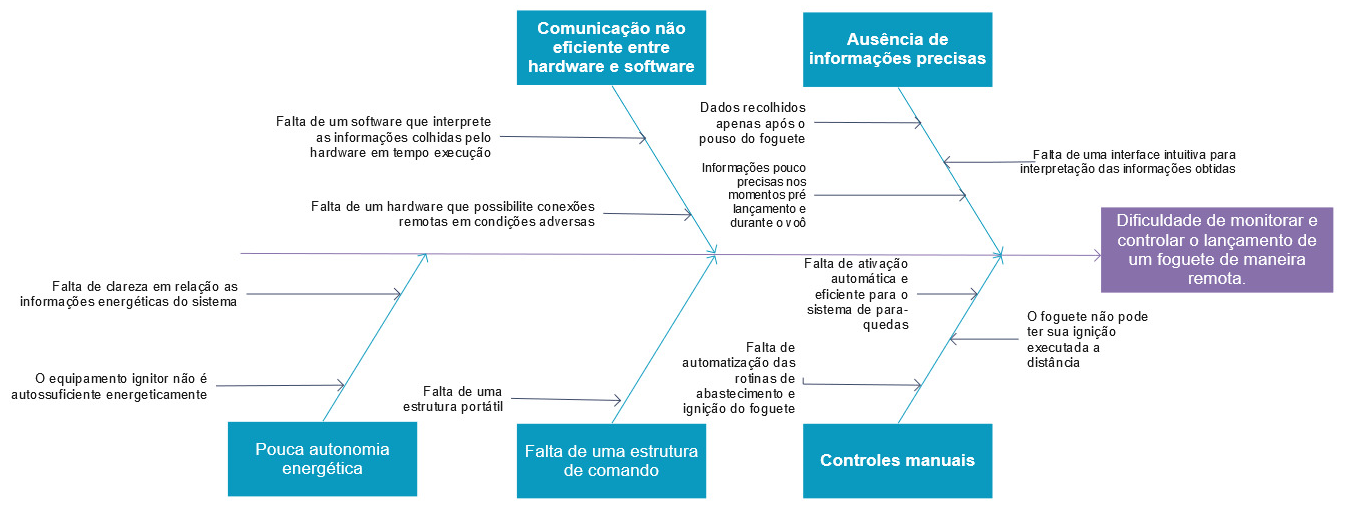
\includegraphics[width=0.9\textwidth]{figuras/Fishbone}
\caption{\textit{Fishbone}}
\label{fig:fishbone}
\end{figure}

\section{Justificativa}

\par Há dois pontos que precisam ser fundamentados a respeito do projeto: a escolha da demanda e a natureza da solução proposta para essa demanda. Quanto à escolha da demanda, optou-se por atender um problema concreto enfrentado por um agente que atua efetivamente na área de tecnologia. Ainda que o propósito principal da equipe seja de fato atender as diretrizes estabelecidas pela matéria, adotar um \textit{stakeholder} adicional traz a dupla vantagem de: a) definir requisitos do projeto de maneira clara, uma vez que o que se precisa ou não fazer é expresso pelo trabalho que o cliente já desenvolve; e b) dar destinação útil ao projeto (caso aprovado) após o fim da matéria, o que está em consonância com o propósito do curso de promover o desenvolvimento de produtos que tenham aplicação prática e/ou potencialmente comercial.

\par Quanto à natureza da solução, acreditamos que o projeto está voltado a tornar uma rotina de trabalho mais eficiente e segura. Como vimos nos requisitos de segurança das competições, uma plataforma que automatize uma série de tarefas necessárias para a preparação do lançamento de um foguete é mais do que bem-vinda, em favor da segurança dos membros de uma equipe de competição. Ademais, o cliente já reportou dificuldades passadas quanto a essas tarefas, em particular o abastecimento do tanque e o desacoplamento da mangueira, feitos com um sistema de cordas e polias em caráter contingencial. 

\par Desenvolver uma solução definitiva para essas atividades acessórias permitirá que o cliente torne mais produtivo seu trabalho voltado especificamente no desenvolvimento do seu foguete e, quem sabe, o trabalho de outras equipes interessadas e que atuem em projetos semelhantes, o que, em última análise, ajudará no desenvolvimento da atividade espacial brasileira como um todo.

%\input{editaveis/aspectosgerais}
%Aqui está sendo incluído o controle de secções
\chapter{Escopo}
\label{escopo}

\section{Metodologia de elucidação do escopo e do produto}

\par \textit{Lean Inception} é o nome dado ao método colaborativo para alinhar um grupo de pessoas sobre o MVP (produto mínimo viável) que será desenvolvido. É uma sequência de atividades para alinhar e definir objetivos, estratégias e o escopo do produto.\cite{caroli2014lean} 
\par O produto mínimo viável, em Inglês\textit{  Minimum Viable Product} (MVP), é a versão mais simples de um produto que pode ser disponibilizada para o negócio. O MVP determina quais são as funcionalidades mais essenciais para que se tenha o mínimo de produto funcional que possa agregar valor para o negócio (produto mínimo) e que possa ser efetivamente utilizado e validado pelo usuário final (produto viável). \cite{moogk2012minimum}
\par O nome\textit{ Inception }vem do RUP (\textit{Rational Unified Process}). \textit{Inception} é a primeira de quatro fases do RUP: \textit{Inception, Elaboration, Construction e Transition.} Na fase de \textit{Inception} é realizada a análise sobre os objetivos, a arquitetura e o planejamento do projeto. Isso acontece por meio de entrevistas com os \textit{stakeholders}, reuniões de alinhamento e dinâmicas de equipe. As informações obtidas nessas atividades são convertidas em requisitos descritos no formato de casos de uso. \cite{caroli2014lean} 
\par Apesar de a metodologia RUP ter sido adotada pela equipe, optou-se por não utilizar  casos de uso para delimitar as funcionalidades do produto, pois eles caíram em desuso, e os métodos ágeis adotaram o formato de histórias do usuário, que são mais focadas nos usuários do produto e entregam mais fidelidade sobre as necessidades destes. Assim, podemos definir nosso desenvolvimento do produto como \textit{user centered development}. Portanto, seguindo a nova metodologia adaptada, atividades sobre os usuários e suas jornadas são feitas (influência de \textit{design thinking} e \textit{user-centric design}); muitas histórias dos usuários são escritas, estimadas, arquitetadas e colocadas em um plano: o plano de \textit{release} do produto. 
Para elucidar e definir os requisitos, as técnicas utilizadas pela equipe foram as seguintes: 
\begin{itemize}

\item Escrita da visão de produto dinamicamente 
\item Desenvolvimento de um diagrama de causa e efeito 
\item Elaboração da estrutura analítica do projeto 
\item Método \textit{Rich Picture} 
\item Definição dos objetivos gerais e específicos
\item Definição dos requisitos 
\item É /não é, faz/não faz

\end{itemize}
\par Nos tópicos a seguir, pode-se verificar em detalhes como cada artefato foi elaborado, bem como os resultados obtidos a partir de cada artefato gerado pela equipe.
\section{Escrita da visão do produto dinamicamente}
\par Antes de iniciar a construção do produto, é importante que seja estabelecida uma visão compartilhada junto à equipe e aos demais envolvidos. Esse artefato, portanto, ajuda a manter o foco e a clareza quanto aos objetivos do produto e proporciona a horizontalidade e a distribuição de conhecimentos em relação esse produto. Uma das maneiras encontradas pela equipe para realizar essa atividade foi a elaboração de uma dinâmica de escrita da visão do produto de forma dinâmica, onde após toda a equipe reunida, realizou-se uma dinâmica de escrita coletiva de pontos importantes para a realização do produto. Após a dinâmica, foi gerado um artefato resultante que foi disponibilizado para a equipe e os \textit{stakeholders}. 

\begin{figure}[H]
\centering
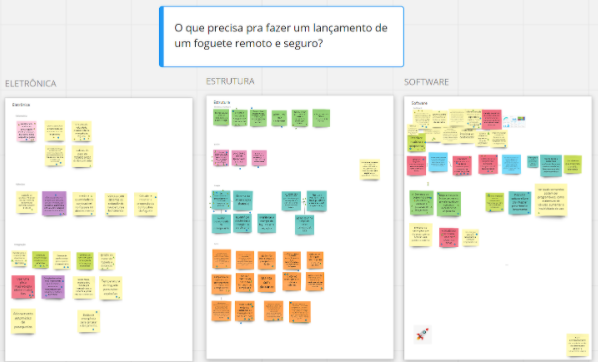
\includegraphics[scale=0.8]{figuras/miro.png}  
\caption{Ideias iniciais para solucionar o problema.}
\footnotesize Pode-se acessar em: \url{https://miro.com/app/board/o9J_kmVCAxA=/ }
\label{fig:miro }
\end{figure}

\section{Objetivos Gerais}

\par O objetivo geral do projeto é desenvolver uma tecnologia que proporciona de maneira segura o controle a longa distância do lançamento de foguetes de pequeno porte e a transmissão dos dados de voo para a central de comando (\textit{Ground Station}), ou seja, uma estação de controle de solo onde é possível controlar o abastecimento e o lançamento do foguete e receber os dados coletados durante o voo por uso da telemetria, contendo um interfaceamento intuitivo e versátil para o usuário.

\section{Objetivos Específicos}

\subsection{Eletrônica}

\par O subgrupo de eletrônica tem como objetivo  desenvolver a solução de sistema embarcado que será utilizado no projeto o que inclui: a) telemetria, que consiste no modo de transmissão de dados e sinais de controle a longas distâncias; b) sensoriamento, que consiste na captação dos estímulos físicos e a emissão de  sinais que possam ser convertidos novamente nos dados relevantes para análise do voo do foguete; c) hardware principal, que permite interfaceamento com o usuário.

\par Primeiramente serão levantados os requisitos, em conjunto com as áreas de software e energia, para melhor definição da solução e dos componentes. Em seguida, com a definição dos componentes, será feita uma bateria de testes dos sensores e periféricos com microcontroladores e microprocessadores,Umas das técnicas mais populares para documentar ideias de maneira rápida é o brainstorm. No entanto, essa técnica exige muito esforço para ser aplicada em grupo devido a dificuldade de organização das ideias e do gerenciamento de conflitos.
O brainwriting é a aplicação da técnica do brainstorm de maneira silenciosa, proposto para substituir o brainstorm em grupos. 
“Brainwriting é a geração silenciosa e escrita de ideias por um grupo de pessoas”
Existem 6 maneiras distintas de se fazer um brainwriting,
Nominal Group Technique (NGT)
Collective Notebook (CNB)
Brainwriting Pool
Pin Cards
Battelle-Bildmappen-Brainwiiting (BBB)

Para execução do brainwriting no nosso contexto, foram feitas algumas adaptações a partir do entendimento e aplicação de cada uma das técnicas.
Foi utilizada uma combinação das técnicas “Brainwriting Pool” e  “Nominal Group Technique (NGT)”, resultando na seguinte definição:
O organizador deve identificar um tema central da sessão, um problema. 
Cada participante vai usar seu espaço no MIRO para fazer um brainstorm silencioso durante 5 minutos cronometrados.
Após os primeiros 5 minutos os participantes vão usar o espaço do colega do lado pra fazer suas próprias anotações por mais 5 minutos (pode se repetir). 
Após a segunda ou terceira interação (dependendo do organizador) cada participante volta para seu espaço e lê suas ideias para o grupo, nessa etapa os integrantes podem fazer perguntas e comentários para ajudar a entender melhor a ideia em questão.
Após todos integrantes terem lido e entendido o que foi feito, todas idéias serão agrupadas de acordo com sua similaridade ou proximidade.
Cada participante receberá 1 estrela, 3 triângulos e 5 bolas. Os elementos valem: Estrela - 5 pontos, triângulo 3 pontos, bola 1 ponto.
Critério de desempate: O critério de desempate é a quantidade de elementos com pontuação maior
Os integrantes terão 5 minutos para distribuir seus pontos entre as ideias selecionadas na etapa anterior.
Ao fim da dinâmica é feita a contagem dos pontos e eleição das ideias que serão aproveitadas pelo grupo em ordem de prioridade.


Utilizando essa metodologia, conseguimos estabelecer uma visão compartilhada junto à equipe e aos demais envolvidos sobre o produto que seria desenvolvido. O artefato gerado ajuda a manter o foco e a clareza quanto aos objetivos do produto e proporciona a horizontalidade e a distribuição de conhecimentos em relação ao mesmo.
 para que assim haja a implementação do conjunto que compõe o sistema como um todo. 
\par Por fim, os ajustes finos de calibração e integração com software serão priorizados, para que seja atingida uma melhor experiência por parte do usuário.

\subsection{Energia}
\par O subgrupo de energia teve como objetivo realizar o dimensionamento elétrico do sistema como um todo, para escolher as características de um banco de baterias que suporte a alimentação dos dispositivos em um intervalo de tempo desejado. Foi preciso levar em conta que o sistema é projetado para funcionar em locais remotos e, por isso, não será possível ligá-lo à rede elétrica.
\par Também será projetado um carregador móvel para que, após o lançamento, quando necessário, seja possível conectar o sistema à rede elétrica e assim carregar a bateria.

\subsection{Software}
\par Para garantir a eficiência no uso do equipamento, a equipe deverá implementar uma interface gráfica intuitiva e adaptativa que seja capaz de receber os dados de leitura realizados pelo hardware e, após uma análise, efetuar a estruturação dos dados. Além disso, deverá garantir que o controle do abastecimento, a ignição e a abertura do paraquedas do foguete aconteçam de forma remota por meio do envio de comandos executados pelo operador do equipamento.  
\par Também será realizada a captação de informações a respeito das condições climáticas, do estado de saúde do equipamento e das informações relacionadas ao lançamento e ao voo do foguete em tempo de execução. A equipe deverá também realizar a análise quantitativa dos dados obtidos e disponibilizar graficamente os resultados por meio do sistema. 

\subsection{Estrutura}
\par O subgrupo de estrutura ficou responsável pelo desenvolvimento físico da estação de controle e de três dispositivos periféricos, responsáveis pela atuação física da abertura e do fechamento de válvulas do sistema de alimentação do foguete.
\par Quanto à estrutura da estação de controle, será desenvolvido um \textit{case} capaz de comportar um sistema de hardware complexo, com componentes eletrônicos embarcados por um software de alto nível. É esperado que o sistema seja usado em locais remotos, com presença de elementos ambientais adversos, como poeira ou mesmo umidade. Essa estrutura deve ser ainda leve e facilmente transportável, o que influencia na escolha dos materiais de que será feita. Por fim, a estrutura da estação será dimensionada para possuir uma região de armazenamento para os componentes ignitores, além de garantir a proteção dos componentes internos contra eventuais cargas externas.
\par Das estruturas periféricas, a estrutura se encarregará, junto da eletrônica, do desenvolvimento de um sistema que faça a abertura física das válvulas do sistema de alimentação de forma remota. Nesse sentido, serão desenhadas estruturas que conectam as válvulas utilizadas nesse sistema com um sistema eletromecânico que consiga receber o sinal da estação e aplicar o torque necessário para abertura ou fechamento dessas válvulas.

\section{Requisitos Gerais}
\par O \textit{Rocket Guide Station} (RGS) será um equipamento criado com a finalidade de tornar mais fácil e seguro o lançamento de foguetes de propulsão híbrida, levando em consideração os requisitos gerais a seguir:

\begin{table}[H]

\begin{tabular}{ | m{2cm} | m{12cm}|} 
 \hline
 \textbf {Requisito} & \begin{center}\textbf{Descrição} 
 \end{center}\\ 
 \hline
 RGS01 & Realizar o abastecimento e o lançamento de foguetes de propulsão híbrida de pequeno porte de forma remota e segura. \\ 
 \hline
 RGS02 & Obter informações relativas ao voo do foguete em tempo real.	 \\ 
 \hline
\end{tabular}
\caption{Requisito Gerais}
\label{Requisito Gerais}
\end{table}

\section{Requisitos Específicos}
\subsection{Estrutura}


\begin{table}[H]
\begin{tabular}{ | m{2cm} | m{12cm}| } 
 \hline
 \textbf{Requisito} & \begin{center}\textbf{Descrição}
   
 \end{center} \\ 
 \hline
 RFEST01 & Ser de uso intuitivo para o usuário.\\
 & \\
\hline
 RFEST02 & Estrutura física compacta e portátil, que dê suporte aos componentes internos da estação. \\
 \hline
 RFEST03 & Material leve e resistente, capaz de proteger os componentes internos da estação de eventuais impactos e intempéries provenientes do ambiente e de seu deslocamento. \\
  \hline
RFEST04 & Possuir um espaço na estrutura para o armazenamento do sistema de ignição. \\
\hline
RFEST05 & Ter um sistema de transmissão de torque do atuador para a válvula-esfera do sistema de abastecimento. \\
\hline
RFEST06 & Proteger o sistema eletrônico e não gerar interferência neste.  \\
\hline
RFEST07 & Estrutura interna acessível e de fácil manutenção. \\
\hline
RFEST08 & Sistema de abastecimento baseado nos componentes definidos pelo cliente. \\
\hline
\end{tabular}
\label{Requisitos de Estrutura}
\caption{Requisitos de Estrutura}
\end{table}

\subsection{Software}

\begin{table}[H]
\begin{tabular}{ | m{2cm} | m{12cm}| } 
 \hline
 \textbf{Requisito } & \begin{center} \textbf{Descrição}\end{center}\\
 \hline
 RFSW01 & O sistema deve permitir interação do usuário com a interface.\\
 \hline
 RFSW02 & O sistema deve permitir ao usuário visualizar o índice de sucesso com base de modelos estocásticos do voo em tempo de execução. \\
 \hline
 RFSW03 & O sistema deve exibir dados relevantes para a análise do operador. \\
 \hline
 RFSW04 & O sistema deve armazenar informações sobre o lançamento e voo de foguetes de forma indexada. \\
 \hline
 RFSW05 & O sistema deve ser capaz de enviar sinais a periféricos. \\
 \hline
 RFSW06 & O sistema deve ser capaz de interpretar os dados recebidos dos periféricos. \\
 \hline
\end{tabular}
\label{Requisitos de Software}
\caption{Requisitos de Software}
\end{table}


\subsection{Eletrônica}

\begin{table}[H]
\centering
\begin{tabular}{| m{2cm} | m{12cm}| } 
 \hline
 \textbf{Requisito} & \begin{center}\textbf{Descrição}\end{center} \\ 
 \hline
 RFEL01 & O sistema deve realizar o controle de toda parte sensorial\\
 &acoplada aos microcontroladores e microprocessador.\\
 \hline
 RFEL02 & O sistema deve ser capaz de monitorar o peso do foguete antes do lançamento.\\ 
 \hline
 RFEL03 & O sistema deve mandar um sinal para o aquecimento da resistência da ignição do foguete.\\ 
 \hline
 RFEL04 & O sistema deve fazer o uso de telemetria para o colhimento dos dados do foguete e seu controle.\\ 
 \hline
 RFEL05 & A RGS deve comunicar-se numa distância mínima de 1.5Km.\\ 
 \hline
 RFEL06 & O sistema deverá funcionar independentemente do acesso à internet.\\ 
 \hline
\ RFEL07 & A comunicação entre o foguete e o controle do usuário deverá ser feita sem fios.\\ 
 \hline
 RFEL08 & Os controles do acionamento das válvulas, acionamento da ignição, aferição dos combustíveis e do peso, visualização dos dados de GPS altitude deverão estar integrados na interface do usuário. \\ 
 \hline
 RFEL09 &  O sistema deverá ter um \textit{display} para mostrar os dados de telemetria/monitoramento (Hardware +  Software).\\ 
 \hline
 RFEL10 &  O sistema deverá ter periféricos para interação com o usuário (botões ou teclado) (Hardware + Software).\\ 
\hline

\end{tabular}
\label{Requisitos de Eletrônica}
\caption{Requisitos de Eletrônica}
\end{table}


\subsection{Energia}

\begin{table}[H]
\centering
\begin{tabular}{ | m{2cm} | m{12cm}|} 
 \hline
 \textbf{Requisito} & \begin{center} \textbf{Descrição }\end{center}\\ 
 \hline
 RFEN01 & Sistema elétrico portátil que engloba o armazenamento de  energia e a alimentação do sistema  com dispositivos leves e compactos.\\
 \hline
 RFEN02 &  Autonomia energética para no mínimo 2 horas de operação e no máximo 3 horas (intervalo de tempo que leva em média para o lançamento do foguete). \\ 
 \hline
 RFEN03 & Sistema elétrico capaz de alimentar os dispositivos de ignição. \\
 \hline
 RFEN04 & Carregador móvel de bateria que utilizará a rede elétrica.\\

 \hline
\end{tabular}
\label{Requisitos de Energia}
\caption{Requisitos de Energia}
\end{table}


\subsection{Requisitos de Usabilidade }

\begin{table}[H]
\centering
\begin{tabular}{ | m{2cm} | m{12cm}| } 
 \hline
 \textbf{Requisito} & \begin{center} \textbf{Descrição} \end{center}\\ 
 \hline
 RUSW01  & A interação do usuário com a interface do produto deverá ser intuitiva.\\
 \hline
 RUSW02 & A interface deverá possuir prevenção e notificação de erros, caso o \\& preenchimento de dados for incorreto. \\ 
 \hline
 RUSW03 & O produto deve ser suficiente energeticamente durante o voo.\\ 
 \hline
 RUSW04 & As rotinas manuais de lançamento deverão ser, em sua maioria,  automatizadas.\\ 
 \hline
 RUSW05 & A estrutura deverá comportar os componentes eletrônicos da própria estação \\& e possuir um espaço sobressalente. \\ 
 \hline
 RUSW06 & Os módulos do sistema deverão comunicar-se por meio de rádio frequência.\\ 
 \hline
 
\end{tabular}
\label{Requisitos de Usabilidade}
\caption{Requisitos de Usabilidade}
\end{table}

\section{Lista É/Não É}
\par A dinâmica de É/Não É é uma atividade que ajuda a identificar o escopo, as limitações do produto e os aspectos que devem ser realmente considerados na hora do desenvolvimento. Trata-se de uma matriz onde, por meio de uma discussão de equipe, definem-se as características, e também aquilo que não serão características, do produto. O quadrante “É”, deve ser preenchido com tudo aquilo que o produto que será desenvolvido é, e o quadrante “Não é” com tudo aquilo que o produto não deve ser.

\begin{center}
\begin{table}[H]

\begin{tabular}{ | m{7cm} | m{7cm}| } 
 \hline
\begin{center}\textbf{É }\end{center} & \begin{center} \textbf{NÃO É}\end{center}   \\ 
 \hline
É capaz de receber e mandar dados de controle com o foguete e sua base. & Não é à prova d’água. \\ 
 \hline
 É capaz de mandar sinais de controle para válvulas do abastecimento e para ignição do foguete. & Não é capaz de parar o lançamento após a ignição. \\ 
 \hline
É capaz de colher dados de sensores no foguete e enviar para a visualização do usuário. & Não é capaz de comunicar-se a distâncias maiores que 2 km. \\ 
 \hline
É capaz de mostrar os dados por meio de uma tela. & Não é capaz de comunicar-se com a internet.\\ 
 \hline
 É capaz de receber comandos do usuário por meio de um teclado. & Não é um computador pessoal (uso geral). \\
 \hline
 É capaz de comunicar-se de forma sem fio entre os microcontroladores. & Não é capaz de desabastecer o foguete \\
 \hline
 É capaz de armazenar os dados dos sensores do foguete em uma memória externa. & Não é um sistema de lançamento autônomo. \\
 \hline
 É capaz de coletar GPS, velocidade e apogeu do foguete. & Não é capaz de coletar a pressão interna e temperatura dentro do foguete e dados sobre a qualidade do combustível. \\
 \hline
 É um sistema autônomo e móvel com uso de bateria. & Não é conectado de forma fixa à rede elétrica. \\
 \hline
 É carregado periodicamente conforme a necessidade. & Não é totalmente independente da rede elétrica. \\
 \hline
É base de comando. & Não é uma base de lançamento. \\
\hline
É estrutura comportadora de um hardware embarcado. & Não é um foguete experimental. \\
\hline
É um sistema independente do tanque de combustível. & Não é um tanque de combustível. \\
\hline
Tem ignição eletromecânica. & Não é uma mala comum de viagem. \\
\hline
\end{tabular}
\label{Lista de É/Não É}
\caption{Lista de É/Não É}
\end{table}
\end{center}


\chapter{TERMO DE ABERTURA DO PROJETO}
\section{Introdução}
O lançamento de um foguete experimental de propulsão híbrida exige procedimentos de preparo e abastecimento que devem ser executados à distância da base de lançamento. Do mesmo modo, é recomendável fazer a coleta dos dados do foguete (em particular sua localização e altitude) durante o voo. O uso de uma estação de controle e monitoramento remoto faz-se necessário.

\section{Justificativa do Projeto}
A \textit{Rocket Guide Station} (RGS) é uma estação remota capaz de realizar a abertura e fechamento das válvulas que compõem o sistema de alimentação utilizado pela \textit{Capital Rocket Team}, cliente da equipe, bem como de executar a ignição do foguete no momento de seu lançamento. Além disso, é capaz de receber os dados de telemetria do foguete durante o voo. O uso dessa estação não somente otimizará o trabalho do cliente na execução dessas tarefas acessórias a uma missão de lançamento, como também poupará eles de terem de desenvolver uma estação por conta própria, possibilitando que eles se dediquem à sua função principal, que é o desenvolvimento do foguete em si.

\section{Stakeholders}
\label{stakeholders}


\subsection{Equipe} A equipe é composta por alunos da disciplina Projeto Integrador da Faculdade do Gama da Universidade de Brasília (tabela \ref{tab:equipe}). E tem o compromisso de entregar o produto de acordo com o escopo acordado entre o professor da disciplina e os integrantes do time;

\begin{table}[H]
\centering
\begin{tabular}{|l|l|l|}
\hline
Nome & Curso & e-mail \\ \hline
    André Hernandez Bargas &    Software   &    andrebargas@gmail.com    \\ \hline
    Artur Cardoso de Almeida &    Automotiva   &    artur.kd2@gmail.com    \\ \hline
    Augusto Moreno Vilarins  &   Software    &    augusto.vilarins@gmail.com    \\ \hline
    Diogo Filipe Sens &     Aeroespacial   &    diogosens@gmail.com    \\ \hline
    Douglas Alves Brandão  &    Aeroespacial   &   douglasbbb@gmail.com     \\ \hline
    Francisco Matheus Fernandes Gomes &   Eletrônica    &    f.matheusbsb@gmail.com    \\ \hline
    Gabriela Alves da Gama &    Software   &    gabrielaalvesdagama@gmail.com    \\ \hline
    Gustavo Cavalcante Linhares &     Eletrônica   &  gugacavalcante.10@hotmail.com      \\ \hline
    Isaque Alves de Lima &   Software    &    isaquealvesdl@gmail.com    \\ \hline
    João Henrique Egewarth &    Software    &    egewarth@gmail.com    \\ \hline
    Luísa Prospero de Carvalho Silva &   Aeroespacial   &    luisaprosperocs@gmail.com    \\ \hline
    Milena Martins Magalhães &   Energia    &    milenammagalhaes@gmail.com    \\ \hline
    Misael de Souza Andrade &     Eletrônica   &    misas.andrade@gmail.com    \\ \hline
    Thainá Rodrigues Fernandes &   Energia    &    thaina_rodrigues.f@hotmail.com    \\ \hline
\end{tabular}
\caption{Equipe do Projeto}
\label{tab:equipe}
\end{table}
    
\subsection{Professores} São apoiadores e avaliadores do projeto, que auxiliam na decisão da metodologia, escopo, produção e aspectos técnicos relacionados à solução do problema;

\begin{itemize}
    \item Alex Reis - Engenharia de Energia
    \item José Felício da Silva - Engenharia Eletrônica
    \item Paolo Gessini - Engenharia Aeroespacial
    \item Rhander Viana - Engenharia Automotiva
    \item Ricardo Matos Chaim - Engenharia de Software
\end{itemize}
    
\subsection{Capital Rocket Team - CRT} Cliente, tem o encargo de fornecer os requisitos necessários para a construção do projeto, além de fornecer  insumos para a construção do produto.

\begin{itemize}
    \item e-mail: capitalrocketteam@gmail.com
    \item Número: (61) 99853-9777
    \item Redes sociais: @capitalrocketteam
\end{itemize}

\section{Matriz SWOT}

A matriz SWOT, também conhecida como matriz FOFA, é uma ferramenta gerencial que examina o ambiente interno e externo de uma organização, buscando identificar as as suas forças, fraquezas, oportunidades e ameaças, para encontrar oportunidades de melhoria e otimização do desempenho\cite{santella_MatrizSWOT_blog2020}.

A figura \ref{fig:matrizSWOT} apresenta a matriz SWOT, com a análise desses quatro elementos de acordo com o contexto do projeto proposto.

\begin{figure}[H]
  \centering
  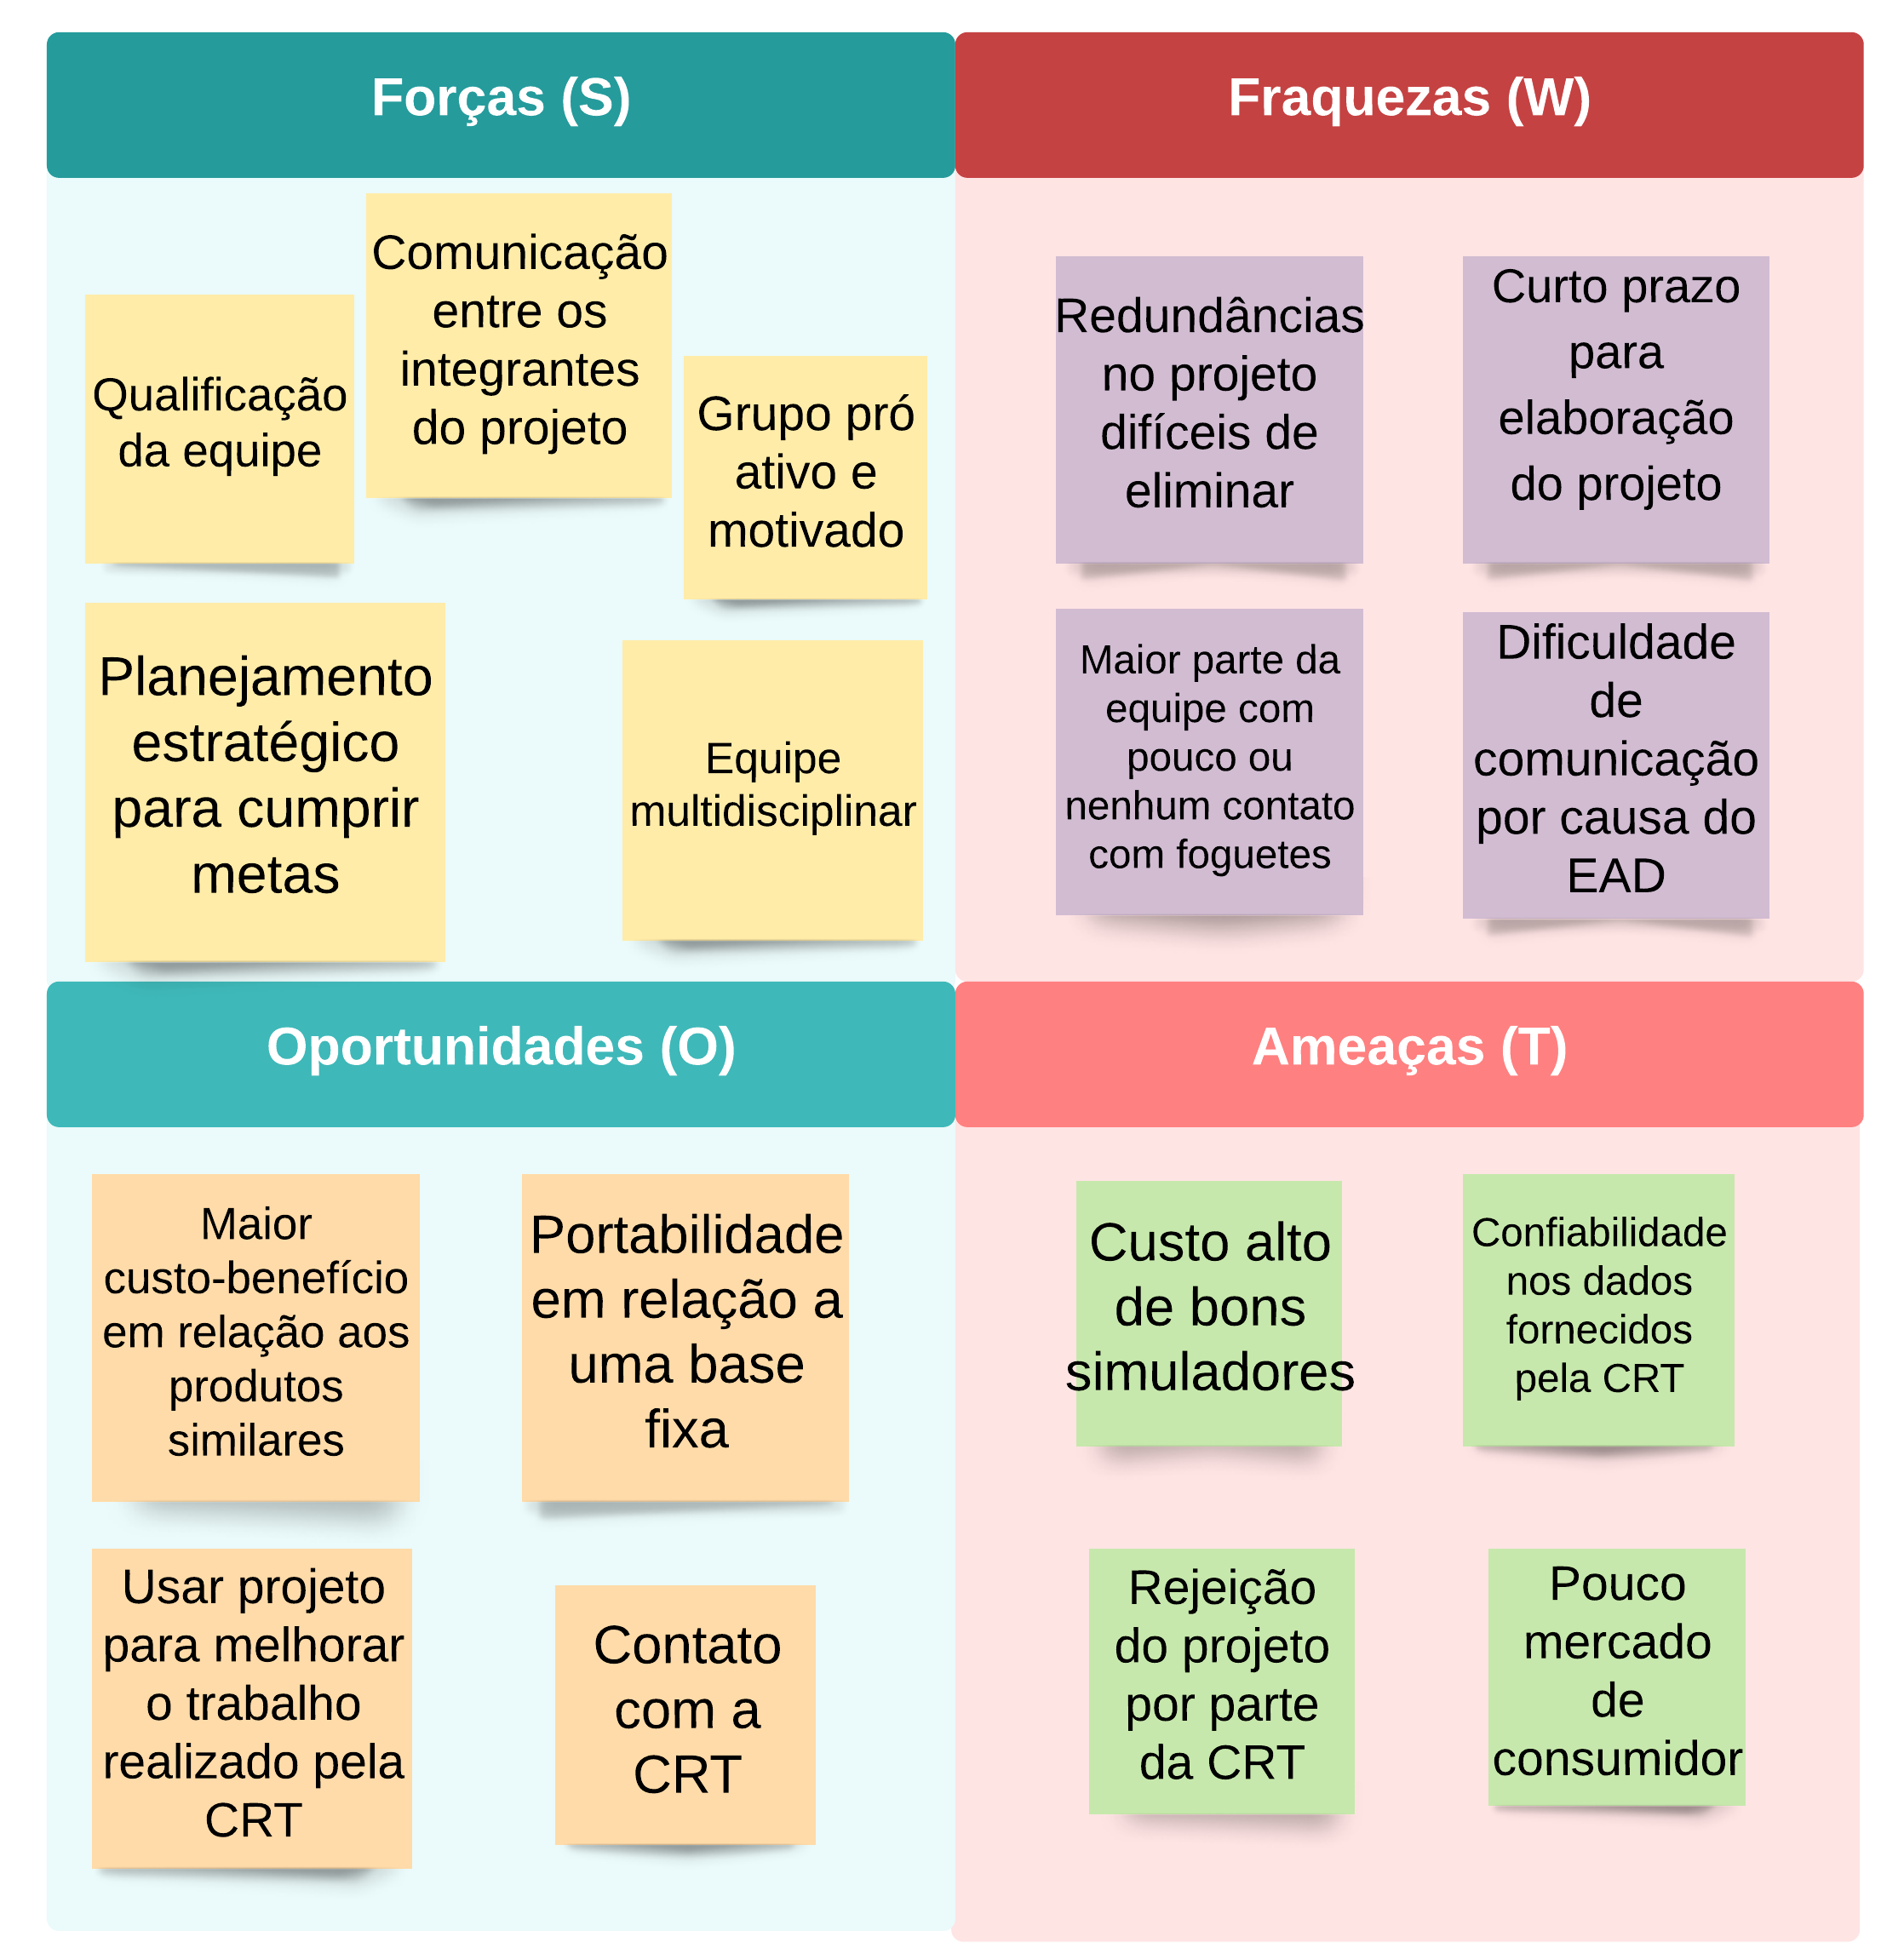
\includegraphics[scale=0.15]{figuras/SWOT_BaseLancamento.png}
  \caption{Matriz \textit{SWOT}. Matriz foi construída usando a ferramenta Lucidchart.} 
  \label{fig:matrizSWOT}
\end{figure}
\section{5W1H}

Antes de iniciar um projeto é muito importante ter com clareza: o que vai ser feito, como deve ser feito, porque deve ser feito, quem será responsável pelo trabalho, onde será feito e em qual período de tempo. A resposta para essas perguntas aprimoram o planejamento e auxiliam na criação de um plano de ação \cite{5w1hUFMG}.

A figura \ref{fig:5w1h} apresenta em forma de diagrama cada uma das 6 perguntas fundamentais e suas respectivas respostas baseadas no contexto desse projeto.

\begin{figure}[H]
  \centering
  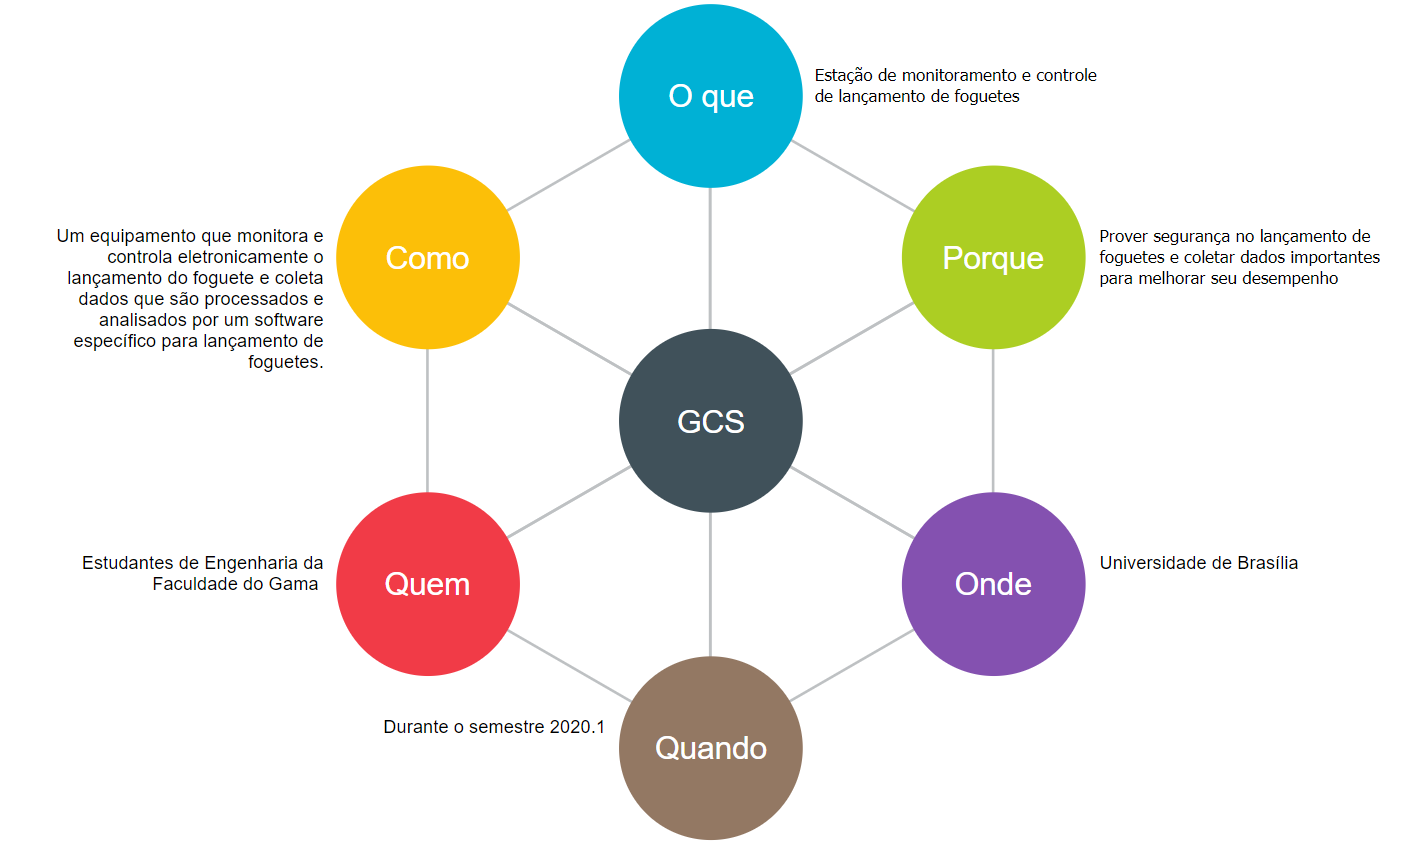
\includegraphics[width=\textwidth,height=\textheight,keepaspectratio]{figuras/5w1h.png}
  \caption{5W1H. O diagrama foi construído usando a ferramenta Visual Paradigm Online Diagrams.} 
  \label{fig:5w1h}
\end{figure}

\section{Bussines Model CANVAS}

Com o uso da ferramenta MIRO, foi desenvolvido um  \textit{business model} Canvas para o projeto, que pode ser visto no apêndice \ref{canvas}:  figura \ref{fig:Canvas} . Comumente chamado apenas de Canvas, essa ferramenta tem como objetivo esboçar a ideia de um modelo de negócio de maneira simples, eficaz e visual. Logo, um documento como este agrega valor ao projeto, devido ao fato deste estar ligado à uma equipe de competição.

Exemplificando, de acordo com o desempenho da equipe nas competições, a atenção dos outros competidores voltar-se-á ao projeto. Dada essa relação, poderão surgir  oportunidades de realizar negócios por meio do produto desenvolvido, assim justificando o desenvolvimento e o valor desse documento.  


\section{Estrutura Analítica do Projeto}

Com a necessidade de definir os objetivos e as entregas do projeto, foi criada a Estrutura Analítica do Projeto (EAP) na ferramenta \textit{Mindmeister}. O objetivo desse documento é fazer o planejamento de alto nível das atividades e dos objetivos do projeto, divididos em pacotes de entregas conhecidos como Pontos de Controle (PC). Esse documento será utilizado para fazer o planejamento das  \textit{sprints} de cada PC, para auxiliar na comunicação com os  \textit{Stakerholders}, pois ele detalha e define quais atividades e evoluções estão previstas para cada PC.

A EAP foi definida e acordada entre o Gerente Geral, o Diretor de Qualidade e os Diretores Técnicos. Levando em consideração as necessidades dos \textit{Stakerholders} e do contexto da disciplina. Como apresentado na Imagem \ref{fig:EAP}, o projeto está organizado em 3 pontos de controle, também conhecidos como \textit{Releases}, que consistem em pacotes de entrega que agreguem valor ao projeto e atendam às necessidades definidas no Plano de Ensino. Dentro de cada uma das entregas, estão as grandes frentes de desenvolvimento do Projeto, as quais são: Documentação/Viabilidade Técnica, Software, Eletrônica, Estrutura e Energia.

Em cada uma dessas frentes, estão definidas as atividades macro, ou os objetivos a serem alcançados e entregues nessa  \textit{Release}. Vale lembrar que a metodologia principal do projeto é Ágil, logo as atividades e objetivos podem ser alterados de acordo com a necessidade e a evolução do projeto.
\section{ \textit{Roadmap}}
Para uma melhor visualização e análise do  \textit{Roadmap}, ele pode ser visto no Apendice \ref{Roadmap}, mas também está disponível no link a seguir: \href{https://docs.google.com/spreadsheets/d/13mSpMqhIIh5OHl95djhCfA4ejr36CvJLpA65PvluUAU/edit?usp=sharing}{ \textit{Roadmap}}.

\subsection{Marcos Identificados}
\label{Milestones Identificados}
Os \textit{milestones} identificados encontram-se na tabela \ref{tab:tabelamilestones}. 




\begin{table}[H]
\begin{tabular}{|p{8cm}|p{6cm}|}
\hline
%%%%%%%%%%%%%%%%%%%%%%%%%%%%%%%%%%%%%%%%%%%%%%%%%
\textbf{Atividades}  & \textbf{Data de Entrega}         
\\ \hline
%%%%%%%%%%%%%%%%%%%%%%%%%%%%%%%%%%%%%%%%%%%%%%%%%

Entrega de Relatório Ponto de Controle 1    & 5 dias antes da apresentação
\\ \hline
%%%%%%%%%%%%%%%%%%%%%%%%%%%%%%%%%%%%%%%%%%%%%%%%%

Apresentação Ponto de Controle 1 &  18/09/2020, 25/09/2020 ou 02/10/2020

\\ \hline
%%%%%%%%%%%%%%%%%%%%%%%%%%%%%%%%%%%%%%%%%%%%%%%%%

Entrega de Relatório Ponto de Controle 2  & 5 dias antes da apresentação 
\\ \hline
%%%%%%%%%%%%%%%%%%%%%%%%%%%%%%%%%%%%%%%%%%%%%%%%%

Apresentação Ponto de Controle 2 & 16/10/2020, 23/10/2020 ou 30/10/2020
\\ \hline
%%%%%%%%%%%%%%%%%%%%%%%%%%%%%%%%%%%%%%%%%%%%%%%%%

Entrega de Relatório Ponto de Controle 3 & 5 dias antes da apresentação
\\ \hline
%%%%%%%%%%%%%%%%%%%%%%%%%%%%%%%%%%%%%%%%%%%%%%%%%
Apresentação Ponto de Controle 3 & 13/11/2020, 20/11/2020 ou 27/11/2020
\\ \hline
%%%%%%%%%%%%%%%%%%%%%%%%%%%%%%%%%%%%%%%%%%%%%%%%%
Entrega do repositório do projeto & 04/12/2020
\\ \hline
%%%%%%%%%%%%%%%%%%%%%%%%%%%%%%%%%%%%%%%%%%%%%%%%%
Apresentação de projetos na FIT/FGA On Line
(Feira de Inovação e Tecnologia da FGA) & 04/12/2020

\\ \hline
%%%%%%%%%%%%%%%%%%%%%%%%%%%%%%%%%%%%%%%%%%%%%%%%%
\end{tabular}
\caption{ \textit{Milestones} identificados.}
\label{tab:tabelamilestones}
\end{table}
\section{Viabilidade Técnica}
\label{recursosHumanos}
\subsection{Metodologia}

A fase inicial do projeto, também conhecida como Ponto de Controle 1 (PC1), visa garantir a definição da Metodologia, da gestão de riscos, e as definições que farão parte do desenvolvimento. Nesse projeto, 
o objetivo principal na definição da metodologia e da cultura é garantir o desenvolvimento e a organização da condução do projeto e das atividades de acordo com praticas da comunidade Ágil e do  \textit{DevOps} já adotadas pela comunidade \cite{licorish2016adoption}. 

As práticas do  \textit{DevOps} farão parte dos objetivos principais do PC1, pois irão auxiliar na gestão do projeto, baseando-se em quatro categorias: \textit{People, Process, Delivery e Runtime} \cite{leite2019survey}. Desde o primeiro momento, foram aplicados e apresentados conceitos e práticas do  \textit{DevOps},  \textit{Lean} e Ágil. Essas práticas irão auxiliar na adoção de uma nova cultura ágil e colaborativa entre os membros do projeto para garantir a qualidade nos produtos desenvolvidos. 

Além dos conceitos técnicos e não técnicos do  \textit{DevOps}, foi adotado como base o \textit{framework Scrum}, em que empregamos processos e técnicas aos papéis, eventos, artefatos e regras, adaptando as necessidades da equipe. O objetivo do \textit{Scrum} no projeto é permitir o controle do trabalho a ser realizado por meio de uma gestão dinâmica, assim identificar obstáculos durante o processo de desenvolvimento, e reagir a eles se torna mais fácil \cite{gren2015prospects} \cite{gren2020agile} \cite{licorish2016adoption}. A abordagem interativa e incremental empregada otimiza a previsão e monitoramento de riscos.

Também adotamos o uso do  \textit{Kanban} para controle do fluxo de produção da equipe. Para a otimização do trabalho desta, foi utilizada a ferramenta  \textit{Trello}, já integrada no  \textit{MsTeams}. 

Para rastrear as tarefas e levantar dados, utilizamos o  \textit{Dashio} para coleta de Métricas e Indicadores que auxiliem as equipes. As Imagens \ref{fig:cumulativesoftware}, \ref{fig:cumulativeeletronica} e \ref{fig:cumulativeestrutura} apresentam o Gráfico \textit{Cumulative Flow} desse PC1 (Sprint 0 até 3). Pelo gráfico, podemos observar as entregas feitas a cada \textit{Sprint} (avanço no gráfico a cada 7 dias). O objetivo do time é reduzir o tempo entre as entregas para que não seja em formato de "pacotes" ao fim de cada revisão, garantindo assim uma entrega contínua. É possível observar que todos os times conseguiram fazer entregas durante a  \textit{sprint} e que na Imagem \ref{fig:cumulativesoftware} e \ref{fig:cumulativeeletronica} existem algumas distorções nos gráficos, pois os times identificaram duplicidade de atividades e arquivaram os \textit{Cards}.

\begin{figure}[H]
    \centering
  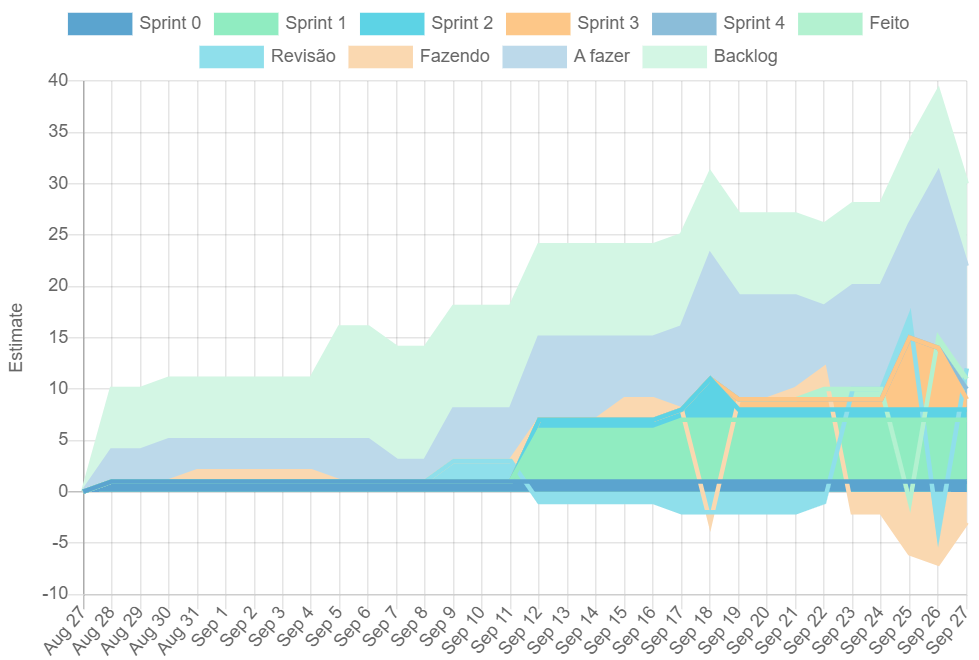
\includegraphics[scale=0.3]{figuras/cumulative_software.png}
  \caption{\textit{Cumulative Flow} da equipe de Software coletados de 27 de agosto até 26 de setembro de 2020.}
  \label{fig:cumulativesoftware}
\end{figure}
\begin{figure}[ht]
\centering
  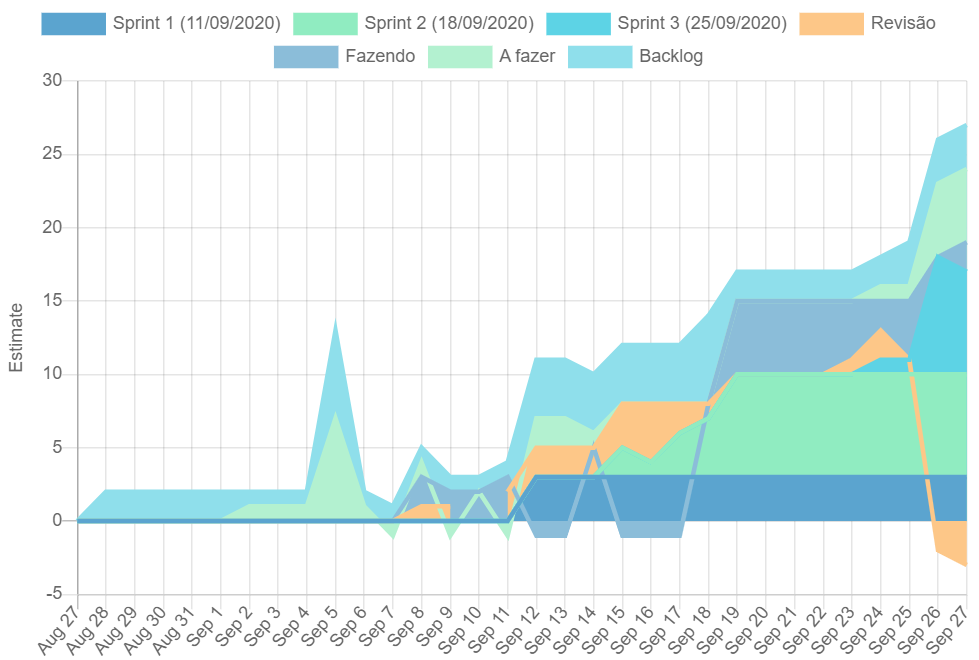
\includegraphics[scale=0.3]{figuras/cumulative_eletronica.png}
  \caption{\textit{Cumulative Flow} da equipe de Eletrônica coletados de 27 de agosto até 26 de setembro de 2020.}
  \label{fig:cumulativeeletronica}
\end{figure}
\begin{figure}[H]
\centering
  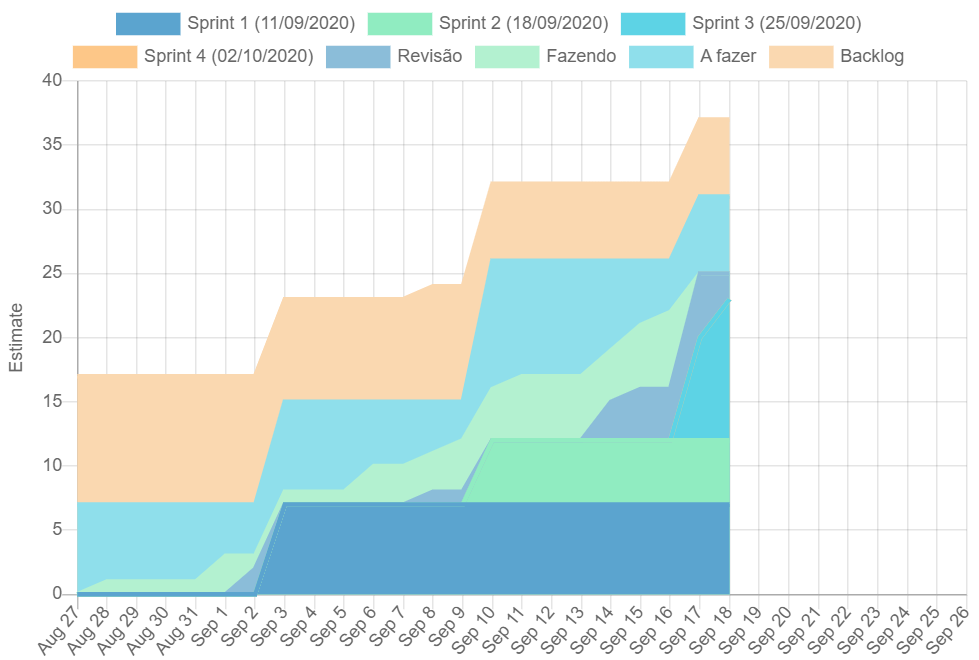
\includegraphics[scale=0.3]{figuras/cumulative_estrutura.png}
  \caption{\textit{Cumulative Flow} da equipe de Estrutura e Energia coletados de 27 de agosto até 26 de setembro de 2020.}
  \label{fig:cumulativeestrutura}
\end{figure}

Já o XP foi uma das metodologias adotadas pelo conjunto de práticas que são ditas como boas na Engenharia de Software como pareamento, refatorar o tempo todo, testar o tempo todo, entre outros.

\subsection{Papeis}
Durante o projeto, a equipe possuirá um Gerente Geral, um Diretor de Qualidade e será subdividida em 3 subgrupos, cada um contando com um Diretor Técnico (destacado em negrito):
\begin{itemize}
    \item Gerente Geral: Isaque Alves de Lima
    \item Diretor de Qualidade: Diogo Filipe Sens
    \item Estrutura e Energia
        \subitem - \textbf{Luisa Prospero de Carvalho Silva}
        \subitem - Artur Cardoso de Almeida
        \subitem - Douglas Alves Brandão 
        \subitem - Milena Martins Magalhães
        \subitem - Thainá Rodrigues Fernandes
    \item Eletrônica
        \subitem - \textbf{Gustavo Cavalcante Linhares}
        \subitem - Francisco Matheus Fernandes Gomes 
        \subitem - Misael de Souza Andrade
    \item Software
        \subitem - \textbf{João Henrique Egewarth}  
        \subitem - Andre Hernandez Bargas
        \subitem - Augusto Moreno Vilarins
        \subitem - Gabriela Alves da Gama
\end{itemize}

\subsection{Ritos Adotados}
\label{ritos}
\begin{itemize}
    \item \textit{Sprint}
        \subitem Início: sexta-feira
        \subitem Fim: sexta-feira
        \subitem Duração: 7 dias
\end{itemize}

\subsubsection{Planejamento da \textit{Sprint}}

\textbf{Duração máxima: 45 min}

A reunião de planejamento da  \textit{Sprint} é realizada semanalmente às sextas-feiras com a participação de todos os participantes separados nas suas frentes. A reunião de planejamento segue os seguintes passos:


1 - O time discute quais são as prioridades e necessidades do time;

2 - O time deve ter um objetivo bem definido para a  \textit{sprint};

3 - O time cria e seleciona as atividades que devem ser produzidas durante a  \textit{sprint};

\textbf{OBS:} Como as  \textit{sprints} são semanais, as atividades devem ser pensadas para concluir em 7 dias.

4 - Caso haja, o time deve definir e apresentar o pareamento da semana;

\textbf{OBS:} Esse pareamento deverá estar no definido na  \textit{issue}.

5 - Criar os  \textit{cards} no  \textit{Trello};

Deve conter nas  \textit{issues}:

- Titulo;

- Breve descrição;

- Responsável (no mínimo um);


\begin{itemize}
    \item\textbf{Entradas}
        \subitem \textit{Backlog} do produto;
        \subitem Último Incremento do produto;
        \subitem Desempenho na última \textit{Sprint}.
    
    \item\textbf{Saída}
        \subitem \textit{Backlog} da \textit{Sprint}.
\end{itemize}   


\subsubsection{Revisão da \textit{Sprint}}
\textbf{Duração máxima: 45 min}

\textbf{Missão:} Inspecionar o incremento e adaptar o \textit{Backlog}.

A reunião de Revisão do time é realizada semanalmente às sextas-feiras com a participação de todos os membros do time. A reunião segue os seguintes passos:

1 - O time discute e valida as atividades e artefatos produzidos durante a  \textit{sprint} que se finaliza;

2 - O time discute o \textit{Backlog} do Produto atual e se o time conseguirá atingir a meta das entregas;

3 - O grupo colabora com as soluções;

4 - É feita uma análise do mercado para definir o que é mais importante para fazer a seguir.


\subsubsection{Retrospectiva da \textit{Sprint}}
\textbf{Duração máxima: 30 min}


1 - Revisar, dentro do modelo de trabalho e das práticas do processo do  \textit{Scrum}, o processo de desenvolvimento, de forma a torná-lo mais eficaz e gratificante para a próxima \textit{Sprint};

2 - Inspecionar como correu a última \textit{Sprint} em se tratando de pessoas, das relações entre elas, dos processos e das ferramentas;

3 - Priorizar os principais itens que correram bem e aqueles que, se feitos de modo diferente, poderiam ter deixado as coisas ainda melhores.


\subsection{Ferramentas}
\begin{itemize}
    \item Teams
        \subitem Principal ferramenta de comunicação que permite o compartilhamento de vídeos, documentos e a integração com as outras ferramentas utilizadas no projeto, além de centralizar a comunicação ela é a ferramenta principal para as conferências.
    \item Drive
        \subsubitem Ferramenta em nuvem para armazenamento compartilhado. Será utilizada para compartilhar a documentação e informações entre os membros.
    \item Overleaf
        \subsubitem É uma ferramenta colaborativa de escrita online em LaTeX, cujo objetivo é facilitar todo o processo de escrita, edição e publicação de documentos.
    \item GitHub
        \subsubitem O GitHub é uma plataforma de hospedagem de código-fonte com controle de versão usando o Git.
\end{itemize} 
\section{Gestão dos Riscos}
\label{levantamentoRiscos}

A Gestão de Risco é um processo de identificação, análise, avaliação, tratamento e monitoramento de um evento que pode atrasar uma entrega de um produto ou serviço. A ISO 31000 define como atividades coordenadas para dirigir e controlar uma organização no que se refere a riscos \cite{purdy2010iso}.
Neste projeto, a gestão de risco é feita utilizando práticas da metodologia ágil, onde os riscos Técnicos, Externos, Organizacionais e relacionados ao Gerenciamento são levantados e acompanhados a cada  \textit{Sprint}, a fim de reduzir a probabilidade do risco acontecer \cite{cohn_RiskBurndown_blog2010}.

Para isso, criamos um \textit{burndown} de Riscos que auxilia no acompanhamento dos riscos por \textit{Sprints}, verificando a probabilidade e o impacto do risco, a fim de reagir a tempo. Esse modelo de gestão de riscos baseia-se em uma métrica subjetiva, pois o próprio time define o impacto e a probabilidade do risco acontecer. 

O processo de identificação, análise, avaliação, tratamento e monitoramento de um evento (interno ou externo) que pode ser um risco para o projeto é feito em todas as {\em sprints}, sendo que cada {\em sprint} cobre o período de uma semana. Primeiramente, é feito um levantamento de todos os $N$ eventos potenciais de risco ao projeto. Cada item desse levantamento é avaliado periodicamente, levando-se em conta dois fatores: a chance de o risco ocorrer $P$ e o impacto disso $I$. No nosso caso, ambos fatores ($P$ e $I$) são anotados usando valores que vão de 0 a 5, indicando as seguintes avaliações qualitativas de probabilidade de cada evento ocorrer: nenhum; raro; improvável; pouco provável; 
muito provável; quase certo. Os cálculos e o acompanhamento dos riscos estão disponíveis na planilha de Riscos por meio do link a seguir: \href{https://docs.google.com/spreadsheets/d/1TQ4I9uqX-XxH3AdRi01n4jIX4YpIWYOHws1GxpdqUF0/edit?usp=sharing}{Planilha de Acompanhamento dos Riscos}.

\begin{figure}[ht]
  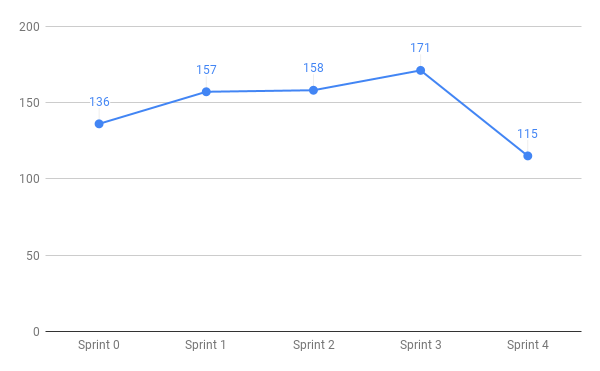
\includegraphics[scale=0.75]{figuras/burndownrisco.png}
  \caption{\textit{Risk Burndown} geral: multiplição da  probabilidade do evento do risco pelo impacto do evento no desenvolvimento do projeto, durante a Release 1.} 
  \label{fig:riscogeral}
\end{figure}

O fator {\em Risk Burndown} (eixo Y no gráfico da figura \ref{fig:riscogeral}) é calculado multiplicando-se esses dois fatores e somando os resultados para todos os $N$ eventos avaliados.
Até o momento, foram identificados $N=17$ fatores de risco, ou seja, o maior valor possível para o fator {\em risk burndown} deste projeto atualmente seria de $N \times P \times I = 17 \times 5 \times 5 = 425$, num cenário de caos absoluto.
Porém, não é de se esperar que todos os fatores tenham impacto máximo e máxima probabilidade de acontecer ao mesmo tempo, por isso o gráfico da figura \ref{fig:riscogeral} mostra o eixo Y indo somente até 200.

Durante a análise da probabilidade, são definidas ações para mitigar o risco. Desde o início do projeto, os principais riscos foram ligados à cultura e organização das atividades, definição do escopo para atender às necessidades do cliente e à pandemia. É possível notar o crescimento de risco do projeto na {\em Sprint} 3, devido a identificação de novos riscos, mas é possível notar na Imagem \ref{fig:riscogeral} que os riscos estão diminuindo constantemente.
\section{Estimativa de Custos}

Apesar de não existir a necessidade de construção do projeto este semestre, devido a situação sanitária no qual o mundo se encontra, foi construído uma tabela com os custos totais dos materiais componentes que seriam utilizados. A tabela \ref{tab:estimativa materiais} mostra um valor estimado do metro quadrado dos materiais pesquisados. 

\begin{table}[H]
\begin{tabular}{| m{4cm}|m{2cm}|m{2cm}|m{2cm}|m{2cm}|m{2cm}|}
\hline
\multicolumn{6}{|c|}{\textbf{Estrutura e Energia}}\\
\hline
Material & Preço  & Quantidade & Frete & Loja & Total  \\ 
\hline
Bateria Lítio Ferro Fosfato (UPLFP12-30) & 1.426,00  & 1 & 00,00 & Unipower & 1.426,00  \\ 
\hline
Módulo Regulador de Tensão (LM2596)   & 10,90  & 3  & 21,11 & Curto Circuito      & 53,81  \\ 
\hline
MDF   &  R\$36,81 & 1$m^2$x3mm  &   &    &  R\$36,81 \\ 
\hline
MDF   & R\$62,50  & 1$m^2$x6mm  &   &    & R\$62,50  \\ 
\hline
PRFV   & R\$52,90  & 1$m^2$  &   &    &  R\$52,90 \\ 
\hline
PRFC   &  R\$421,43 & 1$m^2$ &   &    &  R\$421,43 \\ 
\hline
PLA   & R\$140,00  & 1kg  &   &    &  R\$140,00  \\ 
\hline
ABS   &  R\$ 16,80 & 1kg  &   &    & R\$ 16,80  \\ 
\hline
 Atuador pneumático  &  entre R\$250 a R\$2000 & 2  &   &    &   \\ 
\hline
 Atuadores elétricos  & entre U\$60 a U\$240  &  2 &   &    &   \\ 
\hline

\end{tabular}
\caption{Estimativa de custos de Materiais}
\label{tab:estimativa materiais}
\end{table}

\begin{table}[H]
\begin{tabular}{| m{6cm}|m{1cm}|m{2cm}|m{1cm}|m{3cm}|m{1cm}|}
\hline
\multicolumn{6}{|c|}{\textbf{Eletrônica}}                                                 \\ \hline
Componente                & Preço  & Quantidade & Frete & Loja          & Total  \\ \hline
Jetson Nano Developer Kit  & 899,91 & 1          & 50,45 & Submarino    & 950,36 \\ \hline
TELA LCD - 9 polegadas    & 269,75 & 1          & 0,00  & arduoeletro   & 269,75 \\ \hline
Mini Teclado com touchpad & 189,14 & 1          & 0,00  & Mercado Livre & 189,14 \\ \hline
Placa LoRa Esp32          & 129,90 & 3          & 27,90 & Mercado Livre & 417,60 \\ \hline
Sensor BMP280             & 13,50  & 1          & 21,11 & Curtocircuito & 34,61  \\ \hline
Célula de carga 50kg      & 16,90  & 1          & 16,50 & Eletrogate    & 33,40  \\ \hline
Módulo Hx711              & 10,40  & 1          & 19,90 & Mercado Livre & 30,30  \\ \hline
Módulo GPS GY-NEO6MV2     & 79,90  & 1          & 19,70 & Robocore      & 99,60  \\ \hline
\end{tabular}
\caption{Estimativa de custos componentes eletrônicos}
\end{table}



Com isso o custo total dos materiais do projeto inicialmente é\textbf{ R\$ 3.504,57} reais.



\part{Concepção e Detalhamento da Solução}

\chapter{Solução Geral}

\begin{figure}[H]
    \centering
    
\includegraphics[width=0.5\textwidth]{figuras/4.png}
\end{figure}

\par A solução proposta é o projeto de uma estação de controle e monitoramento do lançamento de um foguete experimental movido a propulsão híbrida. Por meio de sensores e atuadores, a estação realizará o abastecimento e a ignição remota do foguete e, durante o voo, a coleta da telemetria deste.

\par A solução conta com duas estruturas principais em formato de maleta. A primeira é aqui tratada como maleta de controle e monitoramento, onde o sistema principal de hardware estará instalado e embarcado com o código fonte de interface do usuário. Aqui também estará a bateria de alimentação para esse sistema, além da tela e do teclado para visualizações e envios de comandos por parte do usuário. 

\par A segunda maleta é referida como maleta de suporte/apoio ao abastecimento, nela estará todos os componentes necessários para a montagem e manutenção do sistema de abastecimento a distancia, bem como uma segunda bateria para os motores e para a ignição do sistema. Ela também contará para o transporte do adaptador de válvula.

\par Por fim a solução conta com um sistema de carregamento para ambas as baterias selecionadas, um sistema de aquisição de dados de sensores que vão dentro do foguete e também de sensores na base de lançamento.


\chapter{Software}

\section{\textit{Product Design}}

\par O \textit{design} do produto é o processo que os \textit{designers} usam para combinar as necessidades do usuário com os objetivos de negócio para criar produtos e experiências de sucesso. 

\subsection{\textit{User Centered Design}}

\par \textit{User Centered Design} (Design centrado no usuário) é um termo usado para descrever os processos de \textit{design} os quais os usuários finais influenciam. Alguns processos utilizam técnicas voltadas para entendimento das necessidades dos usuários em pontos específicos, como levantamento de requisitos e testes de usabilidade. Outros métodos têm o usuário como um parceiro dos \textit{designers}, tendo um grande impacto no processo de \textit{design} \cite{abras2004user}.
Para o contexto da disciplina, foram utilizadas algumas técnicas do \textit{User Centered Design} citadas nos tópicos a seguir.

\subsubsection{Entrevistas}

\par Para criar um produto que satisfaça as necessidades dos seus usuários, é necessário entender suas dores e anseios. A realização de entrevistas com usuários é um dos métodos do \textit{User Centered Design} que pode ser utilizado para esse fim.
Existem quatro técnicas bastante difundidas no processo de criação de um produto: entrevistas estruturadas, semi-estruturadas, não estruturadas e por telefone. \cite{wilson2013interview}

\begin{itemize}
\item \textbf{Estruturadas} : Entrevistas com perguntas estruturadas e padronizadas, utilizadas principalmente para reunir dados demográficos, compreender o conhecimento do usuário, ou para reunir dados de atitude e de opinião.
\item \textbf{Semi-estruturadas} : O método de entrevistas semi-estruturadas utiliza uma combinação de perguntas estruturadas com a liberdade exploratória das entrevistas não estruturadas.
Ela é útil quando você tem algum conhecimento sobre um tópico, mas deseja dar aos usuários a oportunidade de levantar novas questões ou quando o tópico é muito complexo para ser uma entrevista estruturada.
\item \textbf{Não estruturadas} : Nas entrevistas não estruturadas, utilizam-se de tópicos gerais; porém, não é necessária nenhuma pergunta ou formato pré determinado. Essa entrevista é extremamente importante pra reunir dados sobre as experiências dos participantes, sem restrições. É uma conversa com um objetivo, e o rumo da entrevista pode ser ditado por ambos os participantes.
\item \textbf{Por telefone} : As entrevistas por telefone são geralmente entrevistas semiestruturadas ou estruturadas conduzidas de maneira remota.
\end{itemize}

\par Com embasamento nessas técnicas, fizemos algumas entrevistas com nossos \textit{stakeholders}. Aplicamos diferentes técnicas para cada uma das entrevistas, pois os objetivos eram diferentes.

\begin{itemize}
\item \textbf{Entrevista semi-estruturada} : A utilização da entrevista semi estruturada foi feita em um cenário complexo, onde tínhamos pouco conhecimento do assunto.
Foram criadas perguntas simples para dar objetivo inicial para a entrevista. Após isso, os próprios \textit{stakeholders} tocaram a entrevista, e os integrantes do grupo apenas complementavam com perguntas sobre o assunto. 
Essa entrevista serviu para entendermos quais dados eram gerados na simulação e quais valores eles traziam para os \textit{stakeholders}. A partir dessa entrevista, conseguimos entender quais os usos dos dados que seriam coletados e mostrados pelo nosso sistema
\item \textbf{Entrevista não estruturada} : A entrevista não estruturada foi utilizada em um contexto onde já tínhamos um conhecimento melhor sobre o assunto e queríamos validar a experiencia dos usuários com o protótipo criado.
Não foi estruturada nenhuma pergunta ou método, apenas o objetivo: validar o protótipo.
O resultado da entrevista foi uma série de apontamentos sobre a necessidade de cada usuário em cada fase de uma missão. Esses resultados foram utilizados posteriormente para criar uma evolução do protótipo.
\end{itemize}

Todas as entrevistas realizadas com os stakeholders estão disponíveis no Apêndice \ref{entrevistas} . Como as técnicas de execução das entrevistas se deram de formas variadas, algumas delas resultaram em documentos mais técnicos, outras em documentos mais informais. De toda forma, todo registro de troca de informações com o potencial usuário, é de extrema importância, pois após análise da equipe técnica podem-se derivar necessidades técnicas e demandas dos usuários que outrora não haviam sido identificadas.

\subsubsection{\textit{Brainwriting}}

\par Umas das técnicas mais populares para documentar ideias de maneira rápida é o \textit{brainstorm}. No entanto, essa técnica exige muito esforço para ser aplicada em grupo, devido à dificuldade de organização das ideias e ao gerenciamento de conflitos. O \textit{brainwriting} é a aplicação da técnica do \textit{brainstorm} de maneira silenciosa, proposto para substituir o \textit{brainstorm} em grupos. “Brainwriting é a geração silenciosa e escrita de ideias por um grupo de pessoas”. \cite{vangundy1984brain}

\par Existem 6 maneiras distintas de se fazer um \textit{brainwriting}, são elas:

\begin{itemize}
\item \textit{Nominal Group Technique} (NGT)
\item \textit{Collective Notebook} (CNB)
\item \textit{Brainwriting Pool}
\item \textit{Pin Cards}
\item \textit{Battelle-Bildmappen-Brainwriting} (BBB)
\item \textit{SIL Method}
\end{itemize}

\par Para execução do \textit{brainwriting} no nosso contexto, foram feitas algumas adaptações a partir do entendimento e da aplicação de cada uma das técnicas. Foi utilizada uma combinação das técnicas \textit{Brainwriting Pool} e  \textit{Nominal Group Technique} (NGT), resultando na seguinte definição:

\begin{itemize}
\item O organizador deve identificar um tema central da sessão, um problema;
\item Cada participante vai usar seu espaço no MIRO para fazer um \textit{brainstorm} silencioso durante 5 minutos cronometrados;
\item Após os primeiros 5 minutos, os participantes vão usar o espaço do colega do lado pra fazer suas próprias anotações por mais 5 minutos (pode-se repetir);
\item Após a segunda ou terceira interação (dependendo do organizador), cada participante volta para seu espaço e lê suas ideias para o grupo. Nessa etapa, os integrantes podem fazer perguntas e comentários para ajudar a entender melhor a ideia em questão;
\item Após todos os integrantes terem lido e entendido o que foi feito, todas as ideias serão agrupadas de acordo com sua similaridade ou proximidade;
\item Cada participante receberá 1 estrela, 3 triângulos e 5 bolas. Os elementos valem: estrela - 5 pontos, triângulo 3 pontos, bola 1 ponto;
\item Critério de desempate: o critério de desempate é a quantidade de elementos com pontuação maior. Os integrantes terão 5 minutos para distribuir seus pontos entre as ideias selecionadas na etapa anterior;
\item Ao fim da dinâmica, é feita a contagem dos pontos e a eleição das ideias que serão aproveitadas pelo grupo, em ordem de prioridade.
\end{itemize}

\par Utilizando essa metodologia, conseguimos estabelecer uma visão compartilhada junto à equipe e aos demais envolvidos sobre o produto que seria desenvolvido. O artefato gerado, Figura \ref{fig:miro}, ajuda tanto a manter o foco e a clareza dos objetivos do produto quanto a proporcionar a horizontalidade e a distribuição de conhecimentos em relação a esse produto. O mesmo pode ainda ser acessado \href{https://miro.com/app/board/o9J_kmVCAxA=/}{aqui}.

\begin{figure}[H]
\centering
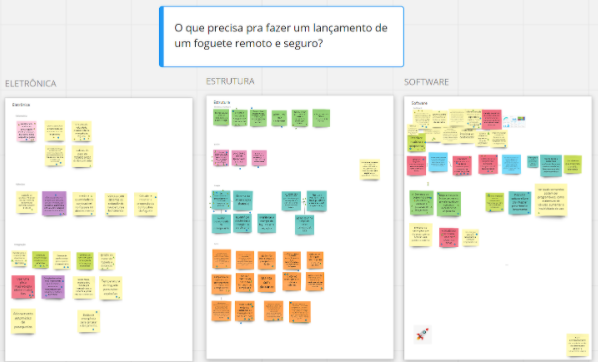
\includegraphics[scale=0.8]{figuras/miro.png}  
\caption{Brainwriting.}
\label{fig:miro}
\end{figure}

%\footnotesize Pode-se acessar em: \url{https://miro.com/app/board/o9J_kmVCAxA=/}

\subsubsection{\textit{Storyboard}}

\par Sob a perspectiva de modelos de desenvolvimento, já é comum o uso de histórias de usuários como um aspecto fundamental quando se trata de adotar o modelo \textit{eXtreme Programming}. A ideia consiste em fornecer uma visão de alto nível dos requisitos de um sistema, usadas como principal entrada de informações sobre estimativas e cronogramas, além de guiar a identificação de tarefas de desenvolvimento e conjunto de testes de aceitação (AMBLER, 2004). 

\par O \textit{storytelling} geralmente concentra-se em três linhas de pesquisas distintas: Geração, Interação ou Visualização das histórias \cite{pozzer}. Assim, nesta etapa do trabalho, a ênfase será na linha de construção que remete a forma como a história é gerada, ou seja, como se dá a elaboração da estrutura que irá guiar aspectos mais gerais, como personagens, ações, objetos e relacionamentos entre usuário e desenvolvedor para que essas especificações sejam geradas.

\par \textit{Storytelling} é um novo paradigma de entretenimento digital que está avançando a passos largos, com a criação de técnicas e ferramentas que permitem que histórias interativas possam ser criadas, visualizadas e guiadas com o auxílio do computador \cite{pozzer}.
Por fim, a “Exibição” trata a forma de representação gráfica da história, ou seja, a transformação das abstrações das estruturas internas dos personagens em ações realistas dentro de um espaço gráfico.

\par Contudo, \textit{storytelling} é mais do que um método baseado no ato de contar uma história. Tem como finalidade a captura e a transmissão de conhecimento de forma estruturada. A metodologia adotada pela equipe entrelaça conceitos de RUP e ágil, o que faz que o dinamismo e a relação com o \textit{stakeholder} sejam de fácil acesso e de muita troca de informações, tornando os requisitos mutáveis e adaptáveis à medida que o processo acontece.

\par Com base nesse contexto, o \textit{storytelling} tem como objetivo assegurar a construção das histórias de usuário com o intuito de prevenir e corrigir as falhas de comunicação e conceito de escopo que possam existir durante o processo.

\par O artefato que foi gerado pela equipe pode ser conferido nas Figuras \ref{fig:storytelling01} e \ref{fig:storytelling02}:

"\textit{Guto é um integrante de uma equipe de competição universitária de lançamento de foguetes de pequeno porte e comumente enfrenta problemas com o lançamento dos foguetes da equipe por conta da necessidade da execução manual  obrigatória de rotinas de lançamento.}
    
\textit{Além disso, as informações a respeito do lançamento e do desempenho do foguete são turvas e só podem ser obtidas após a recuperação do foguete, que acontece depois da competição.}

\begin{figure}[H]
\centering
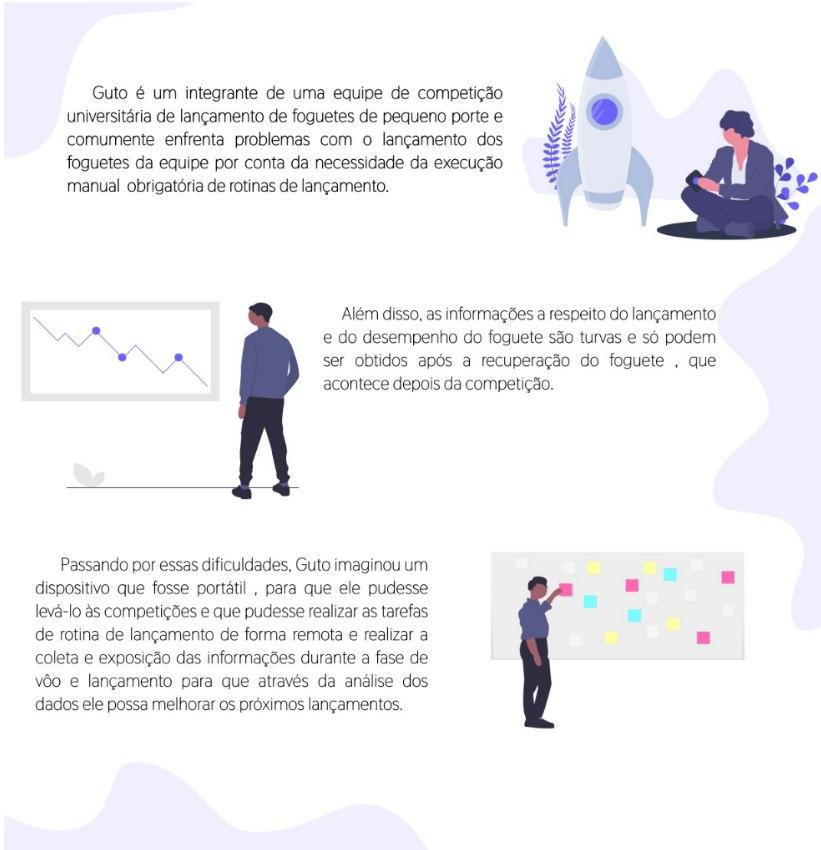
\includegraphics[width=0.8\textwidth]{figuras/storytelling1.jpg}
\caption{Storytelling: Página 1}
\label{fig:storytelling01}
\end{figure}

\textit{Passando por essas dificuldades, Guto imaginou um dispositivo que fosse portátil, para que ele pudesse levá-lo às competições, e que pudesse realizar as tarefas de rotina de lançamento de forma remota e realizar a coleta e exposição das informações durante a fase de vôo e lançamento para que através da análise dos dados ele possa melhorar os próximos lançamentos.}

\textit{Assim surgiu o  GCS , um dispositivo portátil, que, além de sanar as dificuldades de Guto, é portátil, seguro, e projetado por meio do método “user centered design”, para que as suas funcionalidades sejam intuitivas e de fácil usabilidade para o usuário.}

\begin{figure}[H]
\centering
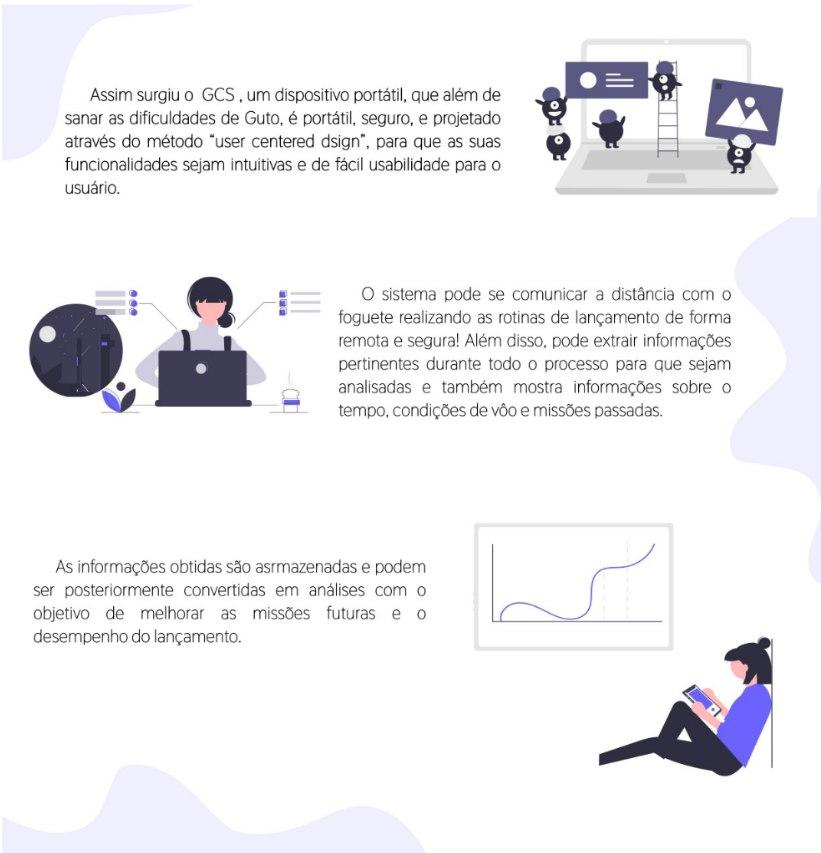
\includegraphics[width=0.9\textwidth]{figuras/sotytelling2.jpg}
\caption{Storytelling: Página 2}
\label{fig:storytelling02}
\end{figure}

\textit{O sistema pode-se comunicar à distância, com o foguete realizando as rotinas de lançamento de forma remota e segura! Além disso, pode extrair informações pertinentes durante todo o processo para que sejam analisadas e também mostra informações sobre o tempo, condições de voo e missões passadas.}"

\subsection{Arquitetura da informação}

\par A arquitetura da informação é a ciência de organizar e categorizar \textit{web sites}, intranets, comunidades \textit{online} e \textit{softwares}, para favorecer a usabilidade e a facilidade, para se encontrar o que se procura. Ou seja, é a estruturação de toda a informação disponível em um site ou aplicação, para que os usuários possam encontrar fácil e rapidamente o que procuram. E o arquiteto de informação é, na essência, o responsável por isso \cite{de2011fundamentos}. 

\par Durante a execução desta etapa do projeto, a equipe dedicou-se a executar atividades que fossem relacionadas aos princípios do \textit{User Centered Design}, e, com base nisso, à elaboração de artefatos que ajudassem a construir uma interface intuitiva para o usuário. Os artefatos elaborados pela equipe podem ser conferidos nas sessões seguintes.

\subsubsection{\textit{Wireframe}}

\par Os \textit{wireframes} são diagramas de baixa fidelidade que representam o layout de um site ou aplicação. A sua relevância no processo de \textit{design} deve‐se ao fato de permitirem explorar, testar e iterar ideias de \textit{design} numa fase inicial do projeto, momento em que as mudanças não vão aumentar o orçamento do trabalho. É importante que as pessoas responsáveis pela criação de conteúdo estejam envolvidas no processo de \textit{wireframing} \cite{brito2016usabilidade}. 

\begin{figure}[H]
\centering
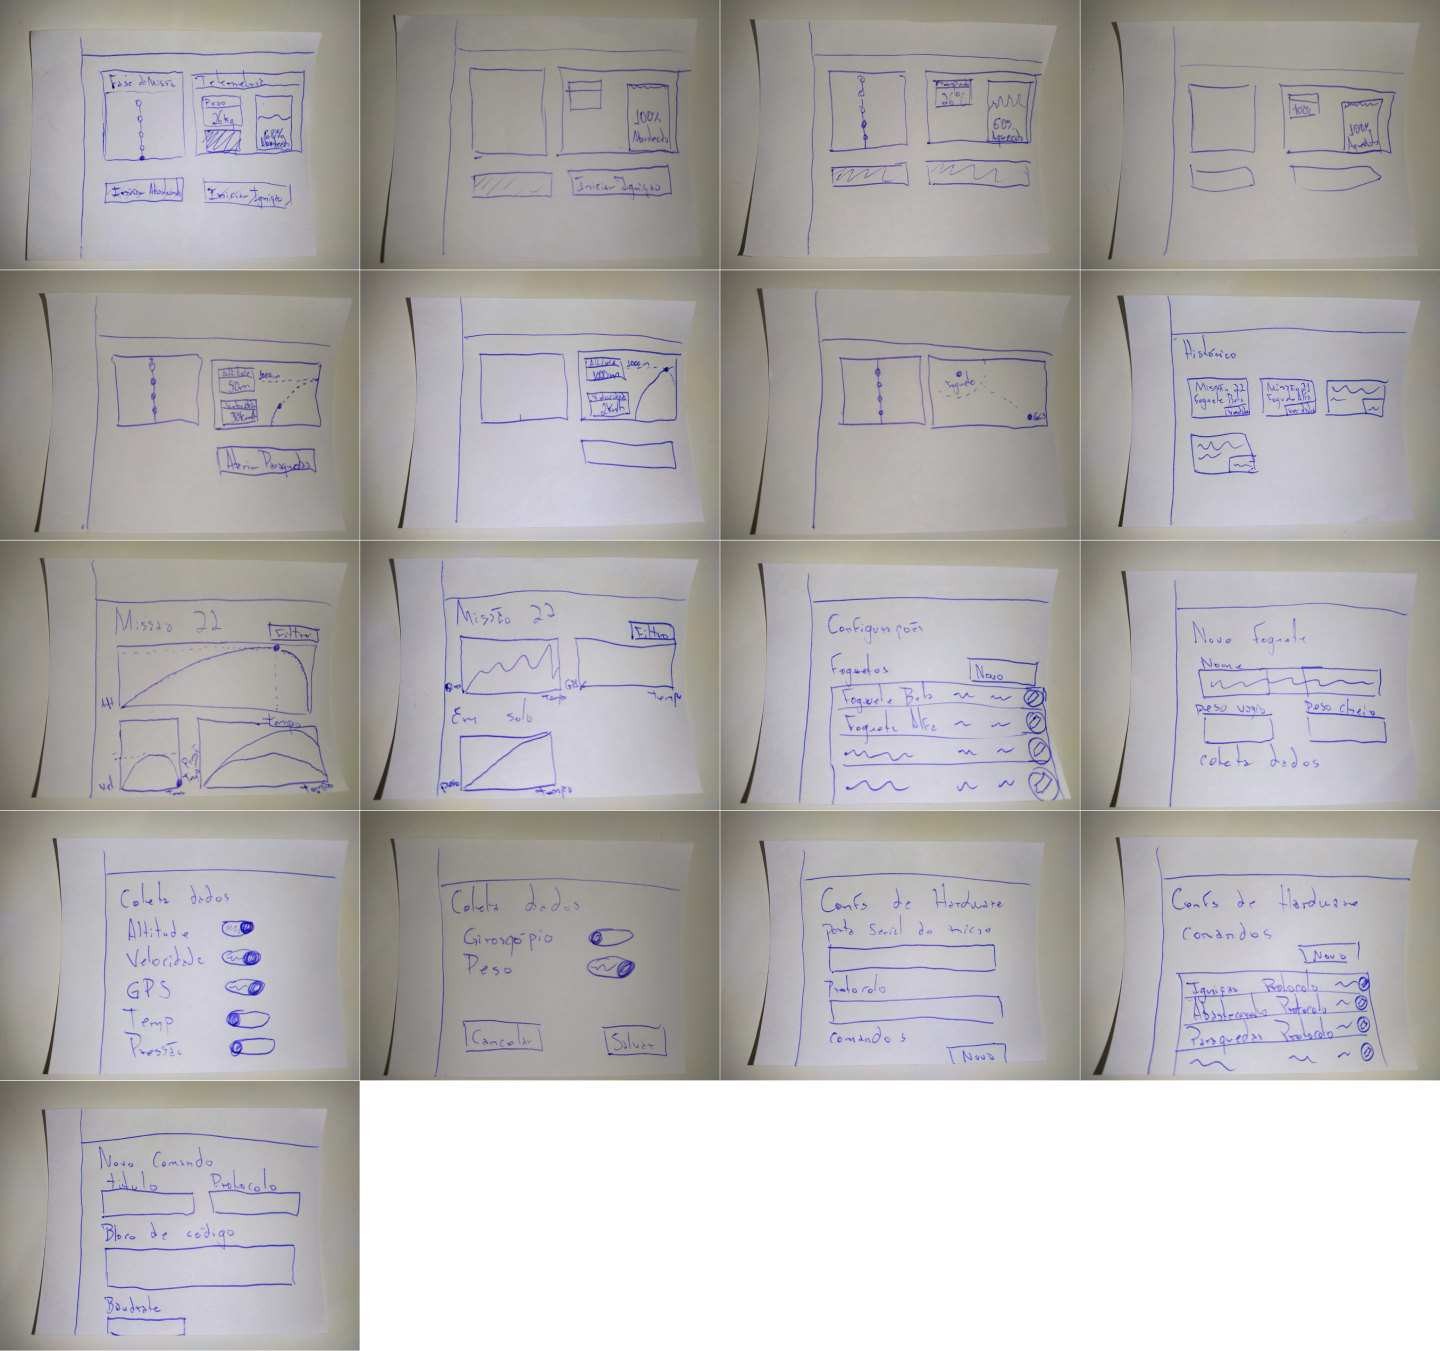
\includegraphics[scale=0.21]{figuras/wireframe.png}  
\caption{Wireframe}
\label{fig:Wireframe}
\end{figure}

\par Com o objetivo de testar as possíveis versões da interface e iterar a organização estrutural da informação da aplicação, a equipe elaborou um \textit{wireframe}, que foi validado com os usuários e \textit{stakeholders}. Esse artefato é apresentado na Figura \ref{fig:Wireframe} e também pode ser visualizado \href{https://bit.ly/3jnLnmN}{aqui}.


\subsubsection{Protótipo de média fidelidade}
\label{prototipo}

\par A prototipação no desenvolvimento de \textit{software} é um processo que tem como função avaliar as ideias geradas e validar – ou não – todos os requisitos estabelecidos \cite{lilley2004development}. É nesse momento que a equipe tende a  tirar as ideias do papel e passar a entendê-las na forma física.

\par Essa etapa é importante para verificar se a solução desenhada está adequada ao desafio que o cliente enfrenta, garantindo o alinhamento das informações. Dessa forma, consegue-se minimizar os riscos, permitindo que o cliente valide e faça todos os testes antes da implantação. É importante ressaltar que a fase de prototipação pode – e muitas vezes deve – ser realizada em diversos momentos, já que se verificam falhas de forma ágil, chegando assim a uma solução de software mais assertiva.

\par Apesar de já serem definidos diversos requisitos antes do desenvolvimento do \textit{software}, é durante a interação real do usuário com o sistema que os novos detalhes são percebidos. Para isso, a equipe realizou a elaboração de protótipos de baixa e média fidelidade, com a colaboração dos usuários e \textit{stakeholders}. As versões dos protótipos podem ser conferidas a seguir:


\href{https://bit.ly/35xe23N}{Protótipo V0}.

\href{https://bit.ly/2FW3oep}{Protótipo V1}.

\href{https://bit.ly/34pAfS2}{Protótipo V2}.

\subsection{Definição do produto}

\par O projeto aplica-se a um contexto de competições de lançamento de foguetes experimentais, onde cada equipe constrói seu foguete com base no regulamento da competição. Os projetos necessitam estar adequados o melhor possível às regras para obter uma boa pontuação. Devido à dinamicidade dos projetos e da baixa restrição de \textit{hardware} das competições, temos diversas configurações de \textit{hardware}. Nesse contexto, os sistemas de \textit{software} têm uma grande necessidade de adequação e adaptação aos diferentes \textit{hardwares} possíveis.

\par O produto de \textit{software} visa auxiliar o controle e monitoramento do lançamento de um foguete experimental para competições, provendo segurança, controle e visão de uma missão \footnote{Uma missão é todo o processo de lançamento de um foguete em uma competição. Vai desde a preparação para o abastecimento até a coleta do foguete após pousar.}. O sistema irá atuar em 3 momentos na competição:

\begin{itemize}
    \item abastecimento e ignição do foguete;
    \item foguete em voo;
    \item foguete em pouso.
\end{itemize}

\par Em ambos os momentos da competição, o sistema comunicar-se-á com \textit{hardwares} externos para fazer as leituras e enviar comandos de controles. Para tornar o produto de software valioso para os clientes, é fundamental satisfazer os objetivos e restrições expostos. Assim, faz-se necessária a construção de um sistema que permita a visualização e controle dos processos da missão, a partir de dados de telemetria e comandos para o \textit{hardware}, sendo estes configuráveis.Portanto, podemos definir as principais funcionalidades do sistema como:

\begin{itemize}
    \item Possibilitar a leitura e exposição dos dados de telemetria do foguete:
    \begin{itemize}
        \item GPS;
        \item Altitude;
        \item Velocidade;
        \item Temperatura;
        \item Pressão;
        \item Giroscópio;
        \item Peso (em solo); 
    \end{itemize}
    \item Possibilitar comandos de ignição, abastecimento e abertura do paraquedas;
    \item Possibilitar configuração dos comandos e protocolos necessários para se comunicar com diferentes \textit{hardwares};
    \item Armazenar os dados de maneira segura.
\end{itemize}

\subsubsection{Mapa de requisitos}

\begin{figure}[h!]
\centering
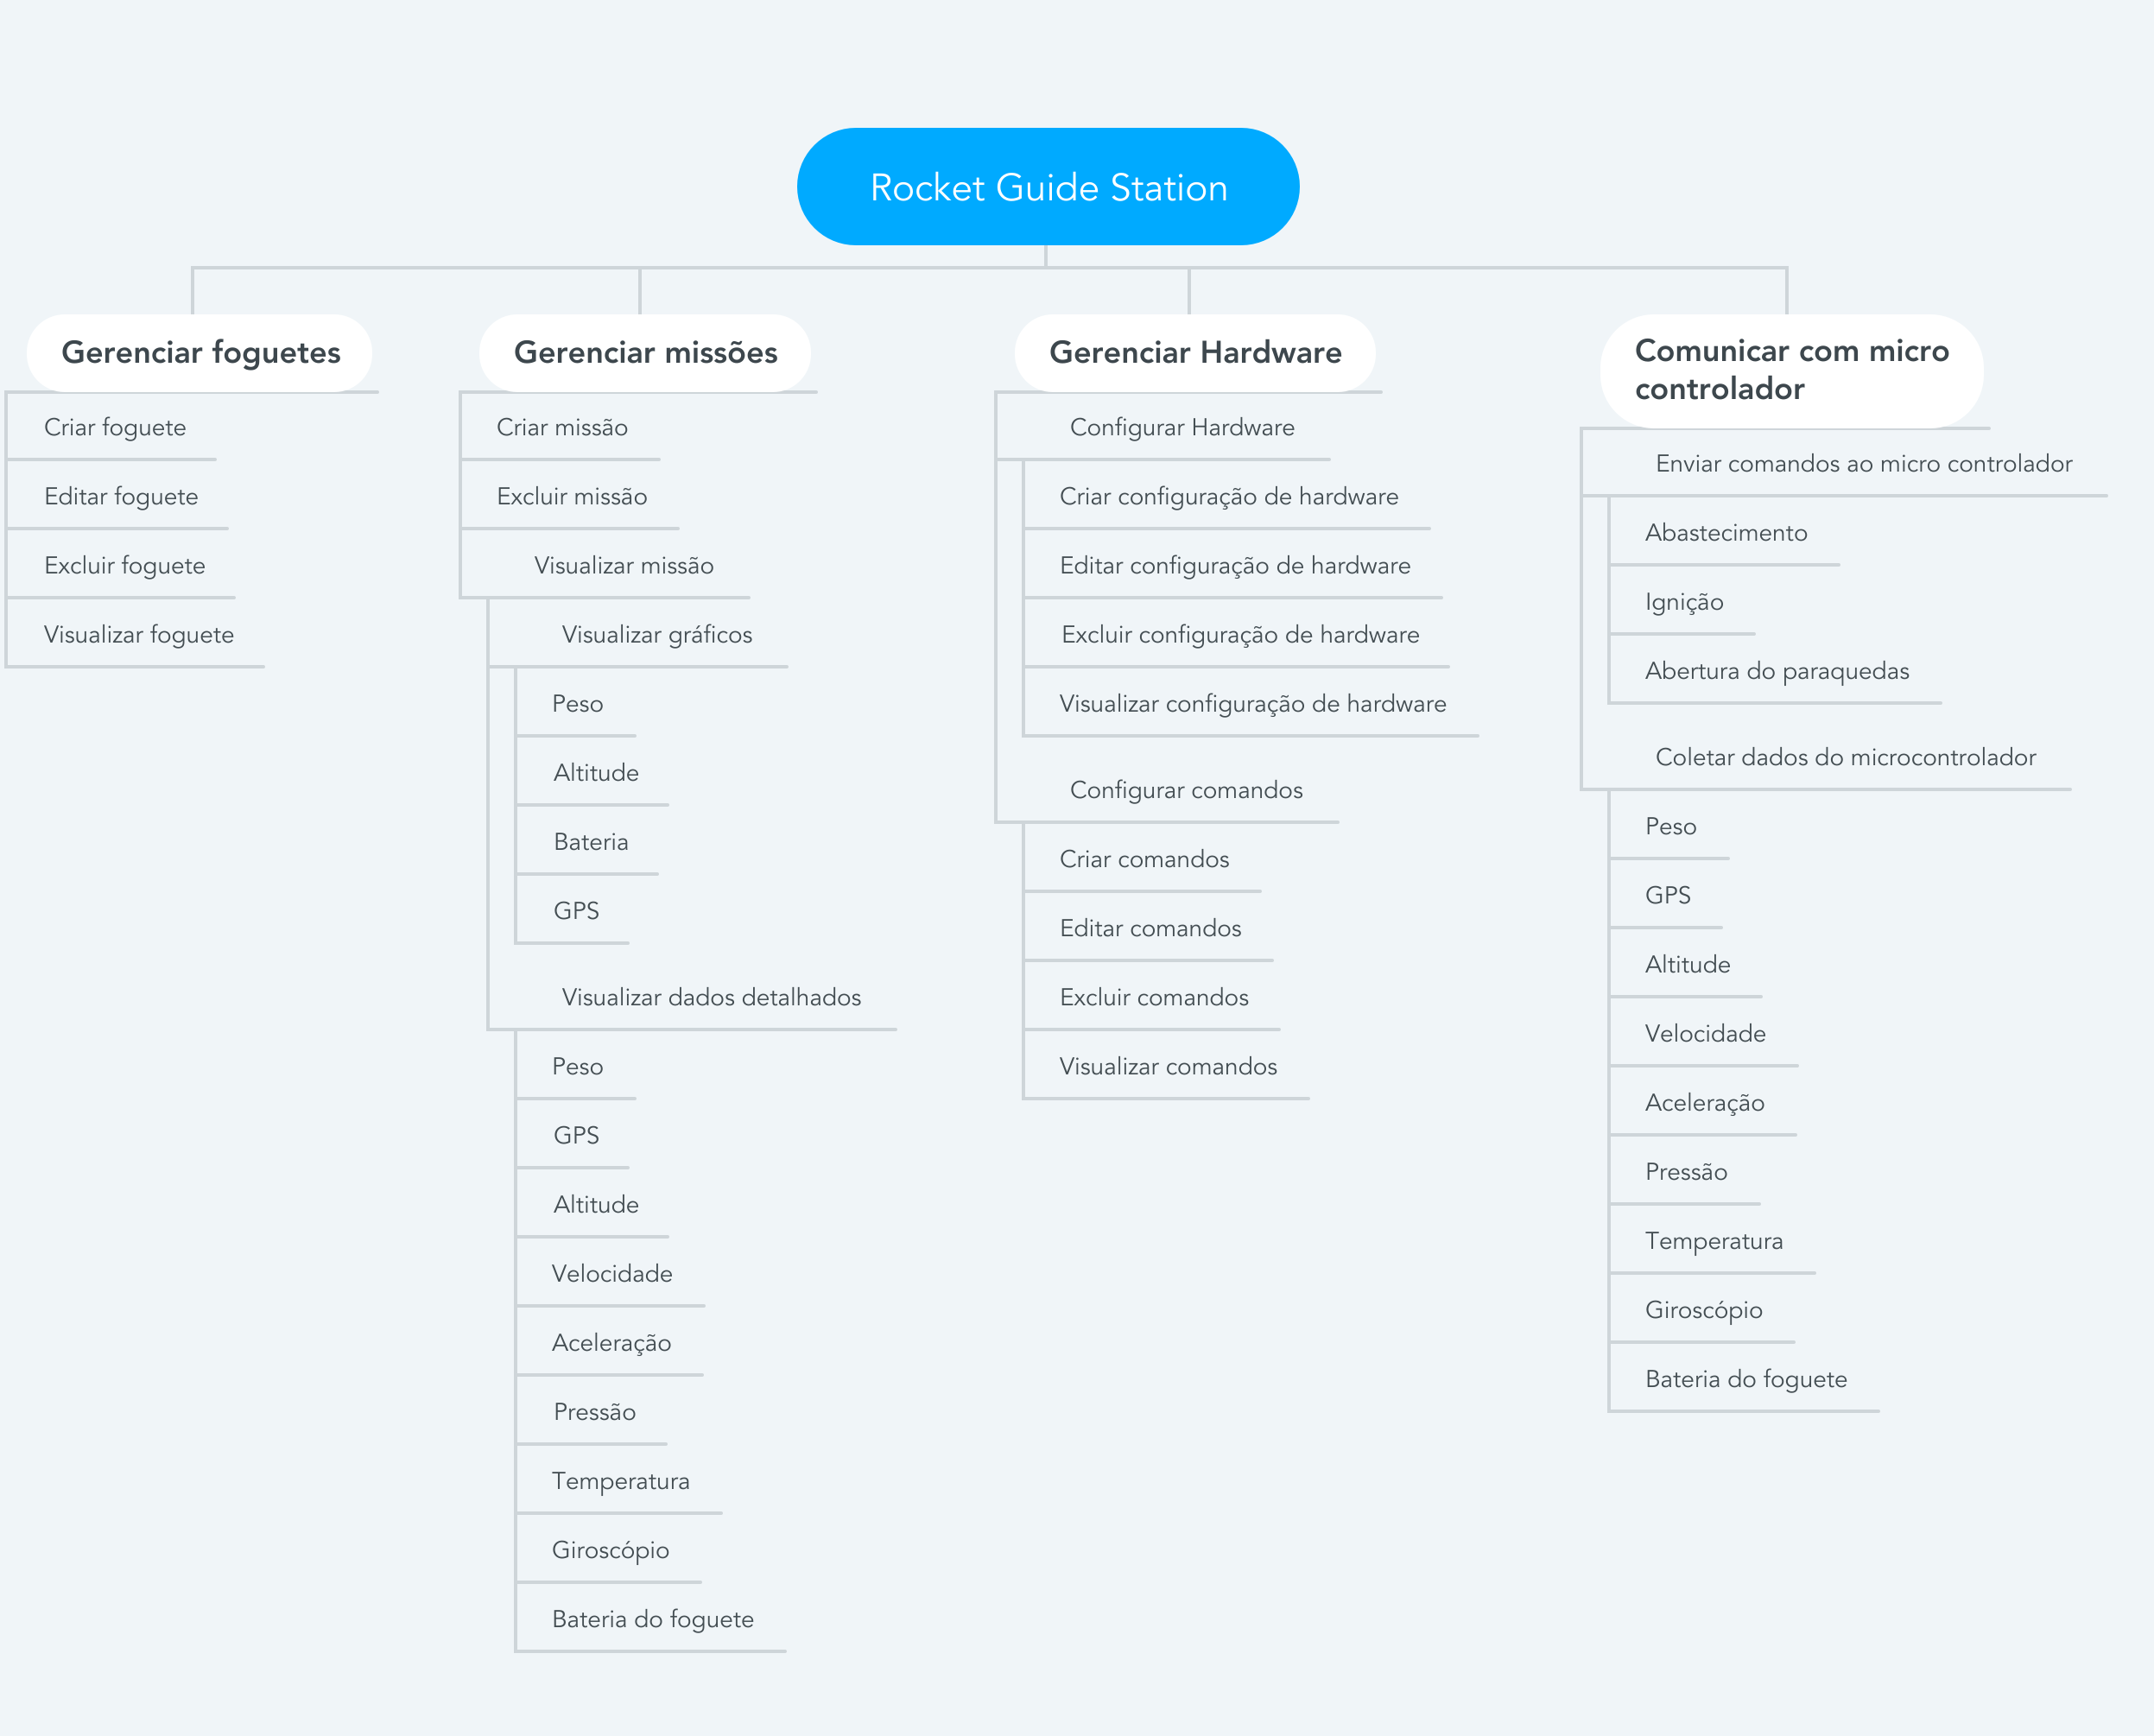
\includegraphics[scale=0.18]{figuras/Rocket_Guide_Station.png}  
\caption{Mapa de requisitos}
\label{fig:Mindmeister}
\end{figure}

\par Neste projeto, aplicamos técnicas de mapa mental para fazer a especificações de requisitos \cite{mapamental}. Utilizamos a ferramenta \textbf{Mind Meister} para construir o mapa mental. A partir da nova definição de produto, foi feito um mapa de requisitos demonstrando todos os requisitos do projeto. A Figura \ref{fig:Mindmeister} apresenta os épicos, ou principais funcionalidades: \textbf{Gerenciar Foguetes}; \textbf{Gerenciar Missões}; \textbf{Gerenciar Hardware}; e \textbf{Comunicar com o Micro Controlador}. Essas informações também estão disponíveis \href{https://mm.tt/1664123184?t=VJwmqWSqXf}{aqui}.




\section{Definição da Arquitetura}


%https://miro.com/app/board/o9J_kiYMRcI=/

\subsection{Padrão Arquitetural}

\par De acordo com o problema que o projeto visa resolver, a solução técnica proposta será embasada na arquitetura REST. A arquitetura \textit{Representational State Transfer} (REST), em português Transferência Representacional de Estado, é ideal ao nosso sistema, pois ele possui baixa complexidade e necessidade de utilização dos dados em tempo e estado definidos. De acordo com \cite{microservice} em suas conclusões, um sistema nem sempre se encaixa no perfil de um arquitetura distribuída, como a arquitetura micros-serviços, que, se aplicada de modo equivocado, pode prejudicar o bom andamento do projeto, pois exige maior complexidade no desenvolvimento e implantação do sistema, concluindo que esse tipo de arquitetura não deve ser aplicada a \textit{softwares} simples e com baixo grau de complexidade. 

\par A complexidade de um sistema nada diz sobre a eficiência e eficácia deste. Nossa solução proverá uma comunicação necessária para que as regras de negócio sejam aplicadas, satisfazendo as expectativas dos usuários e clientes. Após um estudo, foi verificado que uma \textit{Application Programming Interface} (API), em português Interface de Programação de Aplicativos, que seja RESTful, ou seja, capaz de implementar a arquitetura REST, é ideal para o problema proposto. 

\par No diagrama com protocolos de comunicação entre componentes do software, Figura \ref{fig:representacao_arq}, vemos que a comunicação entre os componentes do sistema deve ser planejada de maneira sistemática, e esse foi o caso. O sistema será construído usando a linguagem de programação JavaScript. O uso de JavaScript é bem comum para os \textit{browsers}, porém é necessários ajustes para a sua utilização a nível de \textit{backend}. Esses ajustes são realizados pelo \textit{runtime} Node.js, um ambiente em tempo de execução capaz de rodar um servidor \textit{web} local na porta 4200 como padrão. O Node.js, além de permitir a execução de código localmente fora no navegador, é responsável também por gerenciar pacotes e empacotar tudo que é necessário para executar e interpretar código JavaScript.

\par Na Figura \ref{fig:javascript backend} vê-se a lógica por trás da aplicação da linguagem \textit{JavaScript} em nossa API.

\begin{figure}[h!]
	\centering
	\label{javascript backend}
		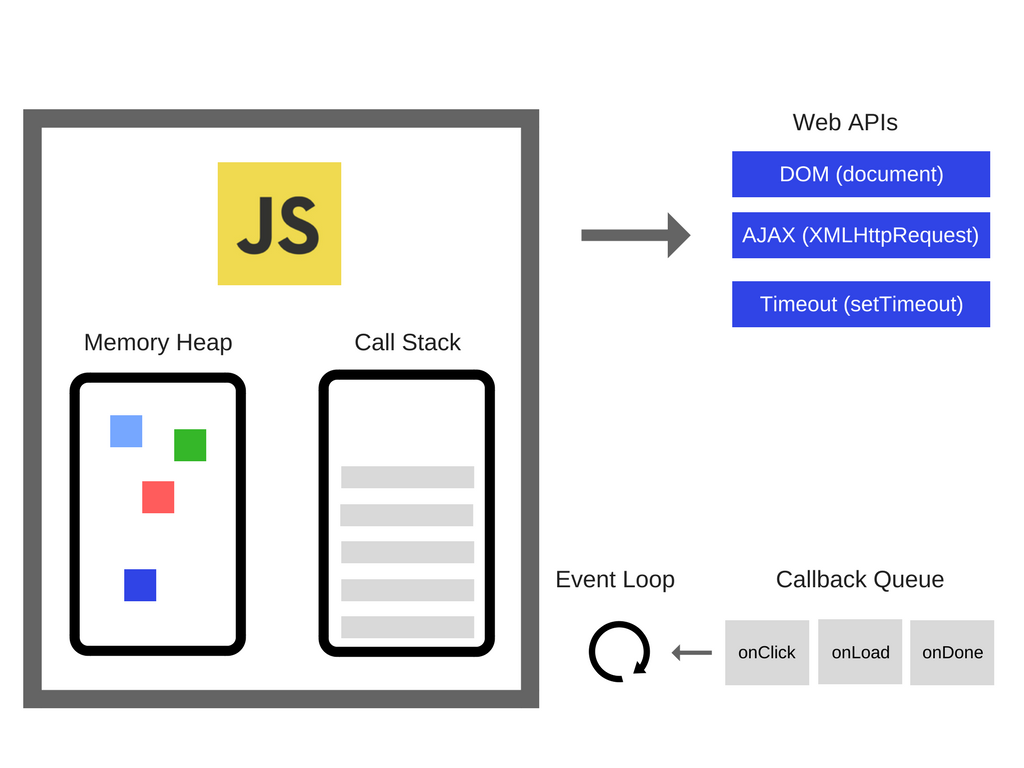
\includegraphics[keepaspectratio=true,scale=0.6]{figuras/javascript-backend.png}
	\caption{Modo como o JavaScript é executado fora do browser}
	{\footnotesize Fonte: \cite{javascript-backend}}
	\label{fig:javascript backend}
\end{figure}



\subsection{Representação da Arquitetura}

\begin{figure}[H]
\centering
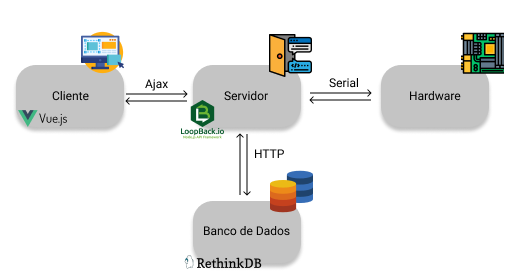
\includegraphics[width=0.9\textwidth]{figuras/representacao_arq.png}
\caption{Representação da Arquitetura}
\label{fig:representacao_arq}
\end{figure}


\subsubsection{Cliente}

\par Em aplicações \textit{web}, é muito comum adotar o conceito de \textit{Client-side} e \textit{Server-side} dentro da arquitetura em camadas \cite{ServerAndClient}. Nossa aplicação não será essencialmente \textit{web}, já que não será possível executar um \textit{browser} e também ter acesso à internet, assim como citado na Seção \ref{metas_restricoes} deste documento. Porém, vamos usar uma tecnologia inovadora implementada pelo \textit{framework} JavaScript Electron.js, que possibilita o desenvolvimento de aplicações \textit{desktop cross-platform}, em português seria algo como uma mescla de tipos de plataformas (\textit{web} e \textit{desktop}), utilizando ferramentas \textit{web} como JavaScript, HTML e CSS \cite{electron}.

\par O ciclo de vida do lado do Cliente (\textit{Client-side}) é representado na Figura \ref{fig:client-side}. O JavaScript faz requisições, ações que o usuário deseja executar ao utilizar a interface da aplicação, por meio de chamadas AJAX (Asynchronous JavaScript And XML), em português seria algo como JavaScript assíncrono + XML \cite{Ajax}. Com essa tecnologia, uma aplicação \textit{web} é capaz de realizar atualizações incrementais na interface apresentada ao usuário.

\begin{figure}[!h]
	\centering
		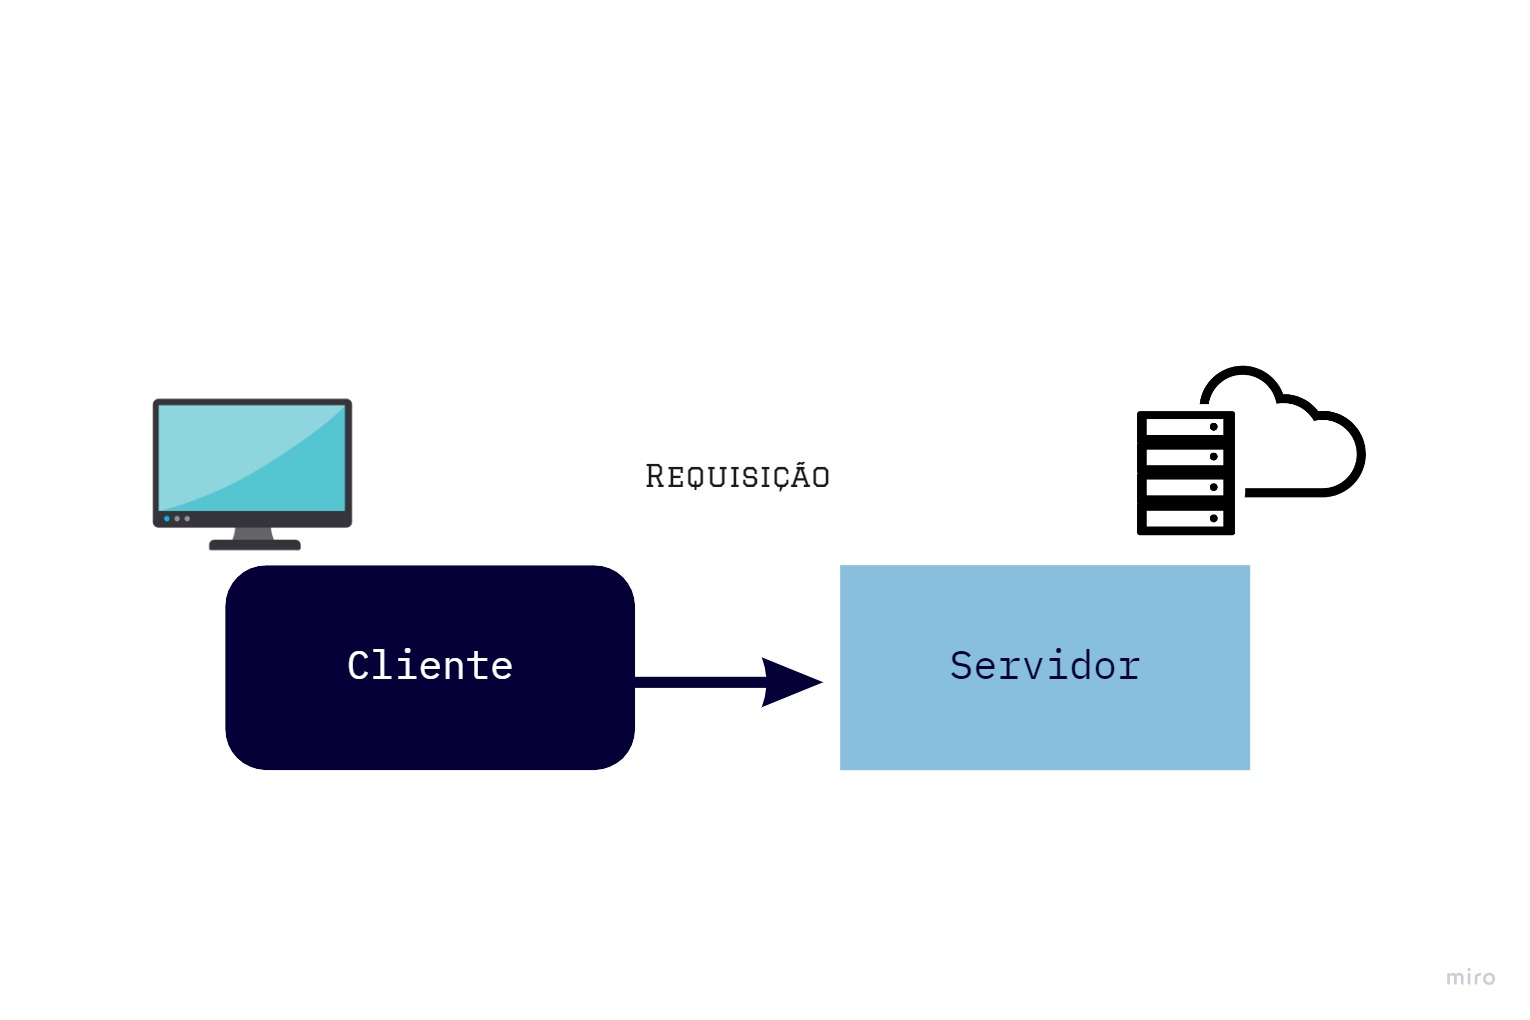
\includegraphics[keepaspectratio=true,scale=0.26]{figuras/client.jpg}
	\caption{Cliente da aplicação Desktop}
	\label{fig:client-side}
\end{figure}


\par A tecnologia que será usada é o Vue.js um \textit{progressive framework}, em português "\textit{framework} progressivo", em JavaScript para o desenvolvimento no \textit{Client-side} \cite{Vue} e também fazendo uso do "axios" que é um cliente HTTP baseado em \textit{promises}, que é um objeto usado para processamento assíncrono \cite{Promise}. Nesse contexto, o desenvolvimento \textit{frontend} será responsável por criar a interface gráfica e também a comunicação entre \textit{Client-side} e \textit{Server-side}. 

\subsubsection{Servidor}

\par Do lado do servidor, \textit{Server-side} Figura \ref{fig:Server-side}, temos recebimento de requisições por parte do cliente, o processamento lógico e, por fim, o envio da resposta correspondente ao cliente. 

\begin{figure}[H]
	\centering
		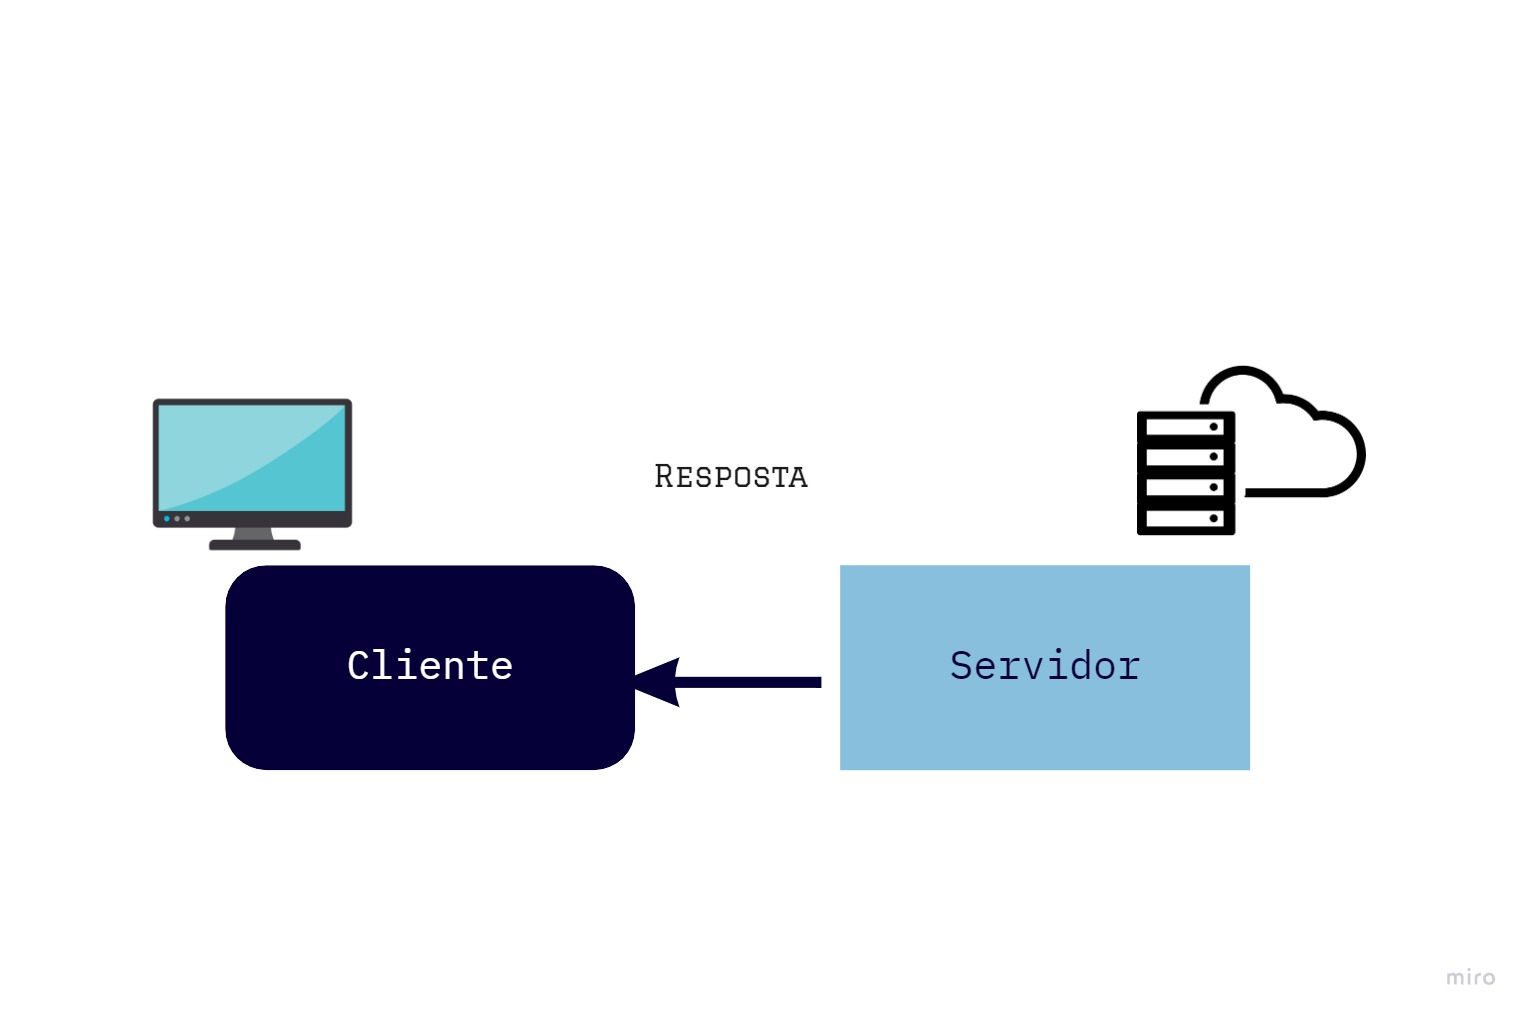
\includegraphics[keepaspectratio=true,scale=0.26]{figuras/server.jpg}
	\caption{Servidor da aplicação Desktop}
	\label{fig:Server-side}
\end{figure}

\par Faremos uso de uma API Rest escrita em JavaSript, por meio do Framework Loopback, um \textit{framework} altamente expansível baseado no famoso Express e em Node.js + Typescript \cite{Loopback}. Dessa forma, poderemos criar serviços REST que serão consumidos pelo Cliente por meio de \textit{endpoints}.

\par Para o \textit{pipeline} de funções que manipulam as requisições e respostas HTTP que serão necessárias para a comunicação com o Banco de dados, faremos o uso de \textit{middleware}. Esse tipo de metodologia de processamento implementa o padrão de projeto \textit{Chain of Responsability}  \cite{Chain}, o qual é desenhado para desacoplar o envio e recebimento de mensagens dividindo a tarefa de manipulá-las entre múltiplos objetos tal como na Figura \ref{fig:chain-of-responsibility}.

\begin{figure}[H]
	\centering
	\label{chain-of-responsibility}
		
\includegraphics[keepaspectratio=true,scale=0.22]{figuras/chain-of-responsibility.png}
	\caption{Padrão de Projeto Chain of Responsability \cite{ChainFigura}}
	\label{fig:chain-of-responsibility}
\end{figure}

\par Com o \textit{Loopback}, podemos criar uma sequencia de funções que realizam o processamento adequado de mensagens conforme representado na Figura \ref{fig:middleware} \cite{Loopback}.

\begin{figure}[H]
	\centering
	\label{middleware}
		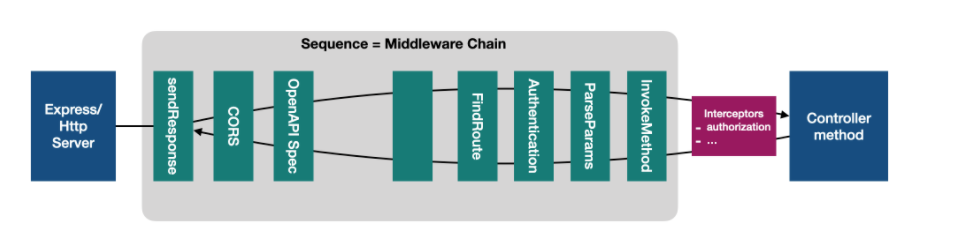
\includegraphics[keepaspectratio=true,scale=0.75]{figuras/middleware.png}
	\caption{Sequência baseada em Middleware  \cite{Loopback}}
	\label{fig:middleware}
\end{figure}


\subsubsection{Banco de Dados}

\par Para oferecer uma experiência satisfatória ao usuário da aplicação, os dados devem ser apresentados em tela em tempo real. Nossa base de dados deve ser capaz de detectar qualquer mudança realizada em seu armazenamento. Para isso, optamos por usar a tecnologia do banco de dados RethinkDB, um banco de dados \textit{open-source} capaz de realizar envio de dados no formato JSON em tempo real. 

\par Além disso, é um banco de dados NoSQL, que nos permite flexibilidade se comparado com bancos SQL, mas que mantém a organização a nível de modelagem de dados. A tecnologia por trás disso é a \textit{schemaless JSON documents}, um armazenamentos de documentos JSON não esquematizado.Todos os documentos NoSQL armazenam suportam as mesmas operações básicas:

\begin{itemize}
    \item criar ou apagar registros de uma coleção;
    \item criar, recuperar, atualizar ou deletar um documento;
    \item consultar uma coleção;
    \item criar ou apagar registros de índices. 
\end{itemize}

\par Dessa forma, teremos uma ferramenta poderosa para manipular nossos dados.Diferentemente de bancos SQL, os arquivos são escritos em documentos, com estruturas semelhantes às Figuras \ref{fig:json} e \ref{fig:xml}.

\begin{figure}[!h]
	\centering
	\label{json}
		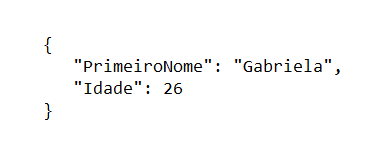
\includegraphics[keepaspectratio=true,scale=0.9]{figuras/json.png}
	\caption{Documento em formato JSON}
	\label{fig:json}
\end{figure}

\begin{figure}[!h]
	\centering
	\label{xml}
		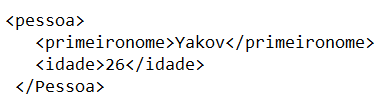
\includegraphics[keepaspectratio=true,scale=0.9]{figuras/xml.png}
	\caption{Documento em formato XML}
	\label{fig:xml}
\end{figure}

\subsubsection{\textit{Hardware}}

\par A comunicação entre o \textit{hardware} e o \textit{software} do projeto é feita via porta serial. Em fase experimental, iremos fazer um \textit{script} para simular o funcionamento dessa integração e relatar o desempenho possível e desejado. Até o momento, não foram encontradas evidências de que o \textit{script} não poderá ser escrito em JavaScript, já que existe a biblioteca Serialport.js \cite{serialport} que dá o necessário suporte a esse tipo de comunicação. Porém, caso haja qualquer problema de compatibilidade, faremos uso do padrão de projeto Adaper, que tem como objetivo prover uma interface que liga objetos com diferentes tipos de linguagem e protocolos de comunicação. O padrão é representado pela Figura \ref{fig:adapter}.

\begin{figure}[!h]
	\centering
	\label{adapter}
		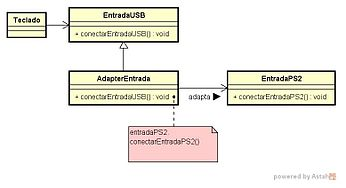
\includegraphics[keepaspectratio=true,scale=1]{figuras/adapter.jpg}
	\caption{Padrão de projeto Adapter \cite{Adapter}}
	\label{fig:adapter}
\end{figure}

\subsection{Ambiente}

\par Tendo em vista a arquitetura do projeto e a falta da placa para testar o sistema nas condições reais, foi adotada a estratégia de conteinerização dos serviços. Assim é possível isolar os ambientes, bem como facilitar a configuração do ambiente de produção (já embarcado no dispositivo). Para isso, foram utilizadas as seguintes tecnologias:

\begin{itemize}
    \item Docker \cite{docker}
    \item Docker - Compose \cite{docker-compose}
\end{itemize}

\subsection{Arquitetura computacional}

\par O sistema será desenvolvido para ser executado em um computador de arquitetura 64 bit ARM (Arm64) e um sistema operacional que opere nessa mesma arquitetura \cite{arquitetura_arm}.

\section{Diagrama de Sequência}

\par O principal objetivo do diagrama de sequência é verificar se ele é consistente com a declaração dos requisitos, bem como com sua estrutura de árvore bem formada. Enquanto isso, a construção do diagrama é definida em termos das transições de estado, que são realizadas pelas invocações de método no diagrama, representados no nosso contexto por Cliente, Servidor, Banco de Dados e Micro Controlador. Quando uma mensagem é executada, ela deve ser consistente com o estado do sistema, e com as dependências de transações entre os estados \cite{li2004formal}.

\par Para garantir um alinhamento e uma comunicação de qualidade com os componentes de eletrônica, esse diagrama foi evoluído para garantir a documentação e a estruturação da comunicação entre os times. A Figura \ref{fig:Diagrama_sequencia_missao_1} apresenta a fase de missão, onde o usuário solicita o início da ignição à camada da interface, que por sua vez, solicita ao servidor (camada da API), que consulta o comando a ser enviado ao hardware no banco de dados, e ao obter essa informação envia o comando. Após receber o comando e iniciar o processo, o sistema receberá uma confirmação do início. Após confirmar o início do processo de ignição, é realizada a troca da comunicação que antes era feita com o microcontrolador da base e que agora será feita com o do foguete, para receber as informações do voo. A atualização das informações para o usuário é iniciada em um loop, como apresentado no Apêndice \ref{diagrama_sequencia}, Figura \ref{fig:Diagrama_sequencia_missao}. Que apresenta o loop que é executado durante todo o processo para coletar as informações dos sensores e armazenar no banco de dados. As Figuras \ref{fig:Diagrama_sequencia_cadastr_foguete}, \ref{fig:Diagrama_sequencia_cadastro_micro}, \ref{fig:Diagrama_sequencia_missao}, \ref{fig:Diagrama_sequencia_abastecimento}, \ref{fig:Diagrama_sequencia_desengate}, \ref{fig:Diagrama_sequencia_ignicao}, \ref{fig:Diagrama_sequencia_finaliza_missao}, \ref{fig:Diagrama_sequencia_historico} apresentam respectivamente o processo de lançamento do foguete pela estação desenvolvida.

\begin{figure}[htb]
    \centering
    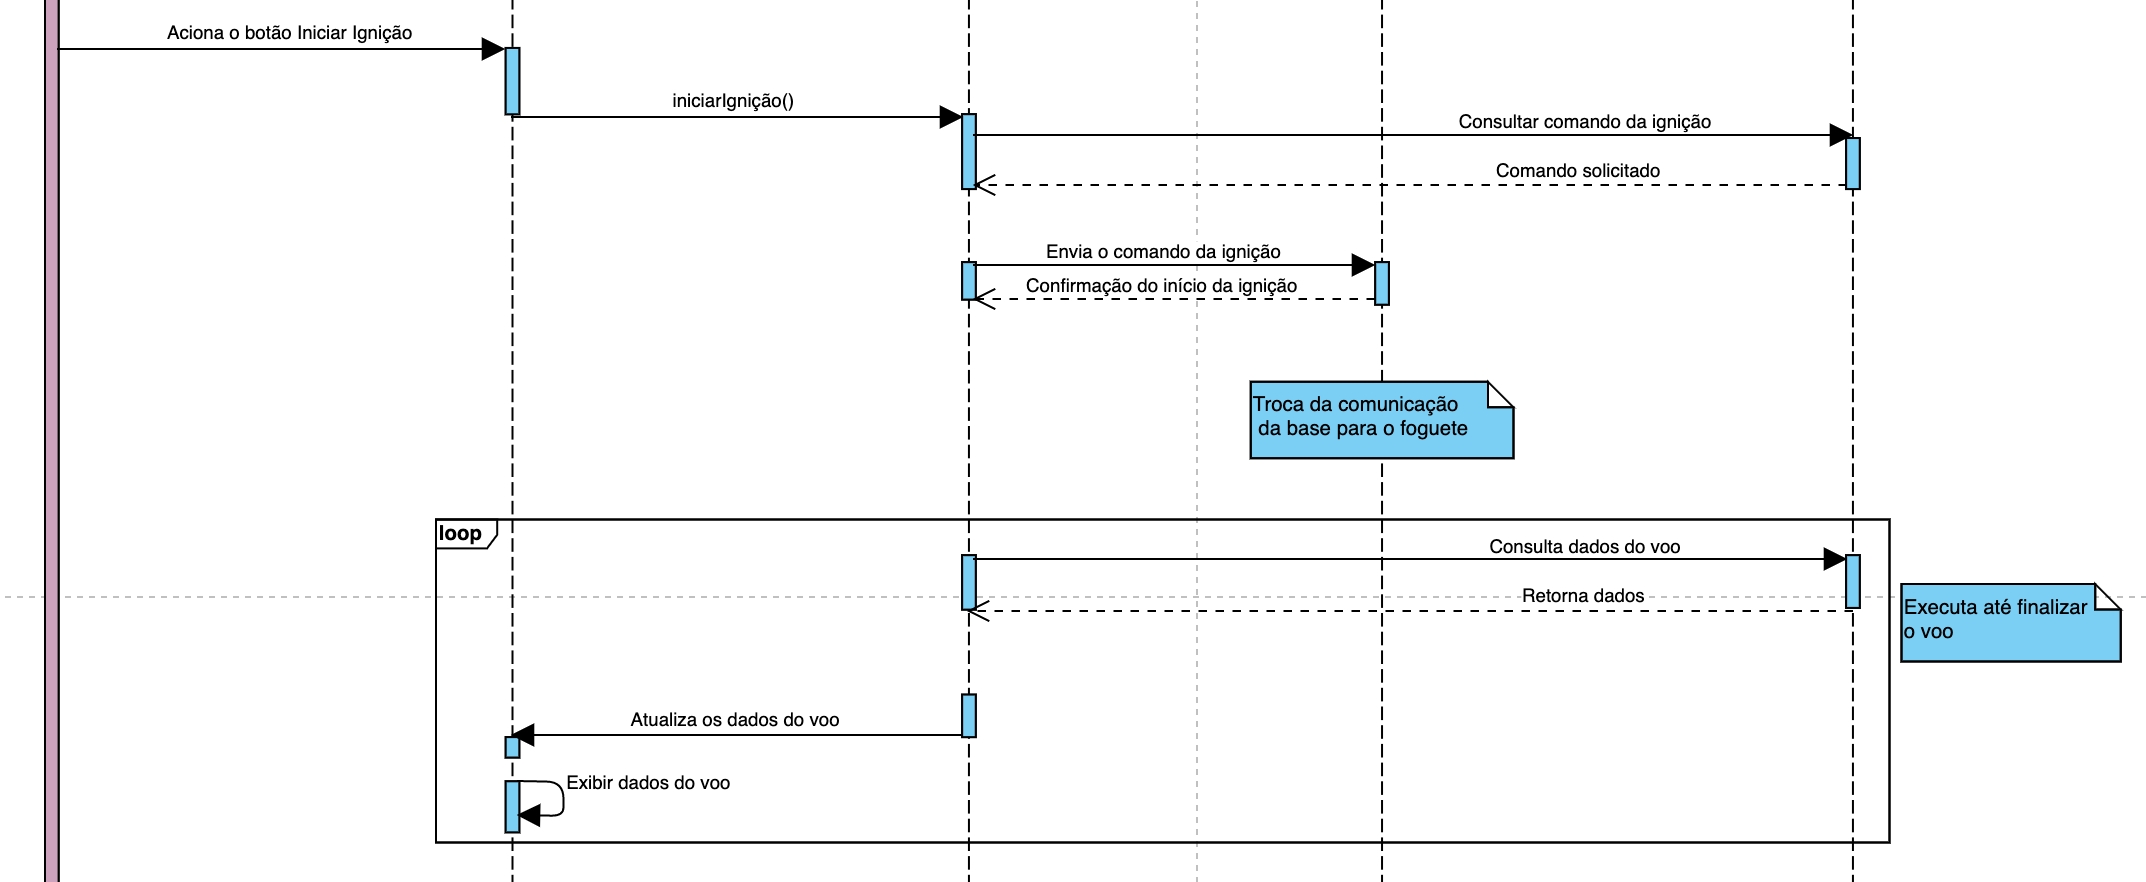
\includegraphics[width=1\textwidth, angle=0]{figuras/diagrama_sequencia_ignicao.png}
    \caption{Diagrama de sequencia representando o processo da ignição do foguete. Fonte: Autor}
    \label{fig:Diagrama_sequencia_missao_1}
\end{figure}

\par Nós construímos o diagrama de sequência, presente no Apêndice \ref{diagrama_sequencia}, com o objetivo de alinhar o processo de lançamento e especificar os requisitos.

\section{Modelagem de Dados}

\par A modelagem dos dados foi feita com base nos requisitos e utilizando o \textit{software} BrModelo. Primeiro, optamos por fazer o modelo conceitual especificar em um nível mais alto as entidades e seus relacionamentos. A Figura \ref{fig:conceitual} apresenta as entidades: \textbf{Foguete, Missão, Temperatura, Velocidade, GPS e Pressão}, mantendo um relacionamento. As entidades \textbf{Hardware e Comando} não possuem relação com a entidade Foguete e Comando, pois se trata de uma configuração presente na \textit{Ground Station} apenas, não interagindo assim diretamente na Missão e no funcionamento do Foguete.

\begin{figure}[h!]
	\centering
		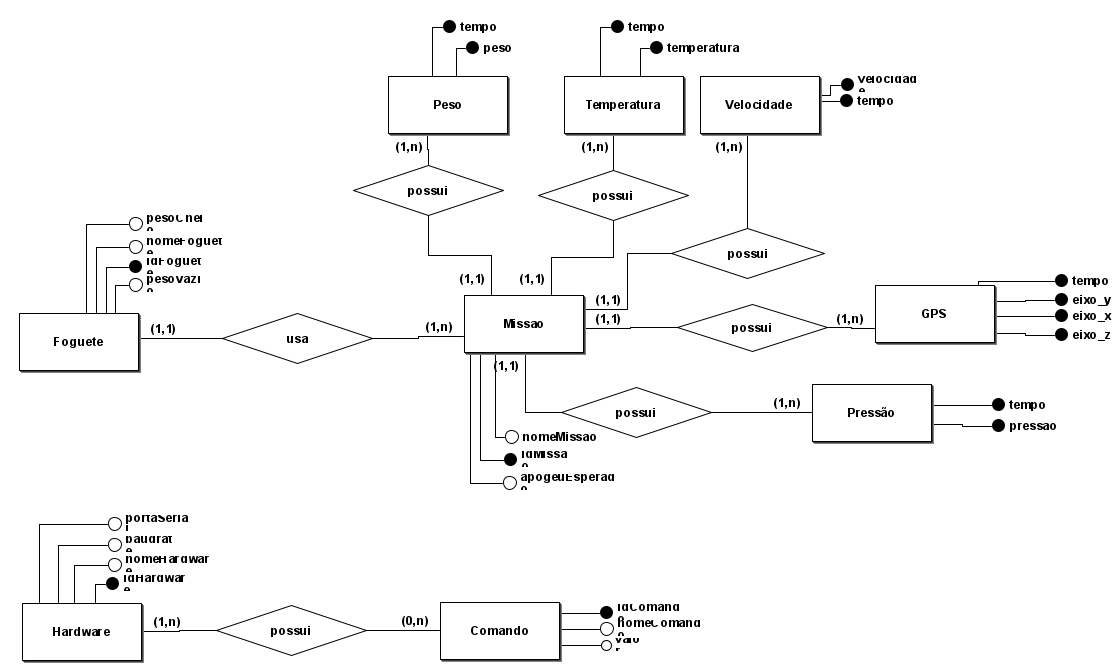
\includegraphics[keepaspectratio=true,scale=0.4]{figuras/conceitual_ground_station.png}
	\caption{Modelo Conceitual da modelagem.}
	\label{fig:conceitual}
\end{figure}


\begin{figure}[h!]
	\centering
		\includegraphics[keepaspectratio=true,scale=0.4]{figuras/Lógico_ground_station.png}
	\caption{Modelo Lógico da modelagem}
	\label{fig:logico}
\end{figure}

\par Em seguida, foi gerado o modelo lógico da implementação para representar as tabelas junto com as chaves primarias e estrangeiras. A Figura \ref{fig:logico} apresenta essa implementação.

\section{Diagrama de Pacotes}
A Figura \ref{fig:diagrama_pacote_backend} apresenta o diagrama de pacotes do backend do projeto. Ele contem a estrutura de pastas utilizada para o desenvolvimento utilizando loopback4.js. Essa estrutura apresenta as pastas e as relações entre elas para a o funcionamento do projeto.
\begin{figure}[h!]
	\centering
		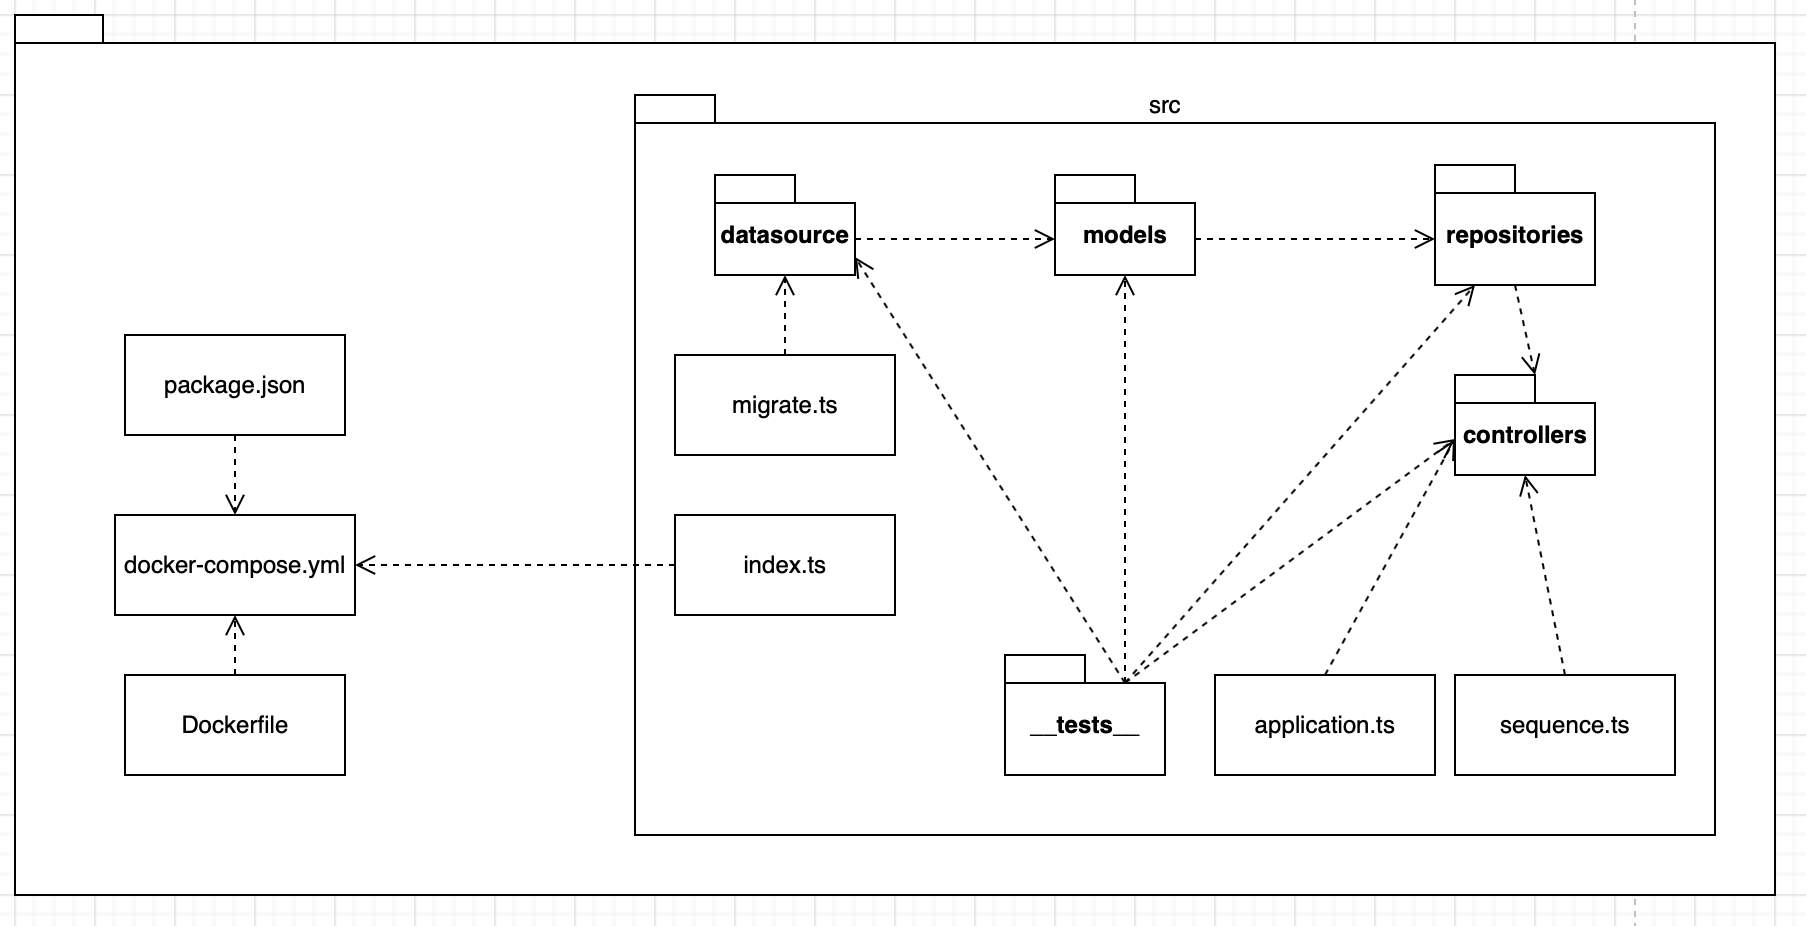
\includegraphics[keepaspectratio=true,scale=0.4]{figuras/diagrama_pacotes_backend.png}
	\caption{Diagrama de representação dos pacotes e as relações do Back end}
	\label{fig:diagrama_pacote_backend}
\end{figure}

A Figura \ref{fig:diagrama_pacote_frontend} apresenta a organização de pacotes do front end a partir de um diagrama de pacotes. O Vue.js é organizado de uma forma em que os arquivos das \textit{Views} e das \textit{Models}, representado pela pasta \textit{Store}. Além disso, o Vue permite a criação de componentes, que ficam armazenados na pasta \textit{Components} e podem ser utilizados em páginas das \textit{Views}.
\begin{figure}[h!]
	\centering
		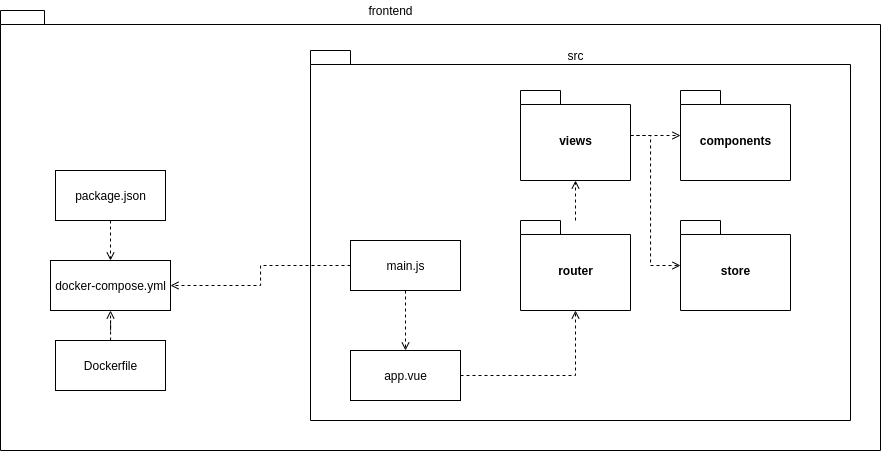
\includegraphics[keepaspectratio=true,scale=0.4]{figuras/diagrama_pacotes_frontend.png}
	\caption{Diagrama de representação dos pacotes e as relações do Front end}
	\label{fig:diagrama_pacote_frontend}
\end{figure}

\section{Metas e restrições de arquitetura}
\label{metas_restricoes}

\subsection{Metas}

\begin{itemize}
    \item Auxiliar o usuário no lançamento e acompanhamento de voo de um foguete experimental.
    \item Armazenar dados dos lançamentos de forma sistemática.
    \item Ter uma interface intuitiva e de fácil utilização, para agilizar o processo de lançamento do foguete e análise dos dados pós voo.
    \item Possibilitar o controle do lançamento e acompanhamento do voo do foguete.
\end{itemize}

\subsection{Restrições}

\begin{itemize}
    \item O sistema não terá acesso a internet.
    \item Deve ser executado em microcomputador com recursos limitados.
    \item Realizar  \textit{streaming} de dados obtidos do foguete em tempo de execução.
    \item Disponibilizar dados armazenados em CSV para exportação via cartão SD.
    \item Utilizar ambiente conteinerizado, Docker, para virtualização do ambiente, a fim de poder simular o comportamento do software, já que não teremos a placa para fazer os testes.
    \item Deve ser utilizado um computador de arquitetura 64 bit ARM, Arm64, e um sistema operacional compatível.
\end{itemize}

\section{Inovação}
Como proposta de inovação, foi definida pela equipe, que o produto seria construido com base na metodologia do \textit{User Centered Design}. Por isso, todo o processo de elaboração e construção do produto, dês da sua ideação até a sua execução foram pautados nas regras da metodologia, e com base a equipe se aprofundava na obtenção de conhecimentos relacionados ao tema, os documentos iam sendo elaborados , revisados e refinados.

\section{Descrição do problema e proposta de inovação}

O User Centered design é o processo que foca nas necessidades e desejos dos usuários para o desenvolvimento de serviços ou produtos. A aplicação consistente de fatores humanos, ergonomia, usabilidade e outras técnicas é o que permite envolver os usuários no processo de elaboração do produto, junto á equipe de desenvolvimento.

O objetivo disso é criar sistemas altamente úteis e acessíveis, apontando na direção da satisfação dos usuários, evitando efeitos negativos na performance. É colocar cada pessoa para a qual o produto foi destinado no coração da experiência.

Comumente, os produtos de estações de controle terrestres são sistemas que são construidos visando tecnicidade e com pouco foco nas demandas reais dos usuários e pouca customização para cada caso específico.Assim, o design focado no cliente pode não apenas fornecer resultados reais e mensuráveis, mas também proporcionar uma vantagem competitiva diferenciada para o produto, pois foca em ter as necessidades específicas de um nicho de usuário sanadas, baseado em suas demandas em uma construção conjunta.

\subsection{Como executar um design de produto centrado no usuário}

O processo de construção de um user centered design se divide basicamente nas quatro fases a seguir:

\begin{itemize}
    \item Análise: Essa é  a fase de pesquisa, com análise de stakeholders, competidores, desenvolvimento de personas, definição de cenários de uso, condução de estudos de campo e definição de objetivos de usabilidade. 
    \item Design: Durante o design são criados modelos de navegação, fluxos de tela, arquitetura da informação, protótipos, wireframes, design de interação (ui design) e feitos alguns testes de usuário. Todos esses processos se utilizam das informações coletadas na análise para serem feitos pensando no usuário.
    \item Implementação : Durante a implementação, é finalizado o design orientado à objetos, a integração de interfaces de design, implementação de servers e realizada constante validação com os usuários.
    \item Desenvolvimento: A parte final é a parte do desenvolvimento, onde a avaliação contínua e valudação com o usuário se transformam em produto a partir das soluções identificadas nas fases anteriores. Nessa etapa, percebe-se a importância de uma construção de produto transparente e objetiva, para que o produto desenvolvido esteja o mais próximo possível do idealizado. 
\end{itemize}

A Figura \ref{fig:ucer_centered_design_fig} apresenta o processo de ciclo de vida da metodologia User Centered Design. As etapas subsequentes foram adotadas pela equipe e ajustadas de acordo com as demandas do projeto. 

\begin{figure}[h!]
	\centering
		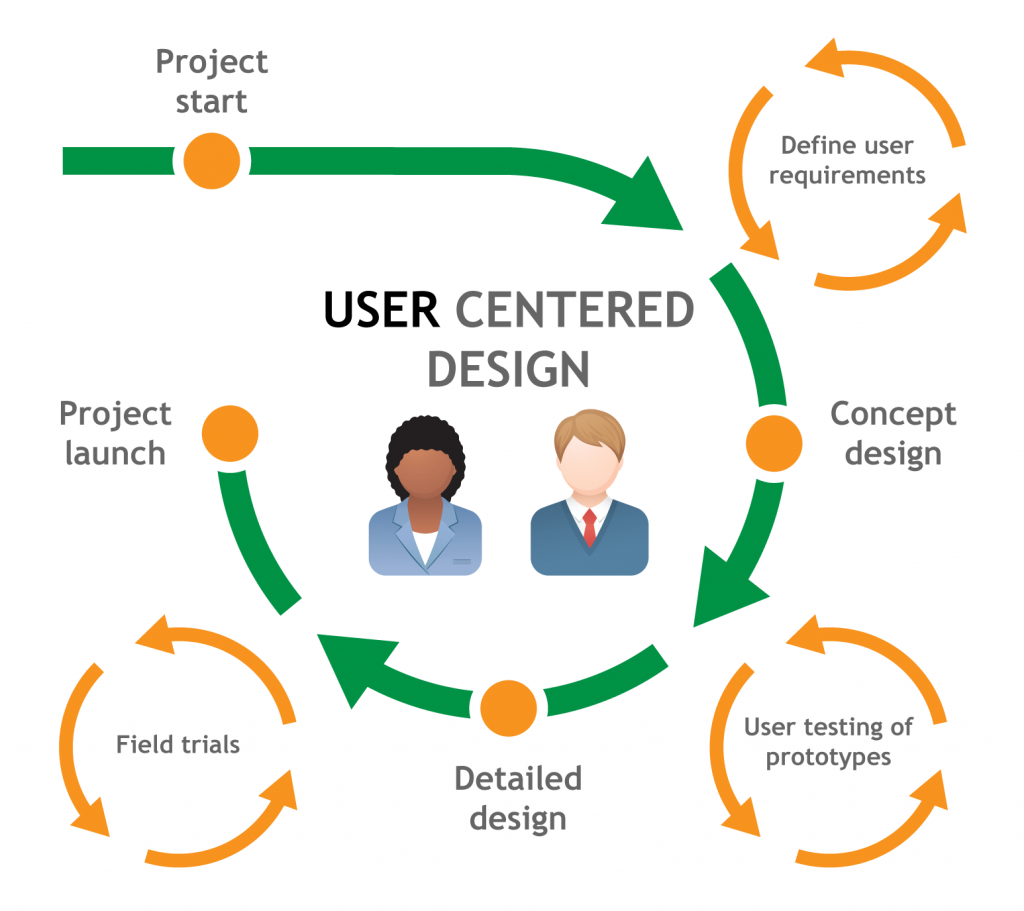
\includegraphics[keepaspectratio=true,scale=0.4]{figuras/UserCentered.png}
	\caption{Ciclo de vida do User Centered Design}
	\label{fig:ucer_centered_design_fig}
\end{figure}

\section{Construção Front end}

A construção do Front end foi desenvolvida com base no protótipo apresentado na Sessão \ref{prototipo}, utilizando vue.js. Todas as telas apresentadas à seguir foram construidas para garantir controle e monitoramento do usuário antes, durante e depois do processo de lançamento do foguete.


\subsection{Criação do Foguete}

A tela de criação do foguete, apresentada na Imagem \ref{fig:cria_foguete} é uma das primeiras a ser utilizada pelos usuários. Principalmente no primeiro uso, será necessário cadastrar um foguete, inserindo as informações de peso cheio, peso vazio e o nome do foguete. 

\begin{figure}[h!]
	\centering
		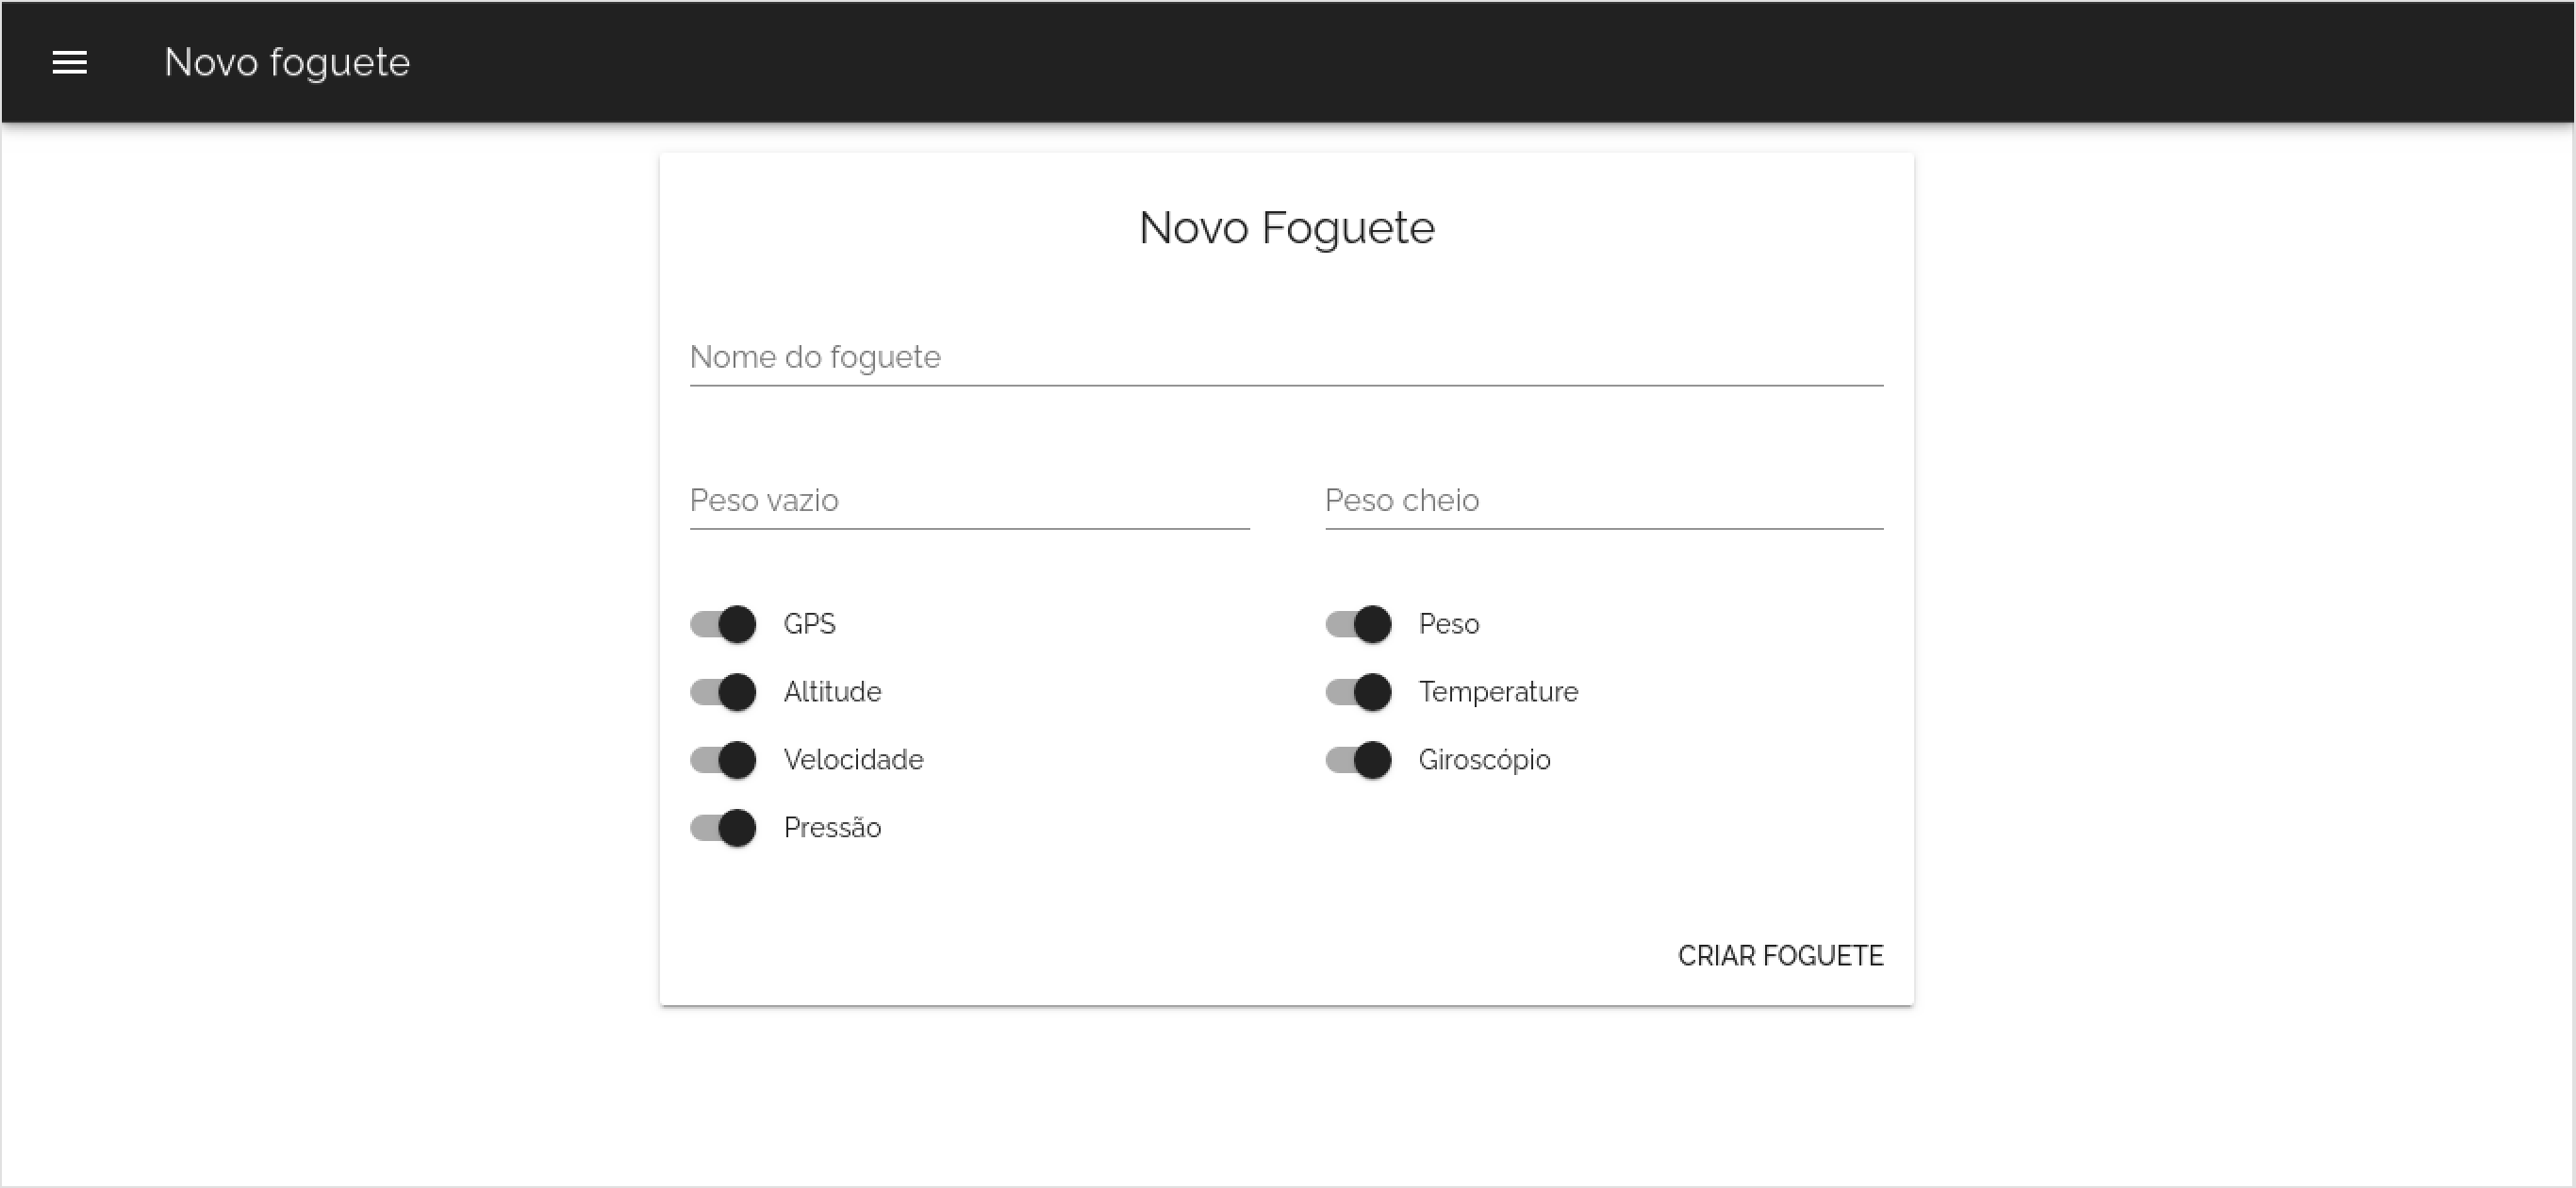
\includegraphics[keepaspectratio=true,scale=0.33]{figuras/telas_software/1.png}
	\caption{Tela de criação de foguetes.}
	\label{fig:cria_foguete}
\end{figure}

Caso o usuário deixe de informar algum dos dados obrigatórios, é feita a validação para informar e impedir que a o foguete seja criado fora dos padrões, como apresentado na Figura \ref{fig:cria_foguete_error}.

\begin{figure}[h!]
	\centering
		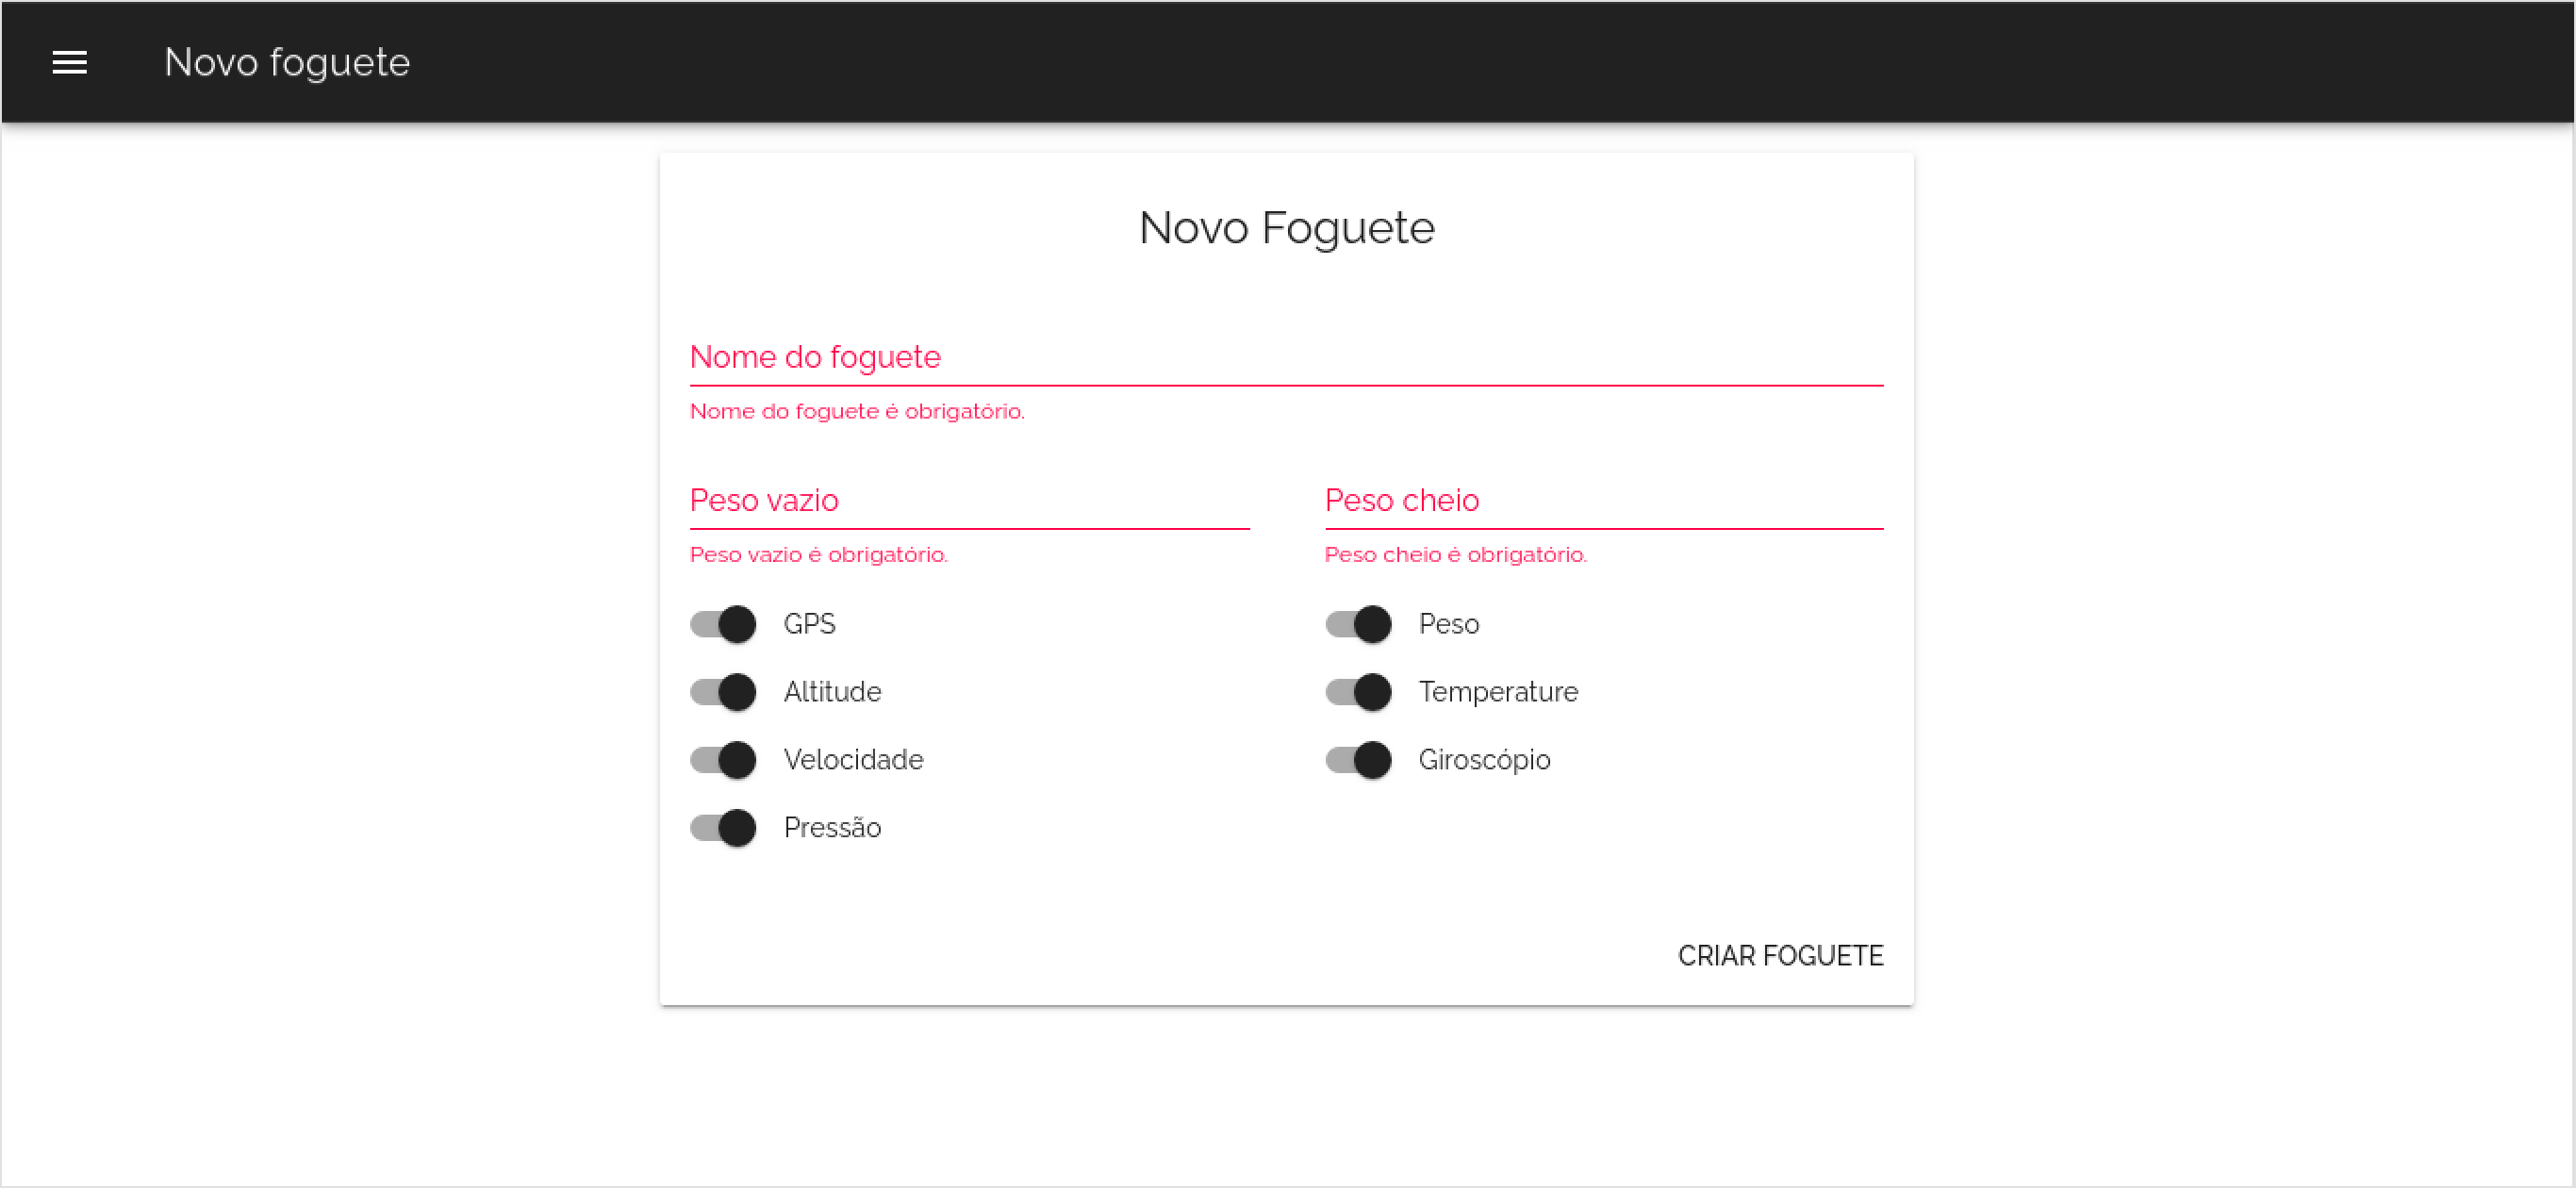
\includegraphics[keepaspectratio=true,scale=0.33]{figuras/telas_software/1-error.png}
	\caption{Tela de criação de foguete com erros demonstrando as validações feitas.}
	\label{fig:cria_foguete_error}
\end{figure}

\subsection{Criação de Hardware e Comandos}

Uma das principais funcionalidade do projeto, é permitir que o software seja utilizado em diferentes hardwares, caso seja compatível com as especificações técnicas. Portanto, a Figura \ref{fig:cria_hardware} permite que os usuários informe qual o nome hardware está sendo usado, o Baudrate e a porta serial para a comunicação.

\begin{figure}[h!]
	\centering
		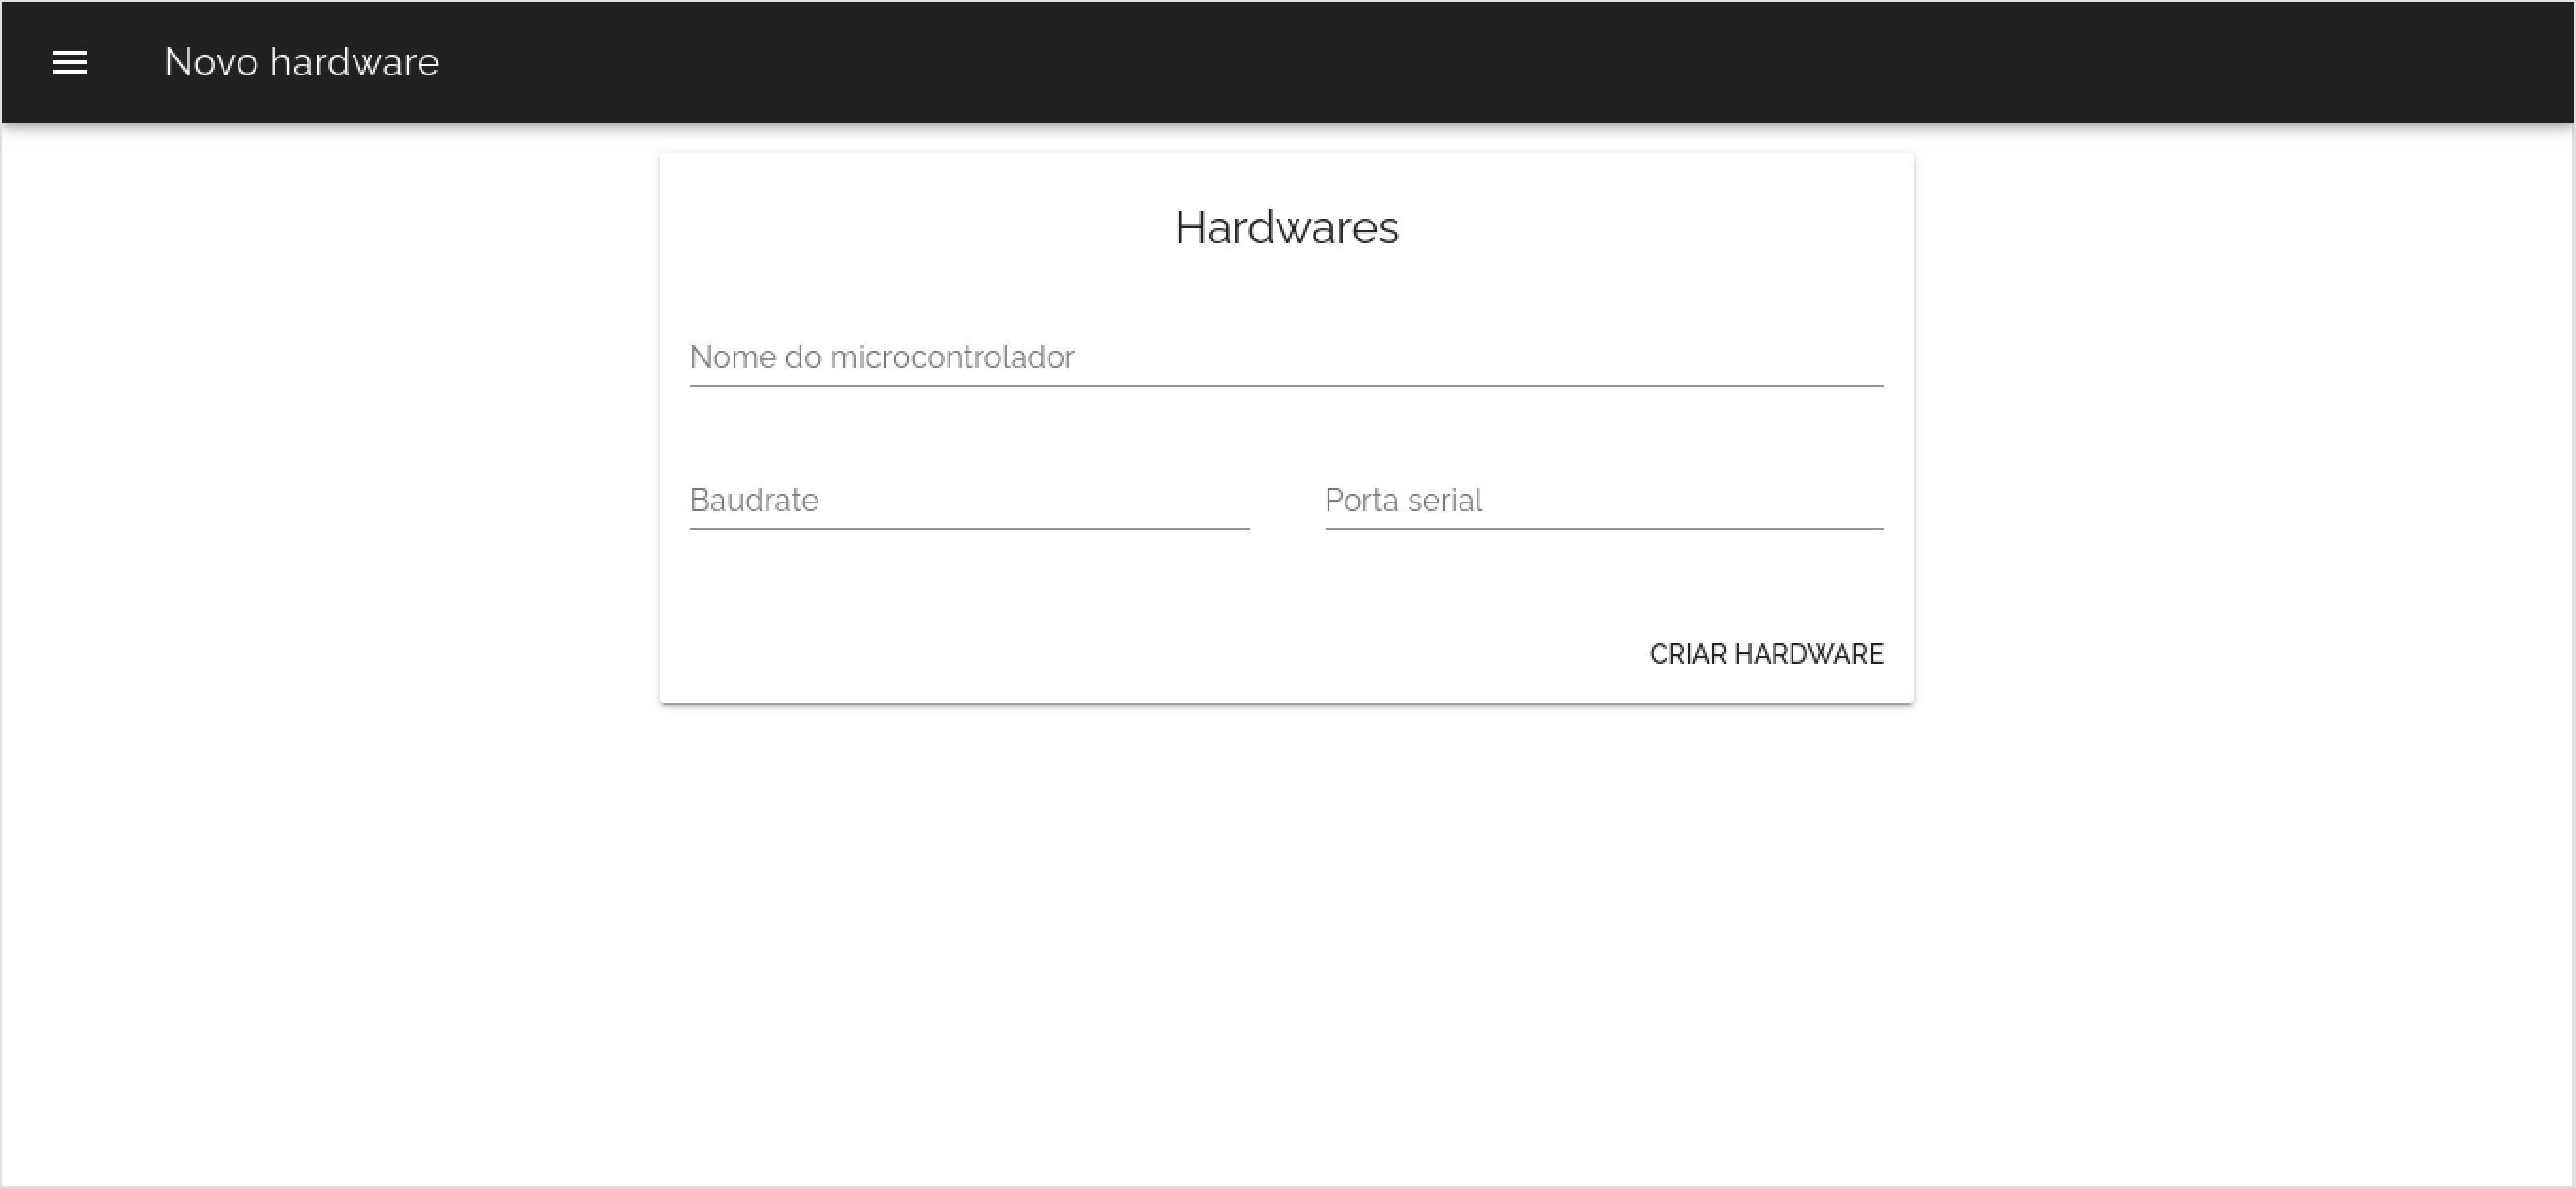
\includegraphics[keepaspectratio=true,scale=0.33]{figuras/telas_software/2.png}
	\caption{Tela de criação de hardware}
	\label{fig:cria_hardware}
\end{figure}

Para garantir o bom funcionamento do sistema, todas essas informações são importantes, portanto foi feito a validação para impedir que o usuário esqueça de inserir alguma informação obrigatória, como apresentado na Figura \ref{fig:cria_hardware_error}.

\begin{figure}[h!]
	\centering
		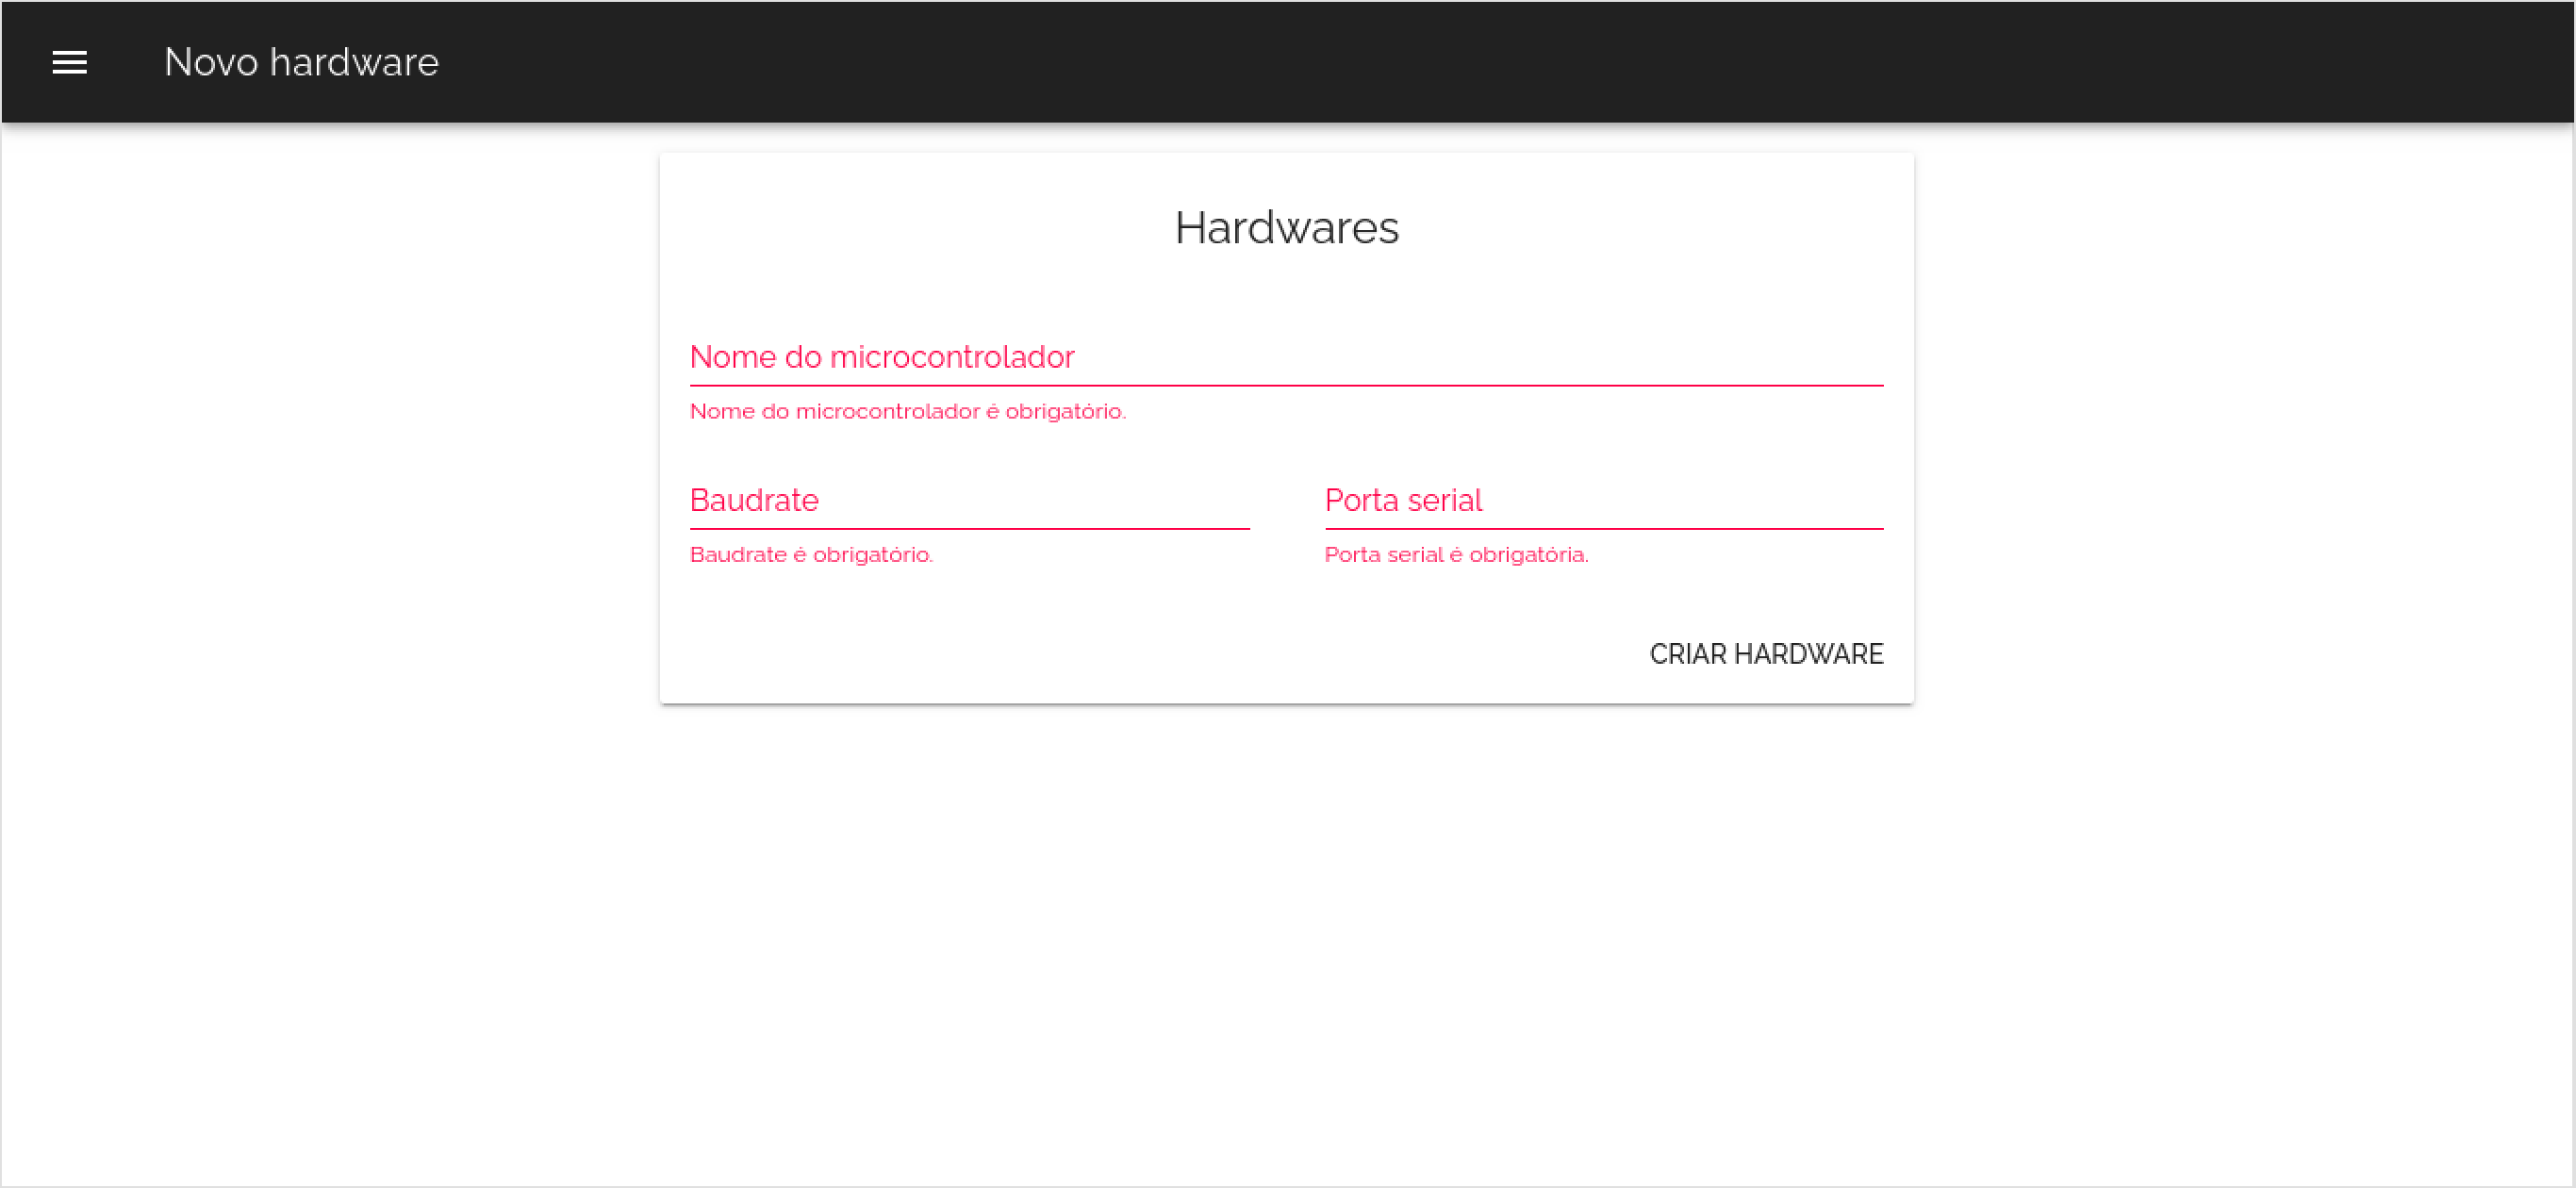
\includegraphics[keepaspectratio=true,scale=0.33]{figuras/telas_software/2-error.png}
	\caption{Tela de criação de hardware com erros demonstrando as validações feitas.}
	\label{fig:cria_hardware_error}
\end{figure}

Ao cadastrar o Hardware a ser usado, é necessário informar também quais comandos esse hardware está apto a receber, como apresentado na Figura \ref{fig:cria_comandos_hardware}. portanto, os usuários e clientes da Capital poderão inserir quais comandos serão enviados ao hardware
\begin{figure}[h!]
	\centering
		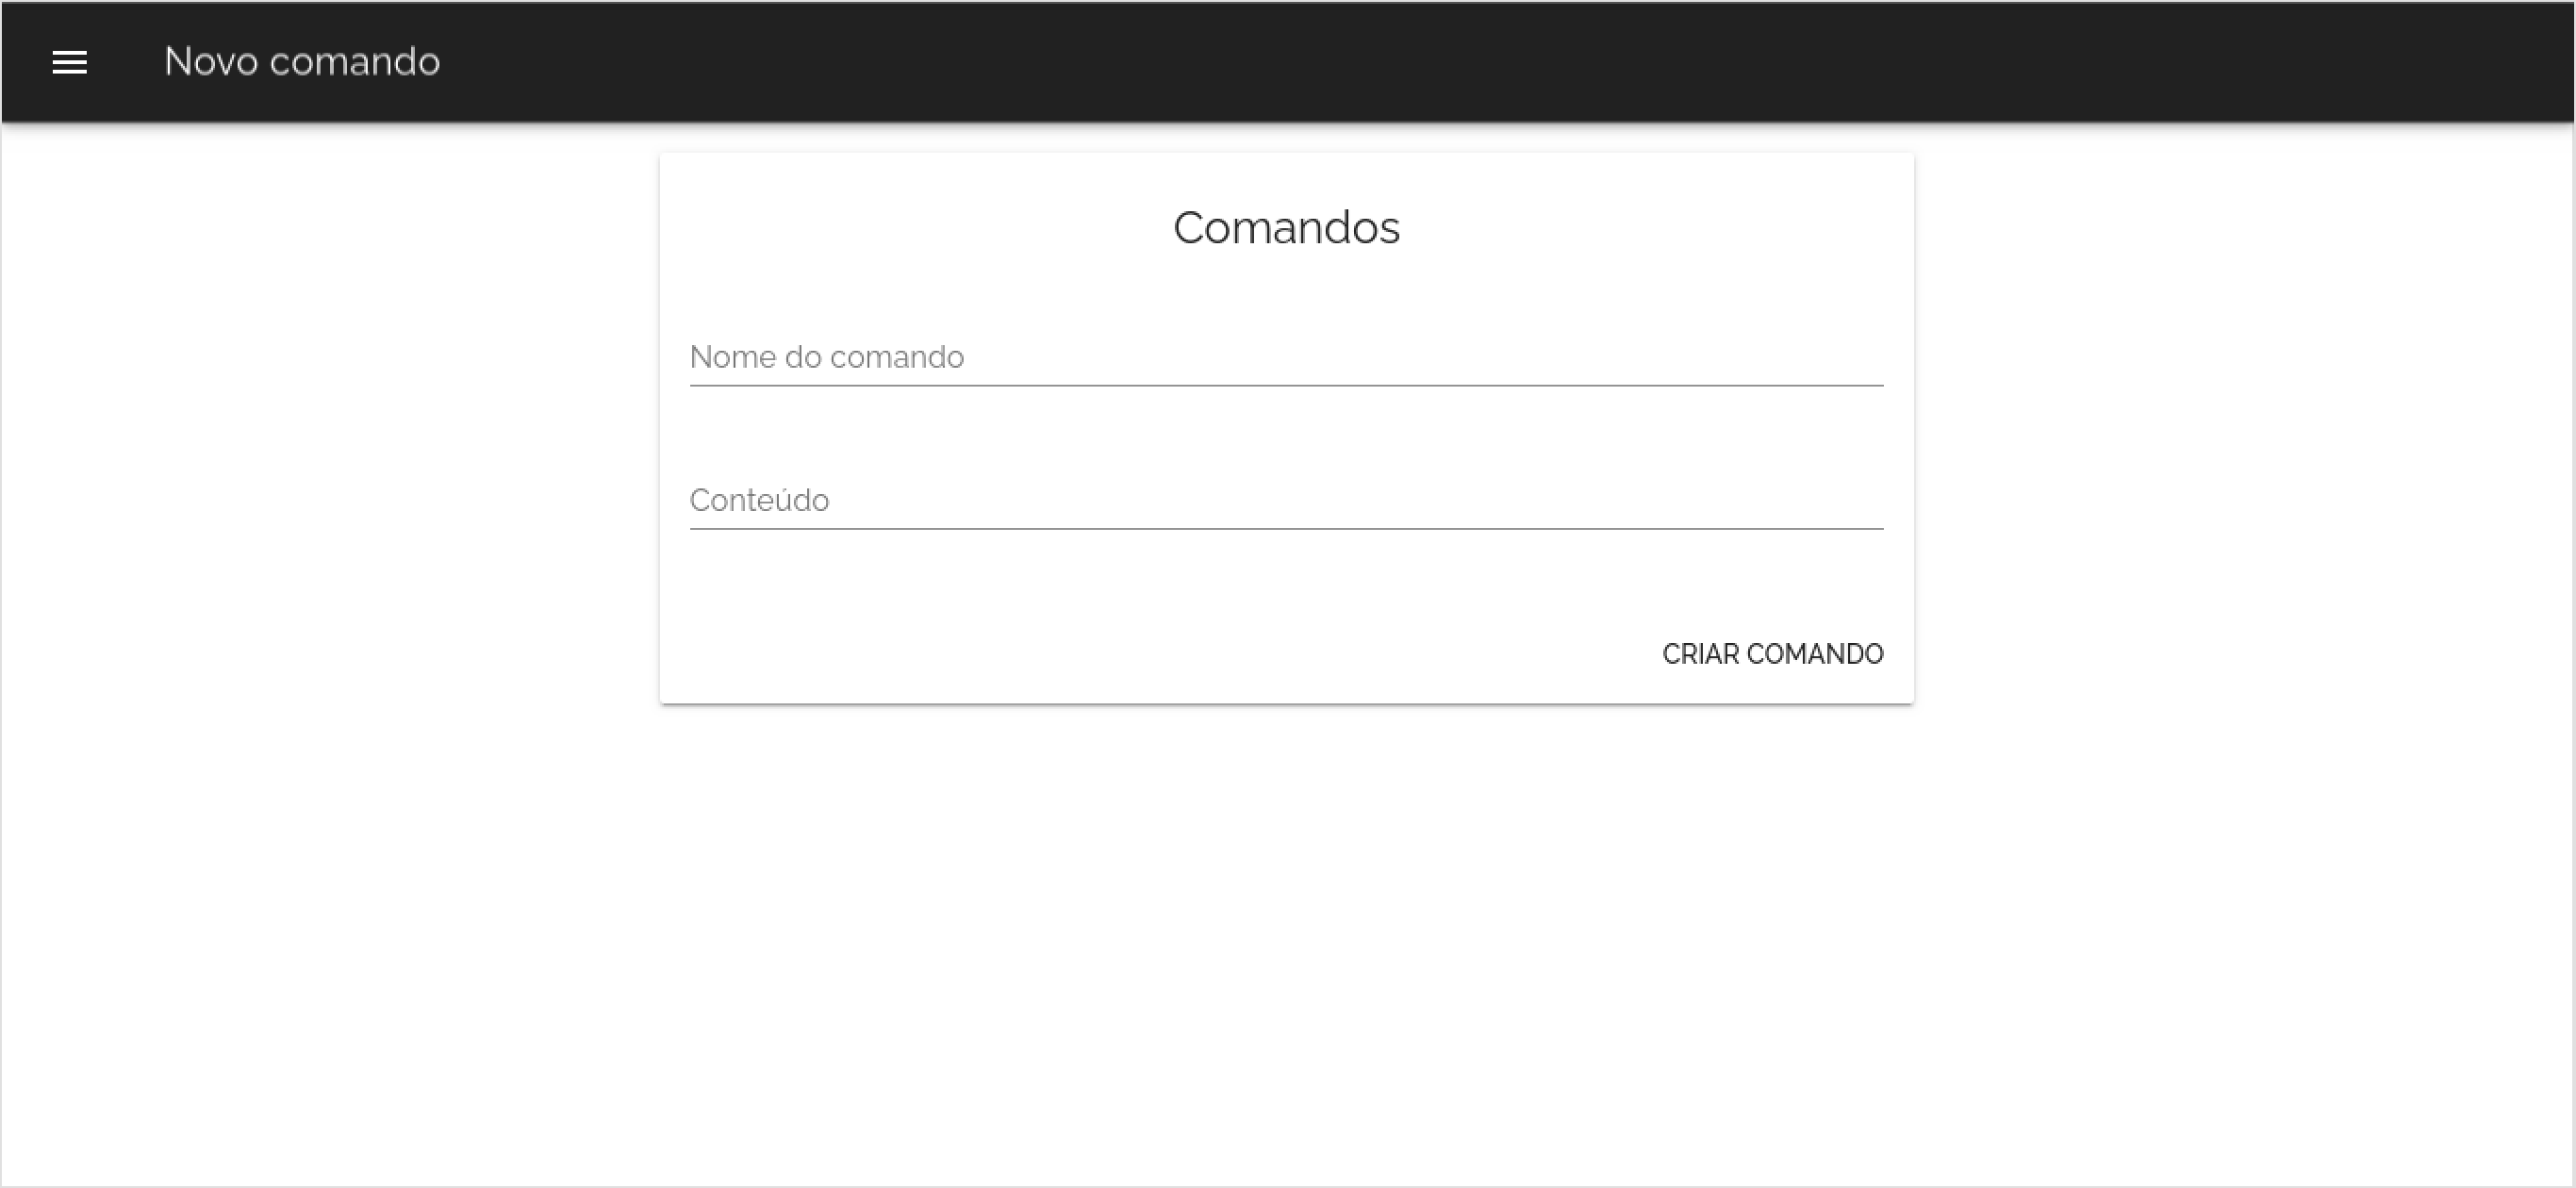
\includegraphics[keepaspectratio=true,scale=0.33]{figuras/telas_software/3.png}
	\caption{Tela de criação de comando para o hardware.}
	\label{fig:cria_comandos_hardware}
\end{figure}

\subsection{Ciclo de missão}

\begin{figure}[h!]
	\centering
		
\includegraphics[keepaspectratio=true,scale=0.33]{figuras/telas_software/4.png}
	\caption{Tela de inicio de missão.}
	\label{fig:inicia_missao}
\end{figure}

Após cadastrar o foguete e o hardware que está sendo usado pode se iniciar o ciclo da missão, iniciando na tela apresentada na Figura \ref{fig:inicia_missao}.

Após confirmar a intenção de iniciar uma missão, é solicitado ao usuário o cadastro da missão informando nome e apogeu esperado (Figura \ref{fig:dados_missao}) e seleciona o foguete como apresentado na Figura \ref{fig:escolhe_foguete}.
\begin{figure}[h!]
	\centering
		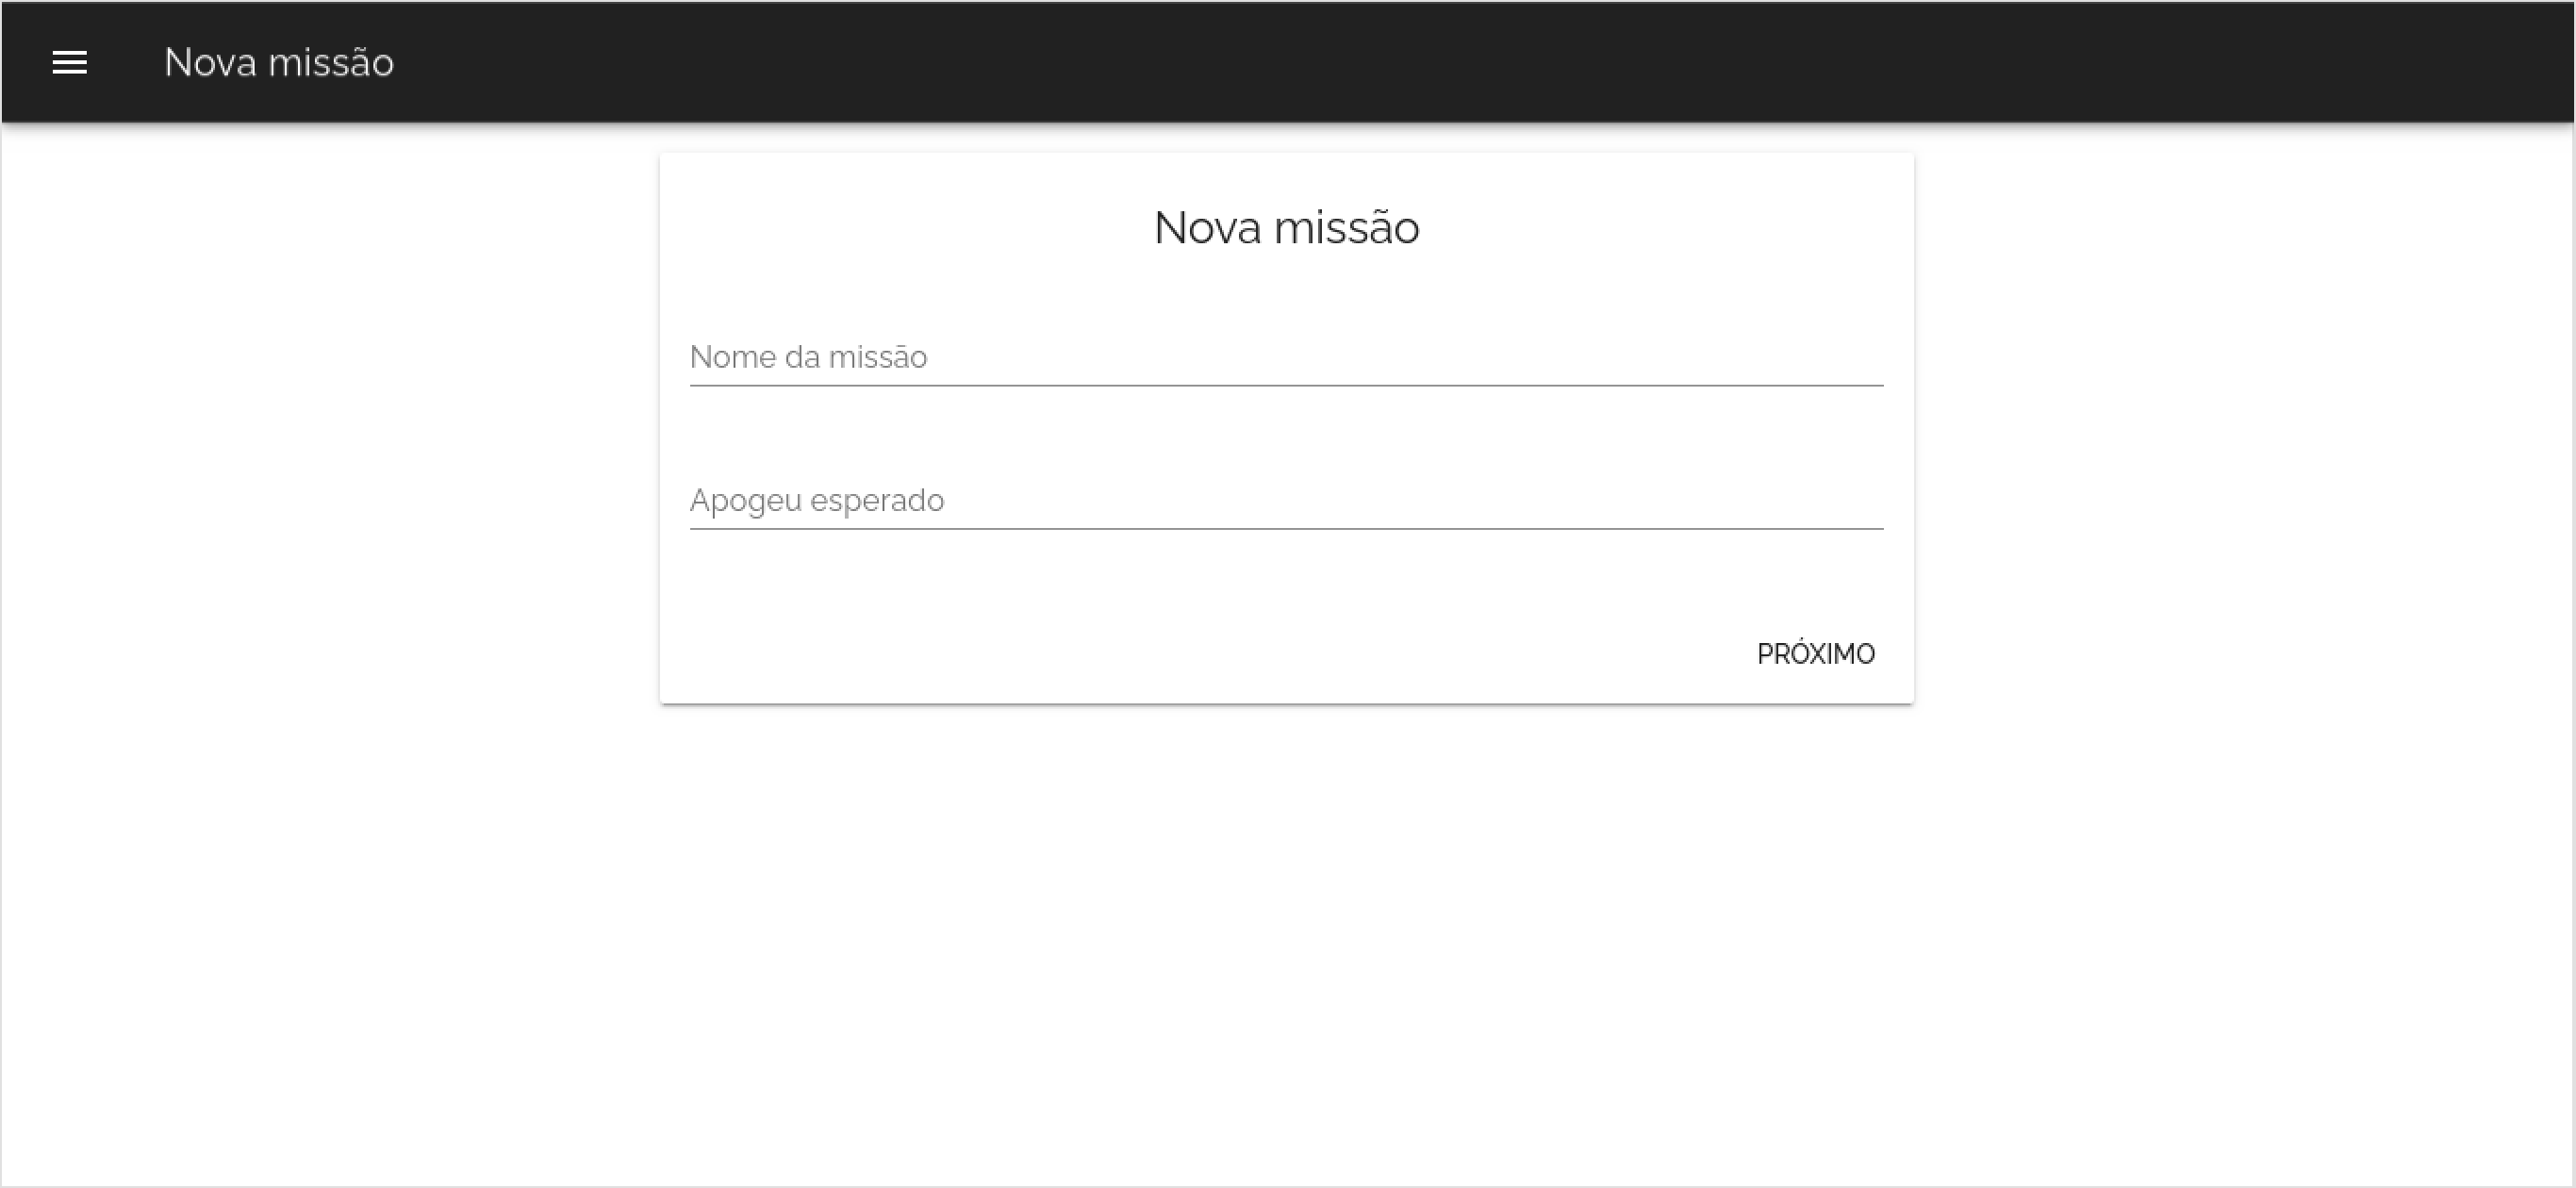
\includegraphics[keepaspectratio=true,scale=0.33]{figuras/telas_software/5.png}
	\caption{Tela para inserção dos dados de uma nova missão.}
	\label{fig:dados_missao}
\end{figure}

\begin{figure}[h!]
	\centering
		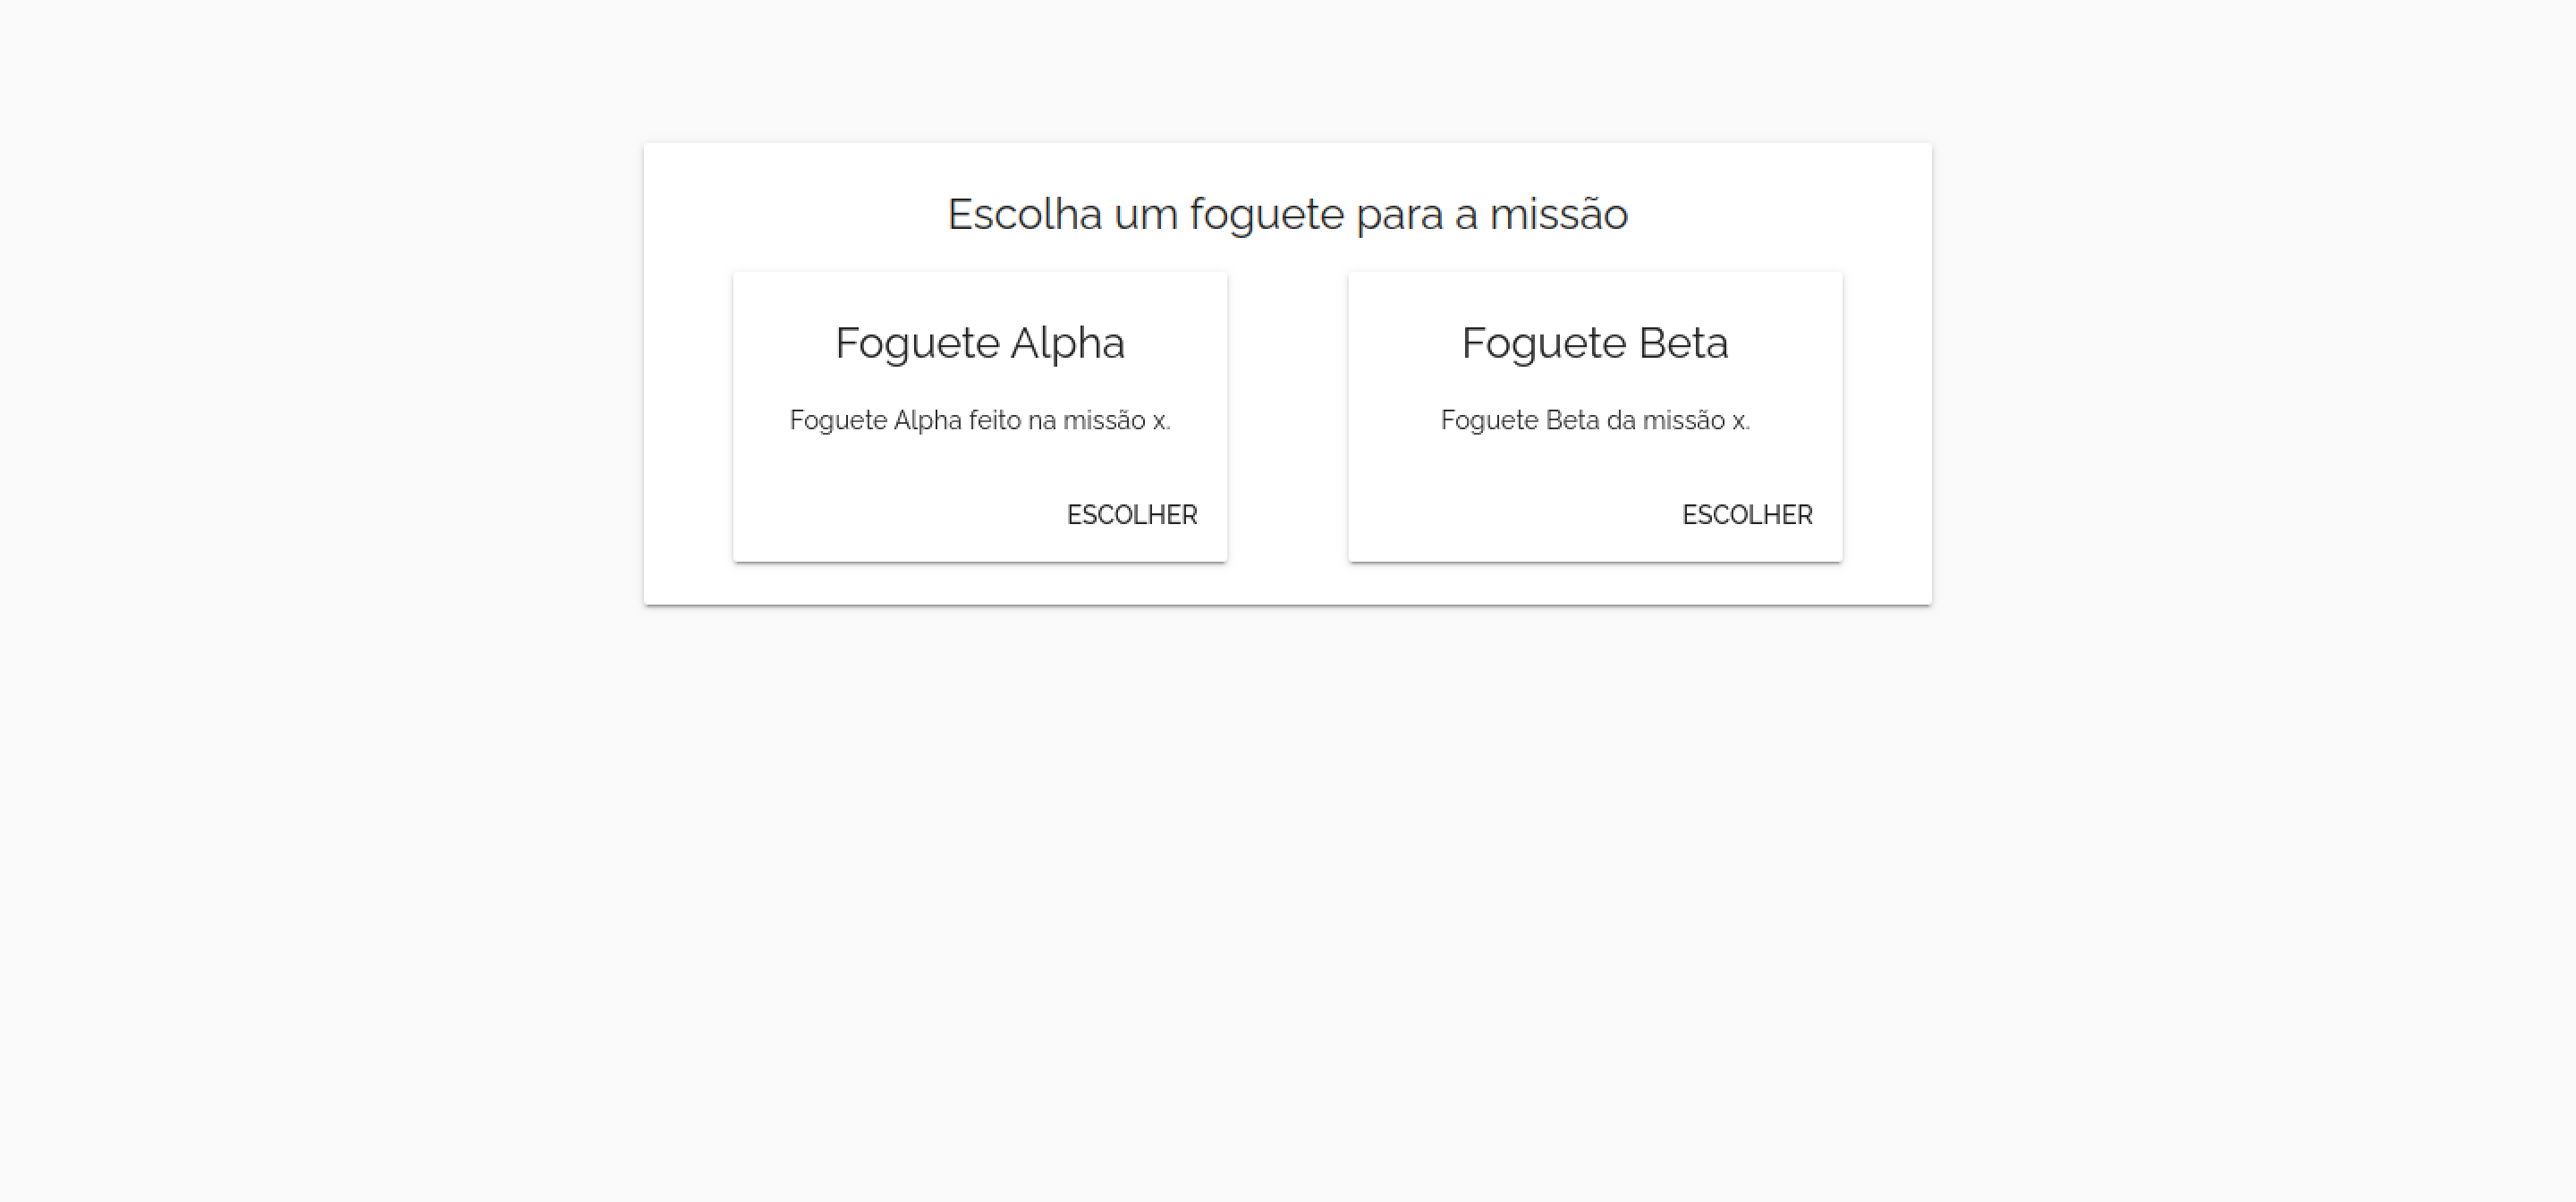
\includegraphics[keepaspectratio=true,scale=0.33]{figuras/telas_software/6.png}
	\caption{Tela de escolha do foguete para a missão.}
	\label{fig:escolhe_foguete}
\end{figure}

Após todo processo de criação de uma missão, o usuário poderá acompanhar o todas as etapas da missão, começando pela etapa de abastecimento, conforme apresentado na Figura \ref{fig:inicio_ignicao}.

\begin{figure}[h!]
	\centering
		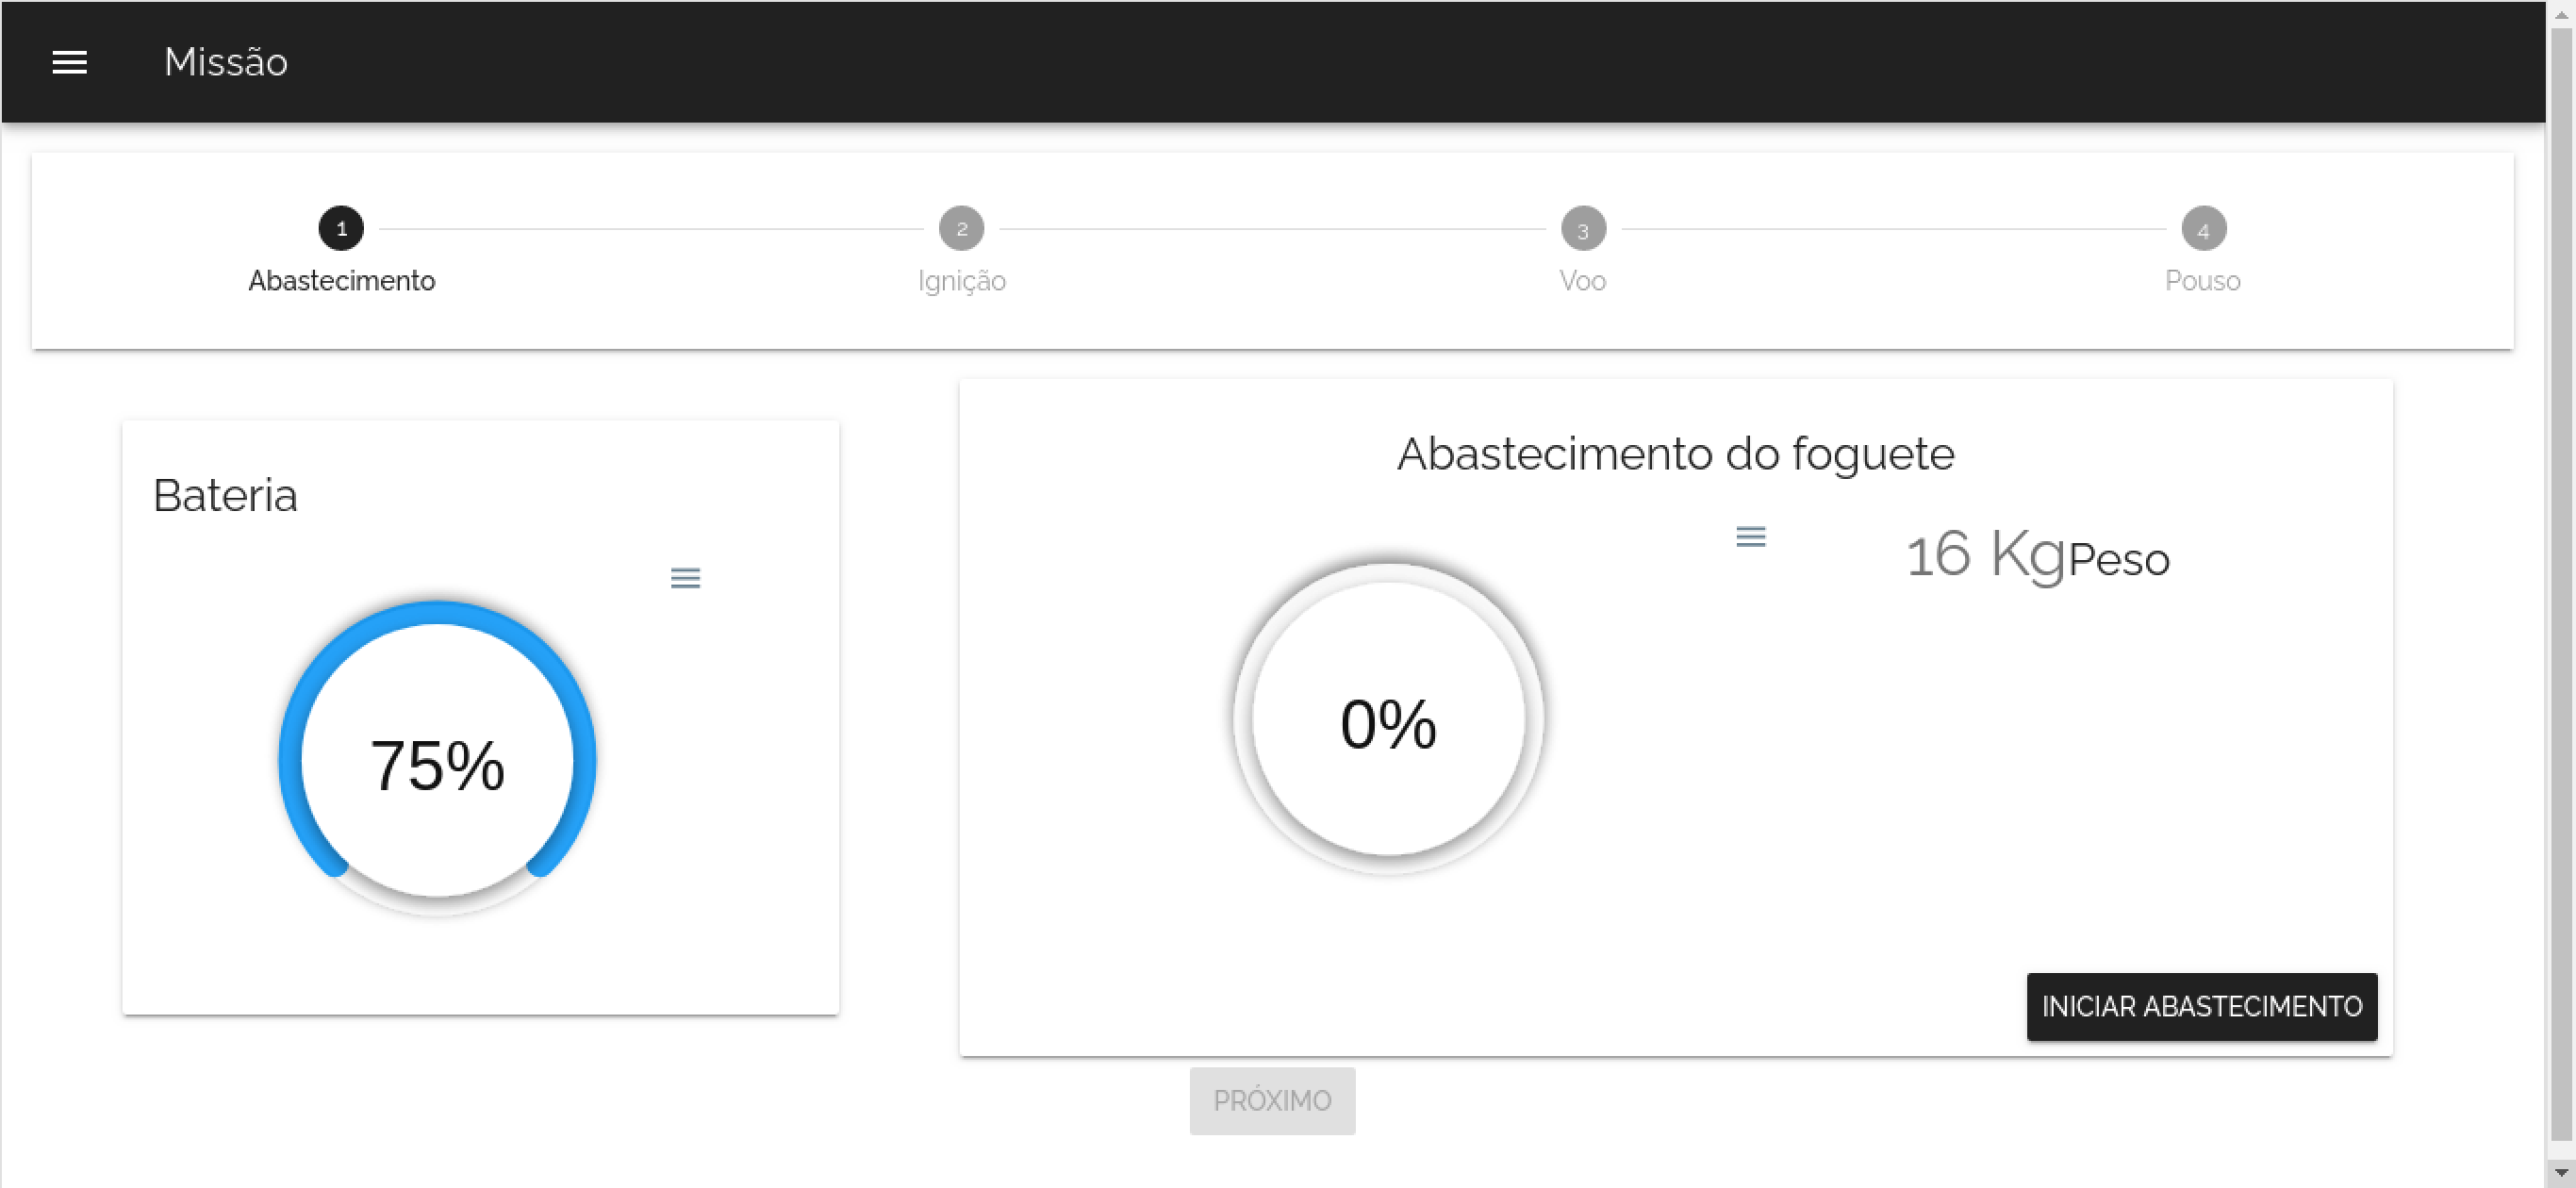
\includegraphics[keepaspectratio=true,scale=0.33]{figuras/telas_software/7.png}
	\caption{Tela inicial da missão, com os dados de abastecimento.}
	\label{fig:inicio_ignicao}
\end{figure}

A Figura \ref{fig:fim_ignicao} mostra o processo de ignição completo, com a porcentagem chegando em 100\%. O botão de "Próximo" é habilitado para o usuário prosseguir para a próxima etapa da missão. Em ambos os gráficos utilizados é possível baixar o gráfico em SVG, PNG ou CSV.

\begin{figure}[h!]
	\centering
		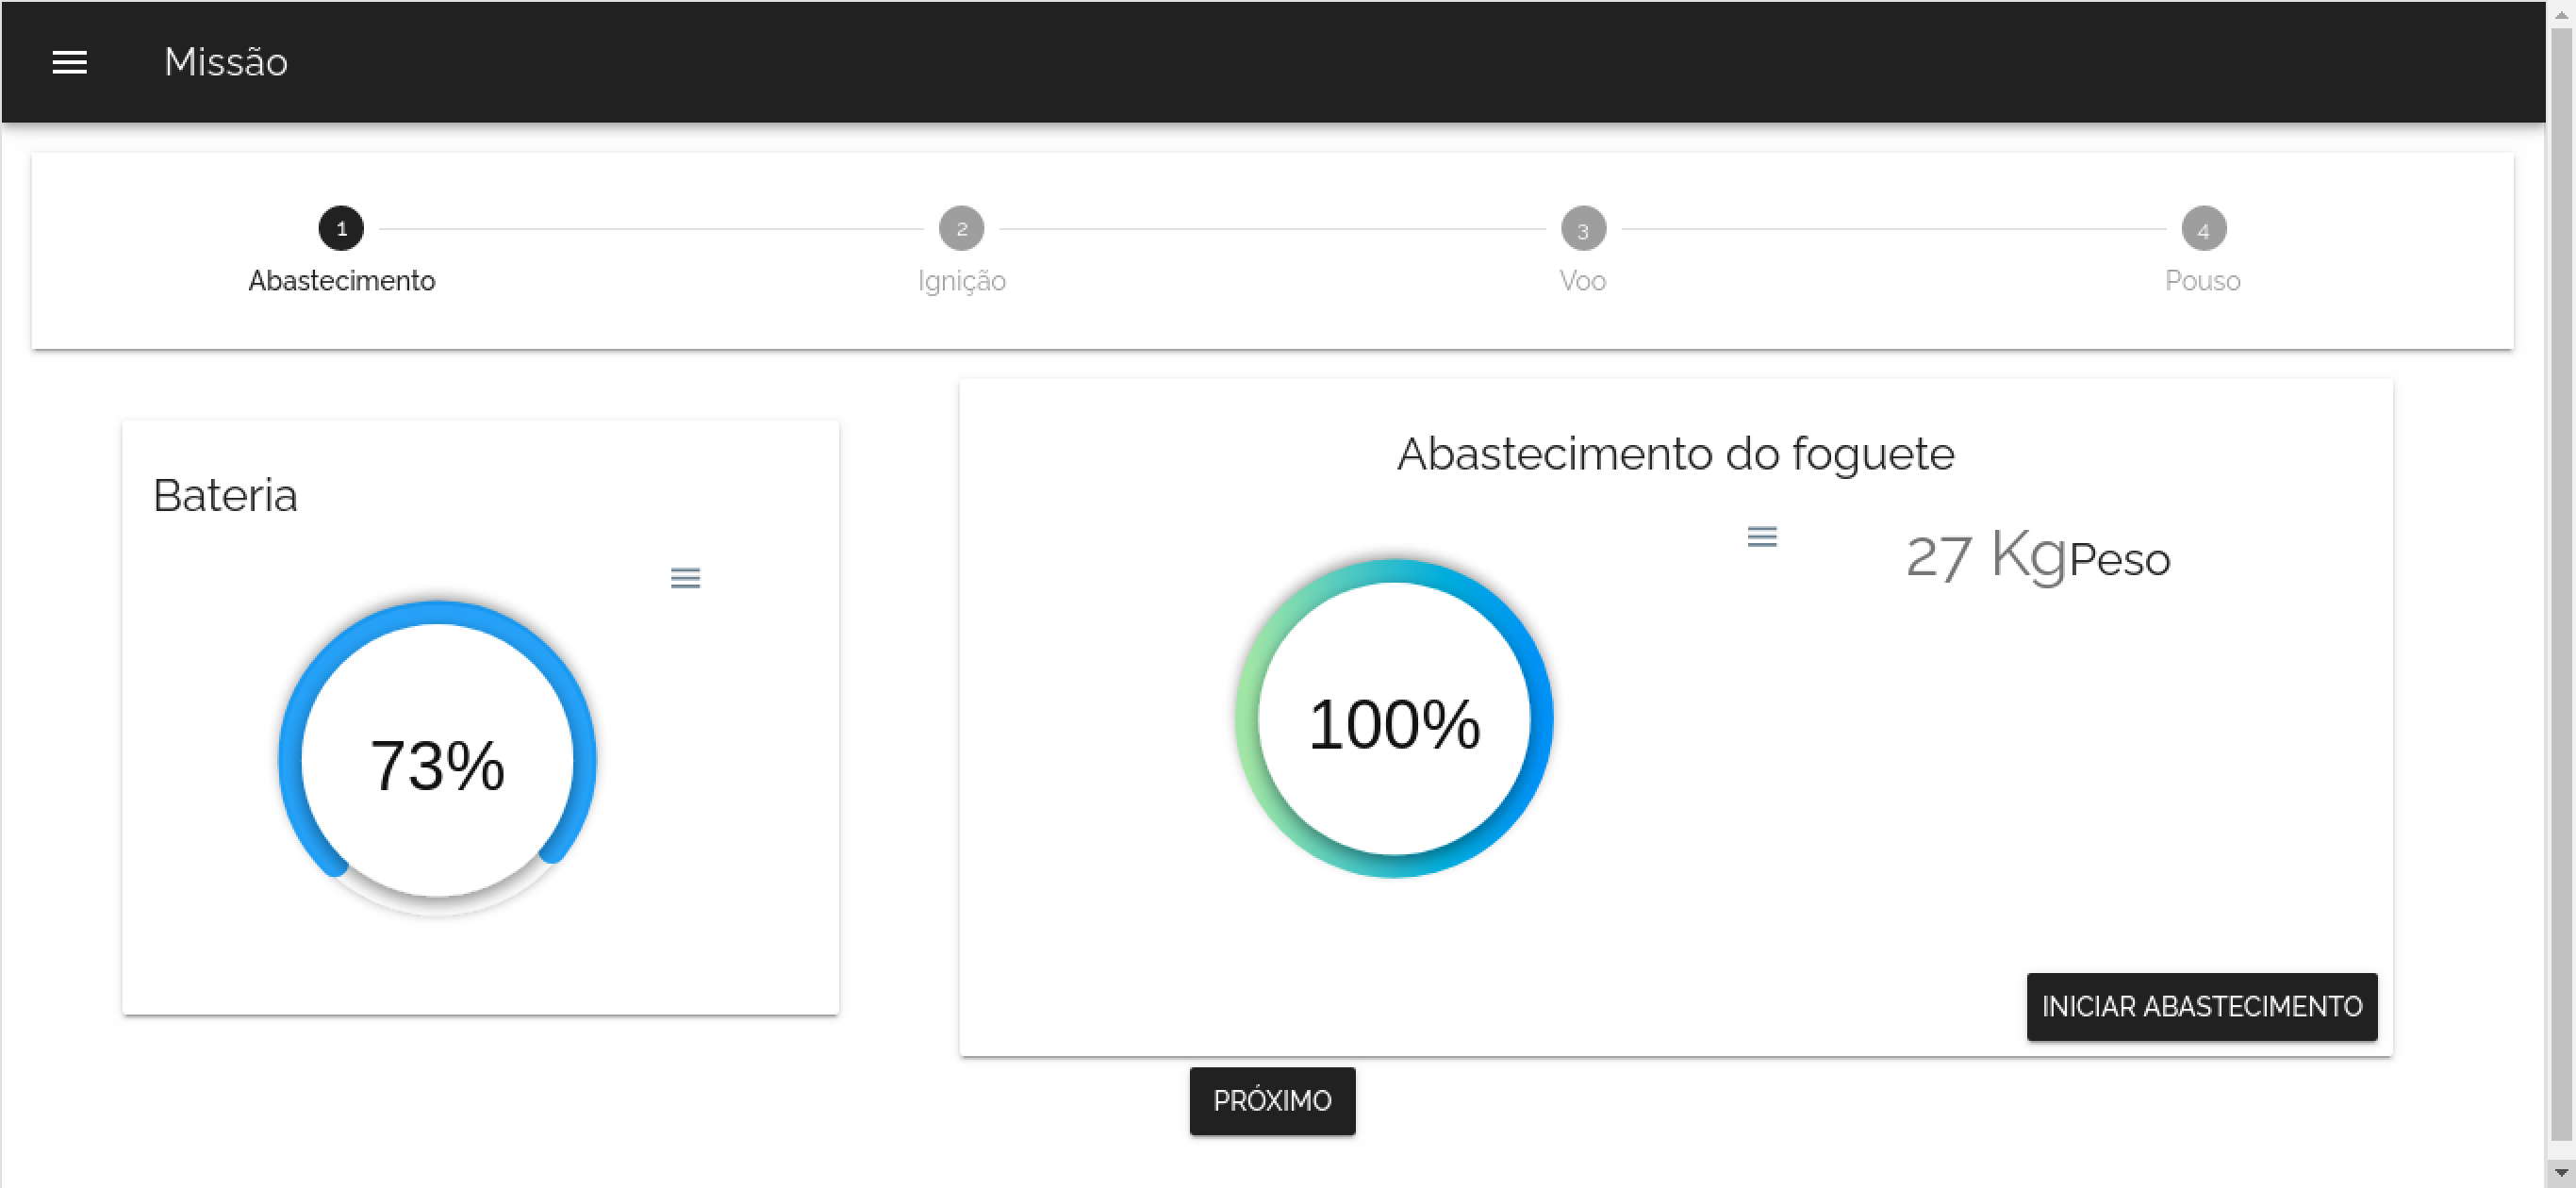
\includegraphics[keepaspectratio=true,scale=0.33]{figuras/telas_software/7-full.png}
	\caption{Tela da fase de abastecimento após o processo concluído.}
	\label{fig:fim_ignicao}
\end{figure}

\section{Construção Backend}

\subsection{API}

A API foi utilizada para desenvolver todos os serviços de consulta e alteração do banco de dados. No Apêndice \ref{documentacao_api} está documentado todos os \textit{endpoints} da API e seus respectivos métodos http. 

\subsection{Serviço de Simulação}

\par Devido a impossibilidade de conectar o software desenvolvido com os componentes de hardware, foi necessário criar um serviço para simular essa comunicação e permitir a verificação e a validação da solução do software, fazendo escritas e leituras em um \textit{Filesystem}. 
\par O \textit{Filesystem} é um arquivo compartilhado para troca de dados. O código de comunicação serial faz a abertura de uma porta de comunicação e lê os dados nesse arquivo  delimitando cada dado por uma vírgula. Os dados recebidos estão dispostos em uma String de 43 caracteres: 

\begin{itemize}
    \item Latitude, 10 caracteres - “Sinal,Centena,Dezena,Unidade,ponto,PrimeiraDecimal,
    SegundaDecimal,TerceiraDecimal,QuartaDecimal,QuintaDecimal”
    \item Longitude, 10 caracteres - “Sinal,Centena,Dezena,Unidade,ponto,PrimeiraDecimal,
    SegundaDecimal,TerceiraDecimal,QuartaDecimal,QuintaDecimal”
   \item Temperatura, 6 caracteres - “Sinal,Dezena,Unidade,ponto,
   PrimeiraDecimal, 
   SegundaDecimal”
   \item Pressão, 9 caracteres - “CentenaMilhar,DezenaMilhar,UnidadeMilhar,Centena,Dezena,
   Unidade,ponto,PrimeiraDecimal,SegundaDecimal”
    \item Altitude, 8 caracteres - “Sinal,UnidadeMilhar,Centena,Dezena,Unidade,ponto,
    PrimeiraDecimal,SegundaDecimal”
\end{itemize}

Essa string está contida num arquivo com extensão .txt ou .csv e o software possui o código necessário para manipular esses tipos de arquivo.

Para simular esse processo foram desenvolvidos algoritmos em \textit{JavaScript} utilizados em rotinas de leitura e escrita de dados e também de emissão dos dados ao \textit{client-side}.

\subsection{Infraestrutura}

A arquitetura computacional da placa Jetson Nano foi desenvolvida em cima da arquitetura computacional Arm-64, e é diferente da arquitetura computacional dos computadores de uso pessoal, que é desenvolvida em cima da arquitetura x86. Por isso, foi necessário o uso de um emulador da arquitetura computacional Arm-64, o QEMU.
O processo de desenvolvimento utilizando o QEMU conta com os seguintes passos:
\begin{itemize}
    \item Instalação do QEMU
    \item Configuração do Docker para utilizar o ambiente de emulação do QEMU
    \item Criação do Dockerfile
    \item Construção da imagem Docker
    \item \textit{Upload} da imagem Docker no DockerHub (docker push)
\end{itemize}

Para a utilização da imagem Docker na placa, o processo é bem simples:
\begin{itemize}
    \item Download da imagem Docker na placa (docker pull)
    \item Execução da imagem (docker run)
\end{itemize}

A Figura \ref{fig:deploy-jetson} mostra graficamente o passo a passo para o deploy da imagem do projeto para a Jetson

\begin{figure}[h!]
	\centering
		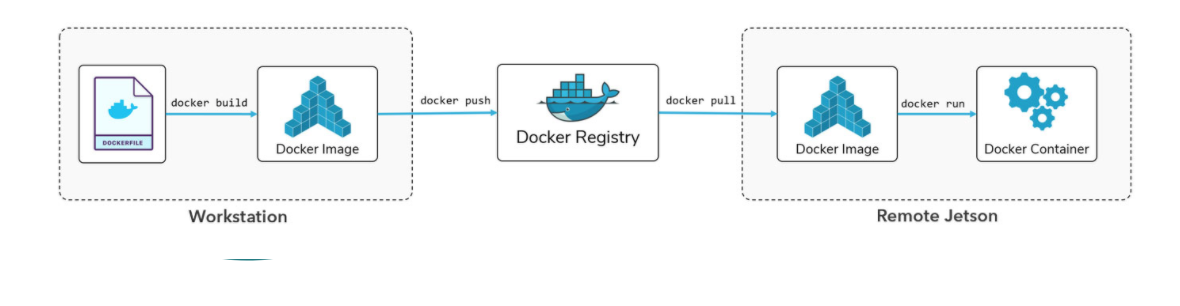
\includegraphics[keepaspectratio=true,scale=0.33]{figuras/deploy-quemu.png}
	\caption{Deploy de uma imagem docker na Jetson \cite{Deploy-Jetson} }
	\label{fig:deploy-jetson}
\end{figure}

Mais informações sobre esse processo podem ser verificados no link a seguir: \href{https://www.stereolabs.com/docs/docker/building-arm-container-on-x86/}{Arm container on x86}.


\chapter{Eletrônica}
\par A solução de eletrônica do projeto consiste em garantir todo o funcionamento eletrônico do projeto, que foi dividido em três subáreas: telemetria, sensoriamento e controle do abastecimento/ignição do foguete.
\par Como o principal objetivo do projeto é construir um sistema de controle e monitoramento do foguete que permita  ser feito a uma distância segura. Para isso, foi pensada uma solução envolvendo telemetria tanto para colher os dados quanto para enviar sinais de comando.Para melhor detalhamento da solução, foi construído um  \href{https://drive.google.com/file/d/12-pXv5L2Z5AuyWWVIr8VZ4WMghu7SYDw/view?usp=sharing}{Diagrama Geral}  para melhor detalhamento do projeto na parte de \textit{hardware}, a figura \ref{fig:Diagrama de Blocos} no apêndice \ref{Diagrama de blocos do sistema} resume bem a solução proposta.
 
\section{Telemetria}

\par É um processo remoto de aquisição ou envio de dados, ou seja, é utilizado para medir, rastrear ou até mesmo controlar à distancia alguma coisa. Esse processo é feito geralmente por um sistema de comunicação sem fio, como por exemplo por radiofrequência ou via satélite. \cite{Telemetria_AERONALTICA}.
\par Atualmente,  a telemetria está presente em diversos ramos da vida cotidiana do ser humano: na apuração das informações de um automóvel, no controle meteorológico, na agricultura e em outras diversas atividades.Para o projeto proposto, entende-se que o uso da telemetria em tempo real é extremamente vantajoso para a aquisição de dados durante o voo do foguete e para o controle autônomo do seu abastecimento/ignição.
\par Como requisito de segurança, é necessário fazer o controle  do foguete à distância. O recomendado pelas regras da LASC, competição a qual o cliente pretende participar, é uma distância mínima de 500m (lembrando que o foguete pode atingir uma altura de voo de aproximadamente 1km). Ou seja, fazer a aquisição de dados e o controle de abastecimento e ignição via cabo seria muito dispendioso, ou mesmo inviável, sujeito a maiores riscos de falhas, ou ficando na dependência de coletar os dados armazenados na memória do foguete somente após sua recuperação. Por essas razões, entende-se que é necessário realizar a telemetria em tempo real. Para melhor entendimento, na figura \ref{fig:Diagrama lançamento}   encontra-se o esquemático de um lançamento de foguete.

\begin{figure}[!htb]
\centering
\includegraphics[scale=0.5]{figuras/LANÇAMENTO.png}
\caption{Diagrama do Lançamento.}
{\footnotesize Fonte: Elaborado pelo autor.}
\label{fig:Diagrama lançamento}
\end{figure}

\par Como trata-se de uma função específica, o controle à distância e a aquisição de dados do pré-lançamento, do lançamento, do apogeu até a chegada do foguete no chão, é necessário compreender o problema e levantar requisitos para escolher a melhor forma de fazer a telemetria do projeto.
\par Foram analisadas diversas formas de fazer a telemetria, entre elas estão: a telemetria feita por radiofrequência, Lora, Wi-Fi, ZigBee, GPRS, Bluetooth, entre outras, analisando os seguintes requisitos: 
\begin{itemize}

\item Alcance;
\item Taxa de Transição de dados;
\item Protocolo de Comunicação;
\item Frequência dos Protocolos;
\item Potência de Transmissão; 
\item Interface de Dados;
\item Consumo.

\end{itemize}

\par Por fim, analisando diversos componentes, foi definido que a Placa Lora Esp32 da HELTEC, figura \ref{fig:Placa Esp32 Lora }, atende os requisitos do projeto citados acima, garantindo assim o funcionamento de qualidade do projeto, sendo que o principal motivo foi a distância alcançada pelo transmissor e a baixa perda de potência em sua transmissão.

\begin{figure}[!htb]
\centering
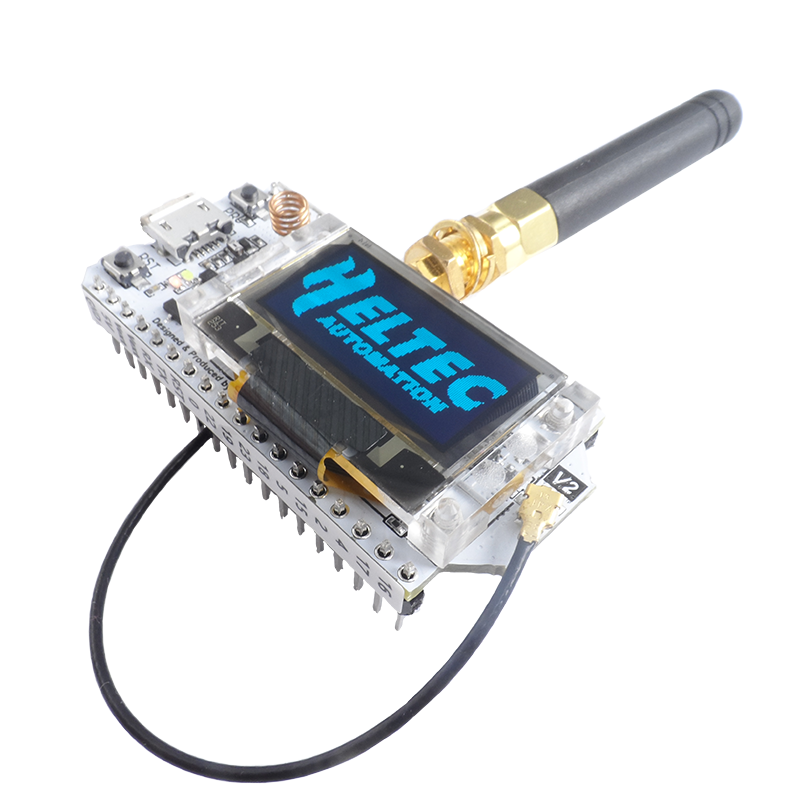
\includegraphics[scale=0.35]{figuras/SAM_0748_800X800.png}  
\caption{Placa Lora Esp32 da HELTEC.}
{\footnotesize Fonte:\cite{datasheet_ESP32}}
\label{fig:Placa Esp32 Lora }
\end{figure}
\par Contudo, como forma de garantir a integridade dos dados do lançamento, os mesmos também serão gravados num MicroSD dentro do foguete, evitando assim, a perda de dados por uma eventual falha na telemetria. 

\subsection{Lora}

\par A comunicação feita via Lora (Long Range) é um método de comunicação à distância sem fio, utilizando radiofrequência, pode ser considerado um marco para o IOT - internet das coisas, possibilitando a realização de diversos projetos com sua utilização.
\par A técnica de modulação utilizado pela LoRa é baseada na modulação \textit{Chirp Spread Spectrum} (CSS), que é bastante semelhante à modulação FSK (\textit{Frequency-shift keying}), onde a frequência varia linearmente ao longo do tempo. Contudo, o LoRa tem um ganho de potência maior em relação a modulação FSK, possibilitando assim maior alcance dos sinais.
\par A tecnologia LoRa possui uma uma estrutura de pacote de dados que pode variar entre 2 até 255 bytes, dependendo das configurações a serem utilizadas, além de ser possível alcançar uma taxa de transmissão de até 50 Kbps. Para isso, é necessário  utilizar artifícios e técnicas de canais \cite{transmissaoLoRa}. A LoRa pode ser utilizada em diversas bandas ISM (Industrial Sientific and Medical), que regula as frequências para livre desenvolvimento industrial, sendo que cada país tem seu órgão responsável para distinguir qual faixa pode ser utilizada, no Brasil se trata da ANATEL - Agência Nacional de Telecomunicações. Segundo a Resolução n$^{\circ}$ 726, de 05 de maio de 2020, que regulamenta as faixas livres de frequência no Brasil\cite{resolucao726}, a LoRa enquadra-se na faixa de frequência livre no Brasil, que varia de 902 a 928 MHz, entre outras, portanto o transmissor LoRa opera em 915MHz no continente americano se enquadrando na resolução supracitada, figura \ref{fig:Faixa de Frequência ISM}.

\begin{figure}[!htb]
\centering
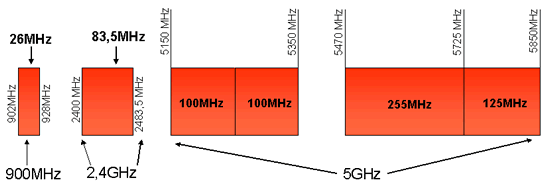
\includegraphics[width=\textwidth]{figuras/faixas de frequencia .png}  
\caption{Faixa de Frequência ISM no Brasil.}
{\footnotesize Fonte:\cite{faixafreq}}
\label{fig:Faixa de Frequência ISM} %\url{https://www.teleco.com.br/} }
\end{figure}
\par A modulação LoRa codifica a mensagem em pulsos de \textit{chirps}, sendo que possui alguns parâmetros importantes para o melhor entendimento do funcionamento do mesmo: a largura de banda, a frequência da portadora e a taxa de código\cite{desepenhoLoRa}.

\par A frequência da portadora é definida como a frequência central da informação, que é especificada pela região utilizada pelo equipamento (como citado anteriormente, a frequência é de 915MHz para o continente americano).

\par A largura de banda (\textit{Bandwidth} - BW) define o tamanho da faixa de frequência que a mensagem vai ser transmitida, ou seja a quantidade de informação que irá caber na mensagem. No protocolo de comunicação LoRa, há 3 configurações possíveis programáveis:  125KHz, 250KHz e 500KHz. Já o fator de espalhamento (\textit{Spreading Factor} - SF) determina a variação da duração do pulso \textit{chirps}, figura \ref{fig:sflora},sendo um parâmetro da modulação LoRa que tem como objetivo reduzir perdas na transmissão, porem há uma perda na taxa de transmissão. O SF pode variar de 7 até 12, ou seja, quanto maior o SF, maior será o tempo da mensagem no ar e, consequentemente, menor o tamanho da mensagem enviada. Na figura \ref{fig:sfloraDISTANCIA}, pode-se notar a representação dessa variante.

\begin{figure}[H]
  \centering
  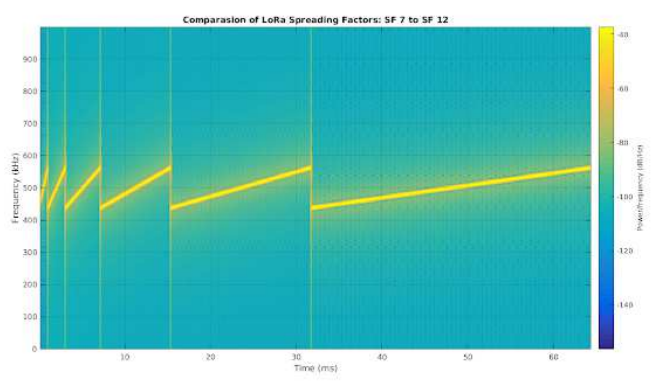
\includegraphics[scale=0.75]{figuras/sflora.png}
  \caption{Diferentes símbolos para SF diferentes em LoRa. }
 { \footnotesize Fonte:\cite{lorasf1}} 
  \label{fig:sflora}
\end{figure}

\begin{figure}[H]
  \centering
  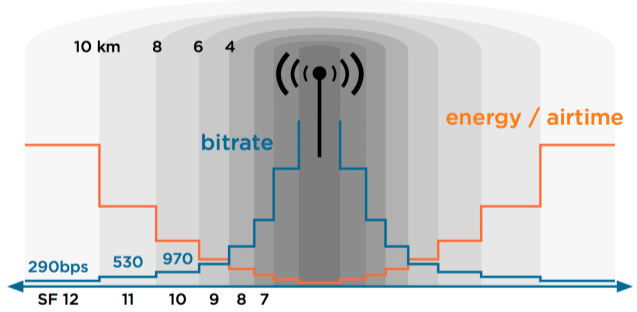
\includegraphics[width=\textwidth]{figuras/SFdistanci.png}
  \caption{Diferentes distancias para SF diferentes em LoRa. }
 { \footnotesize Fonte:\cite{lorasf}} 
  \label{fig:sfloraDISTANCIA}
\end{figure}

\par A taxa de código (\textit{Code Rate} - CR), é o modelo utilizado pela modulação LoRa para correção de erros na transmissão, é baseado em uma técnica correção posterior de erro, (\textit{Forward Error Corrector} - FEC). Portanto, o CR define a quantidade de bits de redundância serão utilizados na correção dos erros,  recuperando a mensagem, por sua vez, é dado pela equação \ref{cr} \cite{aplicacaolora}.

\begin{center}
\begin{equation}
\label{cr}
    CR=\frac{4}{4+n},\ com\  n \in \left\{1,2,3,4\right\}
\end{equation}
\end{center}

\par Por exemplo, usando n=1, temos um CR= $ \frac{4}{5}$, ou seja, $ \frac{1}{5}$ do pacote será composto por bits de redundância e os outros $ \frac{4}{5}$ serão compostos pela mensagem propriamente dita.

\par A taxa de bits (\textit{Bit Rate} - Rb) é a quantidade de bits que podem ser transmitidos por segundo em um determinado meio. Na modulação LoRa pode ser calculada pela equação \ref{taxa de bits }. Na figura \ref{fig:taxalora}, pode-se observar a variação da taxa de transmissão LoRa variando os parâmetros SF e a BW. 


%decidimos usar um SF entre 7 e 8, que atende nossa distancia pretendida com uma largura de banda de 500KHz e uma taxa de código de $ \frac{4}{5}$ ou$ \frac{4}{6}$que garante uma quantidade grande de dados a serem transmitidos.  

\begin{center}
\begin{equation}
 \label{taxa de bits }
 Rb =SF  \times \frac{BW \times CR } {2^{SF}}  ,\ com\  SF \in \left\{7,8,9,10,11,12\right\}
 \end{equation}

 \end{center}
Onde:

\begin{itemize}

\item Rb =Taxa de bits/s,
\item BW=Largura de banda(Hz),
\item SF=Fator de espalhamento,
\item CR=Taxa de código.

\end{itemize}

\begin{figure}[H]
  \centering
  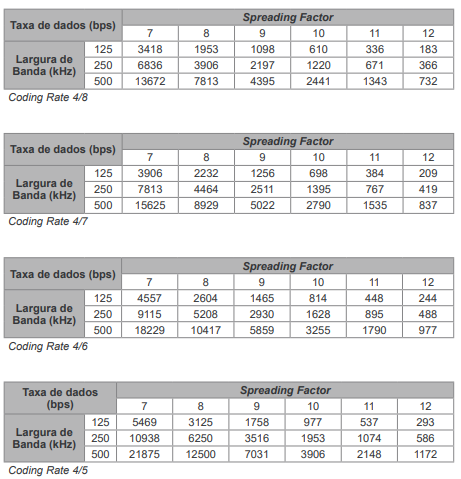
\includegraphics[width=\textwidth]{figuras/tabela de taxa lora.png}
  \caption{Diferentes taxa para SF e BW diferentes em LoRa. }
 { \footnotesize Fonte:\cite{aplicacaoloratabela}} 
  \label{fig:taxalora}
\end{figure}

\par Para configurações dos módulos SX1276 LoRa nas ESP 32 que compreende o trabalho em questão, foi feito levantamento dos dados a serem transmitidos e seu formato. A "Semtech" padronizou um formato especifico da mensagem para facilitar a conexões entres os transmissores e receptores sendo composta por (identificação + \textit{playload}), ou seja a identificação é o preâmbulo que é responsável pela si cronização entres o transmissor e receptor e o cabeçalho que é opcional que leva a informação do tamanho da mensagem e o \textit{playload} que é propriamente dito a mensagem mais os bits de redundância\cite{loras}.      
\par Ficou definido uma ordem fixa de agrupamento dos dados, assim, montando um pacote, além do mais que os dados seriam salvos  no formato em que os valores fossem separados por vírgulas (\textit{Comma Separated Values} - .CSV) que permite sua utilização de maneira mais prática tanto para seu armazenamento em banco de dados quanto para a criação de gráficos pertinente aos dados enviados.
\par Obtendo o tamanho de cada pacote, foi  analisado qual seria o pior caso para a transmissão, que no caso  é o pacote  de transmissão dos sensores de dentro do foguete para a RGS, este possui a string:\\
{ \footnotesize “InMSG, LATITUDE,LONGITUDE,TEMPERATURA,PRESSÃO,ALTITUDE,VELOCIDADE,Fimmsg”.}
\par A maior \textit{string} é constituída de 50 caracteres mais 6 vírgulas para separação dos dados, totalizando 56 caracteres, e sendo o maior pacote de dados que necessitará ser enviado. Dado que cada caractere possui 8 bits de acordo com o padrão da norma ISO/IEC 8859-16:2001, pode-se calcular o número de bits da maior \textit{string} a ser transmitida que contém aproximadamente 450 bits.

\par O cálculo das  para da taxa de transmissão é representado pela equação \ref{taxa de bits }, entretanto  \textit{Semtech} disponibiliza uma calculadora para levantamento dos dados da transmissão e recepção como apresentado nas figuras \ref{fig:calculo LoRa1}, \ref{fig:calculo LoRa2} em que foi definido os seguintes parâmetros dados as especificações do projeto, SF=8, BW=125 KHz, CR=$ \frac{4}{5}$,ou seja, um \textit{playload} de 68 bytes é necessário por estar-se usando o CR supracitado que acresce em $\frac{1}{5}$ o numero total de bits, sendo estes de redundância. Assim dado a frequência da portadora de 915 MHz e potência de transmissão de 20 dBm   obten-se uma taxa de transmissão de aproximadamente de 2000 bps suprindo com uma margem considerável  a demanda do projeto. 


\begin{figure}[H]
  \centering
  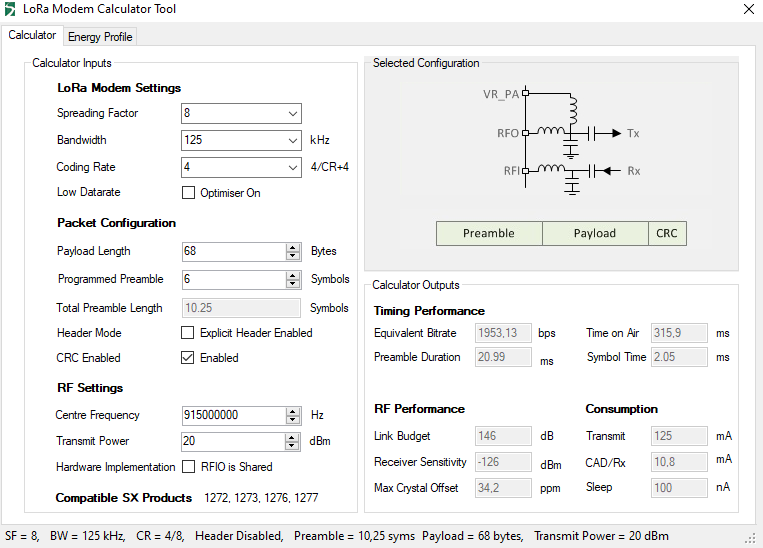
\includegraphics[scale=0.65]{figuras/calculo LoRa1.1.png}
  \caption{Cálculo transmissão LoRa pela Sentech. }
 { \footnotesize Fonte: Semtech - LoRa Modem calculator Tool} 
  \label{fig:calculo LoRa1}
\end{figure}


\begin{figure}[H]
  \centering
  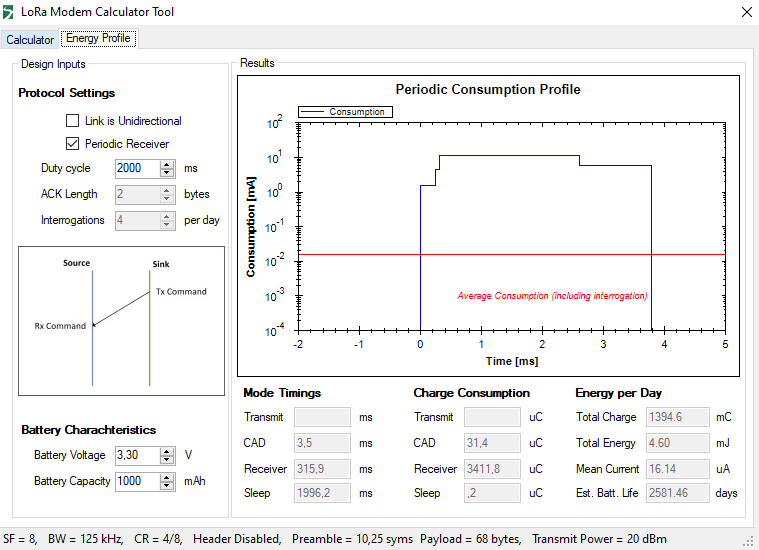
\includegraphics[scale=0.65]{figuras/calculo LoRa1.2.png}
  \caption{Cálculo transmissão LoRa pela Sentech. }
 { \footnotesize Fonte:Semtech - LoRa Modem calculator Tool} 
  \label{fig:calculo LoRa2}
\end{figure}


\section{Sensoriamento}

\par Sensores são dispositivos que possuem a função de detectar e responder com eficiência algum estímulo. Existem vários tipos de sensores que respondem a estímulos diferentes, como por exemplo: calor, pressão, movimento, luz e outros. Depois que o sensor recebe o estímulo, a sua função é emitir um sinal que seja capaz de ser convertido e interpretado pelos outros dispositivos \cite{mattede_Sensores_blog2020}.

\par Definidos os requisitos do projeto, sabe-se que será necessário o uso de sensores e transdutores para auxiliar a obter dados como pressão, temperatura, altitude, velocidade e localização geográfica (GPS) do foguete, e também do peso do foguete durante o abastecimento na sua base de lançamento. Para tal, serão utilizados apenas 3 sensores para ajudar na busca dessas variáveis.

\subsection{Altitude e Velocidade}

\par Para medição da pressão e da temperatura externa ao foguete durante o lançamento, foi escolhido o sensor de pressão e temperatura BMP280, visto na figura \ref{fig:sensor_pressao} \cite{datasheet_BMP280}.

\begin{figure}[H]
  \centering
  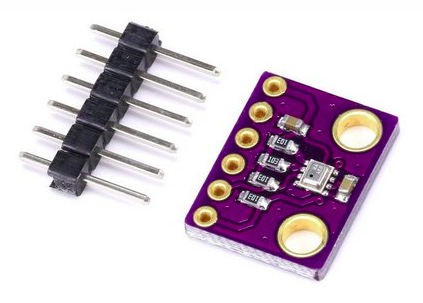
\includegraphics[scale=0.75]{figuras/BMP280.png}
  \caption{Sensor de pressão e temperatura BMP280 (Bosch). }
 { \footnotesize Fonte:\cite{figura_BMP280}} 
  \label{fig:sensor_pressao}
\end{figure}

\par Esse sensor mostrou-se o mais viável, pois, implementando-o com uso de determinadas bibliotecas, além dos dados de pressão (hPa) e temperatura (Graus Celsius), é possível, por meio da implementação de funções contidas em bibliotecas especificas, obter o cálculo da altitude (metros). Tais bibliotecas e suas equações são esclarecidas adiante.

\par O sensor BMP280 realiza medições de pressão com precisão de $\pm$ 1 hPa e temperatura com precisão de $\pm 1 ^\circ C $. Com essa precisão, é possível realizar medições de altitude com margem de erro de  $\pm$ 1 metro, efetuando a leitura entre 300 e 1100 hPa, o que corresponde à faixa de altitude de +9000 à -500 m \cite{cia_BMP280_2017}.

\par Em relação aos sensores existentes no mercado, o BMP280 foi o que melhor atendeu aos requisitos, pois ele é a versão mais atual e precisa dos modelos BMP180 e BM085. Também é de baixo consumo em relação aos sensores Mpx10dp e Mpx5700, possuindo melhor aplicabilidade.

\par Para a implementação do sensor, é necessário o uso de duas bibliotecas da Adafruit para o sensor BMP280 \cite{Adafruit}: a  \href{https://github.com/adafruit/Adafruit_BMP280_Library}{Adafruit\textunderscore Sensor.h} e a \href{https://github.com/adafruit/Adafruit_Sensor}{Adafruit\textunderscore BMP280.h}. Em ambientes que a Adafruit não pode ser implementada, a Bosh, fabricante do sensor, disponibiliza um código em C para a sua implementação (em \href{https://github.com/BoschSensortec/BME280_driver}{BME280\textunderscore driver}).

\par A biblioteca \href{https://github.com/adafruit/Adafruit_Sensor}{Adafruit\textunderscore BMP280.h} citada anteriormente é a biblioteca que disponibiliza as funções, em código C, que retornam as medidas de pressão e temperatura, e também a função que já realiza o cálculo da altitude, tais funções são:

	\begin{itemize}
	    \item float readPressure() -> Leitura da Pressao atmosférica
	    \item float readTemperature() -> Leitura da Temperatura
	    \item float readAltitude -> Leitura da Altitude (em metros, considerando nível do mar)
	\end{itemize} 

\par Os dados retornados por cada uma dessas funções são do tipo \textit{float}, portanto cada medida tem o dado do tamanho de 4 bytes.

\par A função \textit{readAltitude()} retorna o valor da altitude por meio da equação hipsométrica, vide equação \ref{eq_hipsometrica}. A equação hipsométrica estabelece que a distância vertical entre duas pressões na atmosfera é proporcional à temperatura média entre esses dois níveis de pressão \cite{hipsometric}.

\begin{center}
\begin{equation}
\label{eq_hipsometrica}
h=z_{2}-z_{1}=\frac{R_{d} \overline{T_{\nu}}}{g} \ln \left(\frac{p_{1}}{p_{2}}\right)
\end{equation}
\end{center}

Onde:
\begin{itemize}
    \item h é a variação da altitude, em que $z_{1}$ e $z_{2}$ são alturas geométricas nos níveis de pressão $p_{1}$ e $p_{2}$;
	\item $R_{d}$ é a constante de gás para ar seco, $8,3144 \frac{N*m}{mol*K}$ ;
	\item $\overline{T_{\nu}}$ a temperatura virtual média da camada;
	\item g é a aceleração gravitacional, $9.807 \frac{m}{s^{2}}$ .
\end{itemize} 

\par A equação hipsométrica é derivada da equação hidrostática e da lei dos gases ideais. Com essa fórmula a função calcula a altura h com, $p_{1}$ sendo a pressão atmosférica medida pelo sensor BMP280 e $p_{2}$ a pressão inicial da altura inicial, podendo ser a pressão a nível do mar (101,35 kPa) ou a do local.

\par Sabendo a altitude do foguete e obtendo a sua variação ao longo do tempo, este podendo ser medido pelo  \textit{clock} próprio do microcontrolador, considerando o tempo de recebimento de cada medida de altitude, é possível medir a velocidade do foguete em cada instante, por meio do cálculo da velocidade média, equação \ref{eq_vel_media}.

\begin{center}
\begin{equation}
\label{eq_vel_media}
V = \frac{\Delta S} {\Delta T} = \frac{h_{f} - h_{i}}{t_{f} - t_{i}}
\end{equation}
\end{center}

\par Onde:

\begin{itemize}
    \item V é a velocidade média do foguete durante o voo, em m/s;
	\item $\Delta$S é a variação de altitude do foguete durante o voo, em metros;
	\item $\Delta$T é a variação de tempo de subida do foguete durante o voo, em segundos;
	\item $h_{f}$ é a última medida coletada da altura do foguete;
	\item $h_{i}$ é a penúltima medida coletada da altura do foguete, esta inicia na altura h = 0 metros;
	\item $t_{f}$ é a medida do tempo em que foi coletado $h_{f}$;
	\item $t_{i}$ é a medida do tempo em que foi coletado $h_{i}$, está inicia em 0 segundos.
\end{itemize}

\par Ao contrário do cálculo da altitude, que é obtida por hardware dentro de rotinas implementadas em código C no microcontrolador, o processamento e cálculo da velocidade média do foguete, será realizado por software. A função do microcontrolador, nesse caso, será de enviar os dados de altitude para tal procedimento. 

\par Usando a comunicação I2C, a conexão das pinagens entre o sensor e o microcontrolador foi definida com o SDA e SCL do BMP280 conectados aos pinos D21 e D22 da ESP32 LoRa,respectivamente. Para comunicação, foram conetados o VDD e GND do BMP280 com os pinos 3V3 e GND da ESP32 LoRa respectivamente, conforme mostrado na figura \ref{fig:PINAGEM_BMP280}. 

\begin{figure}[H]
  \centering
  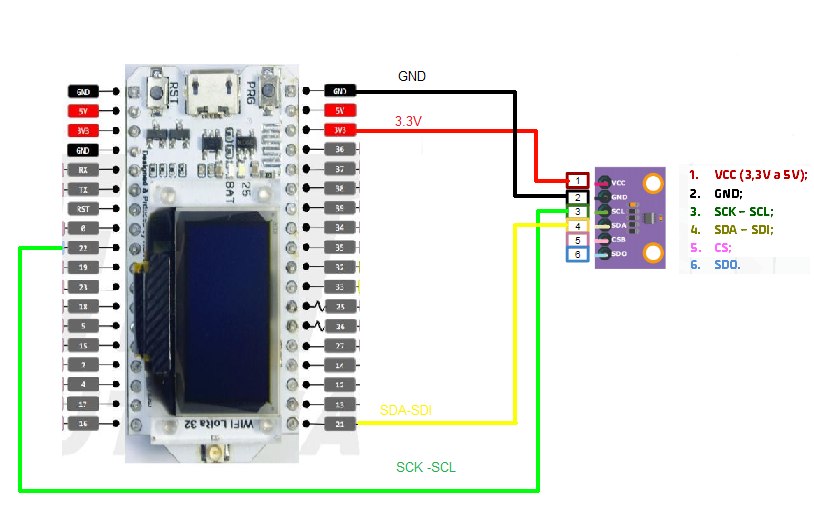
\includegraphics[scale=0.35]{figuras/PINAGEM_BMP280.png}
  \caption{Conexões entre sensor BMP280 e ESP32 LoRa - Protocolo I2C.} 
  {\footnotesize Fonte : Autor } 
  \label{fig:PINAGEM_BMP280}
\end{figure}

\subsection{Localização Geográfica (GPS)}

\par A sigla GPS significa Global Positioning System, o que em português quer dizer Sistema de Posicionamento Global. É uma tecnologia que utiliza satélites e dispositivos para fornecer informações sobre a localização no globo terrestre \cite{fisica_GPS_2020}.
\par A localização GPS será utilizada para obter a posição geográfica do foguete após sua aterrissagem, podendo também fornecer as coordenadas ao longo do lançamento para determinar a trajetória percorrida pelo foguete.
\par Foi definido para tal função o GY-NEO6MV2, figura \ref{fig:moduloGPS}, um módulo GPS composto por duas partes, a antena, responsável por captar as informações provindas dos satélites e o sistema de controle, responsável pelo processamento dos dados obtidos, por meio do microcontrolador interno NEO6 \cite{datasheet_GPS}.

\begin{figure}[H]
  \centering
  \includegraphics[scale=0.6]{figuras/moduloGPS.png}
  \caption{Módulo GPS GY-NEO6MV2 (uBlox). }
  {\footnotesize Fonte: \cite{figura_GPS}}
  \label{fig:moduloGPS}
\end{figure}

\par O módulo GPS GY-NEO6MV2 foi escolhido por ser de fácil utilização, realizando a comunicação por meio de comunicação serial, usando apenas 2 pinos (TX e RX), o que permite a comunicação com os mais diversos tipos de equipamentos e microcontroladores. Esse componente apresenta um consumo de corrente em média de 45 mA, enquanto o módulo similar, VK2828U7G5LF, consome em média 50 mA.

\par Para a aplicação com o módulo é necessário o uso de duas bibliotecas essenciais. A primeira é para a realizar a comunicação serial do microcontrolador com o módulo GPS, onde pode ser usada tanto a biblioteca \href{https://www.arduino.cc/en/Reference/softwareSerial}{SoftwareSerial.h} para usar a IDE do arduino, quanto a biblioteca \href{https://github.com/plerup/espsoftwareserial}{EspSoftwareSerial.h} como exclusivo da ESP32. A segunda (\href{https://github.com/mikalhart/TinyGPS}{TinyGPS.h}) contém todas as funções e comandos necessários para se comunicar com o módulo e acessar suas ferramentas.

\par Para GPS GY-NEO6MV2, com a vantagem da sua comunicação ser serial, a sua pinagem com a WiFi Lora ESP32 é bastante simples. Portanto, foi definida a conexão dos pinos de VCC e GND do módulo com os pinos 3V3 e GND da ESP32, para alimentação, e conectamos o TX e RX do módulo com os pinos de RX e TX da ESP32 LoRa, usando o procotolo UART de comunicação. A figura \ref{fig:PINAGEM_GPS} mostra as conexões entre os componentes.

\begin{figure}[H]
  \centering
  \includegraphics[scale=0.4]{figuras/PINAGEM_GPS.png}
  \caption{Conexões entre o GPS GY-NEO6MV2 e ESP32 LoRa - Protocolo UART.} 
  {\footnotesize Fonte : Autor } 
  \label{fig:PINAGEM_GPS}
\end{figure}


\subsection{Peso do foguete}
\label{Peso_do_Foguete}

\par Por meio do acompanhamento do peso do antes, durante e depois do abastecimento do foguete, será possível controlar e medir a quantidade de combustível contido em seu tanque. Para mensurar o peso do foguete, serão utilizadas duas células de carga. 

\par Uma célula de carga é um transdutor de força que converte a carga que atua sobre ele em uma saída elétrica mensurável. Embora existam vários tipos, as células de carga baseadas em sensores de deformação e tensão são as mais usadas \cite{omega_celulacarga}. 

\par Neste projeto, foi escolhida célula de carga de 50 kg, figura \ref{fig:celula_carga}, que atende o peso máximo do foguete, de 18.5 kg com o tanque de combustível cheio e 14.3 kg vazio (dados fornecidos pela CRT).

\begin{figure}[H]
  \centering
  \includegraphics[scale=0.5]{figuras/celula_carga.png}
  \caption{Célula de carga - 50 kg.}
  {\footnotesize Fonte: \cite{figura_celula}} 
  \label{fig:celula_carga}
\end{figure}

\par Este sensor é um \textit{Strain Gauge}, ou extensômetro, um sensor que é colocado na superfície de uma peça, responsável por medir a deformação diante da aplicação de um carregamento, onde no sensor há um fio resistivo, que altera sua resistência de acordo com o “alongamento” da superfície em que está colocado, gerando assim sinais elétricos que são interpretados por uma placa de aquisição, convertendo os valores em deformação \cite{strain_gauge}.

\par Uma ponte Wheatstone é um esquema de montagem de elementos elétricos que permite a medição do valor de uma resistência elétrica desconhecida, vide Figura \ref{fig:ponte_wheatstone}. Neste esquema elétrico são ligados quatro resistores, em dois diferentes ramos de um circuito, a uma bateria. Em seguida, esses ramos são conectados por um fio, que os leva a um galvanômetro. O galvanômetro serve como um indicador de corrente elétrica, assim, a resistência do resistor variável é alterada  até que o galvanômetro acuse a passagem de corrente nula. Quando a corrente que passa pelo galvanômetro é nula, não há diferença de potencial entre os ramos do circuito. Nessa situação, dizemos que a ponte de Wheatstone encontra-se em equilíbrio.

\begin{figure}[H]
  \centering
  \includegraphics[scale=0.6]{figuras/ponte_wheatstone.png}
  \caption{Circuito padrão de uma Ponte de Wheatstone.}
  {\footnotesize Fonte: \cite{ponte_wheatstone}} 
  \label{fig:ponte_wheatstone}
\end{figure}

\par Onde $i_{g}$ é a corrente no galvanômetro, $R_{X}$ é a resistência desconhecida e $R_{1}$, $R_{3}$, $R_{3}$ são resistências conhecidas. Na situação de equilíbrio, $i_{g} = 0$, o circuito mostrado na figura anterior pode ser usado para determinar com grande precisão a resistência elétrica do elemento resistivo RX. 
\par A célula de carga utilizada, é um sensor de meia-ponte da \textit{Wheatstone}, ou seja, utiliza uma meia-ponte de \textit{Wheatstone} com uma resistência de referência e um elemento sensor cuja resistência varia conforme a pressão aplicada, vide Figura \ref{fig:half_wheatstone}. Utilizando-se apenas uma célula de carga seriam necessários mais resistores para completar a ponte. Além disso, projetos com apenas uma célula de carga tendem a ter dificuldades para ajustes de calibração da célula.

\begin{figure}[H]
  \centering
  \includegraphics[scale=0.6]{figuras/half_wheatstone.png}
  \caption{Circuito Meia-Ponte de Wheatstone da Célula de Carga utilizada.}
  {\footnotesize Fonte: \cite{half_wheatstone}} 
  \label{fig:half_wheatstone}
\end{figure}

\par Portanto, considerando também que, além do foguete acima da balança, haverá toda uma estrutura para comportar a base do foguete, serão usadas duas células de cargas para fazer a balança, o que é o mais indicado: uma para medir compressão e outra para medir tensão (forças aplicadas em direções diferentes). Com duas células de carga, tem-se uma ponte de \textit{Wheatstone} completa.

\par Como o sinal enviado pelo transdutor é elétrico, precisa-se de um módulo conversor, que fará a conversão do sinal elétrico em sinal digital para possibilitar a leitura dos dados pelo microcontrolador. Para isso, será usado o módulo conversor A/D HX711, figura \ref{fig:conversorHX711}, um módulo amplificador e conversor A/D de 24 bits, utilizado para amplificar o sinal de dispositivos como células de carga, fazendo a interligação entre essas células e o microcontrolador, por meio da comunicação SPI \cite{avia_HX711}.

\begin{figure}[H]
  \centering
  \includegraphics[scale=0.6]{figuras/conversorHX711.png}
  \caption{HX711 - Módulo amplificador e conversor A/D de 24 bits.}
  {\footnotesize Fonte: \cite{figura_HX711}} 
  \label{fig:conversorHX711}
\end{figure}

\par O módulo HX711 foi projetado para pesar escalas e aplicações de controle industrial para interface diretamente com um sensor de ponte. O multiplexador de entrada seleciona o Canal A ou entrada diferencial B para o baixo ruído amplificador de ganho programável (PGA). O Canal A pode ser programado com um ganho de 128 ou 64,
correspondendo a uma entrada diferencial em escala real tensão de ± 20mV ou ± 40mV, respectivamente, quando uma fonte de 5 V é conectada à alimentação analógica do AVDD, pino de alimentação. O canal B tem um ganho fixo de 32. O regulador de alimentação Onchip elimina a necessidade para um regulador de alimentação externa fornecer energia para o ADC e o sensor. A entrada do \textit{Clock} é
flexível, pode ser de uma fonte de relógio externa, um
cristal, ou um oscilador on-chip que não requer nennhum componente externo. Não há necessidade de programação para os
registradores internos, todos os controles do HX711 são
através dos pinos \cite{avia_HX711}.

\par A Figura \ref{fig:bloco_H711}, mostra o diagrama de bloco de aplicação de uma balança típica com o HX711, dentro do bloco em azul, e a célula de carga, uma ponte de Wheatstone externa ao bloco. Em destacado em azul está o diagrama de bloco interno do módulo HX711.

\begin{figure}[H]
  \centering
  \includegraphics[scale=0.4]{figuras/blocoHX711.jpeg}
  \caption{Diagrama de blocos do módulo HX711 em aplicação típica de uma balança com uma célula de carga.} 
  {\footnotesize Fonte : \cite{avia_HX711} } 
  \label{fig:bloco_HX711}
\end{figure}

Aplicando ao presente projeto, a conexão das duas células de carga, formando a ponte completa de Wheatstone, e o módulo HX711, fica conforme mostrado na Figura \ref{fig:Circuit_balanca}.

\begin{figure}[H]
  \centering
  \includegraphics[scale=0.4]{figuras/Circuit_balanca.png}
  \caption{Circuito com 2 células de carga com conexões para o módulo HX711.} 
  {\footnotesize Fonte : \cite{half_wheatstone} } 
  \label{fig:Circuit_balanca}
\end{figure}

\par Para implementar a balança, a comunicação é feita do microcontrolador com o módulo conversor A/D e amplificador HX711. Para tal, foi definido o protocolo de comunicação I2C, sendo necessário o uso da biblioteca \href{https://github.com/bogde/HX711}{HX711.h}. Nessa biblioteca, a função a ser utilizada,  que retorna os dados do peso da balança é do tipo \textit{long}, ou seja, uma dado de 4 bytes.

\par As conexões entre o conversor e microcontrolador foram definidas da seguinte forma: para alimentação, o VDD e GND do HX711 conectados nos pinos 5V e GND da ESP32 Lora, respectivamente, para comunicação I2C, o DT e SCK do HX711 conectados nos pinos D23 e D17 da ESP32 LoRa. A figura \ref{fig:PINAGEM_balanca} mostra as pinagens realizadas.  

\begin{figure}[H]
  \centering
  \includegraphics[scale=0.4]{figuras/PINAGEM_BALANCA.png}
  \caption{Conexões entre Hx711 e ESP32 LoRa - Protocolo I2C.} 
  {\footnotesize Fonte : Autor } 
  \label{fig:PINAGEM_balanca}
\end{figure}

\subsection{Especificações dos sensores}

\par A tabela \ref{tab:sensores} apresenta os dados das principais especificações dos sensores citados acima.

\begin{center}
\begin{table}[H]
\centering
\begin{tabular}{ |m{2cm}|m{2cm}|m{2.5cm}|m{2.5cm}|m{2.5cm}|m{2.5cm}| } 
\hline

\textbf{ Sensor }&\begin{center}
\textbf{ Tensão de Operação} \end{center}& \textbf{Consumo de corrente }& \textbf{Comunicação} & \begin{center}\textbf{Taxa de transmissão} \end{center} & \begin{center}\textbf{Formato dos Dados}\end{center}\\ 
 \hline
 
 BMP280 & 1.71 - 3.6V & 3.6 $\micro$uA @ 1 Hz (umidade, pressão e temperatura) & 
I2C e SPI & I2C (até 3.4 MHz e SPI (3 e 4 fios, até 10 MHz) & unsigned 20-bit (pressão e temperatura) unsigned 16-bit (umidade)\\
  \hline
Célula de carga 50kg & 5 -10V & Resistência de entrada e saída ($\ohm$): 1000 ± 50 & - & - & - \\
  \hline
 Módulo Hx711 & 4.8 - 5.5V & 1.5mA & SPI & 10 - 80 MHz & 24 bits em complemento de 2 \\ 
  \hline
 Módulo GPS GY-NEO6MV2 & 3 - 5V & 10mA – 100 mA & Serial UART e SPI & 9600 bps (UART baud rate) e 100 kbit/s & - \\ 
 \hline 

\end{tabular}
\caption{Especificações principais dos componentes do sensoriamento.}
\label{tab:sensores}
\end{table}
\end{center}


\section{Central de controle}

\par A central de controle será o ponto de acesso do usuário com os dados e comandos vindos da base de lançamento e do foguete. Um exemplo de estação pode ser visto na figura \ref{fig:DroneStation}. 

\begin{figure}[H]
  \centering
  \includegraphics[scale=0.4]{figuras/DroneGroundStation.jpg}
  \caption{Estação de controle de solo.}
  {\footnotesize Fonte : \cite{AeroExpo}} 
  \label{fig:DroneStation}
\end{figure}


\par A solução proposta para essa interface do usuário foi seguindo esse modelo de maleta, que possui uma tela, um teclado.

\subsection{Interface do usuário}

\par A tela escolhida pode ser vista na figura \ref{fig:Tela}. Essa tela possui um tamanho de 9 polegadas e uma resolução máxima de 1600x1200. 


\begin{figure}[H]
  \centering
  \includegraphics[scale=0.6]{figuras/TELAPI2.png}
  \caption{Tela da interface do usuário. }
  {\footnotesize Fonte : \cite{figura_Tela} } 
  \label{fig:Tela}
\end{figure}

\par Para a chegada dessa definição, pesquisas foram feitas e percebeu-se que geralmente telas menores, cinco e sete polegadas, possuem sensibilidade ao toque o que além de não agregar mais valor em nosso produto, dificultaria no dimensionamento da bateria dado a maior necessidade de potencia desse tipo de tela. Outro ponto levado em consideração é a questão da troca que existe entre o tamanho da tela e seu gasto energético. Precisava-se de uma tela grande o suficiente para a boa visualização dos dados, porém que fosse portátil e que consumisse pouca carga da bateria. Assim a escolha da tela com as características mencionadas anteriormente é justificada.

\par Para que o usuário interaja com essa tela, foi pensado em dois tipos de soluções. A primeira seria colocar todos os comandos em botões e chaves, e a segunda realizar os comandos por meio de um mini teclado. Optou-se pelo o uso do teclado, devido a possibilidade de maior interatividade com a aplicação de \textit{software} e facilidade para futuras atualizações no projeto. 

\par O modelo de teclado portátil escolhido pode ser visto na figura  \ref{fig:Teclado}. Esse teclado possui dimensões de 200x126x6,2 mm e um peso de 200g.





\begin{figure}[H]
  \centering
  \includegraphics[scale=0.5]{figuras/TecladoPI2.png}
  \caption{Teclado da interface do usuário.}
  {\footnotesize Fonte : \cite{figura_Teclado}} 
  \label{fig:Teclado}
\end{figure}

\subsection{ \textit{Single Board Computer}}

\par Para a melhor escolha da placa utilizada no projeto, foi montada a seguinte tabela, na figura \ref{fig:comparacaoMicro}. Essa tabela foi levada aos grupos de \textit{software} e de energia para o debate entre capacidade de processamento e custo energético.

\begin{figure}[H]
  \centering
  \includegraphics[scale=0.8]{figuras/SBCcomparacao.png}
  \caption{Tabela de comparação de \textit{single board computers}. Fonte : Autor } 
  \label{fig:comparacaoMicro}
\end{figure}

\par Após algumas reuniões, ficou decidido que se usaria a raspberry pi 3B+ no projeto. Porém, conforme as  \textit{sprints} foram passando, percebemos juntamente com o grupo de software que seria necessário mais capacidade de processamento para os algoritmos que seriam implementados. Um novo alinhamento geral foi feito e a escolha que melhor atenderia essa demanda de processamento seria o uso de uma Jetson Nano Developer Kit da Nvidia, mostrado na figura \ref{fig:Nvidea}. 

\begin{figure}[H]
  \centering
  \includegraphics[scale=0.5]{figuras/NvideaPI2.png}
  \caption{Nvidea Jetson Nano Developer Kit. } 
  {\footnotesize Fonte : \cite{Nvidia_Nano} } 
  \label{fig:Nvidea}
\end{figure}

\par Apesar do detrimento causado no dimensionamento da bateria, essa placa foi escolhida devido a sua maior  capacidade de processamento de algoritmos mais pesados, assim suprindo a demanda encaminhada pela equipe de \textit{software}.

\par Juntamente com a equipe de energia foi construído um diagrama de blocos das interligações dos componentes, o mesmo pode ser visto  na figura \ref{fig:CentraldeCOntrole}. Visto as colaborações necessárias entre os dois grupos com relação ao dimensionamento da bateria, por parte da energia, e o consumo de potência de cada componente por parte da eletrônica. 


\begin{figure}[H]
  \centering
  \includegraphics[scale=0.6]{figuras/Maleta_Diagrama.jpg}
  \caption{Diagrama Central de Controle. } 
  {\footnotesize Fonte : Autor } 
  \label{fig:CentraldeCOntrole}
\end{figure}

\section{Calibração}

\par Calibração é operação que estabelece, sob condições especificadas, num primeiro passo, uma relação entre os valores e as incertezas de medição fornecidos por padrões e as indicações correspondentes com as incertezas associadas; num segundo passo, utiliza esta informação para estabelecer uma relação visando a obtenção de um resultado de medição a partir de uma indicação. \cite{VIM_CALIBRACAO}.

\par Dentre os sensores utilizados na base de lançamento e no foguete, apenas as células de cargas da balança são transdutores necessários de calibração, os demais sensores já possuem calibração de fábrica, onde geralmente seus coeficientes de calibragem ficam armazenados em ROM.

\par Para calibrar a balança, após a montagem com as duas células de carga 50 Kg e o módulo conversor HX711, será executado uma rotina de ajuste do sistema de medição em código C no microcontrolador ESP32 LoRa. De acordo com o Vocabulário Internacional de Metrologia Legal (VIML) o ajuste de um sistema de medição é conjunto de operações efetuadas num sistema de medição, de modo que ele forneça indicações prescritas correspondentes a determinados valores de uma grandeza a ser medida. 

\par Através do programa executado deve ser encontrado um valor aferido  denominado como Fator de Ajuste para  ser inserido no programa de medição da Balança com o conversor, e assim a calibração seja realizada.

\par O programa de ajuste fará uso da biblioteca \href{https://github.com/bogde/HX711}{HX711.h}, onde um objeto de peso conhecido deve ser lido pela balança, e a média dos valores retornados deve ser dividido pelo valor do peso real do objeto em KG, obtendo o fator de ajuste, que deve ser inserido como parâmetro da função “scale.set\textunderscore scale()” importada da biblioteca mencionada. Com esse fator de ajuste setado, obtém-se a calibração da balança, medindo então o do peso real do objeto \cite{CALIBRACAO_tutorial}.

\par A figura \ref{fig:Calibracao_balanca} apresenta o fluxograma do algoritmo de ajuste e calibração dos sensores da balança.

\begin{figure}[H]
  \centering
  \includegraphics[scale=0.6]{figuras/Algoritmo de Calibração da Balança.png}
  \caption{Diagrama do algoritmo de calibração da balança } 
  {\footnotesize Fonte : Autor } 
  \label{fig:Calibracao_balanca}
\end{figure}

Convém ressaltar que foi escolhido para os dados de peso medidos pela balança, uma precisão de 3 casas decimais. Esta precisão é definida como um parâmetro setado em uma função contida na biblioteca \href{https://github.com/bogde/HX711}{HX711.h}.

\section{Integrações}
\subsection{Diagrama de blocos do Abastecimento}
\par Apos reuniões com a equipe de estrutura e com a CRT, foram levantados os requisitos para o abastecimento do foguete de forma mais especifica. Foi criado um diagrama lógico para melhor entendimento do procedimento, figura \ref{fig:Abastecimento do fohuete}, maiores detalhes estão apresentados no capitulo \ref{abastecimento}. Assim, foi possível a equipe estrutural definir quais motores se enquadram para cada válvula do sistema.
\par É necessário um conjunto de 3 motores para a parte externa do foguete, um para a válvula 1 responsável por abrir o cilindro do combustível, um para a válvula 2 que é responsável por despressurizar a mangueira após a conclusão do abastecimento,um para o desacoplamento do engate rápido e o ultimo para o acionamento da ignição, sendo que estes dois ultimos seriam acionados por um modulo de dois relés SRD‑05VDC‑SL‑C, por necessitarem se movimentarem somente em uma direção linear tanto no desengate quanto na ignição, diferentemente dos outros dois citados anteriormente, que necessitam se movimentarem nos dois sentidos (horário e anti-horário, para abertura e fechamento das válvulas), fazendo-se necessário usar o modulo L298N, que é uma ponte H dupla.  
\par Já na parte interna do foguete, existem dois atuadores, que seriam acionados também de modo remoto: a válvula 4, que é uma válvula solenoide, responsável pelo controle da pressão do tanque do foguete, ou seja, ela fica abrindo e fechando a fim de estabilizar a pressão interna do foguete liberando gases internos durante o abastecimento; e a válvula 5, que é aberta na ignição, expulsando o óxido nitroso do tanque do foguete em direção à câmara de combustão. Ambas serão abertas em um só sentido; portanto, foi proposto usar um módulo de dois relés SRD‑05VDC‑SL‑C para seu acionamento pelo microcontrolador interno do foguete.
     


\begin{figure}[H]
  \centering
  \includegraphics[scale=0.35]{figuras/abastecimento .png}
  \caption{ \href{https://drive.google.com/file/d/1EhMWyoD2Ml5I2vsLA0MbNOR8LxuCMmC5/view?usp=sharing}{ Diagrama logico do abastecimento foguete}. } 
  {\footnotesize Fonte : Autor } 
  \label{fig:Abastecimento do fohuete}
\end{figure}

\subsection{Acionamento eletrônico das válvulas externas e ignição}

\par As válvulas externas terão o seu acionamento controlado pelo microcontrolador ESP32 LoRa contido na base de lançamento do foguete, o qual também atua no controle da balança. Por meio dele serão enviados comandos de acionamento para fechar e abrir as válvulas externas durante o processo de abastecimento do foguete.

\par De acordo com informações obtidas do grupo de estrutura, serão necessários 3 adaptadores externos, sendo 2 válvulas esféricas que atuam no tanque de combustível e mangueira, e 1 atuador para desengate rápido, onde é necessário apenas o desengate remoto, pois o engate é manual. 

\par As válvulas esferas serão acionadas por meio de dois motores, um para cada válvula, onde o microcontrolador fará o seu acionamento por meio de uma Ponte H, enviando comandos para girar o motor em sentido horário ou anti-horário, ou seja, abrir ou fechar a válvula. A solução mecânica entre motores e válvulas é detalhado na estrutura.

\par De acordo com a estrutura, os motores usados para controle das válvulas esferas são do modelo Mabuchi 8d 12V. Esse motor é alimentado com 12V, com um consumo de corrente de 1,3A e torque de 9,12 N.m / 93 Kg. Para controle dos motores será necessário o uso de ponte H para realizar abertura e fechamento, controlando o sentido de rotação dos motores. 

\par A ponte H é um circuito que serve para variar o sentido da corrente em uma determinada carga, bem como controlar sua potência. A figura \ref{fig:PonteH_circuito} apresenta o circuito típico de uma ponte H.

\begin{figure}[H]
  \centering
  \includegraphics[scale=0.3]{figuras/ponteH_circuito.png}
  \caption{ Circuito típico de uma ponte H.} 
  {\footnotesize Fonte : \cite{PonteH_Teoria}} 
  \label{fig:PonteH_circuito}
\end{figure}

\par Com base nas especificações dos motores, foi escolhido o Driver Motor Ponte H L298n, figura \ref{fig:PonteH_modulo}, para controle destes. Esse módulo possui tensão de operação de 4 a 35V, com corrente de operação máxima de 2A por canal (ou 4A máxima), tensão lógica de 5V, corrente lógica de 0 a 36mA e potência máxima de 25W \cite{PonteH_Datasheet}. O grande benefício desse módulo é que, com ele, é possível controlar dois motores ao mesmo tempo e, se necessário, controlar a velocidade deles, atuando no PWM do sinal enviado.

\begin{figure}[H]
  \centering
  \includegraphics[scale=0.4]{figuras/ponteH_modulo.jpg}
  \caption{ Driver Motor Ponte H L298n.} 
  {\footnotesize Fonte : \cite{PonteH_mod}} 
  \label{fig:PonteH_modulo}
\end{figure}

\par Como o módulo da ponte H trabalha com tensão lógica de 5V, é necessário o uso de um conversor lógico de 3.3V (tensão lógica dos pinos da ESP32 LoRa) para 5V. Para tal, foi escolhido o Módulo Conversor Nível Lógico 5V/3.3V - Bidirecional (4 Canais), figura \ref{fig:CONV_LOGICO}. Esse conversor é capaz de elevar tensões de nível lógico de 3,3V para 5V, e isso de forma totalmente segura, possuindo 4 canais independentes que permitem a conversão de sinal. Entretanto, o conversor não é capaz de funcionar com sinais analógicos. A placa necessita de alimentação das duas tensões (alta tensão e baixa tensão) com que seu sistema estiver trabalhando \cite{Conversor_logico}.

\begin{figure}[H]
  \centering
  \includegraphics[scale=0.4]{figuras/conv_logico.jpeg}
  \caption{ Módulo Conversor Nível Lógico 5V/3.3V - Bidirecional (4 Canais)} 
  {\footnotesize Fonte : \cite{Conv_logico}} 
  \label{fig:CONV_LOGICO}
\end{figure}

\par Ressalta-se que na parte externa ao foguete, tem-se também o engate rápido, cuja solução mecânica não faz parte do escopo do projeto e sim da CRT. Todavia, apenas o acionamento eletrônico do seu desacoplamento do foguete faz parte do escopo da eletrônica, devido a necessidade de fazê-lo de maneira remota. 

\par Para tal, a solução adotada pela CRT é que o desacoplamento do engate seja feito com o auxílio de um motor de vidro elétrico universal, modelo Mabuchi 8d 12v, o mesmo modelo utilizado para as válvulas esferas. O desacoplamento deve ocorrer quando o motor for acionado, onde um cabo de aço preso ao engate irá enrolar ao eixo no motor, puxando a mangueira para fora do engate.

\par Por fim, tem-se externo ao foguete a resistência de ignição, um fio ignitor de Níquel Cromo (Ni-Cr) com resistência calculada em 2,23 Ohms, a qual deve ser acionada pelo microcontrolador da base, assim que o comando for enviado para propulsão do foguete. O acionamento da ignição é realizado quando uma corrente de 5,38A passa pela resistência, alimentada pela bateria de 12V e esta encandeia alcançando a temperatura de 300°C, fazendo o propelente entrar em combustão.

\par Uma vez que o motor de desengate não precisará inverter o sentido de rotação, e a resistência de ignição é acionada pela passagem de uma corrente direta, ou seja, tensão DC; não é necessário o uso de ponte H, portanto, para realizar ambos acionamentos, será utilizado um módulo  Módulo Relé 5V 2 Canais modelo SRD-05VDC-SL-C, figura \ref{fig:RELE_2CHANNEL}. Esse relé possui 2 canais, um para o motor de desengate e outro para a resistência de ignição, possui tensão de operação de 5V, com um consumo de corrente típica de 15~20mA e possui capacidade na faixa de (30 VDC a 10A) ou (250VAC a 10A), o que atende a especificação do motor Mabuchi e da resistência de ignição \cite{rele_two}.

\begin{figure}[H]
  \centering
  \includegraphics[scale=0.3]{figuras/RELE_2CHANNEL.jpg}
  \caption{ Módulo Relé 5V 2 Canais modelo SRD-05VDC-SL-C} 
  {\footnotesize Fonte : \cite{rele_photo}} 
  \label{fig:RELE_2CHANNEL}
\end{figure}

\par A conexão dos módulos atuadores das válvulas, do desengate e da ignição no microcontrolador é estabelecido conforme esquema da figura \ref{fig:base_valvulas}.

\begin{figure}[H]
  \centering
  \includegraphics[scale=0.5]{figuras/BASE_VALVULAS.png}
  \caption{ Conexões entre atuadores externos e microcontrolador da base de lançamento. } 
  {\footnotesize Fonte : Autor}
  \label{fig:base_valvulas}
\end{figure}

\par Onde, M1 é o motor do desengate remoto, M2 é a resistência de ignição e M3 e M4 são os motores de abertura e fechamento das válvulas esferas do cilindro de combustível e mangueira, respectivamente.

\subsection{Acionamento eletrônico das válvulas internas}

\par As válvulas internas do foguete, serão controladas e acionadas pelo microcontrolador ESP32 LoRa presente no foguete, o qual também faz o controle dos sensores de pressão e temperatura e módulo GPS.

\par Uma vez que é necessário acionar com precisão a válvula 4, ou seja, uma válvula solenoide, não é necessário o uso de ponte H. Portanto, para realizar o acionamento desta, será utilizado um relé que atende a necessidade de ficar acionando a válvula solenoide de tempo em tempos, e a outra válvula interna é do tipo esférica que será aberta somente uma vez também será acionado por relé,assim foi definido o uso do Módulo Relé 5V 2 Canais modelo SRD-05VDC-SL-C, figura \ref{fig:RELE_2CHANNEL}, com as configurações supracitadas anteriormente. Esse relé possui 2 canais, um para a válvula solenoide e um para o motor da válvula 5 controlados pela ESP32-LoRa de dentro do foguete que mandará os sinais de controle para o modulo de relés e pode ser observado melhor no diagrama esquemático do circuito interno do foguete na figura \ref{fig:Diagrama esquematico do circuito interno do foguete}.

\subsection{Comunicação hardware e software}

\par Visto que um dos maiores objetivos do projeto é a realização da telemetria com os dados vindos do foguete,este tópico tratará a maneira pela qual será realizada a comunicação entre o \textit{hardware} e a aplicação de \textit{software} e também como o dado trafegará em todo o sistema.

\par Para exemplificar de forma mais clara o caminho e os protocolos usados, a explicação será feita pro meio do apêndice \ref{diagrama_sequencia}, onde juntamente com a equipe de \textit{software} foi desenvolvido um diagrama de sequência tratando os processos que envolvem esta comunicação.


%\begin{figure}[H]
%  \centering
%  \includegraphics[scale=0.7]{figuras/Fluxo_dados.jpg}
%  \caption{ Fluxo de dados} 
%  {\footnotesize Fonte : Autor} 
%  \label{fig:FLuxoDados}
%\end{figure}

\par Todos os comandos são inseridos pelo usuário por meio do teclado, então o \textit{software} do sistema informa essas ações via comunicação serial para o microcontrolador da maleta, pois ambos estão conectados via USB. Assim que o comando chegar neste primeiro microcontrolador, ele é transmitido para a base do foguete ou para o próprio foguete, via comunicação LoRa, dependendo do processo que esta sendo executado.

A partir do momento em que a missão de lançamento é iniciada pelo usuário figura \ref{fig:Diagrama_sequencia_missao}, sera estabelecido uma comunicação entre os microcontroladores da maleta e da base, esta comunicação durará até a faze da ignição do foguete. Com essa comunicação estabelecida o primeiro comando a ser executado é do abastecimento do foguete \ref{fig:Diagrama_sequencia_abastecimento}. Para este comando é necessário que sejam enviados os dados do peso do foguete vazio e o peso do foguete cheio, assim que esses dados forem inseridos eles serão transmitidos para o microcontrolador da base e uma confirmação de inicio de abastecimento será retornada. Durante o abastecimento o dado do peso atual do foguete será transmitido para a interface do usuário até que peso esperado seja atingido, quando uma confirmação será enviada indicando o termino do processo.

O próximo comando é o do desengate da mangueira de abastecimento figura \ref{fig:Diagrama_sequencia_desengate}. Assim que este comando for aplicado pelo usuário, uma confirmação de inicio de desengate será retornada do hardware para o software e, como dito anteriormente, o comando será enviado para o microcontrolador da base, que executará  a despressurização da mangueira e posteriormente o acionamento do motor responsável pelo  desengate.Após o processo uma confirmação de termino do desengate será retornada.

Seguindo o processo, o próximo comando trata-se do inicio da ignição e é durante este comando em que ocorre a troca de comunicação do sistema da base para o o microcontrolador do foguete. Assim que este comando é acionado o microcontrolador da base aciona o ignitor e a troca da comunicação, citada anteriormente, é realizada. A partir do momento em que a comunicação com o foguete for estabelecida a válvula de lançamento será aberta, fazendo com que o foguete seja lançado.A partir deste momento o usuário receberá uma mensagem de termino da ignição e passará a receber todas as informações dos sensores do foguete.  







\section{Diagramas e esquemáticos}

\par Com a definição da solução e dos componentes da base de lançamento, foi criado o esquemático do circuito integrado, com detalhamento de pinos, conexões e módulos utilizados. A figura \ref{fig:Diagrama esquematico do circuito interno da base de lancamento} apresenta o circuito integrado da base de lançamento, com os componentes da balança e os módulos dos atuadores externos, assim como bornes para os motores. Na figura \ref{fig:Diagrama esquematico do circuito interno do foguete}, encontra-se o diagrama esquemático, o detalhamento das conexões do sensoriamento interno do foguete, assim como a parte de controle das válvulas internas. Na figura \ref{fig:Diagrama esquemático do circuito da central de controle do usuário}, por sua vez, tem-se o esquemático com as conexões na base central de comando entre a ESP32 Wifi Lora e a Jetson e outros periféricos. Os esquemáticos foram feitos utilizando as ferramentas do \textit{software} EasyEDA ,assim como o projeto de suas PCIs.

\begin{figure}[H]
  \centering
  \includegraphics[scale=0.35]{figuras/PDFs/final eletronica/Schematic_base de lançamento.pdf}
  \caption{Diagrama esquemático do circuito interno da base de lançamento.} 
  {\footnotesize Fonte:Autor} 
  \label{fig:Diagrama esquematico do circuito interno da base de lancamento}
\end{figure}

\begin{figure}[H]
  \centering
  \includegraphics[scale=0.35]{figuras/PDFs/final eletronica/Schematic_Esquemático foguete.pdf}
  \caption{Diagrama esquemático do circuito interno do foguete. } 
  {\footnotesize Fonte:Autor} 
  \label{fig:Diagrama esquematico do circuito interno do foguete}
\end{figure}

\begin{figure}[H]
  \centering
  \includegraphics[scale=0.35]{figuras/PDFs/final eletronica/Schematic_maleta final.pdf}
  \caption{Diagrama esquemático do circuito da central de controle do usuário.} 
  {\footnotesize Fonte:Autor} 
  \label{fig:Diagrama esquemático do circuito da central de controle do usuário}
\end{figure}

\section{Placa de circuito impresso}

\par Para melhor funcionamento  e durabilidade do circuito, é necessária a criação do desenho de placa de circuito impresso, conhecido como PCI, que é gerido por regras que visam garantir a qualidade do funcionamento do circuito IPC-2221B \cite{IPC-2221}, visando a disposição dos componentes para melhor acomodação mecânica e eletromagnética, a fim de evitar interferências no circuito.
\par Basicamente, é constituída por uma base de um material isolante, geralmente fenolite ou fibra de vidro, revestida por uma fina camada de cobre na sua superfície, onde ocorre as ligações entres os componente eletrônicos que podem ser do tipo PTH ou SMD\cite{pci}. 

\par As placas utilizadas nesse projeto serão feitas de modo a acomodar componentes do tipo PTH, ou seja, componentes que serão inseridos na placa através de um furo denominado de pads, sendo necessário uma acurácia para não errar no distanciamento dos furos, evitando assim mal posicionamento dos componentes eletrônicos.
\par Outro levantamento importante que é necessário fazer no projeto de uma PCI é a largura das trilha, que são responsáveis pelas conexões elétricas entre os componentes, a qual é determinada pela corrente que irá passar pela trilha e pela espessura da trilha de cobre  e a temperatura \cite{ TecnicasdeProjetosPCI}. Os cálculos das trilhas foram feitos no site \href{https://pcbbrasil.com.br/calculo-trilha-pcb.php}{PCBBRASIL} que segue os critérios da norma IPC-2221B para confecção de placas de circuito impresso.
\par Para a confecção da placa de circuito impresso foi gerado o arquivo Gerber de cada placa de circuito impresso, sendo gerado um arquivo em formato ZIP disponível em \href{https://drive.google.com/drive/folders/1P1pQGE_zuSLOB5qd8zfESWqLDwtyoRKd?usp=sharing}{ Arquivos Gerber}. Para a visualização dos arquivos Gerber é necessário a utilização de um programa de prototipagem de placas de circuito impresso ou um visualizador desse tipo de arquivo disponível para \href{https://sourceforge.net/projects/gerbv/files/}{ \textbf{download}} no site do programa utilizado para o projeto EasyEda.

\subsection{Circuito interno do foguete}
\par Na figura \ref{fig:Diagrama esquematico do circuito interno do foguete}, está representado o circuito interno do foguete. Assim, na figura \ref{fig:PCIFOGUETE}, encontra-se o  projeto mecânico da placa de circuito impresso com as dimensões para sua fabricação. Foram adicionados cinco buracos na PCI no intuito de facilitar sua fixação dentro do foguete com parafusos de diâmetro de 5mm. Na figura \ref{fig:PCB_FOGUETE}, por sua vez, é apresentado o modelo 3D da PCI com com o sistema de alimentação à esquerda da placa, separado dos outros componentes a fim de evitar interferência eletromagnética no restante da placa. Foi adicionado a essa placa esse sistema para garantir a tensão adequada para os componentes. 
\par A placa a ser produzida possui espessura padrão de 1,6mm, com tolerância nominal de $\frac{+}{-}$ 0,13mm. Nessa PCB específica, são utilizadas duas camadas de cobre para as trilhas; portanto, serão feitas trilhas tanto na \textit{Top Layer} quanto na \textit{Bottom Layer}, ou seja, \textit{multilayer}, garantindo uma melhor distribuição das trilhas. Por ser um módulo que vai dentro do foguete, inicialmente foi pensado em usar componentes do tipo PTH e a plaquinha de desenvolvimento da ESP32Lora, da Heltec, pois não são feitos muitos lançamentos. A ideia é utilizar primeiramente uma PCB nesse formato para testes e melhorias no projeto, antes de confeccionar uma placa mais enxuta com componentes SMD. 
\par Para essa versão inicial das placas de circuito impresso, seriam feitas de fenolite (FR2), que é um material mais barato para a confecção e quando tiver os componentes testados será feito em material de vibra de vidro(FR4)\cite{CONCEITOpci}.

\begin{figure}[H]
  \centering
  \includegraphics[width=\textwidth]{figuras/PDFs/final eletronica/PCB_PCB_interna do foguete.png}
  \caption{Dimensões da PCI do circuito interno do foguete.} 
  {\footnotesize Fonte : Autor } 
  \label{fig:PCIFOGUETE}
\end{figure}

\begin{figure}[H]
  \centering
  \includegraphics[scale=0.4]{figuras/PDFs/final eletronica/foguete_top.png}.
    \includegraphics[scale=0.4]{figuras/PDFs/final eletronica/foguete_bottom.png}
  \caption{PCI do circuito interno do foguete.} 
  {\footnotesize Fonte : Autor } 
  \label{fig:PCB_FOGUETE}
\end{figure}


\subsection{Circuito na base de lançamento}
\label{sec:base_de_lancamento}

Objetivando reduzir o número de fios e cabos utilizados no circuito da base de lançamento, assim como obter a menor ocupação de volume de circuitaria e componentes, foi criado o modelo de PCI com base no circuito integrado citado na figura \ref{fig:Diagrama esquematico do circuito interno da base de lancamento}. Foi optado o modelo \textit{Bottom Layer} para as trilhas da PCI, ou seja, contém apenas uma camada de cobre.

A figura \ref{fig:PCB_BASE_LANCAMENTO_DES} mostra o desenho da PCI, junto com suas cotas de dimensões definidas, que foram de 88mm x 109mm. Os buracos nos cantos da PCB, com diâmetro de 4mm e distâncias das bordas de 3mm, servem pra fixação da placa na estrutura da base.

\begin{figure}[H]
  \centering
  \includegraphics[width=\textwidth]{figuras/PDFs/final eletronica/PCB_BASE_FINAL.png}
  \caption{ Dimensões da PCI do circuito interno da base de lançamento. } 
  {\footnotesize Fonte : Autor } 
  \label{fig:PCB_BASE_LANCAMENTO_DES}
\end{figure}

A figura \ref{fig:PCB_BASE_LANCAMENTO} apresenta a visão frontal da PCI, onde é possível visualizar a posição dos componentes, tais como encaixes dos pinos e os bornes dispostos nas extremidades, e a visão traseira da PCI, onde se encontra a camada de fundo (\textit{Bottom Layer}), com as trilhas do circuito.

\begin{figure}[H]
  \centering
  \includegraphics[scale=0.4]{figuras/PDFs/final eletronica/BASE_TOP.png}
    \includegraphics[scale=0.4]{figuras/PDFs/final eletronica/BASE_BOTTOM.png}
  \caption{PCI do circuito interno da base de lançamento } 
  {\footnotesize Fonte : Autor } 
  \label{fig:PCB_BASE_LANCAMENTO}
\end{figure}

\subsection{Circuito na base de controle central}

A ideia dessa PCI é reduzir o número de cabos utilizados dentro da maleta do usuário.
De acordo com o espaço e a disposição dos componentes mostrado na figura  \ref{fig:Disposicao dos Componentes} e na figura \ref{fig:PCB_controle} pensou-se em fazer uma placa de modo que os módulos sejam encaixados nas laterais da PCI. Para isso foi verificado todos desenhos técnicos dos componentes, mapeando então os conectores  por meio dessas medidas fornecidas pelo fabricante. Os conectores precisarão ser do tipo macho para que o encaixe seja realizado. Isso traz vantagens: caso algum módulo sofra dano, bastará  desconectá-lo e realizar a troca.

\begin{figure}[H]
  \centering
  \includegraphics[scale=0.5]{figuras/PCB_Maleta.png}
  \caption{ Dimensões da PCI do circuito da central de controle.} 
  {\footnotesize Fonte : Autor } 
  \label{fig:PCIMaleta}
\end{figure}

\begin{figure}[H]
  \centering
  \includegraphics[scale=0.4]{figuras/PDFs/final eletronica/maleta_top.png}
    \includegraphics[scale=0.4]{figuras/PDFs/final eletronica/maleta_bottom.png}
  \caption{PCI do circuito interno do foguete. } 
  {\footnotesize Fonte : Autor } 
  \label{fig:PCB_controle}
\end{figure}

\chapter{Energia}

\par A solução de energia do projeto consiste no dimensionamento de baterias que atendam às especificações e requisitos do sistema, tanto dos dispositivos eletrônicos quanto do sistema de ignição e lançamento. Além disso, é projetado um carregador de bateria para tornar contínuo o uso do equipamento.

\par Para dimensionar o consumo do sistema, foi observado o gasto energético dos componentes eletrônicos, levando em conta que o projeto precisa de uma autonomia de, no mínimo, duas horas de uso sem a possibilidade de ter como fonte de energia a rede elétrica.

\par Anteriormente, ao dimensionar o sistema de alimentação do projeto, foi definido que seria utilizada apenas uma bateria que alimentasse todos os componentes. Porém, ao avaliar melhor as necessidades do projeto, em especial a distância de segurança (500 m) entre o usuário e a base de lançamento do foguete, optou-se por dimensionar dois sistemas, de forma a eliminar a utilização de cabos para alimentar os componentes que precisariam estar na base.

\par A utilização de cabos entre a base e o sistema de controle, além de não ser viável do ponto de vista do usuário, também provocaria impactos a serem considerados no projeto, como a queda de tensão atrelada a um cabo de grande extensão como o que seria necessário.

\par Sendo assim, para aumentar a qualidade e melhorar a usabilidade do produto, foi definido que o projeto será composto por dois sistemas: o sistema de controle e o sistema da base. Cada sistema será alimentado eletricamente de forma individual. Os dois sistemas estarão interligados por telemetria, conforme descrito na solução de eletrônica, e serão controlados pelo usuário, que utilizará o sistema de controle (maleta) a uma distância segura da base de lançamento.

\section{Ignição}
\label{sec:ignição}

\par Para dimensionar o sistema de alimentação elétrica do projeto, é necessário realizar o dimensionamento do consumo de potência do ignitor, que faz parte do sistema da base de lançamento. O tipo de ignitor utilizado pela CRT é o fio de Níquel Cromo (Ni-Cr), os cálculos foram realizados com base nesse tipo de ignitor.

\par Para o ignitor de Níquel Cromo foi considerado o diâmetro de 0,80  $mm^2$ e temperatura de ignição de 300ºC, a CTR não dispunha dessas informações, mas esses foram os parâmetros mais comuns encontrados para esse tipo de sistema \cite{edufer2020}.  

\par No site do fabricante \cite{ignitor}, há uma tabela que permite, com a entrada desses dados, obter a resistência (em Ohm/m). A partir desse dado, utilizando a primeira Lei de Ohm, com o valor de tensão fornecido pela bateria (12V) será calculada a corrente consumida pelo ignitor.

\par A resistência obtida por meio da tabela do fabricante é de 2,23 Ohms/m, considerando um enrolamento de 1m, a resistência do ignitor é 2,23 Ohms. A corrente pode ser descrita de acordo com a primeira Lei de Ohm:

\begin{center}
\begin{equation}
 I = \frac{V} {R} 
 \end{equation}
 
 \begin{equation}
 I = \frac{12} {0,23}
 \end{equation}
 
 \begin{equation}
 I = 5,38 A
\end{equation}
\end{center}

\par Com o valor da corrente obtido e com base na relação entre corrente, tensão e potência, pode ser calculada a potência consumida.

\begin{center}
\begin{equation}\label{m}
	P = I \times V 
    \end{equation}
    
 \begin{equation}
  P =  5,38 \times 12 
  \end{equation}
  
  \begin{equation}
  P = 64,56 W 
\end{equation}
\end{center}

\par O ignitor será utilizado somente uma vez a cada lançamento, e apenas para o momento de ignição do foguete. Para fins de segurança, de forma a garantir a autonomia do sistema, será adotado o tempo de utilização de 15 minutos.

\section{Consumo dos sistemas}

\par Como especificado anteriormente o projeto é separado por dois sistemas, a maleta e a base de lançamento. Nas tabelas \ref{tab:consumo1} e \ref{tab:consumo2} é apresentado o consumo dos principais componentes elétricos e eletrônicos de cada um dos dois sistemas e uma estimativa do período que cada componente será utilizado durante um lançamento. 

\begin{center}
\begin{table}[H]
\centering
\begin{tabular}{ |m{4cm}|m{2cm}|m{2cm}|m{2cm}|m{3cm}|} 
\hline
\textbf{Componentes}&\textbf{Tensão} & \textbf{Corrente}& \textbf{Potência} & \textbf{Tempo de Utilização}\\ 
 \hline
 Tela & 12V & 1A & 12W & 2h30m\\
  \hline
Jetson Nano Developer Kit & 5V & 2A & 10W & 2h30m\\
  \hline
 Teclado e botões & 5V & 250 mA & 1,25W & 2h30m\\ 
  \hline
 Módulo LORA - maleta & 5V & 500mA & 2,50W &2h30m\\ 
 \hline
 
 \hline
\end{tabular}
\caption{Consumo elétrico dos componentes da maleta.}
\label{tab:consumo1}
\end{table}
\end{center}

\par Com base na tabela \ref{tab:consumo1}, o somatório de potências do sistema é de 25,75W. Será utilizado o valor de 30 W por segurança. O lançamento de um foguete tem duração média de 2 horas, o valor utilizado será de 2 horas e 30 minutos, por segurança.

\par Sendo assim, o somatório da potência é multiplicado pelo tempo em horas.

\begin{equation}
    30W \times 2,50h = 75 Wh
\end{equation}

\begin{center}
\begin{table}[H]
\centering
\begin{tabular}{ |m{4cm}|m{2cm}|m{2cm}|m{2cm}|m{3cm}|} 
\hline
\textbf{ Componentes }&\textbf{ Tensão} & \textbf{Corrente }& \textbf{Potência} & \textbf{Tempo de Utilização}\\ 
 \hline
 Módulo LORA - base & 5V & 500mA & 2,50W & 2h5m\\ 
 \hline
 Ignitor (Ni-Cr) & 12V & 5,38A & 64,56W & 15m \\
 \hline
 Atuadores (3x) & 12V & 3,90A & 46,80W & 15m \\ 
 \hline
\end{tabular}
\caption{Consumo elétrico dos componentes da base de lançamento.}
\label{tab:consumo2}
\end{table}
\end{center}

\par Para a alimentação dos componentes, vão ser utilizadas tensões contínuas de 5 V e 12 V. A bateria a ser utilizada será de 12V, já que a maior tensão dentre os equipamentos.

\par Com base na tabela \ref{tab:consumo2}, o somatório de potências do sistema é de 113,86W; porém, o valor utilizado de 2 horas e 30 minutos será usado apenas para o módulo, o ignitor e os três atuadores funcionam apenas nos primeiros minutos do lançamento. Por isso para calcular a potência destes será usado o tempo de 15 minutos.

\par Para o módulo:
\begin{equation}
    2,50W \times 2,50h = 6,25 Wh
\end{equation}

\par Para ignitor e atuadores:

\begin{equation}
    111,36W \times 0,25h = 27,84 Wh
\end{equation}

\par A potência total consumida pela base é :

\begin{equation}
    6,25Wh + 27,84Wh = 34,09 Wh
\end{equation}

\par Essa será a energia necessária consumida para a autonomia especificada. Por segurança será considerado o valor de 40 Wh.
Pela Lei de Ohm temos:

\begin{equation}
   I =  \frac{P}{V}
   \end{equation}
   
   \begin{equation}
      I =  \frac{34,09}{12}
   \end{equation}
   
  \begin{equation}   
   I = 3,33 Ah
 \end{equation}

\section{Baterias}
\label{sec:baterias}

\par As duas baterias serão de 12V, já que esta é a maior tensão dentre todos os equipamentos nos dois sistemas.

\par Dentre os tipos mais comuns de baterias no mercado, estão as de chumbo-ácido e de íons de lítio. 

\par A bateria de chumbo-ácido é a mais comum, é comercializada há mais tempo e requer pouca manutenção. Esse modelo não possui efeito memória, que diminui a capacidade de carga. Porém, o chumbo, além de ser tóxico, possui baixa densidade de energia,  o que limita sua aplicação a sistemas portáteis leves \cite{baterias}.

\par As baterias de íons de lítio têm como componente principal o lítio, que é um metal leve e com grande potencial eletroquímico, o que proporciona uma grande densidade de energia. Esse tipo de bateria também não possui efeito memória, importante em sistemas que sofrerão cargas e descargas frequentemente. Porém, essa tecnologia é mais recente, e o custo das baterias de íons de lítio é mais elevado \cite{baterias}. 

\subsection{Sistema de controle - maleta} 

\par Para a bateria do sistema de controle, em formato de maleta, buscou-se no mercado o tipo de bateria mais compacto possível de forma a atender a carga dimensionada, o modelo mais adequado encontrado foi o modelo de baterias de notebook, que é de íons de lítio. 

\par De acordo com o dimensionamento, a potência consumida é de 75Wh. Por questões de segurança será considerada uma descarga máxima de 80\%, sendo assim a capacidade da bateria será:

Capacidade em Wh
\begin{equation}
    75/0,80 = 93,75 Wh
\end{equation}

\par A capacidade necessária para esse sistema é de 93,75 Wh. Foi selecionada uma bateria da fabricante Dell, de 9 células e capacidade de 97 Wh, com as características a seguir:

\begin{itemize}
    \item Peso: 508,02 g
    \item Dimensões
    \begin{itemize}
        \item Profundidade: 71,79 mm 
        \item Altura: 20,00 mm 
        \item Largura: 214,00 mm  
    \end{itemize}
\end{itemize}


\par Na figura \ref{fig:bateriamaleta} é apresentada a bateria selecionada para a maleta.

\begin{figure}[!h]
	\centering
		\includegraphics[keepaspectratio=true,scale=1]{figuras/bateria_maleta.jpg}
	\caption{Bateria selecionada para o sistema de controle. Fonte: \cite{figura_bateria_maleta}} 
	\label{fig:bateriamaleta}
	\end{figure}

\subsection{Sistema da base de lançamento} 

\par A capacidade calculada para o sistema da base de lançamento foi de 3,33 Ah. De acordo com o fabricante a capacidade da bateria deve ser mantida entre 50\% - 60\%, por segurança e de forma a prolongar a vida útil do equipamento. Considerando então uma descarga máxima de 40\% a capacidade da bateria será:

\par Capacidade em Ah
\begin{equation}
     3,33/0,40 = 8,33 Ah
\end{equation}

\par A capacidade necessária para esse sistema é de 8,33 Ah, a bateria selecionada deve ter capacidade de 9 a 10 Ah. Como mencionado anteriormente, as baterias mais comuns no mercado são de chumbo-ácido e de lítio. Dessa forma, buscou-se fabricantes que possuíssem os dois tipos de bateria, com a capacidade necessária para o sistema, para realizar uma comparação e selecionar a mais adequada.

\par Durante as pesquisas encontrou-se informações mais completas do fabricante \textit{Unipower}, esse fabricante possui um modelo de bateria de chumbo-ácido de 12V e 9Ah e um modelo de lítio, de 12V e 10Ah. Ambas as baterias possuem as mesmas dimensões $(100mm \times 151mm \times 65mm)$, porém, a bateria de chumbo-ácido pesa 2,5 kg enquanto a bateria de lítio pesa 1,5 kg. Como o sistema deve ser portátil é importante que ele seja o mais leve e compacto possível, dessa forma foi escolhido o modelo de lítio, que é mais leve e tem maior capacidade. O fabricante \textit{Unipower} trabalha com um tipo específico de baterias de íons de lítio, as baterias de lítio ferro fosfato.

\par A bateria selecionada é a Bateria Lítio Ferro Fosfato - LiFePO4, modelo UPLFP12-10.  Na figura \ref{fig:bateriabase} é apresentada a bateria selecionada para a base de lançamento. 


\begin{figure}[!h]
	\centering
	\label{bateria_base}
		\includegraphics[keepaspectratio=true,scale=0.4]{figuras/bateria_base.jpg}
	\caption{Bateria selecionada para a base de lançamento. }
	{\footnotesize Fonte: \cite{datasheet_bateria}}
	\label{fig:bateriabase}
\end{figure}



\section{Regulador de tensão}

\par Como as fonte de tensão são de 12V, serão utilizados módulos “\textit{step down}” para regular as tensões direcionadas para alguns componentes do sistema. No projeto, será utilizado o módulo regulador de tensão modelo LM2596 apresentado na figura \ref{fig:regulador tensao}, pois este possui uma ampla faixa de tensões de entrada e pode ser regulado para uma tensão específica de saída com uma boa eficiência \cite{datasheet_regulador}.

\par A faixa de tensão utilizada será de 5V, de acordo com a necessidade de cada dispositivo eletrônico no sistema.

\begin{figure}[!h]
	\centering
	\label{regulador_tensão}
		\includegraphics[keepaspectratio=true,scale=1]{figuras/regulador_de_tensão.jpg}
	\caption{Regulador de tensão modelo LM2596.}
	\label{fig:regulador tensao}
\end{figure}

\section{Funcionamento do sistema de alimentação}

\par A partir da definição de todos os equipamentos é possível visualizar o funcionamento de cada sistema de alimentação.  

\par O diagrama em blocos do sistema de controle pode ser observado na figura \ref{fig:bifilarmaleta}

\begin{figure}[H]
	\centering
		\includegraphics[keepaspectratio=true,scale=0.6]{figuras/1_diagrama_bifilar_da_maleta.png}
	\caption{Diagrama bifilar do sistema de controle - maleta.}
	\label{fig:bifilarmaleta}
\end{figure}

\par Nesse sistema a bateria alimenta diretamente a Placa de Circuito Interno (PCI) da maleta de controle. Nessa placa estão dispostas todas as conexões de alimentação e de dados com relação a tela e ao \textit{Single Board Computer}, o regulador de tensão está incluso na placa. Entre a bateria e a placa há um botão interruptor, de forma a ligar ou desligar o sistema como um todo.

\par O diagrama bifilar do sistema da base de lançamento pode ser observado na figura \ref{fig:bifilarbase}

\begin{figure}[!h]
	\centering
		\includegraphics[keepaspectratio=true,scale=0.6]{figuras/1_diagrama_bifilar_base_de_lançamento.png}
	\caption{Diagrama bifilar da base de lançamento.}
	\label{fig:bifilarbase}
\end{figure}

\par No sistema da base de lançamento a bateria alimenta diretamente o conector \textit{jack} fêmea, de saída da alimentação. Por questões de segurança a bateria não deve ficar no local de conexão do ignitor e demais atuadores do lançamento, estes dois sistemas devem ficar a aproximadamente dois metros de distância. Por essa razão, um cabo deve conectar os sistemas, por meio de conectores \textit{jack}, para realizar a alimentação dos atuadores do lançamento.

\par As conexões de dados e de alimentação dos atuadores das válvulas, do desengate e do ignitor são realizadas por meio da PCI da base de lançamento.

\par O diagrama unifilar do sistema de carregamento das baterias pode ser observado na figura \ref{fig:diagrama_unifilar_01} do Apêndice \ref{diag_eletrico}.

\section{Carregador de bateria}
\label{sec:carregador}

\par A solução inicial para o sistema consistia em realizar o carregamento da bateria \textit{off grid}, ou seja, sem conexão com a rede elétrica, a partir do uso de placas fotovoltaicas. Porém, ao analisar as condições de operação do sistema, em especial o tempo de operação, que é previsto para no máximo 2 horas, concluiu-se que a solução mais adequada seria realizar o carregamento \textit{on grid}, conectado à rede elétrica, a partir de um carregador de bateria, a ser projetado.

\par Dessa forma, as baterias, tanto da maleta quanto da base, serão levada com carga completa até o local de lançamento, todo o sistema poderá ser alimentado a partir delas, e, ao retornar para um local com conexão à rede elétrica, as baterias poderão ser recarregadas, e o sistema estará pronto para o próximo uso.

\par Como as duas baterias são de Íon-Lítio, será projetado um único carregador que seja compatível com as especificações técnicas das duas baterias usadas no projeto, a tensão de saída deve ser no máximo de 14,6V e a corrente máxima de saída 10A.

\subsection{Fonte de Alimentação}

\par A fonte de alimentação será a  responsável por entregar a tensão e a corrente necessária para carregar as duas baterias do sistema, como o carregador será ligado à rede elétrica, foi projetado um circuito capaz de converter corrente alternada (rede elétrica) para corrente contínua (usada no projeto) e fazer a redução de tensão (no caso, de 110/220V para 30V). Para isso, foi inserido um transformador, uma chave seletora de tensão HH e um retificador de onda completa.

\subsubsection{Transformador}
    
\par Um transformador é constituído basicamente de dois enrolamentos onde o fluxo magnético, variável, produzido em um age sobre o outro. O enrolamento no qual a fonte é aplicada é o primário do transformador e o enrolamento onde a carga é conectada é o secundário \cite{transformadores}.

\par Para o projeto, deseja-se a utilização de um transformador de tensão (com \textit{center-tapped}), que será responsável por abaixar a tensão. Em nosso caso, a tensão de entrada será a tensão fornecida pela rede, que poderá ser escolhida pelo usuário por meio da chave seletora de tensão e pode ser de 110V ou 220V alternada, e a tensão de saída será a tensão desejada para o funcionamento do projeto, que será de 30V, ainda alternada na saída do transformador. O transformador escolhido é apresentado abaixo na figura \ref{transformador1} .

\begin{figure}[H]
	\centering
		\includegraphics[keepaspectratio=true,scale=0.5]{figuras/transformador1.JPG}
	\caption{Transformador 30+30V 1A Bivolt. Fonte: \cite{HUNION}}
	\label{transformador1}
\end{figure}


\subsubsection{Retificador de onda completa}

\par Como a tensão na saída do transformador é alternada é necessário um retificador para torná-la contínua, o Retificador de onda completa consiste no uso de 2 diodos acoplados ao transformador que contenha \textit{center-tapped}, para garantir a retificação de onda completa. 

\par Os diodos são dispositivos eletrônicos que permitem a passagem de corrente elétrica em apenas um sentido. Eles só permitem a passagem de corrente elétrica quando esta é polarizada diretamente, ou seja, quando o polo positivo da fonte entra em contato com o polo positivo do diodo \cite{retificador}. No circuito, o diodo funciona de acordo com a figura \ref{fig:retificador}

\begin{figure}[H]
	\centering
		\includegraphics[keepaspectratio=true,scale=0.5]{figuras/retificador_completo.JPG}
	\caption{Esquemático de um retificador de onda completa. Fonte: \cite{retificador}}
	\label{fig:retificador}
\end{figure}

\subsection{Circuito de carregamento}
\label{sec:carregador}

\par O carregador de baterias de lítio íon é um dispositivo limitador de tensão similar ao carregador de baterias de chumbo-ácido. A diferença está em uma maior tensão por célula, uma tolerância de tensão menor e a ausência de carga de flutuação ou pulsante quando a carga completa é alcançada \cite{bateria_litio}.

\par O tempo de carga de todas as baterias de Lítio-Íon, quando carregadas a uma corrente inicial de 1A, é de aproximadamente 3 horas. A bateria permanece fria durante a carga. A carga completa é alcançada depois que a tensão alcança o limiar de tensão superior e a corrente ter caído e se igualado a 3\% da corrente de carga nominal. Na figura \ref{fig:curvacarga}, é mostrada a curva de carga de uma bateria de Lítio íon.

\begin{figure}[!h]
	\centering
		\includegraphics[keepaspectratio=true,scale=0.5]{figuras/Curva_carga.JPG}
	\caption{Curva de carga da bateria de Lítio íon. Fonte: \cite{bateria_litio}}
	\label{fig:curvacarga}
\end{figure}

\par Baterias de lítio íon são projetadas para operar seguramente dentro da sua tensão normal de operação, mas tornam-se cada vez mais instáveis se carregadas em voltagens maiores. Por esse motivo, é importante que haja circuitos internos de controle de tensão que interrompem a bateria em subtensão ou sobre tensão \cite{bateria_litio}.

\par Foi criado, usando o software Proteus, o circuito de carregamento das baterias (já inserida a fonte de alimentação). O apêndice \ref{diag_eletrico} contém o desenho do circuito criado. Nas figuras \ref{fig:bateriatensao} e \ref{fig:bateriacorrente} são apresentados os testes de simulação do circuito contendo as medições de tensão e corrente.

\begin{figure}[!h]
	\centering
		\includegraphics[keepaspectratio=true,scale=0.5]{figuras/Medição - Tensão.PNG}
	\caption{Medição de tensão no circuito carregador. Fonte: \cite{retificador}}
	\label{fig:bateriatensao}
\end{figure}

\begin{figure}[!h]
	\centering
		\includegraphics[keepaspectratio=true,scale=0.5]{figuras/Medição - Corrente.PNG}
	\caption{Medição de corrente no circuito carregador.}
	\label{fig:bateriacorrente}
\end{figure}

\par Observando as medições, é possível comprovar que, ao final do circuito, a bateria recebe uma tensão de 13.6V e uma corrente de 1A, capaz então de recarregá-la até 12V. O circuito de carregamento faz o controle da tensão para manter a carga, caso, depois de cheia, se a bateria perder a carga, o carregador reativa-se até ficar novamente com a carga completa. Desse modo, a bateria pode estar ligada de forma permanente ao carregador, mantendo a carga completa sem nenhum dano a bateria ou ao circuito.

Depois de testado o circuito de carregamento foi projetado a Placa de Circuito Impresso (PCI) do carregador de baterias com todos os dispositivos eletrônicos necessários para o funcionamento do carregador e com um conector Jack fêmea para ser a conexão entre a fonte do carregador e a maleta de controle ou a base de lançamento do projeto.

O projeto da PCI do carregador foi feito usando o programa EasyEDA, nele foi montado o circuito eletrônico e adaptado para uma placa com trilhas de $2mm$ fabricadas com 2 Layers com a placa contendo uma espessura de $1.6 mm$ e peso de cobre de $1 oz$. O projeto em 2D e 3D da placa pode ser visto na figura \ref{PCI_carregador}

\begin{figure}[!h]
	\centering
		\includegraphics[keepaspectratio=true,scale=0.8]{figuras/PCI_carregador.PNG}
	\caption{Projeto 2D e 3D da PCI do carregador.}
	\label{PCI_carregador}
\end{figure}

Para a confecção da placa de circuito impresso foi gerado o arquivo Gerber de cada placa de circuito impresso, sendo gerado um arquivo em formato ZIP disponível em \href{https://drive.google.com/drive/folders/1P1pQGE_zuSLOB5qd8zfESWqLDwtyoRKd?usp=sharing}{ Arquivos Gerber}. Para a visualização dos arquivos Gerber é necessário a utilização de um programa de prototipagem de placas de circuito impresso ou um visualizador desse tipo de arquivo disponível para \href{https://sourceforge.net/projects/gerbv/files/}{ \textbf{download}} no site do programa utilizado para o projeto EasyEda.

Depois de desenhada a PCI do carregador é possível projetar a fonte de carregamento com todos os seus dispositivos, a tomada de força que receberá o cabo ligado na rede elétrica, a chave seletora de tensão, o transformador bivolt, a PCI e o conector jack que será usado para conectar a fonte á maleta de controle ou base de lançamento. O projeto em CAD do carregador é apresentado na seção 6.5.1, figura \ref{fig:carregador01}, figura \ref{fig:carregador02} e figura \ref{fig:carregador03}. 


\section{Dimensionamento dos condutores}

\par Para questões de dimensionamento dos condutores, o projeto será separado em três partes: carregador, maleta e base. Para determinar o diâmetro da seção transversal dos condutores utilizados no projeto, foi usada a norma NBR 5410/2004 \cite{NBR5410}. Segundo a norma, é preciso levar em conta dois parâmetros para decidir o diâmetro dos condutores: seção mínima de acordo com o método de instalação e capacidade de condução de corrente. A seção final dos condutores é dada pela maior seção entre os dois parâmetros encontrados.

\par O primeiro parâmetro é obtido por meio de uma análise das condições apresentadas pela norma, de acordo com o tipo de linha e utilização do circuito. No nosso caso, serão utilizados fios de cobre. Na tabela 47 da norma, são mostrados valores mínimos para a seção, a depender da utilização do circuito. De lá, foram tirados os seguintes dados:

\begin{itemize}
    \item Circuito carregador - Tipo: Circuitos de força - Seção mínima: 2,50 $mm^2$;
    \item Circuito maleta - Tipo: Linhas flexíveis para qualquer outra aplicação - Seção mínima: 0,75 $mm^2$
    \item Circuito base - Tipo: Linhas flexíveis para qualquer outra aplicação - Seção mínima: 0,75 $mm^2$
\end{itemize}

\par O segundo parâmetro leva em conta a corrente de projeto corrigida. Dessa forma, para cada parte do sistema geral, ter-se-á uma seção específica de condutor, uma vez que cada ramo apresenta uma potência diferente. A corrente de projeto corrigida é calculada segundo a equação abaixo:

\begin{equation}
    I_{c} = \frac{P}{V \times f_{p} \times FCA \times FCT}
\end{equation}

\par Onde:

\begin{itemize}
    \item [--] $I_{c}$ corrente de projeto corrigida;
    \item [--] $P$ potência requerida;
    \item [--] $V$ Tensão requerida;
    \item [--] $f_{p}$ fator de potência;
    \item [--] $FCA$ fator de correção de agrupamento;
    \item [--] $FCT$  fator de correção de temperatura.
\end{itemize}

\par Os fatores de correção a serem adotados para a determinação da corrente demandada em cada seção do circuito foram:

\begin{itemize}
    \item Considerando que o lançamento acontece durante o dia em locais abertos, será considerada para a maleta e a base uma temperatura de 40ºC, um pouco mais alta que a ambiente, para segurança do projeto. De acordo com a tabela 40 da norma esta temperatura retorna um valor de FCT = 0,91 ;
    \item Será desconsiderado o agrupamento dos circuitos, levando o fator de correção por agrupamento a um valor unitário; 
    \item Será considerado um fator de potência unitário.
\end{itemize}


\par Para cada parte do projeto, a corrente corrigida será:

\subsection{Circuito carregador}
    Para o fluxo rede elétrica - fonte:
\begin{equation}
    I_{c} = \frac{1927,65W}{220V \times 1 \times 1 \times 1} = 8,76A
\end{equation}
Pela NBR 5410 tabela 37 a seção adequada é $0,50mm^2$

    Para o fluxo fonte - bateria:
\begin{equation}
    I_{c} = \frac{60W}{30V \times 1 \times 1 \times 1} = 2,00A
\end{equation}
Pela NBR 5410 tabela 37 a seção adequada é $0,50mm^2$  

\subsection {Circuito maleta}
  \begin{equation}
    I_{c} = \frac{97W}{12V \times 1 \times 1 \times 0,91} = 8,88A
\end{equation}
Pela NBR 5410 tabela 37 a seção adequada é $0,50mm^2$ 

\subsection {Circuito base}
  \begin{equation}
    I_{c} = \frac{113,86W}{12V \times 1 \times 1 \times 0,91} = 10,42A
\end{equation}
Pela NBR 5410 tabela 37 a seção adequada é $0,75mm^2$ 


\par Após comparar os valores calculados com os do parâmetro de seção mínima baseados na norma, é mostrado na tabela \ref{tab:condutores} a seção final dos condutores em cada uma das partes.

\begin{center}
\begin{table}[H]
\centering
\begin{tabular}{ |m{5cm}|m{5cm}|} 
\hline
\textbf{ Circuito }&\textbf{ Seção dos condutores ($mm^2$)}\\ 
 \hline
 Carregador & 2,50 \\ 
 \hline
 Maleta & 0,75 \\
 \hline
Base & 0,75  \\ 
 \hline
\end{tabular}
\caption{Dimensionamento dos condutores do projeto.}
\label{tab:condutores}
\end{table}
\end{center}




\section{Estrutura}

\subsection{Maleta}

\subsubsection{Elementos estruturais}

\par O RGS necessita que todo o seu sistema seja portátil e suficiente para configurar e apoiar as missões de foguetes da CTR. Assim durante sua concepção estrutural o principal foco da equipe foi a mobilidade e a robustez para adequação às condições ambientais encontradas nos potenciais locais de lançamento e teste de foguetes. Por isso nossa estrutura deve ser equipada com todos os instrumentos necessários para o suporte eletrônico e de software responsáveis por rastrear e comandar o foguete durante o lançamento.


\par Como já dito o GCS precisava ser portátil assim uma case para comportar os equipamentos se faz necessária e esse se torna o primeiro elemento principal da área estrutural.

\par Depois tem-se a parte interna onde os componentes eletrônicos principais precisam ser inseridos, bem como um compartimento para o sistema de alimentação e um espaço de armazenamento para o sistema de abastecimento. Com isso percebe-se a necessidade do desenvolvimento de no mínimo três compartimentos isolados separados por divisórias na parte inferior da solução. Assim as divisórias internas são o segundo elemento estrutural de interesse. 

\par Além do que já foi dito se faz necessário o uso de uma placa para acomodar os equipamentos de acesso ao usuário, para tornar seu uso mais ergonômico, bem como uma placa na tampa superior com a mesma finalidade de separar os equipamentos de qual o usuário necessita ter acesso daqueles que são responsáveis pelo bom funcionamento do sistema. Se tornando assim terceiro elemento.

\par Para sua construção além das partes citadas que devem ser confeccionadas a partir do levantamento de materiais apresentados na seção \ref{sub:Especificações de materiais} se faz ainda necessário o uso de parafusos auto-roscantes com suas devidas arruelas, dobradiças, pegador e um material para isolamento que garanta a não interferência e vibração do sistema.

\par Algumas recomendações são para que durante o desenvolvimento do projeto, deixe-se devidamente marcado lugares e caminhos por onde os fios elétricos e eletrônicos deverão passar, além de serem etiquetados para manutenções futuras. Outra recomendação é que todo o seu processo de montagem se baseie em uma única ferramenta de montagem, exemplo uma chave de fenda universal para a GRS.

\subsubsection{Design conceitual}

\par Durante a concepção de um protótipo, os subsistemas que o compõem devem desenvolver os seus componentes em forma de desenho assistido por computador (CAD), para que possa ser realizada a integração das partes e obter um modelo tridimensional virtual que represente fielmente o projeto a ser executado. Além de ser possível incluir as dimensões e o formato geométrico, também pode-se configurar o tipo de material de cada peça. Com isso, é possível estimar parâmetros que serão usados de entrada para as simulações estruturais e  estimativa de preço.

\par Como o protótipo pode sofrer alterações ao longo do projeto, o desenho virtual se torna uma ferramenta conveniente para alterar e modificar o que for necessário para somente ser fabricado quando completamente finalizado os ajustes, evitando assim gastos desnecessários de tempo e de dinheiro.   

\par Levando-se em conta as soluções experimentais e comerciais encontradas, é proposto uma geometria retangular em forma de uma maleta. A maleta possui alças para facilitar seu transporte e dobradiças reguláveis que permitem sua abertura e fechamento. Na parte interior da maleta há um fundo falso que dá acesso a um pequeno compartimento de armazenamento, e garante acesso também aos equipamentos eletrônicos.

\begin{figure} [H]
\centering
  \subfigure[Fechada horizontal 01]{
    \includegraphics[width=7cm]{figuras/maletaiso_7}
  } 
  \subfigure[Fechada horizontal 02]{ 
    \includegraphics[width=7cm]{figuras/maletaiso_8}
  } 
  \\ 
  \subfigure[Fechada vertical]{
    \includegraphics[width=7cm]{figuras/maletaiso_9}
  } 
  \subfigure[Visão lateral]{
    \includegraphics[width=7cm]{figuras/maletaiso_6}
  }
  \\ 
  \subfigure[Visão frontal]{
    \includegraphics[width=7cm]{figuras/maletaiso_5}
  } 
  \caption{A maleta sobre diferentes ângulos}
  \label{fig:maleta01}
\end{figure}

\par Abrindo a maleta, é observada a presença de uma pequena tela para informações de carga da bateria, botões retangulares configuráveis, chaves do tipo \textit{switch} e botões circulares nas cores amarela e vermelha, para iniciar abastecimento do tanque, e vermelha, para ignição do motor. O botão de ignição possui uma capa protetora para evitar o seu acionamento acidental. O tampo é ocupado por uma tela para exibição dos dados pertinentes ao lançamento, onde é possível ajustar seu ângulo de inclinação para melhor visualização do usuário. Acima da tela, há uma antena de comunicação que deve ser móvel para permitir fechar o tampo e, quando em uso, ser posicionada corretamente.

\par A solução proposta, como pode ser vista na figura \ref{fig:maleta02}, encontra-se em constante aperfeiçoamento na medida em que os integrantes da equipe interagem e discutem as melhorias possíveis relativas às geometrias e aos materiais da caixa da \textit{ground station}. As imagens de CAD podem ser vistas no apêndice \ref{CAD}.


\begin{figure}[H]
\centering
\includegraphics[width=0.9\textwidth]{figuras/maletaiso}
\caption{Maleta em visão isométrica }
\label{fig:maleta02}
\end{figure}

\subsubsection{Especificações de materiais}
\label{sub:Especificações de materiais}

\par Durante a seleção de materiais, é necessária uma sistematização que permita analisar a vasta possibilidade de combinação de materiais que podem constituir determinado produto a fim de extrair um candidato vencedor, que cumpre com maior eficiência possível os requisitos da aplicação \cite{walterconteudo}.

\par Antes de apresentar a lista em si, é necessário evidenciar as características desejáveis da caixa que será usada na \textit{ground station}. Durante a etapa de escolha do material a ser utilizado, nem sempre é possível contemplar satisfatoriamente todos os aspectos necessários para aquela determinada finalidade. Por isso, tais aspectos são dispostos em ordem de relevância para o projeto, para que a escolha do material seja feita com embasamento teórico dentro da necessidade real do protótipo. 

\par O fator mais relevante para a caixa da \textit{ground station} é o correto funcionamento no local de lançamento. A caixa deve estabelecer, por meio de ondas eletromagnéticas, comunicação mútua com o foguete e com o sistema de abastecimento de propelente durante todas as etapas de lançamento. Portanto, o material escolhido não deve gerar interferência nos sistemas de comunicação. 

\par A usabilidade e a ergonomia vem a seguir, responsáveis por garantir que o usuário consiga ler, de forma clara e precisa, todos os parâmetros relevantes para a missão e que o auxiliará na tomada de decisão. Assim, o material utilizado deve ser moldável para que embarque os componentes necessários e os disponha de maneira adequada, respeitando as suas diferentes geometrias.

\par O custo é o terceiro fator mais relevante, uma vez que a viabilidade de fabricação do protótipo está diretamente relacionada com seu valor final. Além do material ser acessível do ponto de vista financeiro, é desejável que ele permita agilidade em sua construção, dado que um material difícil de ser trabalhado pode gerar mais horas de trabalho, o que resulta no aumento do valor total da mão-de-obra e por consequência aumento do valor final do protótipo.

\par Como quarta prioridade, a caixa deve ser resistente de maneira que eventuais quedas ou impactos com outros objetos não venha a interferir o seu correto funcionamento. Materiais com boa resistência mecânica podem contemplar tal característica. 

\par Por fim, a portabilidade se faz necessária devida à utilização da caixa ocorrer lugares de acesso restrito. Logo, a caixa deve ser leve e compacta para facilitar o seu transporte.

\par Visto os aspectos desejáveis à caixa, é apresentado a seguir a sugestão de possíveis materiais a serem utilizados no protótipo.

\begin{itemize}
    \item \textbf{\textit{Medium Density Fiberboard} - MDF}
     \par O MDF é um material fabricado a partir da aglutinação de fibras de madeira com resina sintética – sendo as mais utilizadas à base de ureia formaldeído, tanino formaldeído e melamina ureia formaldeído –  posteriormente submetidas à prensagem em altas temperaturas  \cite{gomes}.  Sua composição permite que ondas eletromagnéticas possam fluir através dela.
     
    \par Sua superfície é plana e lisa, oferece alta usinabilidade para encaixar, entalhar, cortar, parafusar, perfurar e moldurar, além de reduzir o uso de tintas, vernizes e ótima aceitação de revestimentos \cite{CAMPOS}.
    
    \par O custo varia de acordo com a espessura da chapa. O valor do metro quadrado de uma chapa de 3 mm é R\$36,81. Já uma chapa de 6 mm custa R\$62,50 o metro quadrado.  Por possuir boa trabalhabilidade \cite{eleoterio2000propriedades}, o processo de construção pode apresentar satisfatória rapidez.  
    
    \par As características mecânicas específicas do material variam de acordo com o tipo de fibra e resina utilizadas. Em geral, são vantagens do MDF a alta relação entre resistência mecânica e massa específica, homogeneidade e ausência de defeitos como nós e desvios de grão \cite{eleoterio2000propriedades}. 
    
    \par De acordo com Silva e Gonçalves \cite{da2007avaliaccao}, os MDF são projetados para serem fabricados com densidades entre 0,5 e 0,8 $g/cm^3$.

    \item \textbf{Polímero Reforçado com Fibra de Vidro - PRFV}
    
    \par É um material composto por uma matriz de resina sintética termofixa, como a Resina Epóxi, reforçada com estreitos filamentos flexíveis de vidro, cujo principal constituinte é a sílica \cite{pierin2005estudo}. O PRFV não gera interferência na comunicação com os sistemas. 
    
    \par Possui razoável manuseabilidade, pode ser cortado, perfurado e moldado, porém caso a caixa seja composta por várias peças o encaixe entre elas pode dificultar o processo de montagem.    
    
    \par O processo de fabricação é lento pois é necessária a fabricação do PRFV em si, ou seja, não é vendido o PRFV pronto para uso e sim os filamentos de vidro e a resina. Além disso, o PRFV deve ser confeccionado em um molde que deve ser previamente fabricado com o formato da peça final. O custo de material suficiente para produzir um metro quadrado de PRFV é de R\$52,90.  
    
    \par De acordo com Lin et al (1996), conforme citado por Pierin \cite{pierin2005estudo}, os PRFV exibem alta resistência mecânica, porém problemas de deformabilidade e instabilidade, devido à sua baixa elasticidade e rigidez, são os maiores inconvenientes deste material. 
    
    \par De acordo com CALLISTER JR. \cite{callister2000ciencia}, a densidade do PRFV varia entre 1,5 $g/cm^3$ podendo chegar até próximo de 3 $g/cm^3$ dependendo dos materiais utilizados.
    
    \item \textbf{Polímero Reforçado com Fibra de Carbono - PRFC}
    \par Similar ao PRFV, o PRFC utiliza como reforço fibras compostas principalmente de carbono que resultam da pirólise de fibras plásticas, como a poliacrilonitrila (PAN). 
    
    \par O processo de fabricação do PRFC é análogo ao processo de fabricação do PRFV. O material para produzir um metro quadrado PRFC custa R\$421,43.
    
    \par Segundo Galli \cite{galli2016caracterizaccao} as fibras de carbono são normalmente empregadas em aplicações que requerem elevadas propriedades mecânicas (alta resistência mecânica e alto módulo de elasticidade) associadas a uma baixa densidade.
    
    \par Segundo o data sheet da HEXCEL a fibra de carbono apresenta uma densidade de 1,78 $g/cm^3$. \cite{datasheet_carbon}
    
    \item \textbf{Poli Ácido Lático - PLA}
    
    \par O PLA é um polímero termoplástico feito através da extração do milho, trigo ou cana de açúcar passando por várias etapas de produção. Sua composição permite o correto funcionamento dos sistemas de comunicação. 
    
	\par O PLA é um material comumente usado em prototipagem rápida onde uma impressora 3D deposita o material partindo de dados provenientes de sistemas de desenho assistido por computador (CAD). Sua alta fluidez e baixa contração durante o processo de extrusão permite a produção de peças com alta precisão dimensional e bom acabamento superficial.
	
	\par O filamento de PLA para impressão 3D tem valor médio de R\$140,00 o kg com a possibilidade e facilidade de poder encontrá-los em diversas cores. O valor de processamento do PLA para projetos com baixas unidades é muito elevado, tornando inviável seu processamento por injeção ou \textit{vacuum forming} e impressão 3D. 
	
	\par De acordo com Simões et al. \cite{simoes2009mechanical}, o PLA é um material rígido e resistente, difícil de deformar ou flexionar, possui alta dureza, que o torna com baixa resistência ao impacto. É um material indicado para produção de protótipos que não sejam submetidos às condições de altos esforços mecânicos, atritos ou altas temperaturas.
	
	\par De acordo com o experimento realizado por Santana et al. \cite{santana2018estudo} o PLA apresenta uma densidade de 1,24 $g/cm^3$.

    \item \textbf{Acrilonitrila Butadieno Estireno - ABS}
    
    \par Para  Vossen  \cite{vossen2009nanocompositos},  o  ABS é  um  termoplástico  que  consiste em uma  fase  de  borracha  (butadieno)  dispersa  em  uma  matriz de  SAN  (copolímero  de  acrilonitrila  Estireno),  também denominado terpolímero.
    
	\par A acrilonitrila confere estabilidade ao calor e resistência química e à flexão; o butadieno é responsável pela resistência ao impacto e tenacidade; já o estireno por sua vez é responsável pelo brilho, rigidez e fácil processamento. Devido à suas propriedade e baixo custo o ABS se tornou um material bastante utilizado por várias indústrias. O ABS pode ser Processado por injeção, extrusão e sopro.
	
	\par O valor do ABS depende da forma em que você o deseja, o kg do ABS granulado custa em média R\$ 16,80 já o kg do filamento (399 m) de ABS para impressão varia de R\$50,00 a R\$100,00. O valor de processamento do ABS para projetos com baixas unidades é muito elevado, tornando inviável seu processamento por injeção ou \textit{vacuum forming} e impressão 3D.
	
	\par Assim as propriedades do ABS dependem do teor de cada componente, mas em geral o ABS apresenta boa resistência térmica e ao impacto, alta estabilidade dimensional, alta rigidez, alta dureza, baixa absorção de umidade, etc. \cite{junior2014aspectos}
	\par O ABS apresenta uma densidade de 1,04 $g/cm^3$.

\end{itemize}

\paragraph{Quadro comparativo na escolha de materiais:}

\par Na confecção do quadro comparativo, foi atribuído um grau de satisfação de cada material de acordo com o requisito desejado. Este grau varia em três níveis: bom, razoável e ruim. Coube aos autores do presente trabalho definir o grau de satisfação de acordo com suas interpretações das informações dispostas anteriormente. O resultado é mostrado na tabela \ref{tab:materiais}.

\begin{table}[!h]
\centering
\begin{tabular}{|l|l|l|l|l|l|}
\hline
 & MDF & PRFV     & PRFC     & PLA      & ABS      \\ \hline
\begin{tabular}[c]{@{}l@{}}Comunicação com \\ os subsistemas\end{tabular} & Bom & Bom      & Bom      & Bom      & Bom      \\ \hline
\begin{tabular}[c]{@{}l@{}}Usabilidade e \\ ergonomia\end{tabular}        & Bom & Razoável & Razoável & Bom      & Bom      \\ \hline
Custo                                                                     & Bom & Bom      & Ruim     & Razoável & Razoável \\ \hline
\begin{tabular}[c]{@{}l@{}}Propriedades \\ mecânicas\end{tabular}         & Bom & Razoável & Bom      & Razoável & Razoável \\ \hline
Densidade                                                                 & Bom & Razoável & Bom      & Bom      & Bom      \\ \hline
\end{tabular}
\caption{Quadro comparativo de escolha de materiais}
\label{tab:materiais}
\end{table}

\par De acordo com o resultado da tabela \ref{tab:materiais}, o material propício para a confecção do protótipo é o \textbf{MDF}.

\par Walter sinaliza que a dinâmica de Seleção de Materiais e Processos de Fabricação devem ser flexíveis a ponto de permitir sua utilização em etapas desde o Design Conceitual ao Projeto para Manufatura \cite{walterconteudo}. 

\par Se tratando de um projeto de engenharia, é possível que se escolha mais de um material, já que suas partes possuem funções diferentes. Por exemplo, a carcaça da caixa pode ser feita em PLA ou ABS, o que permite um acabamento melhorado e uma proteção em caso de eventual contato com líquidos. Já os componentes estruturais podem ser feitos em MDF, o que acarretaria na diminuição dos custos de produção, diminuição do peso e aumento das propriedades mecânicas se comparado aos polímeros.

\subsection{Abastecimento}

\par No referente trabalho o abastecimento é todo o conjunto que engloba o sistema de alimentação e os processos necessários para que o propelente líquido seja transferido para o foguete de forma remota, segura e no momento indicado pelo usuário.

\subsubsection{Elementos do sistema de alimentação}

\par A seguir é apresentado um fluxograma do sistema de alimentação, figura \ref{fig:sistema de alimentacao}, onde logo depois é caracterizado e especificado cada componente pré estabelecido pelo cliente, em anexo \ref{ane:Elementos do sistema de alimentação} é apresentada as imagens de cada um dos elementos descritos aqui.

\begin{figure}[H]
\centering
\includegraphics[width=0.9\textwidth]{figuras/diagramaAlimentacao}
\caption{Fluxograma do sistema de alimentação}
\label{fig:sistema de alimentacao}
\end{figure}

\begin{enumerate}
\begin{enumerate}[a]
    \item \textbf{Tanque de abastecimento}: É um cilindro comercial fornecido pela empresa distribuidora de óxido nitroso. A válvula esfera, item 1 da figura \ref{fig:sistema de alimentacao}, deverá ser conectada no bocal de saída desse cilindro, com uso de adaptador caso necessário.
    \item \textbf{Válvula esfera macho-fêmea 1/2 polegada NPT}: É uma válvula de abertura de 90º. Seu manípulo deverá ser retirado e a haste ligada à esfera de abertura/fechamento será conectada ao mecanismo eletromecânico de abertura. 
    \item \textbf{Conector em T macho-fêmea-macho 1/2 polegada NPT}: São adaptadores em pontos de bifurcação do sistema hidráulico.
    \item \textbf{Tubo flexível 1/2 polegada de aço inox com tramas de aço}: É necessário por não reagir com o óxido nitroso, como ocorre com a borracha, comum nas mangueiras convencionais.
    \item \textbf{Engate rápido 3/4 polegada NPT}: É uma conexão composta por duas peças (macho e fêmea) e um anel de segurança. Somente movendo o anel é que as duas peças podem ser desconectadas.
    \item \textbf{Válvula anti-retorno macho-fêmea 3/4 polegada NPT}: É uma válvula de sentido único, ligada ao engate rápido da mangueira e o conector T que liga o tanque ao motor dentro do foguete. Evita que o óxido nitroso volte no sentido do tanque de abastecimento.
    
\end{enumerate}
\end{enumerate}

\subsubsection{Funcionamento do sistema de abastecimento}
\par Com base no projeto desenvolvido pelo cliente \cite{capitalrocketteam2020}, o funcionamento do sistema de abastecimento ocorre em etapas, cada uma delas correspondendo a estados das válvulas se estão abertas ou fechadas, figura \ref{fig:sistema de alimentacao}, conforme a ação desejada. 

\begin{enumerate}
    \item \textbf{Etapa 1 - Estado inicial}: todas as válvulas estarão fechadas, ou seja, o sistema estará em repouso, de modo a evitar qualquer vazamento antes do início do processo de abastecimento; 
    
    \item \textbf{Etapa 2 - Resfriamento do tanque do foguete}: abertura das válvulas 1 e 4, de modo a realizar a passagem de um fluxo inicial do fluido oxidante, com a finalidade de resfriar o tanque do foguete e otimizar seu abastecimento. O tempo de resfriamento fica a critério do usuário, e a etapa é encerrada com o fechamento das duas válvulas;
    
    \item \textbf{Etapa 3 - Abastecimento do tanque}: abertura da válvula 1, com posterior abertura e fechamento intermitente da válvula 4 para alívio da pressão interna do tanque do foguete durante seu abastecimento. O fluido oxidante é transportado, devido a fenômenos termodinâmicos, em estado de mistura (líquido e gás), e no tanque do foguete a sua fase gasosa deverá ser expulsa pela válvula 4, até o nível definido pelo usuário, este é controlado pela célula de carga que mede a variação de peso do foguete. Com base nos dados fornecidos pela célula de carga, o usuário avaliará se o tanque se encontra cheio, encerrando a etapa com o fechamento da válvula 1 e, caso aberta, da válvula 4; 
    \item \textbf{Etapa 4 - Alívio de pressão da mangueira}: abertura da válvula 2 para expurgo do fluido oxidante que se encontra no interior da mangueira, de modo a equalizar sua pressão interna com a pressão ambiente, de modo a ser possível realizar seu desacoplamento do foguete. A existência de uma válvula anti-retorno na linha de abastecimento impede que o fluido contido no tanque do foguete seja também expurgado nessa fase; 
    \item \textbf{Etapa 5 - Desacoplamento da mangueira}: acionamento do engate rápido, por meio de um atuador linear, de modo a desacoplar e afastar a mangueira do foguete. Essa etapa encerra o processo de abastecimento, e o foguete está preparado para o lançamento; 
    \item \textbf{Etapa 6 - Ignição do foguete}: após o acionamento do ignitor junto ao combustível no motor do foguete, por meio do comando da estação de controle, é feita a abertura da válvula 5, que injetará o fluido oxidante do tanque do foguete na câmara de combustão no interior do motor. Assim o encontro desse fluido com o combustível e o calor gerado pelo ignitor iniciará a combustão principal, e o foguete iniciará sua decolagem.
\end{enumerate}

\subsubsection{Características do abastecimento}

\par Como mencionado, durante o transporte do fluido oxidante do tanque de abastecimento para o tanque do foguete, fenômenos termodinâmicos ocorrem, como a queda de temperatura provocada pela passagem do fluido conforme ele vai reduzindo a pressão à qual estava submetido no cilindro comercial (por volta de 50 bar). Em alguns casos, esse fenômeno é desejável, como para o resfriamento do tanque do foguete, em outros, ele pode apresentar um problema, como o congelamento de válvulas e atuadores que não estejam nas especificações adequadas. Do mesmo modo, a atuação das válvulas ocorrerá em situações em que o fluido estará a grande pressão, o que impede o manuseio delas manualmente, seja por necessidade, seja por questões de segurança. Ademais, não é recomendado o uso de mangueiras muito longas para o abastecimento, devido à perda do fluido durante seu transporte.

\par A solução proposta é o acoplamento de dois atuadores rotativos nas válvulas 1 e 2, bem como de um atuador linear no engate rápido, 3, os quais receberão um comando remoto de abertura e fechamento a partir da estação de controle. Para tanto, será necessário tanto o dimensionamento das opções comerciais para atuadores, desde o torque gerado por cada um dos modelos até sua natureza – se eletrônico ou pneumático, quanto o desenvolvimento de uma estrutura de suporte e adaptação entre esses atuadores e as válvulas e conexões do sistema de alimentação, a qual também deverá observar as características (variação de temperatura e pressão) do processo der abastecimento. 

\subsubsection{Atuadores elétricos ou pneumáticos}

\par \textbf{Usabilidade}: Atuadores elétricos, figura \ref{fig:atuador eletrico}, são peças únicas que necessitam de uma fonte de energia para funcionar, enquanto atuadores pneumáticos, figura \ref{fig:atuador pneumatico}, necessitam de um fluido trabalho (ar comprimido, gás inerte, etc) que gera a pressão necessária para atuar sobre a válvula. Isso requer um sistema hidráulico acessório ao sistema de alimentação principal, com um conjunto próprio de mangueiras e tanque de abastecimento. Porém, no caso dos atuadores elétricos, as soluções comerciais normalmente voltadas para abertura de válvulas exigem uma fonte de tensão de 24V, o que está além do dimensionamento energético feito para o presente projeto;

\begin{figure}[h]
\centering
\subfigure[ref1][Atuador 24V] {\includegraphics[width=7cm]{figuras/atuadorEletrico24V.png}}
\qquad
\subfigure[ref2][Atuador 12V] {\includegraphics[width=6cm]{figuras/atuadorEletrico12V.png}}
\caption{Atuadores elétricos}
\label{fig:atuador eletrico}
\end{figure}

\par \textbf{Atuação}: Um atuador elétrico é mais demorado para exercer a rotação sobre a válvula, de 10 a 20 segundos a depender do modelo. Enquanto que o atuador pneumático, por sua vez, tem atuação praticamente imediata, 1 segundo ou menos, a partir do comando de abertura ou fechamento;

\par \textbf{Acessibilidade}: Atuadores pneumáticos são mais comuns de serem encontrados no Brasil, enquanto que os elétricos são mais comumente encontrados em casas de importação ou comércio eletrônico de importação. É importante ressaltar ainda que esses atuadores são mais robustos dos que os servomotores normalmente encontrados em comércios de componentes eletrônicos, os quais não necessitam gerar torques muito grandes;

\par \textbf{Segurança}: Atuadores pneumáticos são mais recomendados em locais potencialmente explosivos, por não apresentar riscos de soltar faíscas que provoquem um acidente. Ao mesmo tempo, em caso de queda de energia (ou de pressão no caso do pneumático), ambos os atuadores permanecem no mesmo estado que se encontram, a menos que se opte por modelos que utilizem-se de bateria ou sistema de molas, para cada caso respectivamente. Já que estes permitem que eles sejam configuráveis para voltar ao estado aberto ou fechado em caso de falha;

\par \textbf{Torque e preço}: A capacidade de torque varia de acordo com o modelo e, no caso do atuador pneumático, com a pressão do ar comprimido que pode ir de 2 a mais de 6000 $N.m$. O preço de um atuador pneumático, nesse contexto, pode variar de 250 a 2000 reais, podendo chegar a mais de 14 mil reais, em casos específicos de aplicação industrial. Alguns atuadores elétricos podem ser encontrados por valores entre 60 e 240 dólares (não contando frete ou taxas de importação). Esses valores podem variar conforme o fornecedor ou casa de importação, os quais normalmente disponibilizam o valor dessas peças somente mediante solicitação de orçamento.

\begin{figure}[!h]
\centering
\includegraphics[width=0.5\textwidth]{figuras/atuadorPneumatico.png}
\caption{Atuador Pneumático}
\label{fig:atuador pneumatico}
\end{figure}

\par Como regra geral, é de se esperar que o atuador elétrico seja mais caro que o atuador pneumático, para a mesma aplicação, ressalvando-se a necessidade de um sistema hidráulico adicional para o caso deste último.


\chapter{Sistema de abastecimento}

\section{Lista de materiais}
\begin{table}[H]
\centering
\begin{tabular}{|m{2.0cm} |m{9.2cm}|m{2.0cm}|}
\hline
\begin{center}Quantidade\end{center} & \begin{center}Componente\end{center} &\begin{center} Identificador\end{center} \\\hline

    02 & Chapa de aço carbono SAE 1020 de 500mm x 400mm x 2mm & 01 \\\hline
    04 & Porca sextavada M8x15cm & 02 \\\hline
    01 & Tarugo de aço SAE 1045 de 15 mm de diâmetro & 03 \\\hline
    
    
\end{tabular}
\label{table: tabelaComponentesMaletaControle}
\caption{Lista de componentes}
\end{table}

\section{Ferramentas}
    \par Para a montagem da capa protetora da estrutura do sistema válvula-atuador:
    \begin{itemize}
        \item Serra circular para metais
        \item Dobradeira de chapa
        \item Maquina inversora de solda
        \item Furadeira
        \item Broca aço rápido de 5 mm
        \item Broca aço rápido de 10 mm
        \item Serra copo de 20 mm para metais
    \end{itemize}
    
        \par Para a montagem do pino de acoplamento do motor à válvula:
    \begin{itemize}
        \item Serra circular para metais
        \item Torno automático de eletroerosão
        \item Furadeira de bancada 
        \item Broca aço rápido de 5 mm
    \end{itemize}

\section{Fabricação da capa protetora da estrutura do sistema válvula-atuador}
A capa protetora da estrutura é composta por duas partes inteiriças: uma chapa de aço forma a parte superior onde é fixado o motor, e a outra chapa forma a parte inferior onde devem ser fixado os mancais.

Para a fabricação da parte superior da capa, utilizar serra circular para aço para cortar a chapa e obter o resultado de acordo com a figura a seguir:
\begin{figure} [H]
    \centering
    \includegraphics[width=.5\textwidth]{Figuras/montagemAbastecimento/capa/etapa1.png}
    \caption{Etapa 1 da fabricação da capa protetora da estrutura do sistema válvula-atuador - Vista superior}
    \label{fig:etapa1}
\end{figure}

A seguir, realizar conformação mecânica por meio de dobras utilizando a dobradeira ou outra ferramenta adequada e unir as arestas soltas por meio de soldagem convencional para se obter o seguinte resultado:
\begin{figure} [H]
    \centering
    \includegraphics[width=.3\textwidth]{Figuras/montagemAbastecimento/capa/etapa2.png}
    \caption{Etapa 2 da fabricação da capa protetora da estrutura do sistema válvula-atuador - Visão isométrica da vista inferior}
    \label{fig:etapa2}
\end{figure}

 Em seguida, utilizar a furadeira para fazer dois furos de 10 mm de diâmetro, sendo um furo em cada uma das aletas de fixação. O furo deve estar no centro da aleta de fixação. Em seguida, realizar abaulamento das quinas com a serra circular, resultando em uma estrutura semelhante a figura abaixo:
\begin{figure} [H]
    \centering
    \includegraphics[width=.3\textwidth]{Figuras/montagemAbastecimento/capa/etapa3.png}
    \caption{Etapa 3 da fabricação da capa protetora da estrutura do sistema válvula-atuador - Visão isométrica da vista inferior}
    \label{fig:etapa3}
\end{figure}

Com uma serra-copo de 20 mm de diâmetro, realizar o furo da passagem dos cabos de acionamento do motor. A face a ser furada é a face da esquerda, de acordo com a imagem:
\begin{figure} [H]
    \centering
    \includegraphics[width=.4\textwidth]{Figuras/montagemAbastecimento/capa/etapa4_1.png}
    \caption{Etapa 4.1 da fabricação da capa protetora da estrutura do sistema válvula-atuador - Visão isométrica da vista inferior}
    \label{fig:etapa4.1}
\end{figure}

A posição do furo na face deve ser atentamente marcada de acordo com o observado na figura abaixo:
\begin{figure} [H]
    \centering
    \includegraphics[width=.5\textwidth]{Figuras/montagemAbastecimento/capa/etapa4_2.png}
    \caption{Etapa 4.2 da fabricação da capa protetora da estrutura do sistema válvula-atuador - Vista lateral esquerda}
    \label{fig:etapa4.1}
\end{figure}

Com a serra circular, realizar dois cortes no formato de meia circunferência que servem de para a passagem da tubulação. A figura a seguir mostra os locais dos cortes:
\begin{figure} [H]
    \centering
    \includegraphics[width=.4\textwidth]{Figuras/montagemAbastecimento/capa/etapa5_1.png}
    \caption{Etapa 5.1 da fabricação da capa protetora da estrutura do sistema válvula-atuador - Visão isométrica da vista inferior}
    \label{fig:etapa5.1}
\end{figure}

A posição do corte na face deve ser atentamente marcada de acordo com o observado e os furos em cada face devem estar alinhados. A figura a seguir mostra a posição de cada corte:
\begin{figure} [H]
    \centering
    \includegraphics[width=.7\textwidth]{Figuras/montagemAbastecimento/capa/etapa5_2.png}
    \caption{Etapa 5.2 da fabricação da capa protetora da estrutura do sistema válvula-atuador - Vista frontal}
    \label{fig:etapa5.2}
\end{figure}

Com o auxílio de uma furadeira equipada com broca de 5 mm, fazer quatro furos que serviram de suporte para o motor. Os furos estão localizados na face indicada:

\begin{figure} [H]
    \centering
    \includegraphics[width=.5\textwidth]{Figuras/montagemAbastecimento/capa/etapa6_1.png}
    \caption{Etapa 6.1 da fabricação da capa protetora da estrutura do sistema válvula-atuador - Visão isométrica da vista inferior}
    \label{fig:etapa6.1}
\end{figure}

A posição dos furos devem ser atentamente marcada e tomar como referência o furo de passagem dos cabos de acionamento do motor, conforme mostrado na figura seguir. É recomendada a checagem da marcação antes da execução dos furos.
\begin{figure} [H]
    \centering
    \includegraphics[width=.6\textwidth]{Figuras/montagemAbastecimento/capa/etapa6_2.png}
    \caption{Etapa 6.2 da fabricação da capa protetora da estrutura do sistema válvula-atuador - Visão inferior}
    \label{fig:etapa6.2}
\end{figure}

A parte superior é finalizada. Prosseguir para a fabricação da parte inferior da capa, utilizar uma serra circular para aço e cortar a chapa para que fique de acordo com a figura a seguir:
\begin{figure} [H]
    \centering
    \includegraphics[width=.6\textwidth]{Figuras/montagemAbastecimento/capa/etapa7.png}
    \caption{Etapa 7 da fabricação da capa protetora da estrutura do sistema válvula-atuador - Vista superior}
    \label{fig:etapa7}
\end{figure}

Realizar os procedimentos de maneira semelhante a parte superior da capa de proteção. Conformação mecânica por meio de dobras utilizando a dobradeira ou outro material adequado e unir as arestas soltas por meio de soldagem convencional e utilizar a furadeira para fazer dois furos de 10 mm de diâmetro, sendo um furo em cada uma das aletas de fixação. O furo deve estar no centro da aleta de fixação. Em seguida, realizar abaulamento das quinas com a serra circular, resultando em uma estrutura semelhante a figura abaixo:
\begin{figure} [H]
    \centering
    \includegraphics[width=.25\textwidth]{Figuras/montagemAbastecimento/capa/etapa8.png}
    \caption{Etapa 8 da fabricação da capa protetora da estrutura do sistema válvula-atuador - Visão isométrica da vista superior}
    \label{fig:etapa8}
\end{figure}

Com a serra circular, realizar dois cortes no formato de meia circunferência que servem de passagem para a tubulação. A posição do corte na face deve ser atentamente marcada tendo como referência a parte superior da capa. Posicione ambas partes encaixadas e marque a região do corte de maneira a formar uma circunferência completa com o arco de circunferência já existente. A figura a seguir mostra o resultado:
\begin{figure} [H]
    \centering
    \includegraphics[width=.25\textwidth]{Figuras/montagemAbastecimento/capa/etapa9.png}
    \caption{Etapa 9 da fabricação da capa protetora da estrutura do sistema válvula-atuador - Visão isométrica da vista superior}
    \label{fig:etapa9}
\end{figure}

Para a fixação dos pontos de apoio dos mancais, realizar a união de quatro porcas sextavada M8x15cm com a parte inferior por meio de soldagem convencional. A superfície da porca deve estar paralela a superfície da chapa de aço. A posição dos furos devem ser atentamente marcada e tomar como referência o furo de passagem dos cabos de acionamento do motor (realizar o acoplamento das partes) conforme mostrado na figura seguir. É recomendada a checagem da marcação antes da execução dos furos.

\begin{figure} [H]
    \centering
    \includegraphics[width=.6\textwidth]{Figuras/montagemAbastecimento/capa/etapa10.png}
    \caption{Etapa 10 da fabricação da capa protetora da estrutura do sistema válvula-atuador - Vista superior}
    \label{fig:etapa10}
\end{figure}
 
\section{Fabricação do pino de acoplamento do motor à válvula}
Um tarugo de aço SAE 1045 de 15 mm de diâmetro é utilizado como matéria prima para a fabricação do pino. Cortar o tarugo para obter um segmento de 31.9 mm de comprimento, conforme a figura a seguir. 

\begin{figure} [H]
    \centering
    \includegraphics[width=.4\textwidth]{Figuras/montagemAbastecimento/pino/etapa1.png}
    \caption{Etapa 1 da fabricação do pino de acoplamento do motor à válvula - Vista lateral}
    \label{fig:pinoetapa1}
\end{figure}

Realizar os furos de acoplamento através do método de usinagem por eletroerosão. A retirada de material do tarugo deve ocorrer em três partes. A primeira parte feita em uma das faces planas do tarugo possui formato hexagonal regular assemelhado ao da porca que movimenta o comando da válvula esfera. 

\section{Montagem sistema válvula-atuador}

\begin{figure} [H]
    \centering
    \includegraphics[width=.4\textwidth]{Figuras/montagemAbastecimento/pino/etapa2.png}
    \caption{Etapa 2 da fabricação do pino de acoplamento do motor à válvula - Vista inferior}
    \label{fig:pinoetapa2}
\end{figure}

A segunda parte é feita na face oposta e que deve levar o formato da engrenagem do motor elétrico. 

A terceira região a ser usinada consiste em um furo circular de  com rosca localizado na lateral do pino correspondente ao encaixe da válvula, de maneira que forme espaço utilizado pela trava guia do pino. A figura a seguir mostra o resultado

\begin{figure} [H]
    \centering
    \includegraphics[width=1\textwidth]{Figuras/explodida_valvula.png}
    \caption{Vista explodida do adaptador}
\end{figure}

\begin{figure} [H]
    \centering
    \includegraphics[width=1\textwidth]{Figuras/rend_alimentacao.31.jpg}
    \caption{Montagem completa do abastecimento}
\end{figure}

\section{Custos}

    
\begin{table}[h!]
\centering
\begin{tabular}{| m{4cm}|m{2cm}|m{2cm}|m{2cm}|m{2cm}|m{2cm}|}
\hline
\multicolumn{6}{|c|}{\textbf{Estrutura}}\\
\hline
Material & Preço  & Quantidade & Frete & Loja & Total  \\ 
\hline
Alça & $RS$ 15,00 & 1 & $RS$ 17,90 & Mercado Livre & $RS$ 32,90 \\ \hline
Cantoneira de alumínio & $RS$ 17,00 & 3 & $RS$ 26,90 & Mercado Livre & $RS$ 77,90 \\ \hline
Protetores de Canto & $RS$ 20,00 & 1 (pack de 8 un.) & $RS$ 9,00 & Mercado Livre & $RS$ 29,00 \\ \hline
Total estrutura & - & - & - & - & $RS$ 0 \\\hline
\multicolumn{6}{|c|}{\textbf{Energia}}\\
\hline
Bateria de lítio 12V/97Wh (Dell) & $RS$ 718 & 1 & $RS$ 0,00 & Dell & $RS$ 718 \\\hline
Bateria de lítio 12V/10Ah (Unipower) & $RS$ 517,5 & 1 & $RS$ 0,00 & Unipower & $RS$ 517,5 \\\hline
Plug macho (tomada) & $RS$ 11,29 & 1 & $RS$ 9,90 & Leroy Merlin & $RS$ 21,19 \\\hline
Conector DC Jack + Plug & $RS$ 9,99 & 2 & $RS$ 52,90 & Mercado Livre & $RS$ 72,88 \\\hline
Regulador de tensão (LM2596) & $RS$ 13,21 & 2 & $RS$ 23,23 & Baú da Eletrônica & $RS$ 49,65 \\\hline
Resistor 0R12 5\% & $RS$ 0,38 & 1 & - & Baú da Eletrônica & $RS$ 0,38 \\\hline
Resistor 1KR 5\% & $RS$  0,15 & 1 & - & Baú da Eletrônica & $RS$ 0,15 \\\hline
Resistor 240R 5\% & $RS$ 0,04 & 1 & - & Baú da Eletrônica & $RS$ 0,04 \\\hline
Transistor NPN - BC547 & $RS$ 0,15 & 1 & - & Baú da Eletrônica & $RS$ 0,15 \\\hline
Regulador de Tensão Ajustável LM317 & $RS$ 0,49 & 1 & - & Baú da Eletrônica & $RS$ 0,49 \\\hline
Regulador de Tensão L7812 & $RS$ 1,25 & 1 & - & Baú da Eletrônica & $RS$ 1,25 \\\hline
Capacitor Eletrolítico 1000uF & $RS$ 3,29 & 1 & - & Baú da Eletrônica & $RS$ 3,29 \\\hline
Diodo 1N4007 & $RS$ 0,10 & 2 & - & Baú da Eletrônica & $RS$ 0,20 \\\hline
Chave Gangorra KCD3-101 2 Terminais Preta & $RS$ 1,52 & 1 & - & Baú da Eletrônica & $RS$ 1,52 \\\hline
Cabo flexível 0,75 mm² (metro) & $RS$ 0,94 & 10 & - & Baú da Eletrônica & $RS$ 9,40 \\\hline
Cabo flexível 2,5 mm² (metro) & $RS$ 2,09 & 5 & $RS$ 29,40 & Eletromac & $RS$ 39,85 \\\hline
Transformador Trafo 110/220V para 30V 1A & $RS$ 45,99 & 1 & $RS$ 23,87 & Hunion & $RS$ 69,86 \\\hline
Total energia & - & - & - & - & $RS$ 1505,80 \\\hline



\end{tabular}
\caption{Custos do Projeto}
\label{tab:custos}
\end{table}





\begin{table}[h!]
\centering
\begin{tabular}{| m{4cm}|m{2cm}|m{2cm}|m{2cm}|m{2cm}|m{2cm}|}
\hline 
\multicolumn{6}{|c|}{\textbf{Eletrônica/Software}}\\\hline
Material & Preço  & Quantidade & Frete & Loja & Total  \\\hline
Regulador de tensão (LM2596) & $RS$ 13,21 & 3 & $RS$ 23,23 & Baú da Eletrônica & $RS$ 62,86 \\\hline
Placa Lora + Esp32 c/ Display Oled Wifi Bluetooth 915mhz& $RS$ 149,99 & 3 & $RS$ -  & Mercado Livre & $RS$ 449,97 \\\hline
Módulo Rele 2 Canais - 5v/10A & $RS$ 16,60 & 2 & $RS$ 21,11 & Mercado Livre & $RS$ 54,31 \\\hline
Módulo Gps Gy-gps6mv2 & $RS$ 36,00 & 1 & $RS$ 31,90 & Mercado Livre & $RS$ 67,90 \\\hline
Módulo Micro SDCARD & $RS$ 8,90 & 1 & $RS$ 23,90 & Mercado Livre & $RS$ 32,80 \\\hline
Sensor de Pressão BMP280 & $RS$ 13,50 & 1 & $RS$ 21,11 & Curto circuito & $RS$ 34,61 \\\hline
Driver Motor Ponte H L298n & $RS$ 17,70 & 1 & $RS$ 21,11 & Curto circuito & $RS$ 38,81 \\\hline
Módulo Conversor Nível Lógico 5V/3.3V - Bidirecional  & $RS$ 7,40 & 1 & $RS$ 31,90 & Mercado Livre  & $RS$ 39,30 \\\hline
Célula De Carga 50 Kg Sensor De Peso + Placa Hx711  & $RS$ 21,68 & 2 & $RS$ 31,90 & Mercado Livre  & $RS$ 75,26\\\hline
Nvidea Jetson Nano Developer Kit & $RS$ 1542,05 & 1 & $RS$ 37,51 & Submarino  & $RS$ 1579,56\\\hline
Lcd 9 Polegadas P/ Cubieboard E Raspberry Pi Hdmi Vga Av & $RS$ 320,00 & 1 & $RS$ - & Mercado Livre  & $RS$ 320,00\\\hline
Teclado 7" 59 Teclas Sem Fio Bluetooth 3.0 Slim Teclado C/ Touch & $RS$ 202,0 & 1 & $RS$ - & Mercado Livre  & $RS$ 202,00\\\hline
Total software/eletrônica & - & - & - & - & $RS$2956,82  \\\hline
%\multicolumn{6}{|c|}{\textbf{Software}}\\
%\hline
%Total software & - & - & - & - & $RS$ 1505,80 \\\hline




\end{tabular}
\caption{Custos do Projeto}
\label{tab:custos2}
\end{table}

\chapter{Considerações finais}

O presente trabalho buscou desenvolver uma solução completa de apoio ao lançamento de um foguete experimental de propulsão híbrida. Os lançamentos de um foguete desse tipo exigem atos preparatórios antes e de acompanhamento durante e depois da ignição do foguete, os quais, por questões de segurança, precisam ser feitos de maneira remota.
\par Assim, foi-se pensado em uma estrutura capaz de executar os comandos e receber as informações necessárias para a execução do ciclo completo de um lançamento.Um vez que o foguete tenha sido colocado na base, e a mangueira de abastecimento tenha sido acoplada, procedimentos que podem ser feitos manualmente pelos membros da equipe de lançamento. o \textit{Rocket Guidance Station} (RGS) é capaz de fazer a abertura das válvulas do sistema de abastecimento, receber os dados de variação do peso que indicam o quanto o tanque está ficando cheio, executar o fechamento das válvulas, o desacoplamento da mangueira e a ignição do motor do foguete, tudo por rádio-frequência a uma distância segura (500m).
\par Além disso, durante o voo, a RGS é capaz de receber os dados de telemetria do foguete, os quais indicam sua posição, altitude e velocidade, informações essenciais para qualificar o voo e proceder sua recuperação após o voo.
\par O projeto foi pensado como uma solução sob medida para as necessidades da Capital Rocket Team, equipe de foguetes da Universidade de Brasília e pioneira no trabalho com propulsão híbrida. Porém, na medida em que mais e mais equipes passam a se interessar mais por essa tecnologia inovadora, a RGS tem o potencial de atender novas demandas do setor, contribuindo para o desenvolvimento das tecnologias aeroespaciais no Brasil e no mundo.






%%\part{Texto e Pós Texto}

%%\chapter[Elementos do Texto]{Elementos do Texto}

\section{Corpo do Texto}

O estilo de redação deve atentar a boa prática da linguagem técnica. Para a 
terminologia metrological usar o Vocabulário Internacional de Termos 
Fundamentais e Gerais de Metrologia \cite{inmetro2003}.

Grandezas dimensionais devem ser apresentadas em unidades consistentes com 
o Sistema Internacional de Unidades  (SI). Outras unidades podem ser usadas 
como unidades secundárias entre parenteses se necessário. Exceções são 
relacionadas a unidades não-SI usadas como identificadores comerciais como 
pro exemplo \lq\lq disquete de  3$\nicefrac{1}{2}$ polegadas\rq\rq. 

Na apresentação de números ao longo do texto usar virgula para separar a 
parte decimal de um número. Resultados experimentais devem ser apresentados 
com sua respectiva incerteza de medição.

\section{Títulos de capítulos e seções}

Recomendações de formatação de seções (texto informativo: o \LaTeX\
\textbf{já formata as seções automaticamente, se utilizado o comando
\texttt{\textbackslash section\{Nome da Seção\}}}):

\begin{description}

	\item \textbf{1 SEÇÃO PRIMÁRIA - MAIÚSCULAS; NEGRITO; TAMANHO 12;}

	\item 1.1 SEÇÃO SECUNDÁRIA – MAIÚSCULAS; NORMAL; TAMANHO 12; 

	\item \textbf{1.1.1 Seção terciária - Minúsculas, com exceção da 
	primeira letra; negrito; tamanho 12;}

	\item 1.1.1.1 Seção quaternária - Minúsculas, com exceção da primeira 
	letra; normal tamanho 12; 

 	\item \textit{1.1.1.1.1 Seção quinária - Minúsculas, com exceção da 
	primeira letra; itálico; tamanho 12.}

\end{description}

\section{Notas de rodapé}

Notas eventualmente necessárias devem ser numeradas de forma seqüencial ao 
longo do texto no formato 1, 2, 3... sendo posicionadas no rodapé de cada 
página na qual a nota é utilizada.\footnote{Como, por exemplo, esta nota. O \LaTeX\ tomará conta da numeração automaticamente.}

\section{Equações}

Equações matemáticas devem ser numeradas seqüencialmente e alinhadas a 
esquerda com recuo de 0,6 cm. Usar numerais arábicos entre parênteses, 
alinhado a direita, no formato Times New Roman de 9 pts. para numerara as 
equações como mostrado na Eq. \ref{eqn01} (novamente, o \LaTeX\ formata as
equações automaticamente).

Referências a equações no corpo do texto devem ser feitas como \lq\lq Eq. 
\ref{eqn01}\rq\rq\ quando no meio de uma frase ou como \lq\lq Equação 
\ref{eqn01}\rq\rq\ quando no inicio de uma sentença. Um espaçamento de 11 
pontos deve ser deixado acima, abaixo e entre equações subseqüentes. Para uma 
apresentação compacta das equações deve-se usar os símbolos e expressões 
matemáticos mais adequados e parênteses para evitar ambigüidades em 
denominadores. Os símbolos usados nas equações citados no texto devem 
apresentar exatamente a mesma formatação usada nas equações.
\begin{equation}
\label{eqn01}
	\frac{d\mathbf{C}}{dw} = \frac{du}{dw}\cdot \mathbf{F}_u + 
		\frac{dv}{dw}\cdot \mathbf{F}_v 
\end{equation}

O significado de todos os símbolos mostrados nas equações deve ser apresentado 
na lista de símbolos no inicio do trabalho, embora, em certas circunstancias o 
autor possa para maior clareza descrever o significado de certos símbolos no 
corpo do texto, logo após a equação.

Se uma equação aparecer no meio do parágrafo, como esta
\begin{equation}
x^n + y^n = z^n,
\end{equation}
onde $x, y, z, n \in \mathbf{N}$, o texto subsequente faz parte do parágrafo e 
não deve ser identado.

\section{Figuras e Gráficos}

As figuras devem ser centradas entre margens e identificadas por uma legenda 
alinhada a esquerda com recuo especial de deslocamento de 1,8 cm, com mostrado 
na Fig. (\ref{fig01}). O tamanho das fontes empregadas nos rótulos e anotações 
usadas nas figuras deve ser compatível com o usado no corpo do texto. Rótulos e 
anotações devem estar em português, com todas as grandezas mostradas em 
unidades do SI (Sistema Internacional de unidades) (mais uma vez, o \LaTeX\
cuidará dos aspectos de formatação e fonte das figuras).

Todas as figuras, gráficos e fotografias devem ser numeradas e referidas no 
corpo do texto adotando uma numeração seqüencial de identificação. As figuras e 
gráficos devem ser claras e com qualidade adequada para eventual reprodução 
posterior tanto em cores quanto em preto-e-branco.

As abscissas e ordenadas de todos os gráficos devem ser rotuladas com seus 
respectivos títulos em português seguida da unidade no SI que caracteriza a 
grandes entre colchetes. 

A referência explícita no texto à uma figura deve ser feita como 
\lq\lq Fig. \ref{fig01}\rq\rq\ quando no meio de uma frase ou como 
\lq\lq Figura \ref{fig01}\rq\rq\ quando no início da mesma. Referencias 
implícitas a uma dada figura devem ser feitas entre parênteses como 
(Fig. \ref{fig01}). Para referências a mais de uma figura as mesmas regras 
devem ser aplicadas usando-se o plural adequadamente. Exemplos:

\begin{itemize}
	\item \lq\lq Após os ensaios experimentais, foram obtidos os resultados 
	mostrados na Fig. \ref{fig01}, que ...\rq\rq
	\item \lq\lq A Figura \ref{fig01} apresenta os resultados obtidos, onde 
	pode-se observar que ...\rq\rq
	\item \lq\lq As Figuras 1 a 3 apresentam os resultados obtidos, 
	...\rq\rq
	\item \lq\lq Verificou-se uma forte dependência entre as variáveis citadas 
	(Fig. \ref{fig01}), comprovando ...\rq\rq
\end{itemize}

Cada figura deve ser posicionada o mais próxima possível da primeira citação 
feita à mesma no texto, imediatamente após o parágrafo no qual é feita tal 
citação, se possível, na mesma página. Em \LaTeX\, o comando \texttt{\textbackslash label} deve suceder o comando \texttt{\textbackslash caption} para que as referências às figuras fiquem com a numeração correta.
\begin{figure}[h]
	\centering
	\includegraphics[keepaspectratio=true,scale=0.3]{figuras/fig01.eps}
	\caption{Wavelets correlation coefficients}
	\label{fig01}
\end{figure}

\section{Tabela}

As tabelas devem estar centradas entre margens e identificadas por uma legenda 
alinhada a esquerda, com recuo especial de deslocamento de 1,8 cm, posicionada 
acima da tabela com mostrado na Tab. \ref{tab01}, a título de 
exemplo. O tamanho das fontes empregadas nos rótulos e anotações usadas nas 
tabelas deve ser compatível com o usado no corpo do texto. Rótulos e anotações 
devem estar em português. Um espaçamento de 11 pts deve ser deixado entre a 
legenda e a tabela, bem como após a tabela. A numeração, a fonte e a formatação
são automáticas quando se usa o \LaTeX.

As grandezas dimensionais mostradas em cada tabela devem apresentar unidades 
consistentes com o SI. As unidades de cada variável devem ser mostradas apenas 
na primeira linha e/ou coluna da tabela, entre colchetes 

A referência explícita no texto à uma dada tabela deve ser feita como 
\lq\lq Tab. \ref{tab01}\rq\rq\ quando no meio de uma frase ou como 
\lq\lq Tabela \ref{tab01}\rq\rq\ quando no início da mesma. Referências 
implícitas a uma dada tabela devem ser feitas entre parênteses como 
(Tab. \ref{tab01}). Para referências a mais de uma tabela as mesmas 
regras devem ser aplicadas usando-se o plural adequadamente. Exemplos:
\begin{itemize}
	\item \lq\lq Após os ensaios experimentais, foram obtidos os resultados 
	mostrados na Tab. \ref{tab01}, que ...\rq\rq
	\item \lq\lq A Tabela \ref{tab01} apresenta os resultados obtidos, onde 
	pode-se observar que ...\rq\rq
	\item \lq\lq As Tabelas 1 a 3 apresentam os resultados obtidos, ...\rq\rq
	\item \lq\lq Verificou-se uma forte dependência entre as variáveis citadas 
	(Tab. \ref{tab01}), comprovando ...\rq\rq
\end{itemize}

Cada tabela deve ser posicionada o mais próxima possível da primeira citação 
feita à mesma no texto, imediatamente após o parágrafo no qual é feita a 
citação, se possível, na mesma página.

\begin{table}[h]
	\centering
	\caption{Propriedades obtidades após processamento}
	\label{tab01}
	
	\begin{tabular}{ccc}
		\toprule
		\textbf{Processing type} & \textbf{Property 1} (\%) & 
		\textbf{Property 2} $[\mu m]$ \\
		\midrule
		Process 1 & 40.0 & 22.7 \\
		Process 2 & 48.4 & 13.9 \\
		Process 3 & 39.0 & 22.5 \\
		Process 4 & 45.3 & 28.5 \\
		\bottomrule
	\end{tabular}
\end{table}

\section{Citação de Referências}

Referencias a outros trabalhos tais como artigos, teses, relatórios, etc. devem 
ser feitas no corpo do texto devem estar de acordo com a norma corrente ABNT 
NBR 6023:2002 (ABNT, 2000), esta ultima baseada nas normas ISO 690:1987:
\begin{itemize}
	\item \lq\lq \citeonline{bordalo1989}, mostraram que...\rq\rq

	\item \lq\lq Resultados disponíveis em \cite{coimbra1978}, \cite{clark1986} 
	e \cite{sparrow1980}, mostram que...\rq\rq
\end{itemize}

Para referências a trabalhos com até dois autores, deve-se citar o nome de 
ambos os autores, por exemplo: \lq\lq \citeonline{soviero1997}, mostraram 
que...\rq\rq


%\chapter*{Referências Bibliográficas}









\begin{comment}
O primeiro elemento do pós-texto, inserido numa nova página, logo após o último 
capítulo do trabalho, consiste da lista das referencias bibliográficas citadas 
ao longo do texto.

Cada referência na lista deve ser justificada entre margens e redigida no 
formato Times New Roman com 11pts. Não é necessário introduzir uma linha em 
branco entre referências sucessivas.

A primeira linha de cada referencia deve ser alinhada a esquerda, com as demais 
linhas da referencia deslocadas de 0,5 cm a partir da margem esquerda. 

Todas as referências aparecendo na lista da seção \lq\lq Referências 
Bibliográficas\rq\rq\ devem estar citadas no texto. Da mesma forma o autor deve 
verificar que não há no corpo do texto citação a referências que por 
esquecimento não forma incluídas nesta seção.

As referências devem ser listadas em ordem alfabética, de acordo com o último 
nome do primeiro autor. Alguns exemplos de listagem de referencias são 
apresentados no Anexo I.

Artigos que ainda não tenham sido publicados, mesmo que tenham sido submetidos 
para publicação, não deverão ser citados. Artigos ainda não publicados mas que 
já tenham sido aceitos para publicação devem ser citados como \lq\lq in 
press\rq\rq.

A norma \cite{NBR6034:2000}, que regulamenta toda a formatação a ser usada na 
elaboração de referências a diferente tipos de fontes de consulta, deve ser 
rigidamente observada. Sugere-se a consulta do trabalho realizado por 
\cite{arruda2007}, disponível na internet.

\section{Anexos}

As informações citadas ao longo do texto como \lq\lq Anexos\rq\rq\ devem ser 
apresentadas numa seção isolada ao término do trabalho, após a seção de 
referências bibliográficas. Os anexos devem ser numerados seqüencialmente em 
algarismos romanos maiúsculos (I, II, III, ...). A primeira página dos anexos 
deve apresentar um índice conforme modelo apresentado no Anexo I, descrevendo 
cada anexo e a página inicial do mesmo.

A referência explícita no texto à um dado anexo deve ser feita como 
\lq\lq Anexo 1\rq\rq. Referências implícitas a um dado anexo devem ser feitas 
entre parênteses como (Anexo I). Para referências a mais de um anexo as mesmas 
regras devem ser aplicadas usando-se o plural adequadamente. Exemplos:
\begin{itemize}
	\item \lq\lq Os resultados detalhados dos ensaios experimentais são 
	apresentados no Anexo IV, onde ...\rq\rq

	\item \lq\lq O Anexo I apresenta os resultados obtidos, onde pode-se 
	observar que ...\rq\rq

	\item \lq\lq Os Anexos I a IV apresentam os resultados obtidos ...\rq\rq

	\item \lq\lq Verificou-se uma forte dependência entre as variáveis citadas 
	(Anexo V), comprovando ...\rq\rq
\end{itemize}

\end{comment}


\bookmarksetup{startatroot} 

\postextual

\bibliography{editaveis/outros/bibliografia} 
\begin{apendicesenv}

\partapendices

\chapter{Diagrama de Sequencias}
\label{diagrama_sequencia}
\begin{figure}[htb]
    \centering
    \includegraphics[width=1\textwidth, angle=0]{figuras/diagrama_sequencia_cadastro_foguete.png}
    \caption{Diagrama de sequencia representando o cadastro de foguetes. Fonte: Autor}
    \label{fig:Diagrama_sequencia_cadastr_foguete}
\end{figure}

\begin{figure}[htb]
    \centering
    \includegraphics[width=1\textwidth, angle=0]{figuras/diagrama_sequencia_cadastro_micro.png}
    \caption{Diagrama de sequencia representando o cadastro de micro. Fonte: Autor}
    \label{fig:Diagrama_sequencia_cadastro_micro}
\end{figure}

\begin{figure}[htb]
    \centering
    \includegraphics[width=1\textwidth, angle=0]{figuras/diagrama_sequencia_missao.png}
    \caption{Diagrama de sequencia representando o processo da missão. Fonte: Autor}
    \label{fig:Diagrama_sequencia_missao}
\end{figure}

\begin{figure}[htb]
    \centering
    \includegraphics[width=1\textwidth, angle=0]{figuras/diagrama_sequencia_abastecimento.png}
    \caption{Diagrama de sequencia representando o processo de abastecimento. Fonte: Autor}
    \label{fig:Diagrama_sequencia_abastecimento}
\end{figure}

\begin{figure}[htb]
    \centering
    \includegraphics[width=1\textwidth, angle=0]{figuras/diagrama_sequencia_finaliza_missao.png}
    \caption{Diagrama de sequencia representando o processo de finalizar a missão. Fonte: Autor}
    \label{fig:Diagrama_sequencia_finaliza_missao}
\end{figure}

\begin{figure}[htb]
    \centering
    \includegraphics[width=1\textwidth, angle=0]{figuras/diagrama_sequencia_historico.png}
    \caption{Diagrama de sequencia representando o processo de histórico. Fonte: Autor}
    \label{fig:Diagrama_sequencia_historico}
\end{figure}





\chapter{Diagrama de blocos do sistema Versão Inicial}
\label{Diagrama de blocos do sistema}
\begin{figure}[htb]
    \centering
    \includegraphics[width=1\textwidth, angle=90]{figuras/diagrama pi2 (2).png}
    \caption{Diagrama de blocos do projeto. Fonte: Autor}
    \label{fig:Diagrama de Blocos}
\end{figure}

%\chapter{Diagrama de Blocos/Comunicação}
%\label{Diagrama_Geral}
%\begin{figure}[htb]
 %   \centering
 %   \includegraphics[width=1.1\textwidth, angle=90]{figuras/Diagrama_Geral.png}
  %  \caption{Diagrama de comunicação do projeto. Fonte: Autor}
  %  \url{https://drive.google.com/file/d/12-pXv5L2Z5AuyWWVIr8VZ4WMghu7SYDw/view?usp=sharing}
  %  \label{fig:Diagrama_Geral}
%\end{figure}

\chapter{Diagramas elétricos}
\label{diag_eletrico}

\begin{figure}[H]
    \centering
    \includegraphics[width=1.0\textwidth, angle=270]{figuras/diamalgcs.jpeg}
    \caption{Diagrama unifilar GCS}
    \label{fig:diagrama_unifilar_01}
\end{figure}

\begin{figure}[H]
    \centering
    \includegraphics[width=1.0\textwidth, angle=270]{figuras/diamalsup.jpeg}
    \caption{Diagrama unifilar abastecimento}
    \label{fig:diagrama_unifilar_02}
\end{figure}

\includepdf[pages=-, angle=270]{figuras/circuitoeletrico.pdf}



\chapter{Esboço inicial e CAD}
\label{CAD}

\begin{figure}[htb]
    \centering
    \includegraphics[width=0.5\textwidth , angle=90 ]{figuras/EsboçoInicial_V_1.jpg}
    \caption{Esboço inicial}
    \label{fig:esboço}
\end{figure}

\begin{figure} [H]
\centering
  \subfigure[aberto]{
    \includegraphics[width=7cm]{figuras/Back1.PNG}
  } 
  \subfigure[fechado]{ 
    \includegraphics[width=7cm]{figuras/Back2.PNG}
  } 
  \caption{CAD da maleta verso}
\end{figure}

\begin{figure} [H]
\centering
  \subfigure[aberto]{
    \includegraphics[width=7cm]{figuras/Front1.PNG}
  } 
  \subfigure[fechado]{ 
    \includegraphics[width=7cm]{figuras/Front2.PNG}
  } 
  \caption{CAD's da maleta frente}
\end{figure}

\begin{figure} [H]
\centering
  \subfigure[aberto]{
    \includegraphics[width=7cm]{figuras/Lateral1.PNG}
  } 
  \subfigure[fechado]{ 
    \includegraphics[width=7cm]{figuras/Lateral2.PNG}
  } 
  \caption{CAD's da maleta lateral}
\end{figure}

\begin{figure} [H]
\centering
  \subfigure[aberto]{
    \includegraphics[width=7cm]{figuras/Sup1.PNG}
  } 
  \subfigure[fechado]{ 
    \includegraphics[width=7cm]{figuras/Sup2.PNG}
  } 
  \caption{CAD's da maleta superior}
\end{figure}

\begin{figure} [H]
\centering
  \subfigure[aberto]{
    \includegraphics[width=7cm]{figuras/Iso1.PNG}
  } 
  \subfigure[fechada]{ 
    \includegraphics[width=7cm]{figuras/Iso2.PNG}
  } 
  \caption{CAD's da maleta isométrica}
\end{figure}


\chapter{Desenhos Técnicos}
\label{Drafts_do_projeto}

%\section{GCS}

\includepdf[pages=-,angle=270]{figuras/PDFs/M2-1.pdf}
\label{GCS}


\includepdf[pages=-]{figuras/PDFs/M2-2.pdf}
\label{GCS1}

%\section{MaletaAbastecimento}

\includepdf[pages=-,angle=270]{figuras/PDFs/M3-1.pdf}
\label{MAbastecimento}


\includepdf[pages=-]{figuras/PDFs/M3-2.pdf}
\label{MAbastecimento1}

\chapter{Simulação de Impacto}
\label{simulacoes_impacto}

\begin{figure}[htb]
    \centering
    \includegraphics[width=1.0\textwidth, angle=0]{figuras/estrutura_simulacaoImpacto/ignicaoNormalYLadoMaior.png}
    \caption{Tensão normal no eixo Y da maleta do sistema de alimentação em queda direta}
    \label{fig:simulacaoImpacto_01}
\end{figure}

\begin{figure}[htb]
    \centering
    \includegraphics[width=1.0\textwidth, angle=0]{figuras/estrutura_simulacaoImpacto/ignicaoNormalYLadoMenor.png}
    \caption{Tensão normal no eixo Y da maleta do sistema de alimentação em queda lateral}
    \label{fig:simulacaoImpacto_02}
\end{figure}

\begin{figure}[htb]
    \centering
    \includegraphics[width=1.0\textwidth, angle=0]{figuras/estrutura_simulacaoImpacto/ignicaoNormalYCanto.png}
    \caption{Tensão normal no eixo Y da maleta do sistema de alimentação em queda inclinada}
    \label{fig:simulacaoImpacto_03}
\end{figure}


\begin{figure}[htb]
    \centering
    \includegraphics[width=1.0\textwidth, angle=0]{figuras/estrutura_simulacaoImpacto/ignicaoCisalhamentoXZLadoMaior.png}
    \caption{Tensão de Cisalhamento no plano XZ da maleta do sistema de alimentação em queda direta}
    \label{fig:simulacaoImpacto_04}
\end{figure}

\begin{figure}[htb]
    \centering
    \includegraphics[width=1.0\textwidth, angle=0]{figuras/estrutura_simulacaoImpacto/ignicaoCisalhamentoXZLadoMenor.png}
    \caption{Tensão de Cisalhamento no plano XZ da maleta do sistema de alimentação em queda lateral}
    \label{fig:simulacaoImpacto_05}
\end{figure}

\begin{figure}[htb]
    \centering
    \includegraphics[width=1.0\textwidth, angle=0]{figuras/estrutura_simulacaoImpacto/ignicaoCisalhamentoXZCanto.png}
    \caption{Tensão de Cisalhamento no plano XZ da maleta do sistema de alimentação em queda inclinada}
    \label{fig:simulacaoImpacto_06}
\end{figure}

\begin{figure}[htb]
    \centering
    \includegraphics[width=1.0\textwidth, angle=0]{figuras/estrutura_simulacaoImpacto/ignicaoDeformacaoLadoMaior.png}
    \caption{Deformação da maleta do sistema de alimentação em queda direta}
    \label{fig:simulacaoImpacto_07}
\end{figure}

\begin{figure}[htb]
    \centering
    \includegraphics[width=1.0\textwidth, angle=0]{figuras/estrutura_simulacaoImpacto/ignicaoDeformacaoLadoMenor.png}
    \caption{Deformação da maleta do sistema de alimentação em queda lateral}
    \label{fig:simulacaoImpacto_08}
\end{figure}

\begin{figure}[htb]
    \centering
    \includegraphics[width=1.0\textwidth, angle=0]{figuras/estrutura_simulacaoImpacto/ignicaoDeformacaoCanto.png}
    \caption{Deformação da maleta do sistema de alimentação em queda inclinada}
    \label{fig:simulacaoImpacto_09}
\end{figure}

\begin{figure}[htb]
    \centering
    \includegraphics[width=1.0\textwidth, angle=0]{figuras/estrutura_simulacaoImpacto/ignicaoRevestidaNormalYMaior.png}
    \caption{Tensão normal no eixo Y da maleta do sistema de alimentação revestida em queda direta}
    \label{fig:simulacaoImpacto_10}
\end{figure}

\begin{figure}[htb]
    \centering
    \includegraphics[width=1.0\textwidth, angle=0]{figuras/estrutura_simulacaoImpacto/ignicaoRevestidaNormalYMenor.png}
    \caption{Tensão normal no eixo Y da maleta do sistema de alimentação revestida em queda lateral}
    \label{fig:simulacaoImpacto_11}
\end{figure}

\begin{figure}[htb]
    \centering
    \includegraphics[width=1.0\textwidth, angle=0]{figuras/estrutura_simulacaoImpacto/ignicaoRevestidaNormalYCanto.png}
    \caption{Tensão normal no eixo Y da maleta do sistema de alimentação revestida em queda inclinada}
    \label{fig:simulacaoImpacto_12}
\end{figure}

\begin{figure}[htb]
    \centering
    \includegraphics[width=1.0\textwidth, angle=0]{figuras/estrutura_simulacaoImpacto/ignicaoRevestidaCisalhamentoXZMaior.png}
    \caption{Tensão de cisalhamento no plano XZ da maleta do sistema de alimentação revestida em queda direta}
    \label{fig:simulacaoImpacto_13}
\end{figure}

\begin{figure}[htb]
    \centering
    \includegraphics[width=1.0\textwidth, angle=0]{figuras/estrutura_simulacaoImpacto/ignicaoRevestidaCisalhamentoXZMenor.png}
    \caption{Tensão de cisalhamento no plano XZ da maleta do sistema de alimentação revestida em queda lateral}
    \label{fig:simulacaoImpacto_14}
\end{figure}

\begin{figure}[htb]
    \centering
    \includegraphics[width=1.0\textwidth, angle=0]{figuras/estrutura_simulacaoImpacto/ignicaoRevestidaCisalhamentoXZCanto.png}
    \caption{Tensão de cisalhamento no plano XZ da maleta do sistema de alimentação revestida em queda inclinada}
    \label{fig:simulacaoImpacto_15}
\end{figure}

\begin{figure}[htb]
    \centering
    \includegraphics[width=1.0\textwidth, angle=0]{figuras/estrutura_simulacaoImpacto/ignicaoRevestidaDeformacaoMaior.png}
    \caption{Deformação da maleta do sistema de alimentação revestida em queda direta}
    \label{fig:simulacaoImpacto_16}
\end{figure}

\begin{figure}[htb]
    \centering
    \includegraphics[width=1.0\textwidth, angle=0]{figuras/estrutura_simulacaoImpacto/ignicaoRevestidaDeformacaoMenor.png}
    \caption{Deformação da maleta do sistema de alimentação revestida em queda lateral}
    \label{fig:simulacaoImpacto_17}
\end{figure}

\begin{figure}[htb]
    \centering
    \includegraphics[width=1.0\textwidth, angle=0]{figuras/estrutura_simulacaoImpacto/ignicaoRevestidaDeformacaoCanto.png}
    \caption{Deformação da maleta do sistema de alimentação revestida em queda inclinada}
    \label{fig:simulacaoImpacto_18}
\end{figure}

\begin{figure}[htb]
    \centering
    \includegraphics[width=1.0\textwidth, angle=0]{figuras/estrutura_simulacaoImpacto/maletaNormalYMaior.png}
    \caption{Tensão normal no eixo Y da maleta do sistema de controle em queda direta}
    \label{fig:simulacaoImpacto_19}
\end{figure}

\begin{figure}[htb]
    \centering
    \includegraphics[width=1.0\textwidth, angle=0]{figuras/estrutura_simulacaoImpacto/maletaNormalYMenor.png}
    \caption{Tensão normal no eixo Y da maleta do sistema de controle em queda lateral}
    \label{fig:simulacaoImpacto_20}
\end{figure}

\begin{figure}[htb]
    \centering
    \includegraphics[width=1.0\textwidth, angle=0]{figuras/estrutura_simulacaoImpacto/maletaNormalYCanto.png}
    \caption{Tensão normal no eixo Y da maleta do sistema de controle em queda inclinada}
    \label{fig:simulacaoImpacto_21}
\end{figure}

\begin{figure}[htb]
    \centering
    \includegraphics[width=1.0\textwidth, angle=0]{figuras/estrutura_simulacaoImpacto/maletaCisalhamentoXZMaior.png}
    \caption{Tensão de cisalhamento no plano XZ da maleta do sistema de controle em queda direta}
    \label{fig:simulacaoImpacto_22}
\end{figure}

\begin{figure}[htb]
    \centering
    \includegraphics[width=1.0\textwidth, angle=0]{figuras/estrutura_simulacaoImpacto/maletaCisalhamentoXZMenor.png}
    \caption{Tensão de cisalhamento no plano XZ da maleta do sistema de controle em queda lateral}
    \label{fig:simulacaoImpacto_23}
\end{figure}

\begin{figure}[htb]
    \centering
    \includegraphics[width=1.0\textwidth, angle=0]{figuras/estrutura_simulacaoImpacto/maletaCisalhamentoXZCanto.png}
    \caption{Tensão de cisalhamento no plano XZ da maleta do sistema de controle em queda inclinada}
    \label{fig:simulacaoImpacto_24}
\end{figure}

\begin{figure}[htb]
    \centering
    \includegraphics[width=1.0\textwidth, angle=0]{figuras/estrutura_simulacaoImpacto/maletaDeformacaoMaior.png}
    \caption{Deformação da maleta do sistema de controle em queda direta}
    \label{fig:simulacaoImpacto_25}
\end{figure}

\begin{figure}[htb]
    \centering
    \includegraphics[width=1.0\textwidth, angle=0]{figuras/estrutura_simulacaoImpacto/maletaDeformacaoMenor.png}
    \caption{Deformação da maleta do sistema de controle em queda lateral}
    \label{fig:simulacaoImpacto_26}
\end{figure}

\begin{figure}[htb]
    \centering
    \includegraphics[width=1.0\textwidth, angle=0]{figuras/estrutura_simulacaoImpacto/maletaDeformacaoCanto.png}
    \caption{Deformação da maleta do sistema de controle em queda inclinada}
    \label{fig:simulacaoImpacto_27}
\end{figure}

\begin{figure}[htb]
    \centering
    \includegraphics[width=1.0\textwidth, angle=0]{figuras/estrutura_simulacaoImpacto/maletaRevestidaNormalYMaior.png}
    \caption{Tensão normal Y da maleta revestida do sistema de controle em queda direta}
    \label{fig:simulacaoImpacto_28}
\end{figure}

\begin{figure}[htb]
    \centering
    \includegraphics[width=1.0\textwidth, angle=0]{figuras/estrutura_simulacaoImpacto/maletaRevestidaNormalYMenor.png}
    \caption{Tensão normal Y da maleta revestida do sistema de controle em queda lateral}
    \label{fig:simulacaoImpacto_29}
\end{figure}

\begin{figure}[htb]
    \centering
    \includegraphics[width=1.0\textwidth, angle=0]{figuras/estrutura_simulacaoImpacto/maletaRevestidaNormalYCanto.png}
    \caption{Tensão normal Y da maleta revestida do sistema de controle em queda inclinada}
    \label{fig:simulacaoImpacto_30}
\end{figure}

\begin{figure}[htb]
    \centering
    \includegraphics[width=1.0\textwidth, angle=0]{figuras/estrutura_simulacaoImpacto/maletaRevestidaCisalhamentoXZMaior.png}
    \caption{Tensão de cisalhamento no plano XZ da maleta revestida do sistema de controle em queda direta}
    \label{fig:simulacaoImpacto_31}
\end{figure}

\begin{figure}[htb]
    \centering
    \includegraphics[width=1.0\textwidth, angle=0]{figuras/estrutura_simulacaoImpacto/maletaRevestidaCisalhamentoXZMenor.png}
    \caption{Tensão de cisalhamento no plano XZ da maleta revestida do sistema de controle em queda lateral}
    \label{fig:simulacaoImpacto_32}
\end{figure}

\begin{figure}[htb]
    \centering
    \includegraphics[width=1.0\textwidth, angle=0]{figuras/estrutura_simulacaoImpacto/maletaRevestidaCisalhamentoXZCanto.png}
    \caption{Tensão de cisalhamento no plano XZ da maleta revestida do sistema de controle em queda inclinada}
    \label{fig:simulacaoImpacto_33}
\end{figure}

\begin{figure}[htb]
    \centering
    \includegraphics[width=1.0\textwidth, angle=0]{figuras/estrutura_simulacaoImpacto/maletaRevestidaDeformationMaior.png}
    \caption{Deformação da maleta revestida do sistema de controle em queda direta}
    \label{fig:simulacaoImpacto_34}
\end{figure}

\begin{figure}[htb]
    \centering
    \includegraphics[width=1.0\textwidth, angle=0]{figuras/estrutura_simulacaoImpacto/maletaRevestidaDeformacaoMenor.png}
    \caption{Deformação da maleta revestida do sistema de controle em queda lateral}
    \label{fig:simulacaoImpacto_35}
\end{figure}

\begin{figure}[htb]
    \centering
    \includegraphics[width=1.0\textwidth, angle=0]{figuras/estrutura_simulacaoImpacto/maletaRevestidaDeformacaoCanto.png}
    \caption{Deformação da maleta revestida do sistema de controle em queda inclinada}
    \label{fig:simulacaoImpacto_36}
\end{figure}

\chapter[Registro de alterações]{Registro de alterações}
\label{alteracoes}


\begin{table}[H]
\centering
\begin{tabular}{|l|l|}
\hline
\textbf{Tópico de Referência} & \textbf{Descrição da Alterção} \\ \hline
Seção \ref{problema_solucao_antiga} & \begin{tabular}[c]{@{}l@{}}Estudo sobre as dificuldades de aplicar Aprendizado de Máquina \\ no projeto.\end{tabular} \\ \hline
Seção \ref{Peso_do_Foguete} &  \begin{tabular}[c]{@{}l@{}}Adição de mais uma célula de carga para medição do peso do \\   foguete.\end{tabular}\\ \hline


 &  \\ \hline
\end{tabular}
\caption{Lista de alterações significativas do projeto.}
\label{alteracoes}
\end{table}

\chapter[Autoavaliação]{Autoavaliação}
%\addcontentsline{toc}{chapter}{Contextualização}
\label{autoavaliacao}

\begin{itemize}

%    \item \textbf{Nome:Nome}
%    \begin{itemize}
%        \item 
%    \end{itemize}
    
    \item \textbf{Nome: Augusto Moreno Vilarins}
    \begin{itemize}
    \item Refinamento da definição do produto
    \item Levantamento de requisitos
    \item Storytelling
    \item Protótipo de baixa fidelidade
    \item Wireframe
    \item Reuniões de alinhamento com o cliente
    \item Protótipo de média fidelidade
    \item Auxilio na elaboração do documento do Ponto de Controle 2
    \item Correção das mudanças sugeridas para o documento do ponto de controle 2
    \item Revisão e edição do documento de ponto de controle 3
    \item Manual de usuário
    \item Manual de montagem
    \item Documentação das reuniões com clientes
    \item Preparação do ambiente de desenvolvimento do Front end
    \item Auxílio no desenvolvimento do front end
    \end{itemize}
    
    
    \item \textbf{Nome: Artur Cardoso de Almeida}
    \begin{itemize}
      \item Dimensionamento do case de eletrônica. 
      \item Dimensionamento do carregador de energia.
      \item Redimensionamento da estrutura da Maleta 02 - Abastecimento.
      \item Criação dos CADS das maletas.
      \item Criação do CAD da case de de eletrônica.
      \item Criação do CAD do carregador de energia.
      \item Criação dos desenhos técnicos das estruturas.
      \item Tabela de materiais com vista explodida.
      \item Alinhamento sobre a disposição dos componentes da central de controle com o grupo de eletrônica. 
      \item Integração com o subsistema de eletrônica.
      \item Integração com o subsistema de energia.
      \item Renderização da maleta GCS e da maleta de abastecimento.
      \item Renderização do case de eletrônica
      \item Renderização do carregador de energia.
      \item Renderização do sistema de abastecimento.
      \item Orçamento dos componentes para fabricação da maleta.
      \item Auxilio na definição da solução de acoplamento dos atuadores nas válvulas.
      \item Auxílio na edição e revisão do Ponto de Controle 3.
      \item Auxilio na confecção do manual de montagem.
      \item Auxilio na confecção do manual de usuário.
    \end{itemize}


    \item \textbf{Nome: Diogo Filipe Sens}
    \begin{itemize}
     \item Revisão da simulação de impacto.
     \item Elaboração do plano de montagem das estruturas das duas maletas.
     \item Definição dos elementos de fixação dos componentes estruturais das duas maletas.
     \item elaboração de desenhos que ilustrem a sequência de montagem das duas maletas.
     \item Confecção do manual de montagem sobre a parte estrutural da maleta.
     \item Auxílio na elaboração do \textit{case} de suporte do subsistema válvula + motor + adaptador.
    \end{itemize}

    
    \item \textbf{Nome: Douglas Alves Brandão}
    \begin{itemize}
         \item Definição dos requisitos da estrutura utilizada no protótipo.
         \item Definição dos possíveis materiais a serem utilizados na construção da Ground Station.
         \item Auxílio na elaboração dos CADs da maleta. 
         \item Detalhamento das características dos materiais a serem utilizados na construção da Ground Station.
         \item Auxílio na modelagem do sistema de abastecimento. 
         \item Auxílio na simulação do sistema de abastecimento no software Simulink/Matlab.
         \item Definição dos parâmetros do sistema de abastecimento.
        \item Definição da solução para a abertura de válvulas.
         \item Auxílio na elaboração dos documentos dos Pontos de Controles.
         \item Confecção das instruções para o manual de montagem.
        \item Confecção do manual de montagem.
        \item Confecção dos CADs do sistema de abastecimento.
    \end{itemize}


    \item \textbf{Nome: Gustavo Cavalcante Linhares}
    \begin{itemize}
         \item Gerenciamento e acompanhamento das atividades do grupo de eletrônica 
         \item Detalhamento da solução de integração entre hardware e eletrônica
         \item Alinhamento com os gerentes sobre as soluções tomadas e sobre o desenvolvimento do projeto
         \item Alinhamento entre eletrônica, sub áreas do projeto e o Stakeholder sobre as soluções que possuem impacto no trabalho em mais de um grupo dentro do projeto.
         \item Revisão final dos diagramas esquemático e do projeto de PCI's.
         \item Construção do Manual de montagem no subtópico da montagem dos componentes eletrônicos 
         \item Auxilio na construção do Manual de usuário
         \item Revisão da documentação do PC3 do manual de usuário e manual de montagem
    \end{itemize}
    
    
    \item \textbf{Nome: Francisco Matheus Fernandes Gomes}
    \begin{itemize}
     \item Revisão final dos diagramas esquemático e do projeto de PCI's.
    \item Criação do diagrama de blocos do abastecimento do projeto e no auxilio do diagrama geral.
    \item Auxílio na edição e revisão do Ponto de Controle 3.
    \item Confecção do manual de montagem.
    \item Confecção do manual do usuário.
   \item Levantamento e definição de requisito para o funcionamento da telemetria por Lora na ESP32.
   \item Auxílio na definição da solução de acionamento e controle eletrônico das válvulas internas e externas ao foguete.
    \item Auxílio na integração da eletrônica com os grupos de energia e estrutura.
    \item Atualização dos custos dos componentes que envolve o hardware do projeto.
    \end{itemize}
    
    \item \textbf{Nome: Gabriela Alves da Gama}
    \begin{itemize}
     \item Desenvolvimento do Manter Hardware e Comando;
    \item Configuração do banco de dados;
    \item Desenvolvimento do Manter Foguete;
    \item Desenvolvimento do calculo de velocidade;
    \item Desenvolvimento do manter altitude, gps, missao, peso, pressão, e velocidade; 
    \item Descrever construção do backend;
    \item Desenvolvimento do serviço de simulação
    \item Revisão dos artefatos de software
    \end{itemize}

    
    \item \textbf{Nome: Isaque Alves de Lima}
    \begin{itemize}
    \item Gerenciamento de riscos do projeto;
    \item Direcionamento nas reuniões;
    \item Apoio no alinhamento entre as áreas do projeto;
    \item Edição e revisão do Ponto de Controle 3;
    \item Alinhamento e acompanhamento das atividades do projeto;
    \item Desenvolvimento do Manter Hardware e Comando;
    \item Configuração do banco de dados;
    \item Desenvolvimento do Manter Foguete;
    \item Desenvolvimento do calculo de velocidade;
    \item Desenvolvimento do manter altitude, gps, missao, peso, pressão, e velocidade;
    \item Documentação da API;
    \item Diagrama de pacotes do backend;
    \item Reuniões de alinhamento Software-eletrônica;
    \item Cenários de teste;
    \item Apendice GitHub;
    \item Descrever construção do backend;
    \item Plano de teste do manual de montagem;
    \item Atualização do diagrama de sequência da solução;
    \item Descrever construção do front end;
    \item Atualização das metas e restrições da arquitetura;
    \item Revisão das atividades de software;
    \item Revisão final dos diagramas e imagens;
    \end{itemize}
    
    
    \item \textbf{Nome: João Henrique Egewarth}
    \begin{itemize}
    \item Gerenciamento e acompanhamento das atividades do grupo de software;
    \item Reuniões com clientes;
    \item Descrever construção do front end;
    \item Auxílio na edição e revisão do Ponto de Controle 3;
    \item Alinhamento e acompanhamento das atividades do projeto;
    \item Documentação da API;
    \item Elaboração dos cenários de teste;
    \item Desenvolvimento do Front end da aplicação;
    \item Preparação do ambiente de desenvolvimento do Front end;
    \item Alinhamento com eletrônica para desenvolvimento da comunicação serial;
    \item Diagrama de pacotes do Front end;
    \item Escrita sobre a infraestrutura necessária para a emulação do ambiente com arquitetura computacional Arm64 em ambientes com arquitetura x86;
    \end{itemize}
    
    \item \textbf{Nome: Luísa Prospero de Carvalho silva}
    \begin{itemize} 
     \item Correções levantadas para o documento do ponto de controle.
     \item Revisão e edição do documento de ponto de controle 3
     \item Construção e revisão do Manual de usuário
     \item Construção e revisão do Manual de montagem 
     \item Definição do material para as case.
     \item Definição dos requisitos da estrutura utilizada no protótipo.
     \item Modelagem do sistema de abastecimento. 
     \item Diagrama técnico do sistema de abastecimento.
     \item Gerenciamento e acompanhamento das atividades do grupo de estrutura e energia 
     \item Alinhamento com os gerentes sobre as soluções tomadas e sobre o desenvolvimento do projeto
     \item Revisão final dos desenhos técnicos.
     \item Revisão final de energia e estrutura
     \item Auxílio na definição da solução de acoplamento da válvula e do motor.
     \item Plano de teste do manual de montagem;
     \item Auxilio na definição da solução de acoplamento dos atuadores nas válvulas.
     \item Atualização dos custos dos componentes da estrutura.
     \item caracterização dos componentes de abastecimento
   \end{itemize}
    
    \item \textbf{Nome: Milena Martins Magalhães}
    \begin{itemize}
    \item Elaboração do manual de usuário para operação do sistema de carregamento e  manutenção das baterias.
    \item Elaboração do plano de testes para o sistema de carregamento.
    \item Elaboração do manual de montagem do carregador.
    \item Alinhamento com equipes de estrutura e eletrônica para integração.
    \item Atualização dos custos dos componentes do sistema de alimentação e carregamento.
    \item Confecção da Placa de Circuito Impresso do carregador no EasyEDA.
    \item Auxílio na edição e revisão do documento do Ponto de Controle 3.
    \end{itemize}
    
    
    \item \textbf{Nome: Misael de Souza Andrade}
    \begin{itemize}
    \item Definição da solução de acionamento dos atuadores das válvulas e ignição.
    \item Criação do diagrama de algoritmo da calibração do sensor de peso.
    \item Auxílio na edição e revisão do Ponto de Controle 3.
    \item Confecção do manual de montagem, mais especificamente do subgrupo da Eletrônica.
   \item Levantamento e deificação de requisito para o funcionamento do sensoriamento.
   \item Auxílio na definição da solução de acionamento e controle eletrônico das válvulas internas e externas ao foguete.
   \item Auxílio na definição da solução do pacote de dados transmitidos pela ESP32 LoRa.
   \item Auxílio na integração da eletrônica com os grupos de energia e estrutura.
    \end{itemize}
    
    
    \item \textbf{Nome: Thainá Rodrigues Fernandes}
    \begin{itemize}
    \item Elaboração do manual de usuário para operação do sistema de carregamento e manutenção das baterias.
	\item Elaboração do plano de testes para o sistema de alimentação e do carregador.
	\item Elaboração do manual de montagem do sistema de alimentação da maleta e da base de lançamento.
	\item Alinhamento com equipes de estrutura e eletrônica para integração.
	\item Atualização dos custos dos componentes do sistema de alimentação e carregamento.
	\item Pareamento com outras equipes sobre a solução da ignição.
	\item Atualização dos diagramas unifilares dos sistemas de controle e da base.
	\item Auxílio na edição e revisão do documento do Ponto de Controle 3.
    \end{itemize}

    
    
    
\end{itemize}



\end{apendicesenv}


\begin{anexosenv}

\partanexos

\chapter{Elementos do sistema de alimentação}
\label{ane:Elementos do sistema de alimentação}

\begin{figure}[h]
\centering
\subfigure[ref1][Tanque de abastecimento] {\includegraphics[width=5cm]{figuras/tanqueAbastecimento.png}}
\qquad
\subfigure[ref2][Tubo flexível] {\includegraphics[width=5cm]{figuras/mangueira.png}}
\caption{Tanque de abastecimento e Tubo flexível}
\label{fig:tanque de abastecimento}
\end{figure}

\begin{figure}[h]
\centering
\subfigure[ref1][Válvula esfera] {\includegraphics[width=6cm]{figuras/valvulaEsfera.png}}
\qquad
\subfigure[ref2][Válvula anti-retorno] {\includegraphics[width=5cm]{figuras/valvulaAntirretorno.png}}
\caption{Válvulas}
\label{fig:valvulas}
\end{figure}

\begin{figure}[h]
\centering
\subfigure[ref1][Conector T] {\includegraphics[width=5cm]{figuras/T.jpg}}
\qquad
\subfigure[ref2][Conector rápido] {\includegraphics[width=5cm]{figuras/conexaoRapida.png}}
\caption{Conectores}
\label{fig:conectores}
\end{figure}

\begin{figure}
    \centering
    \includegraphics{figuras/valvula_esfera.png}
    \caption{Valvula esfera flangeada}
    \label{valvula}
\end{figure}

\label{motorcarro}
\includepdf[pages=51,angle=0]{figuras/Mabuchi_Motors_Complete.pdf}


\end{anexosenv}


%\chapter[Autoavaliação]{Autoavaliação}
%\addcontentsline{toc}{chapter}{Contextualização}
\label{autoavaliacao}

\begin{itemize}

%    \item \textbf{Nome:Nome}
%    \begin{itemize}
%        \item 
%    \end{itemize}
    
    \item \textbf{Nome: Augusto Moreno Vilarins}
    \begin{itemize}
    \item Refinamento da definição do produto
    \item Levantamento de requisitos
    \item Storytelling
    \item Protótipo de baixa fidelidade
    \item Wireframe
    \item Reuniões de alinhamento com o cliente
    \item Protótipo de média fidelidade
    \item Auxilio na elaboração do documento do Ponto de Controle 2
    \item Correção das mudanças sugeridas para o documento do ponto de controle 2
    \item Revisão e edição do documento de ponto de controle 3
    \item Manual de usuário
    \item Manual de montagem
    \item Documentação das reuniões com clientes
    \item Preparação do ambiente de desenvolvimento do Front end
    \item Auxílio no desenvolvimento do front end
    \end{itemize}
    
    
    \item \textbf{Nome: Artur Cardoso de Almeida}
    \begin{itemize}
      \item Dimensionamento do case de eletrônica. 
      \item Dimensionamento do carregador de energia.
      \item Redimensionamento da estrutura da Maleta 02 - Abastecimento.
      \item Criação dos CADS das maletas.
      \item Criação do CAD da case de de eletrônica.
      \item Criação do CAD do carregador de energia.
      \item Criação dos desenhos técnicos das estruturas.
      \item Tabela de materiais com vista explodida.
      \item Alinhamento sobre a disposição dos componentes da central de controle com o grupo de eletrônica. 
      \item Integração com o subsistema de eletrônica.
      \item Integração com o subsistema de energia.
      \item Renderização da maleta GCS e da maleta de abastecimento.
      \item Renderização do case de eletrônica
      \item Renderização do carregador de energia.
      \item Renderização do sistema de abastecimento.
      \item Orçamento dos componentes para fabricação da maleta.
      \item Auxilio na definição da solução de acoplamento dos atuadores nas válvulas.
      \item Auxílio na edição e revisão do Ponto de Controle 3.
      \item Auxilio na confecção do manual de montagem.
      \item Auxilio na confecção do manual de usuário.
    \end{itemize}


    \item \textbf{Nome: Diogo Filipe Sens}
    \begin{itemize}
     \item Revisão da simulação de impacto.
     \item Elaboração do plano de montagem das estruturas das duas maletas.
     \item Definição dos elementos de fixação dos componentes estruturais das duas maletas.
     \item elaboração de desenhos que ilustrem a sequência de montagem das duas maletas.
     \item Confecção do manual de montagem sobre a parte estrutural da maleta.
     \item Auxílio na elaboração do \textit{case} de suporte do subsistema válvula + motor + adaptador.
    \end{itemize}

    
    \item \textbf{Nome: Douglas Alves Brandão}
    \begin{itemize}
         \item Definição dos requisitos da estrutura utilizada no protótipo.
         \item Definição dos possíveis materiais a serem utilizados na construção da Ground Station.
         \item Auxílio na elaboração dos CADs da maleta. 
         \item Detalhamento das características dos materiais a serem utilizados na construção da Ground Station.
         \item Auxílio na modelagem do sistema de abastecimento. 
         \item Auxílio na simulação do sistema de abastecimento no software Simulink/Matlab.
         \item Definição dos parâmetros do sistema de abastecimento.
        \item Definição da solução para a abertura de válvulas.
         \item Auxílio na elaboração dos documentos dos Pontos de Controles.
         \item Confecção das instruções para o manual de montagem.
        \item Confecção do manual de montagem.
        \item Confecção dos CADs do sistema de abastecimento.
    \end{itemize}


    \item \textbf{Nome: Gustavo Cavalcante Linhares}
    \begin{itemize}
         \item Gerenciamento e acompanhamento das atividades do grupo de eletrônica 
         \item Detalhamento da solução de integração entre hardware e eletrônica
         \item Alinhamento com os gerentes sobre as soluções tomadas e sobre o desenvolvimento do projeto
         \item Alinhamento entre eletrônica, sub áreas do projeto e o Stakeholder sobre as soluções que possuem impacto no trabalho em mais de um grupo dentro do projeto.
         \item Revisão final dos diagramas esquemático e do projeto de PCI's.
         \item Construção do Manual de montagem no subtópico da montagem dos componentes eletrônicos 
         \item Auxilio na construção do Manual de usuário
         \item Revisão da documentação do PC3 do manual de usuário e manual de montagem
    \end{itemize}
    
    
    \item \textbf{Nome: Francisco Matheus Fernandes Gomes}
    \begin{itemize}
     \item Revisão final dos diagramas esquemático e do projeto de PCI's.
    \item Criação do diagrama de blocos do abastecimento do projeto e no auxilio do diagrama geral.
    \item Auxílio na edição e revisão do Ponto de Controle 3.
    \item Confecção do manual de montagem.
    \item Confecção do manual do usuário.
   \item Levantamento e definição de requisito para o funcionamento da telemetria por Lora na ESP32.
   \item Auxílio na definição da solução de acionamento e controle eletrônico das válvulas internas e externas ao foguete.
    \item Auxílio na integração da eletrônica com os grupos de energia e estrutura.
    \item Atualização dos custos dos componentes que envolve o hardware do projeto.
    \end{itemize}
    
    \item \textbf{Nome: Gabriela Alves da Gama}
    \begin{itemize}
     \item Desenvolvimento do Manter Hardware e Comando;
    \item Configuração do banco de dados;
    \item Desenvolvimento do Manter Foguete;
    \item Desenvolvimento do calculo de velocidade;
    \item Desenvolvimento do manter altitude, gps, missao, peso, pressão, e velocidade; 
    \item Descrever construção do backend;
    \item Desenvolvimento do serviço de simulação
    \item Revisão dos artefatos de software
    \end{itemize}

    
    \item \textbf{Nome: Isaque Alves de Lima}
    \begin{itemize}
    \item Gerenciamento de riscos do projeto;
    \item Direcionamento nas reuniões;
    \item Apoio no alinhamento entre as áreas do projeto;
    \item Edição e revisão do Ponto de Controle 3;
    \item Alinhamento e acompanhamento das atividades do projeto;
    \item Desenvolvimento do Manter Hardware e Comando;
    \item Configuração do banco de dados;
    \item Desenvolvimento do Manter Foguete;
    \item Desenvolvimento do calculo de velocidade;
    \item Desenvolvimento do manter altitude, gps, missao, peso, pressão, e velocidade;
    \item Documentação da API;
    \item Diagrama de pacotes do backend;
    \item Reuniões de alinhamento Software-eletrônica;
    \item Cenários de teste;
    \item Apendice GitHub;
    \item Descrever construção do backend;
    \item Plano de teste do manual de montagem;
    \item Atualização do diagrama de sequência da solução;
    \item Descrever construção do front end;
    \item Atualização das metas e restrições da arquitetura;
    \item Revisão das atividades de software;
    \item Revisão final dos diagramas e imagens;
    \end{itemize}
    
    
    \item \textbf{Nome: João Henrique Egewarth}
    \begin{itemize}
    \item Gerenciamento e acompanhamento das atividades do grupo de software;
    \item Reuniões com clientes;
    \item Descrever construção do front end;
    \item Auxílio na edição e revisão do Ponto de Controle 3;
    \item Alinhamento e acompanhamento das atividades do projeto;
    \item Documentação da API;
    \item Elaboração dos cenários de teste;
    \item Desenvolvimento do Front end da aplicação;
    \item Preparação do ambiente de desenvolvimento do Front end;
    \item Alinhamento com eletrônica para desenvolvimento da comunicação serial;
    \item Diagrama de pacotes do Front end;
    \item Escrita sobre a infraestrutura necessária para a emulação do ambiente com arquitetura computacional Arm64 em ambientes com arquitetura x86;
    \end{itemize}
    
    \item \textbf{Nome: Luísa Prospero de Carvalho silva}
    \begin{itemize} 
     \item Correções levantadas para o documento do ponto de controle.
     \item Revisão e edição do documento de ponto de controle 3
     \item Construção e revisão do Manual de usuário
     \item Construção e revisão do Manual de montagem 
     \item Definição do material para as case.
     \item Definição dos requisitos da estrutura utilizada no protótipo.
     \item Modelagem do sistema de abastecimento. 
     \item Diagrama técnico do sistema de abastecimento.
     \item Gerenciamento e acompanhamento das atividades do grupo de estrutura e energia 
     \item Alinhamento com os gerentes sobre as soluções tomadas e sobre o desenvolvimento do projeto
     \item Revisão final dos desenhos técnicos.
     \item Revisão final de energia e estrutura
     \item Auxílio na definição da solução de acoplamento da válvula e do motor.
     \item Plano de teste do manual de montagem;
     \item Auxilio na definição da solução de acoplamento dos atuadores nas válvulas.
     \item Atualização dos custos dos componentes da estrutura.
     \item caracterização dos componentes de abastecimento
   \end{itemize}
    
    \item \textbf{Nome: Milena Martins Magalhães}
    \begin{itemize}
    \item Elaboração do manual de usuário para operação do sistema de carregamento e  manutenção das baterias.
    \item Elaboração do plano de testes para o sistema de carregamento.
    \item Elaboração do manual de montagem do carregador.
    \item Alinhamento com equipes de estrutura e eletrônica para integração.
    \item Atualização dos custos dos componentes do sistema de alimentação e carregamento.
    \item Confecção da Placa de Circuito Impresso do carregador no EasyEDA.
    \item Auxílio na edição e revisão do documento do Ponto de Controle 3.
    \end{itemize}
    
    
    \item \textbf{Nome: Misael de Souza Andrade}
    \begin{itemize}
    \item Definição da solução de acionamento dos atuadores das válvulas e ignição.
    \item Criação do diagrama de algoritmo da calibração do sensor de peso.
    \item Auxílio na edição e revisão do Ponto de Controle 3.
    \item Confecção do manual de montagem, mais especificamente do subgrupo da Eletrônica.
   \item Levantamento e deificação de requisito para o funcionamento do sensoriamento.
   \item Auxílio na definição da solução de acionamento e controle eletrônico das válvulas internas e externas ao foguete.
   \item Auxílio na definição da solução do pacote de dados transmitidos pela ESP32 LoRa.
   \item Auxílio na integração da eletrônica com os grupos de energia e estrutura.
    \end{itemize}
    
    
    \item \textbf{Nome: Thainá Rodrigues Fernandes}
    \begin{itemize}
    \item Elaboração do manual de usuário para operação do sistema de carregamento e manutenção das baterias.
	\item Elaboração do plano de testes para o sistema de alimentação e do carregador.
	\item Elaboração do manual de montagem do sistema de alimentação da maleta e da base de lançamento.
	\item Alinhamento com equipes de estrutura e eletrônica para integração.
	\item Atualização dos custos dos componentes do sistema de alimentação e carregamento.
	\item Pareamento com outras equipes sobre a solução da ignição.
	\item Atualização dos diagramas unifilares dos sistemas de controle e da base.
	\item Auxílio na edição e revisão do documento do Ponto de Controle 3.
    \end{itemize}

    
    
    
\end{itemize}


\printindex
\end{document}



